%%%%%%%%%%%%%%%%%%%%%%%%%%%%%%%%%%%%%%
% yale_thesis.tex
% Alexander Cerjan
% 2014/04/07
%
% A bare, sample template for a Yale PhD thesis using yalephd.cls
%%%%%%%%%%%%%%%%%%%%%%%%%%%%%%%%%%%%%%

\documentclass[letterpaper,11pt]{yalephd}
\PassOptionsToPackage{usenames, dvipsnames, svgnames, table}{xcolor}
% remove draft option for final printing.
% font size must be between 10pt-12pt.

\usepackage{geometry} % you need this for yalephd.cls to work.
\usepackage{graphicx} % you probably want the rest of these.
\usepackage{dcolumn}
\usepackage{bm}
\usepackage{amsmath}
\usepackage{amsfonts}
\usepackage{amssymb}
\usepackage{appendix}
\usepackage{comment}
\usepackage{cite}
\usepackage{notoccite}

\usepackage{xspace}
\usepackage{multirow}
\usepackage{comment}
\usepackage{xfrac}
\usepackage{array}
\usepackage{adjustbox}
\usepackage{fancybox, fancyvrb, calc}
\usepackage[center, tight]{subfigure}
\usepackage[inline]{enumitem}
\usepackage{amsmath}
%\usepackage{ amssymb}
\usepackage{amsthm} % theoremstyle
\usepackage{amsfonts} % matbb
\usepackage[font=small]{caption}
\usepackage{xurl}
% \PassOptionsToPackage{hyphens}{url}
% \usepackage[breaklinks]{hyperref}
\usepackage{hyperref}
\usepackage{graphicx}
\usepackage{pbox}
\usepackage{algorithm, algorithmicx}
\usepackage[noend]{algpseudocode}
%\usepackage[amsmath,thmmarks,framed,hyperref]{ntheorem}
\usepackage{balance}
\usepackage{wrapfig}
\usepackage{tikz, pgfplots}
\usetikzlibrary{patterns,matrix,positioning,shadows,backgrounds,arrows,calc,fit,automata,shapes.geometric,arrows,decorations.pathreplacing,decorations.markings,shadings,shapes.symbols,arrows.meta}
\usepackage[capitalise]{cleveref}
\usepackage{tabularx}
\usepackage[T1]{fontenc}
\usepackage[utf8]{inputenc}
\usepackage[normalem]{ulem}
\usepackage{wasysym}
\usepackage{enumitem}
\usepackage{sidecap}
\usepackage{caption}
\usepackage{pifont}
%\usepackage[mathcal]{euscript}
\usepackage{setspace}
\usepackage{listings}
\usepackage{footnote}
\usepackage{times}
\usepackage{makecell}
\makesavenoteenv{tabular}
\makesavenoteenv{table}
\usepackage{soul}
\usepackage{epstopdf}
%\usepackage[noindentafter]{titlesec}
%\usepackage{multibib}
%\usepackage{cite}   % to sort citations in a bracket with 'plain' bio type

%\titlespacing\section{0pt}{5pt plus 2pt minus 2pt}{5pt plus 2pt minus 2pt}
%\titlespacing\subsection{0pt}{5pt plus 2pt minus 2pt}{3pt plus 2pt minus 2pt}

% \captionsetup[table]{font=small}
% \captionsetup[figure]{font=small}
% \captionsetup[algorithm]{font=small}
\Urlmuskip=0mu plus 1mu
\usepackage{hyperref}
\hypersetup{
  colorlinks=true,      % false: boxed links; true: colored links
  linkcolor=blue,       % color of internal links
  citecolor=magenta,    % color of links to bibliography
  filecolor=cyan,       % color of file links
  urlcolor=red          % color of external links
}
\definecolor{listinggray}{gray}{0.9}
\definecolor{lbcolor}{rgb}{0.9,0.9,0.9}
\definecolor{dkgreen}{rgb}{0,0.6,0}
\definecolor{gray}{rgb}{0.5,0.5,0.5}
\definecolor{mauve}{rgb}{0.58,0,0.82}

\lstset{frame=tb,
  language=C++,
  aboveskip=3mm,
  belowskip=3mm,
  showstringspaces=false,
  columns=flexible,
  basicstyle={\footnotesize\ttfamily},
  numbers=left,
  numbersep=5pt,
  numberstyle=\tiny\color{gray},
  keywordstyle=\color{blue},
  commentstyle=\color{dkgreen},
  stringstyle=\color{mauve},
  breaklines=true,
  breakatwhitespace=true,
  tabsize=2,
  captionpos=b,
  % xleftmargin=\parindent,
  xleftmargin=0.4cm,
  linewidth=0.47\textwidth,
  belowskip=-0.5\baselineskip
}
\DeclareCaptionStyle{centered_lstlisting}{justification=centering, labelfont=bf, font=small, skip=5pt}
\graphicspath{{fig/}}

\usepackage{etoolbox}

\usepackage{tabularx} % For adjustable table widths
\usepackage{booktabs} % For professional looking tables


\usepackage{bytefield}
\def\whatisit{paper}

\def\secsym{§}
\def\ala{{\`{a} la}~}
\def\ie{{i.e.}}
\def\eg{{\em e.g.}\xspace}
\def\etal{{et al.}~}
\def\wrt{{w.r.t.}~}
\def\viz{viz.~}
\def\vs{vs.~}
\def\etc{etc.}
\def\ith{${\textrm{i}}^{{\textrm{th}}}$\xspace}
\def\jth{${\textrm{j}}^{{\textrm{th}}}$\xspace}

\def\namex{\textrm{\textsc{pulse}}}
\def\name{\namex\xspace}
\def\namey{\textrm{\textsc{pulse-acc}}}
\def\nameacc{\namey\xspace}
\def\namez{\textrm{\textsc{pulse-core}}}
\def\namearch{\namez\xspace}
\def\nameh{\textrm{\textsc{pulse-asic}}}
\def\nameasic{\nameh\xspace}
\def\sys{\namex\xspace}
\def\algo{\texttt{[isolation algorithm name]}\xspace}
% \def\Algo{Bounded Splitting\xspace}
\def\sizing{\Algo}
\def\fullname{}
\def\checkmark{\tikz\fill[scale=0.4](0,.35) -- (.25,0) -- (1,.7) -- (.25,.15) -- cycle;} 


% Jiffy
\def\whatisit{paper}

\def\ala{{\`{a} la}~}
\def\ie{{i.e.}}
\def\eg{{\em e.g.}\xspace}
\def\etal{{et al.}~}
\def\wrt{{w.r.t.}~}
\def\viz{viz.~}
\def\vs{vs.~}
\def\etc{etc.}
\def\ith{${\textrm{i}}^{{\textrm{th}}}$\xspace}
\def\jth{${\textrm{j}}^{{\textrm{th}}}$\xspace}
\def\jiffy{Jiffy\xspace}
\def\sl{Jiffy\xspace}
\def\lsm{$\lambda$-hina\xspace}
\def\lh{address hierarchy\xspace}
\def\lmmu{$\lambda$-MMU\xspace}
\def\aa{{\tt Q1}\xspace}
\def\ab{{\tt Q2}\xspace}
% BEGIN Theorem environment settings
\theoremstyle{plain}
\newtheorem{theorem}{Theorem}
\newtheorem{myTheorem}{Theorem}[section]
\newtheorem{myLemma}[myTheorem]{Lemma}
\newtheorem{myCorollary}[myTheorem]{Corollary}
\newtheorem{myClaim}{Claim}[section]
\newtheorem{myRemark}{Remark}
\newtheorem{myExample}{Example}[section]
\newtheorem{myConjecture}{Conjecture}[section]
\newtheorem{myDef}{Definition}[section]

\newtheorem*{myNote}{Note}

\definecolor{boxclr}{gray}{0.9}
\newenvironment{colframe}{%
  \begin{Sbox}
    \begin{minipage}
      {0.96\columnwidth}
    }{%
    \end{minipage}
  \end{Sbox}
  \begin{center}
    \colorbox{boxclr}{\TheSbox}
  \end{center}
}

\renewcommand{\figurename}{Fig.}

\pgfdeclarelayer{background}    % declare background layer
\pgfsetlayers{background,main}  % set the order of the layers (main is the standard layer)

\makeatletter
\newcommand{\thickhline}{%
    \noalign {\ifnum 0=`}\fi \hrule height 0.8pt
    \futurelet \reserved@a \@xhline
}
\newcolumntype{"}{@{\vrule width 0.8pt}}
\newcolumntype{[}{@{\vrule width 0.8pt\hskip\tabcolsep}}
\newcolumntype{]}{@{\hskip\tabcolsep\vrule width 0.8pt}}
\newcolumntype{!}{@{\hskip\tabcolsep\vrule width 0.8pt\hskip\tabcolsep}}
\makeatother

\newcommand{\cppsnippet}[1]{%
  \begin{lstlisting}[gobble=4]
    #1
  \end{lstlisting}
}

\tikzset{
    position/.style args={#1:#2 from #3}{
        at=(#3.#1), anchor=#1+180, shift=(#1:#2)
    }
}

\tikzset{
  half fill/.style 2 args={fill=#2, path picture={
    \fill[#1, sharp corners] (path picture bounding box.west) --
                         (path picture bounding box.east) --
                         (path picture bounding box.south east) --
                         (path picture bounding box.south west) -- cycle;}},
}

\tikzset{
  nil fill/.style 2 args={fill=#2, path picture={
    \fill[#1, sharp corners] (path picture bounding box.155) --
                         (path picture bounding box.25) --
                         (path picture bounding box.south east) --
                         (path picture bounding box.south west) -- cycle;}},
}

\tikzset{
  almost fill/.style 2 args={fill=#2, path picture={
    \fill[#1, sharp corners] (path picture bounding box.205) --
                         (path picture bounding box.335) --
                         (path picture bounding box.south east) --
                         (path picture bounding box.south west) -- cycle;}},
}

\definecolor{oldcolor}{HTML}{c66541}

\newcommand*\circled[1]{\tikz[baseline=(char.base)]{
            \node[shape=circle,draw,inner sep=0.5pt] (char) {\small #1};}}

\newcommand{\specialcellc}[2][c]{%
  \begin{tabular}[#1]{@{}c@{}}#2\end{tabular}}
  
\newcommand*\numcircledtikz[1]{\tikz[baseline=(char.base)]{\node[shape=circle,draw,inner sep=0.75pt,fill=white] (char) {#1};}}
% Proofs get merged into text, with a "Proof" flag and box at the end
\theoremstyle{nonumberplain}
\newcommand{\proofsubhead}[1]{\noindent{\normalfont\bfseries\boldmath#1}}

\newtheorem{myProof}{Proof}
\newtheorem{myProofSketch}{Proof Sketch}
% END Theorem environment settings

\algdef{SE}[DOWHILE]{Do}{doWhile}{\algorithmicdo}[1]{\algorithmicwhile\ #1}%

\newenvironment{denseitemize}{
\begin{itemize}[topsep=2pt, partopsep=0pt, leftmargin=1.5em]
  \setlength{\itemsep}{4pt}
  \setlength{\parskip}{0pt}
  \setlength{\parsep}{0pt}
}{\end{itemize}}

\newenvironment{denseenum}{
\begin{enumerate}[topsep=2pt, partopsep=0pt, leftmargin=1.5em]
  \setlength{\itemsep}{4pt}
  \setlength{\parskip}{0pt}
  \setlength{\parsep}{0pt}
}{\end{enumerate}}

\newcommand{\rcl}[1]{{\color{red}{$\gets$ #1}}}
\newcommand{\rcr}[1]{{\color{red}{$\to$ #1}}}
\newcommand{\rqc}[1]{{\color{blue}{#1}}}
\newcommand{\gc}[1]{{\color{ForestGreen}{#1}}}
\newcommand{\new}[1]{{\color{blue}{#1}}}

\newcommand{\cut}[1]{}
\renewcommand{\ttdefault}{txtt}
\newcommand{\paragraphb}[1]{\vspace{0.075in}\noindent{\bf #1.}}
\newcommand{\paragrapha}[1]{\vspace{0.075in}\noindent{\bf #1}}
\newcommand{\paragraphc}[1]{\vspace{0.075in}\noindent{\em #1}}
\newcommand{\todo}[1]{\textcolor{Red}{\{#1\}}}
\newcommand{\crdy}[1]{\textcolor{burntorange}{\textit{<#1>}}}

\newcommand{\hlc}[2][yellow]{{\sethlcolor{#1} \hl{#2}} }
\newcommand\yupeng[1]{\hlc[yellow]{YT: -- #1 --}}
\newcommand\yupengpost[1]{\textcolor{red}{#1}}
\newcommand\reviewer[1]{\textcolor{blue}{#1}}
\colorlet{soulgreen}{green!30}
\newcommand\slee[1]{\hlc[soulgreen]{SL: -- #1 --}}
\colorlet{soulred}{blue!20}
\newcommand\anurag[1]{\hlc[soulred]{AK: -- #1 --}}
\newcommand\yupenga[1]{\hlc[lightgray]{YT: -- #1 --}}
\newcommand\sleea[1]{\hlc[lightgray]{SL: -- #1 --}}
\newcommand\anuraga[1]{\hlc[lightgray]{AK: -- #1 --}}

\newcommand\readinggroup[1]{\hlc[soulpink]{RG: -- #1 --}}
\colorlet{soulpink}{red!20}

\tikzset{ 
table/.style={
  matrix of nodes,
  row sep=-\pgflinewidth,
  column sep=-\pgflinewidth,
  nodes={rectangle,thick,draw=black,text width={},align=center,font=\small},
  text depth=0.25ex,
  text height=1.25ex,
  nodes in empty cells
},
map/.style={
  matrix of nodes,
  row sep=-\pgflinewidth,
  column sep=-\pgflinewidth,
  nodes={rectangle,draw=black,text width=5em,align=center,font=\small},
  text depth=0.25ex,
  text height=1.25ex,
  nodes in empty cells
},
bigmap/.style={
  matrix of nodes,
  row sep=-\pgflinewidth,
  column sep=-\pgflinewidth,
  nodes={rectangle,draw=black,text width=26em,align=center,font=\small},
  text depth=0.25ex,
  text height=1.25ex,
  nodes in empty cells
},
memcell/.style={
  draw, 
  very thick, 
  text width=0.25em, 
  text height=0.25em
},
}

\tikzstyle{startstop} = [rectangle, rounded corners, minimum width=3em, minimum height=1em,text centered, draw=black, fill=red!30]
\tikzstyle{io} = [trapezium, trapezium left angle=70, trapezium right angle=120, minimum width=2.5em, minimum height=1em, text centered, draw=black, fill=blue!30]
\tikzstyle{process} = [rectangle, minimum width=1.5em, minimum height=1em, align=center, draw=black, fill=gray!30]
\tikzstyle{decision} = [diamond, minimum width=3em, minimum height=1em, align=center, draw=black, fill=SkyBlue!30]
\tikzstyle{arrow} = [thick,->,>=stealth]
\tikzstyle{monolog} = [fill=SkyBlue!30]

\tikzset{
  % style to apply some styles to each segment of a path
  on each segment/.style={
    decorate,
    decoration={
      show path construction,
      moveto code={},
      lineto code={
        \path [#1]
        (\tikzinputsegmentfirst) -- (\tikzinputsegmentlast);
      },
      curveto code={
        \path [#1] (\tikzinputsegmentfirst)
        .. controls
        (\tikzinputsegmentsupporta) and (\tikzinputsegmentsupportb)
        ..
        (\tikzinputsegmentlast);
      },
      closepath code={
        \path [#1]
        (\tikzinputsegmentfirst) -- (\tikzinputsegmentlast);
      },
    },
  },
  % style to add an arrow in the middle of a path
  mid arrow/.style={postaction={decorate,decoration={
        markings,
        mark=at position .5 with {\arrow[#1]{stealth}}
      }}},
}

\newcommand{\specialcell}[2][l]{%
  \begin{tabular}[#1]{@{}l@{}}#2\end{tabular}}
    
\renewcommand{\UrlFont}{\small\tt}

\newcommand{\cmark}{\color{green}\ding{51}}%
\newcommand{\xmark}{\color{red}\ding{55}}%

\newcolumntype{L}[1]{>{\RaggedRight\hspace{0pt}}p{#1}}
\newcolumntype{R}[1]{>{\RaggedLeft\hspace{0pt}}p{#1}}

\algnewcommand{\IIf}[1]{\State\algorithmicif\ #1\ \algorithmicthen}%
\algnewcommand{\EndIIf}{\unskip\ }%
\algdef{SE}[DOWHILE]{Do}{doWhile}{\algorithmicdo}[1]{\algorithmicwhile\ #1}%
\algnewcommand\algorithmicforeach{\textbf{for each}}%
\algdef{S}[FOR]{ForEach}[1]{\algorithmicforeach\ #1\ \algorithmicdo}%

\newcommand{\smalltitle}[1]{\vspace{4pt} \noindent \textbf{#1}\hspace{1.4pt}}

\newcommand{\code}[1]{{\fontsize{9}{11}\selectfont\texttt{#1}}}
\newcommand{\smallcode}[1]{{\fontsize{6.5}{11}\selectfont\texttt{#1}}}

\newcommand{\draft}[1]{{\textcolor{red}{#1}}}
\newenvironment{icompact}{
\begin{itemize}[topsep=1.5pt, partopsep=0pt, leftmargin=1em]
  \setlength{\itemsep}{1pt}
  \setlength{\parskip}{0pt}
 \setlength{\parsep}{0pt}
}{\end{itemize}}



\bibliographystyle{abbrvunsrt}



\begin{document}

% Need to define title before the abstract.
\title{Optimizing Memory Management for Disaggregated Architectures} 
\author{Yupeng Tang}
\advisor{Anurag Khandelwal}
\date{Dec, 2024} 

% All the stuff at the front of your thesis.
\frontmatter

\begin{abstract}
The increasing demand for scalable and efficient data center architectures has led to the adoption of resource disaggregation, which separates compute, memory, and storage resources across various interconnects. This paradigm shift from traditional monolithic server architectures allows for more flexible resource allocation and utilization. Memory disaggregation, in particular, addresses the bottleneck issues of traditional setups by decoupling memory resources, presenting them as pooled resources accessible on demand. This approach enhances efficiency, scalability, and adaptability, especially for memory-intensive workloads.

However, transitioning existing applications to a disaggregated architecture presents significant challenges due to the mismatch between current cloud stacks designed for monolithic systems and the requirements of disaggregated systems. These challenges span across different layers of the stack, including application interfaces, OS support, performance overheads, and the limitations of existing interconnect technologies. This dissertation focuses on addressing these challenges, particularly in the context of memory management within disaggregated architectures.

Our approach involves a comprehensive examination of the requirements for successful disaggregation, proposing strategies to mitigate performance penalties and enhance resource management. By adopting a top-down perspective, we aim to bridge the gap between service layers and core hardware elements, ultimately facilitating the transition to disaggregated data center architectures.
\end{abstract}


\maketitle
\makecopyright{2024} 
\setcounter{tocdepth}{1}
\tableofcontents
\listoffigures % remove this if you have no figures.
\listoftables % remove this if you have no tables.

\chapter{Acknowledgements} % this needs to be before \mainmatter.
A lot of people are awesome. Probably your family, friends, 
advisor, and that one super special high school teacher who
believed in you.

% Starts proper arabic numbering of pages and chapters.
\mainmatter



\chapter{Introduction}
\label{chap:introduction}
\begin{figure}[t]
    \centering
    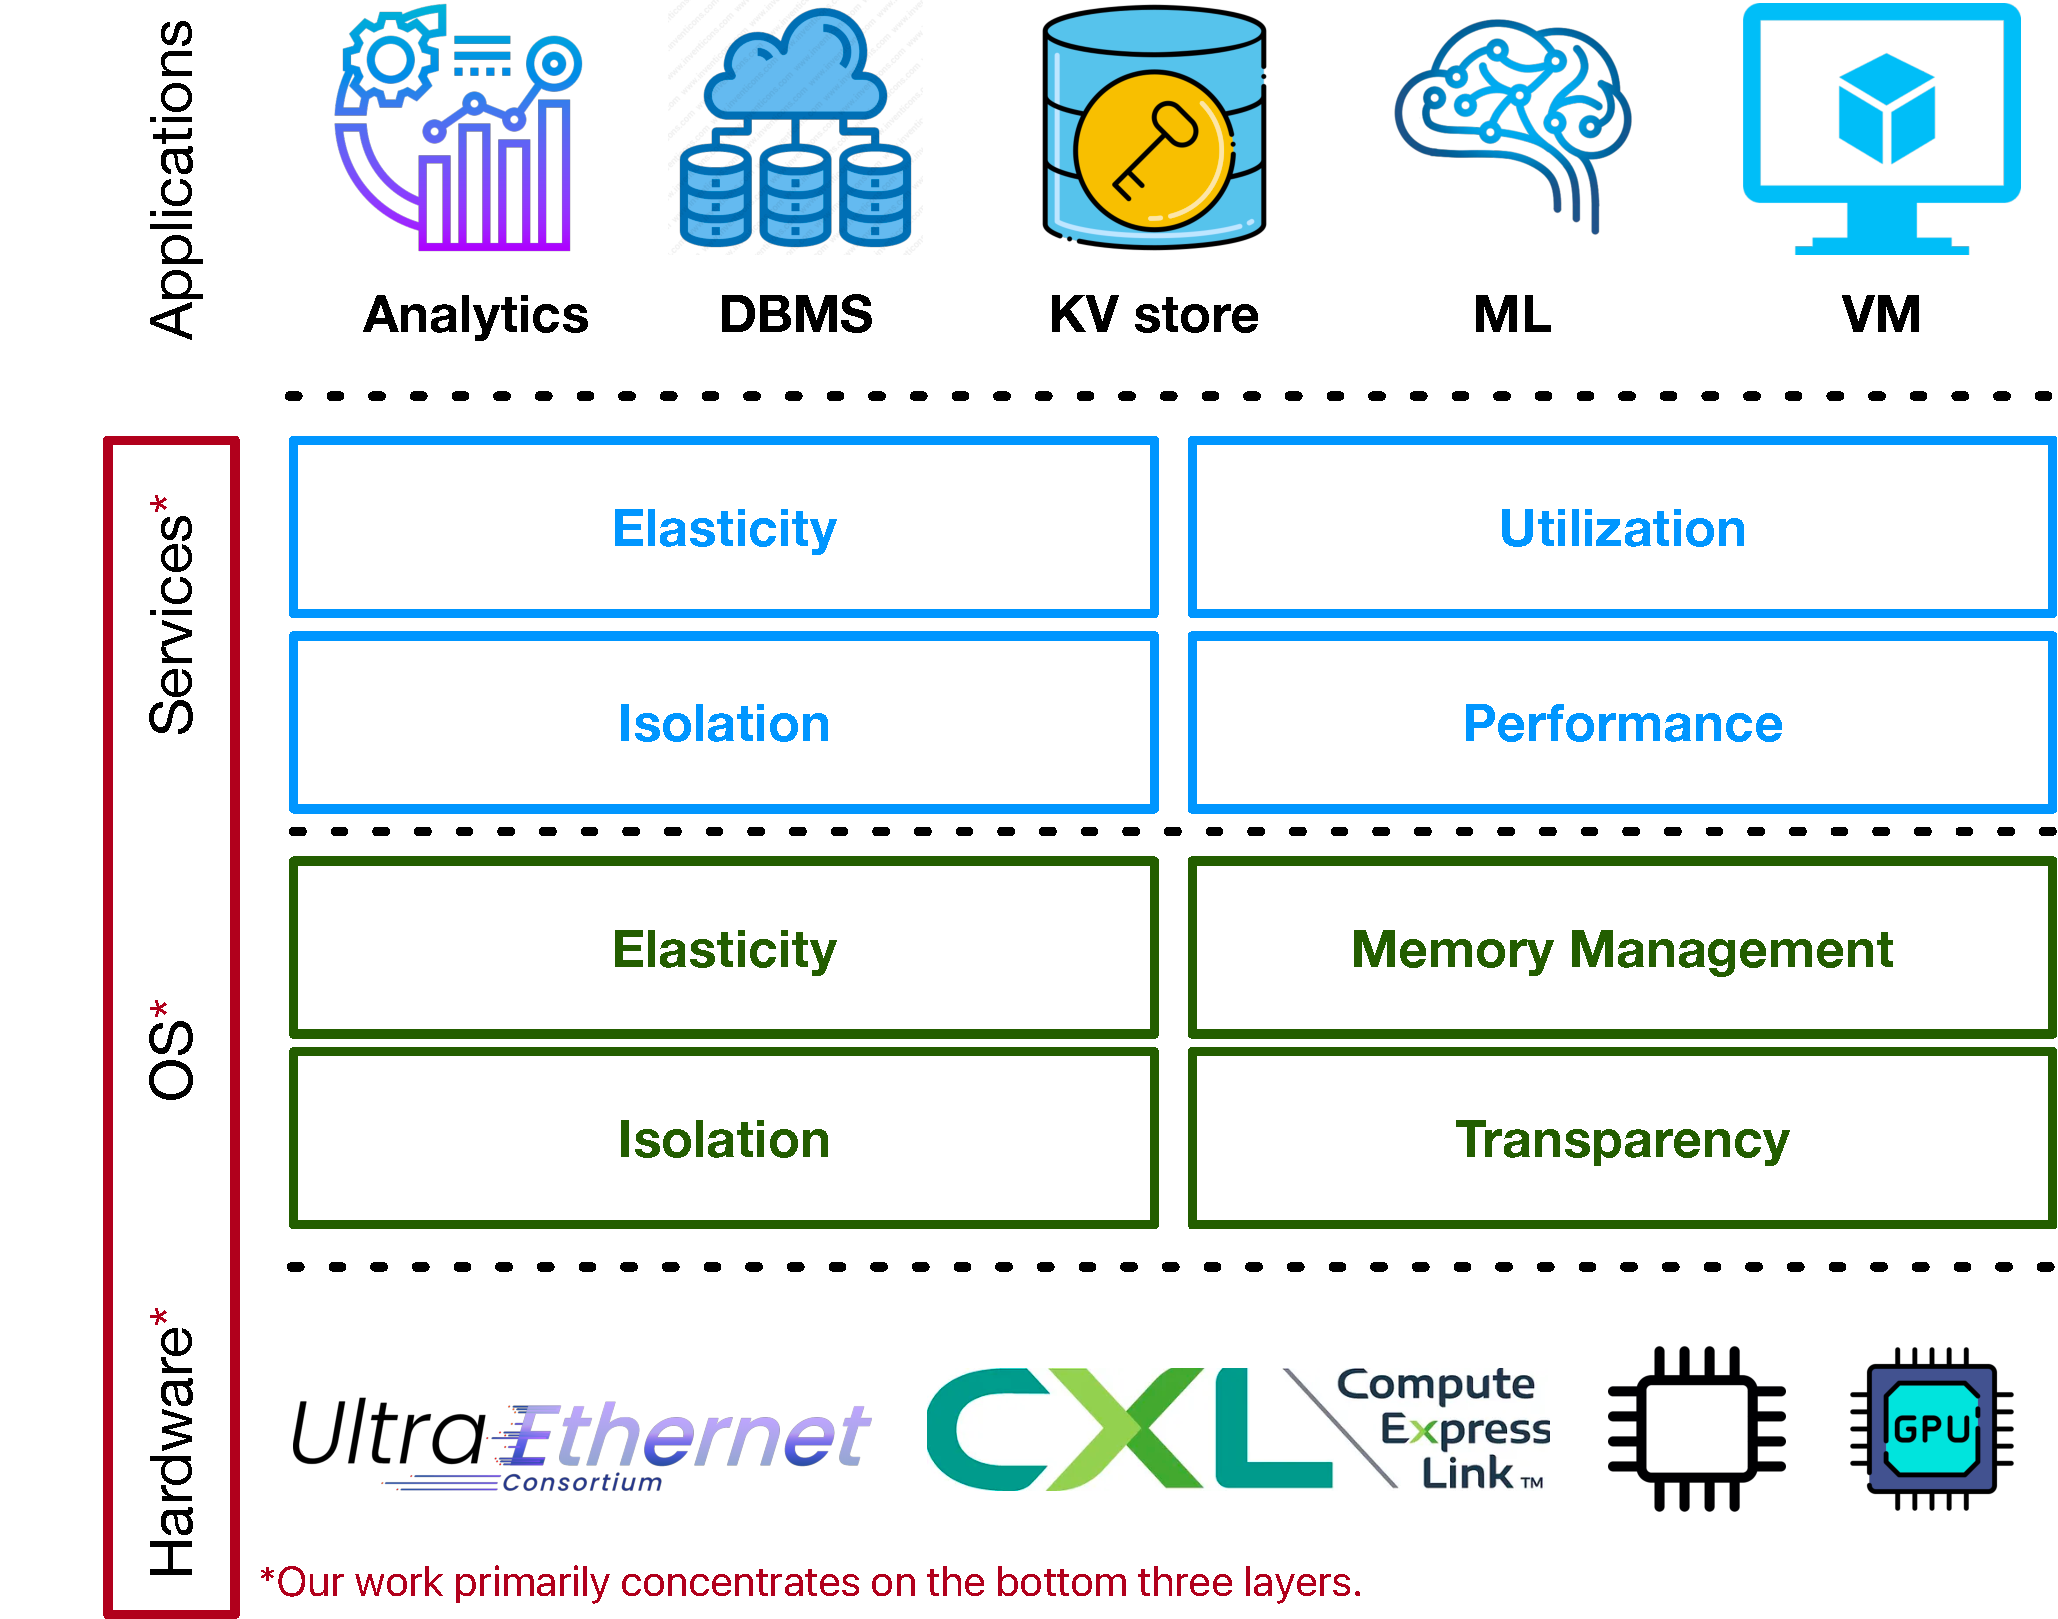
\includegraphics[width=0.8\columnwidth]{stack.pdf}
      \caption{\textbf{Cloud Stack of Disaggregated Architecture.}} \vspace{-1.0em}
      \label{fig:stack}
\end{figure}
The growing demand for scalable and efficient data center architectures has led to the emergence of resource disaggregation~\cite{mind, legoos, disagg, memdisagg1, memdisagg2, memdisagg3, memdisagg4, memdisagg5, memdisagg6}. This modern paradigm represents a significant shift from traditional monolithic server architectures. In conventional setups, servers are typically equipped with a fixed combination of compute, memory, and storage resources. In contrast, resource-disaggregated systems physically separate these resources and distribute them across various interconnects, such as networks~\cite{disagg, legoos, mind}, CXL~\cite{cxl, cxlasic}, and others. This separation allows for more flexible resource allocation and utilization.

Within the broader context of resource disaggregation in modern data center architectures, memory disaggregation~\cite{memdisagg1, memdisagg2, memdisagg3, memdisagg4, memdisagg5, memdisagg6} plays a crucial and foundational role. In traditional monolithic server configurations, memory often becomes a bottleneck, limiting the scalability and adaptability of applications. This issue has been frequently observed and reported in production data centers~\cite{memory1, memory2, memory3, memory4, memory5, memory6, memory7, memory8, memory9, memory10}. By decoupling memory resources from compute and storage elements and presenting them as pooled, disaggregated resources~\cite{pool1, pool2}, data centers can achieve increased efficiency, scalability, and adaptability. Memory-intensive applications~\cite{redis, ramcloud, sparkmemory} can access the memory they need on demand, without being constrained by the limitations of individual servers.

Memory disaggregation is the first step toward realizing the full potential of resource disaggregation, enabling data centers to efficiently allocate and utilize resources based on dynamic application needs. This ultimately leads to improved performance and better resource utilization.


\section{Limitations of Existing Approaches}

While resource disaggregation offers numerous advantages, transitioning existing applications to a disaggregated architecture is far from straightforward. Recent research has explored various approaches to address this challenge. Some efforts focus on adapting applications to optimize their use of disaggregated memory~\cite{farm, aifm, sherman, existing1}, while others aim to transparently port applications, shifting the responsibility of mitigating performance penalties—arising from the mismatch between disaggregated architectures and traditional software interfaces—to the service or operating system layer~\cite{mind, legoos, fastswap, infiniswap, runtime1, runtime2}.

The core issue lies in the fundamental mismatch between the existing cloud stack, designed for monolithic architectures, and the requirements of disaggregated architectures (Figure \ref{fig:stack}). The current cloud and hardware stacks are not inherently aware of the unique characteristics of disaggregated memory, leading to distinct challenges across different layers of the stack:

\paragraphb{Application interface} In disaggregated architectures, applications face unique challenges compared to traditional monolithic systems. The primary difference is resource distribution: compute, memory, and storage are spread across multiple nodes instead of centralized in one server. This requires complex communication and data management strategies to handle increased latency and resource management needs. In contrast, monolithic architectures offer integrated resources, simplifying application interaction. Adapting to disaggregated systems involves significantly redesigning applications for effective resource utilization and management.

\paragraphb{OS support} Unlike monolithic servers where the OS manages resources within a single server, the placement and function of the OS in disaggregated architectures are still subjects of debate in both industry and academia. Options include centralizing the OS at a single point~\cite{mind} in the architecture or disaggregating its functions across different resource nodes~\cite{legoos}.

\paragraphb{Performance overheads of disaggregation} Transitioning existing applications to a disaggregated architecture transparently introduces a spectrum of performance challenges. These include, but are not limited to, managing memory partitioning~\cite{jiffy} and addressing applications with irregular memory access patterns~\cite{chase}. Various other issues, such as latency sensitivity, bandwidth limitations, and the overhead of remote resource management, compound this complexity. These factors contribute to the overall performance penalty that disaggregated systems must carefully consider and mitigate.

\paragraphb{Future interconnects} Using networks as interconnects for resource disaggregation has been a subject of exploration in academia and industry. However, networks have inherent challenges, such as performance slowdowns compared to intra-server resource access and a lack of inherent coherency. Advanced hardware technologies like Compute Express Link (CXL)~\cite{cxl, cxlasic, pond} offer promising enhancements with faster access times and hardware-supported cache coherence. Yet, the current state of hardware prototypes and software support for these technologies remains limited.

\section{Thesis Overview}

In this dissertation, we attempt to take a top-down approach and explore the optimal memory management solutions for three most significant layers, i.e. Service, OS and Hardware layers of disaggregated memory architectures.

\subsection{Memory management as a Service}
With least modification to lower layers such as OS/Hardware, we explore the design requirement and challenges in provoding memory management as a service. We proposed an end-to-end system design called Jiffy, which enables multiple application/tasks multiplex memory in a elastic manner. Jiffy also provides multiple popular data structure interface and can be easily applied to existing cloud applications.
\subsection{In-network memory management OS-design}
As we decouple compute and memory resources in disaggregated architecture. There is no single host as if in monolithic architecture in order to implement the key unit of resource management - the operating system. We proposal a new generation operating system design by placing OS functionality inside the interconnects. We start by a system called MIND, addressing the basic problems in memory management, such as memory address translation, memory protection, and cache coherence between multiple hosts. Such resource decoupling and in-network memory management serves well for cache-friendly workload, but performs poor for cache-friendly workload due to the back-and-forth communication over the slower interconnects. We then develop optimizations for dealing with cache-unfriendly workloads. We design and implement a near memory accelerator from scratch, named PULSE. PULSE analyzes popular pointer traversal applications and identify a common but simple interface that can be easily integrated into existing cloud applications.
\subsection{Memory management adaptation for new-generation interconnects}
In prior work~\cite{mind,legoos}, ethernet is considered as the most popular interconnect for disaggregated data centers. However, as new memory interconnects are emerging, such as Compute Express Link(CXL), new adaptation of memory management needs to be made regarding the new interconnect interface. Within the context of disaggregated architecture, new problems arises such as how can the applications leverage multiple tiers of memory. Therefore, we start with a perfomance analysis on CXL 1.1 single host extended memory, and then we propose a new system design that integrates disaggregated CXL memory pool with today's emerging popular application - LLM inference.

\section{Outline and Previously Published Work}

This dissertation is organized as follows. Chapter~\ref{chap:service} introduces Jiffy, a distributed memory management system that decouples memory capacity and lifetime from compute in the serverless paradigm. Chapter~\ref{chap:os} describes two innovated system design: (1) MIND, a rack-scale memory disaggregation system that uses programmable switches to embed memory management logic in
the network fabric. (2) PULSE, a framework centered on enhancing in-network optimizations for
irregular memory accesses within disaggregated data centers. Chapter ~\ref{chap:hardware} presents our exploration in latest Compute Express Link(CXL) hardware. We conclude with our contributions and possible future work directions in Chapter~\ref{chap:future}.

Chapter~\ref{chap:service} revises material from ~\cite{jiffy}. Chapter~\ref{chap:os} revises material from ~\cite{mind} and ~\cite{chase}. Finally, Chapter~\ref{chap:hardware} revises material from ~\cite{cxleurosys}.

\chapter{Service Layer: Memory Management as a Service}
\label{chap:service}

\begin{figure}[t]
  \centering
  \subfigure[\scriptsize Intermediate data (normalized by mean usage)] {
    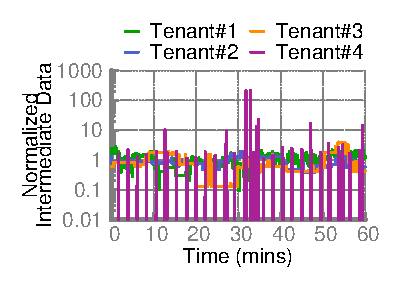
\includegraphics[width = 0.45\textwidth]{fig/jiffy/ephemeral_avg}
    \label{fig:ephemeral-avg}
  }
  \subfigure[\scriptsize Cumulative intermediate data (normalized by peak usage)] {
    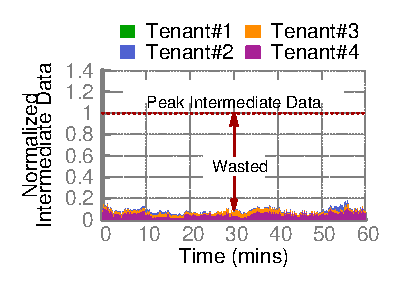
\includegraphics[width = 0.45\textwidth]{fig/jiffy/ephemeral}
    \label{fig:ephemeral-cum}
  }
  \caption[Snowflake workload anaylsis.]{\small{Analysis of production workloads from Snowflake~\cite{snowset} for four tenants over a $1$ hour window: (a) the ratio of peak to average storage usage for a job can vary by an order of magnitude during its execution; and (b) provisioning for peak usage results in average utilization $<10\%$. Across all tenants, the average utilization is $19\%$.}}\label{fig:ephemerals}%\vspace{-1.25em}
\end{figure}

Today's cloud applications rely heavily on the service layer~\cite{service1, service2, service3, service4, service5}, which sits above the OS layer and is divided into three sub-layers: Infrastructure as a Service (IaaS), Platform as a Service (PaaS), and Software as a Service (SaaS). Infrastructure as a Service (IaaS)~\cite{iaas1, iaas2} is a model where organizations outsource essential computing resources—such as storage, hardware, servers, and networking—to a service provider. The provider manages and maintains the infrastructure, while clients typically pay based on usage. This layer offers greater flexibility compared to the OS, enabling it to provide adaptable services that cater to the specific needs of various applications. However, this flexibility may require significant modifications to applications that do not utilize similar programming interfaces.

Migrating general cloud applications to disaggregated architectures presents challenges due to the substantial differences in the underlying infrastructure, such as physically decoupled resources and performance variability within interconnects. Rather than directly modifying applications to accommodate these new architectures, a more efficient approach is to provide \textbf{Memory Management as a Service} (MMaaS), which can be utilized by multiple applications. 

In this chapter, we begin by exploring the memory management service design for data analytics applications in serverless computing~\cite{starling, locus, pocket, flint, sparkonlambda, cirrus, excamera, pywren, numpywren, gg, athena, aurora, azuresqldw, cloudburst, snowset, caerus}. Recent advances in serverless analytics have shown the benefits of leveraging serverless architectures for resource- and cost-efficient data analytics. In these systems, remote, low-latency, high-throughput disaggregated memory is employed to store intermediate states for inter-task\footnote{Despite differences in their underlying programming models and semantics, existing distributed programming frameworks share a common structure (Figure~\ref{fig:example}). Specifically, a job is divided into multiple \textit{tasks}, which may be organized into several stages or structured as a directed acyclic graph (DAG). During execution, each task produces \textit{intermediate} data, which is partitioned upon task completion. This partitioned data is then exchanged with tasks in subsequent stages, enabling efficient data processing across the distributed system.} communication and multi-stage jobs, extending the lifetime of data beyond the task that produced it. This natural separation of compute and memory makes serverless computing an ideal candidate for harnessing disaggregated memory architectures.


Serverless analytics applications\cite{starling, shuffling, pocket, cirrus} handle user requests in the form of jobs, each defining its memory needs upon creation. The dilemma of balancing performance with resource efficiency for job-level memory allocation has been extensively studied ~\cite{elasticquery, qoop}. If a job is based on average demand, performance may decline during peak demand periods due to inadequate memory, causing data spillage to slower secondary storage, such as SSDs. Conversely, allocating memory for peak demands leads to underutilization of resources when the actual demand is below peak. Evaluations on Snowflake's workload, as shown in ~\cite{elasticquery}, indicate a significant fluctuation in the ratio of peak to average demands, sometimes varying by two orders of magnitude within minutes.

Designing a memory management service for such systems is a non-trivial task. We begin by outlining the essential requirements for memory management in disaggregated environments, focusing on the unique challenges posed by disaggregation:

\paragraphb{Elasticity}  Memory usage in modern computing is highly variable, with applications facing fluctuating demands~\cite{jiffy}. Elasticity enables dynamic memory allocation based on current needs, optimizing resource utilization. Applications like data analytics consist of jobs with multiple tasks that communicate via intermediate memory. Traditional solutions allocate memory at the job level, where jobs specify their requirements before execution, and the system reserves that amount for the job's duration~\cite{pocket}. This approach creates a tradeoff: allocating for average demand risks performance degradation due to swapping data to slower storage (e.g., S3), as shown in Figure~\ref{fig:ephemeral-avg}, while allocating for peak demand leads to resource waste (Figure~\ref{fig:ephemeral-cum}). Recent studies report that intermediate data sizes can vary by orders of magnitude during a job's lifetime~\cite{snowset}. For example, Figure~\ref{fig:ephemerals} shows that in a Snowflake dataset with over 2000 tenants, peak-to-average memory demand can vary by two orders of magnitude within minutes, resulting in performance degradation and resource inefficiency in job-level allocations.

\paragraphb{Isolation} The second requirement is the isolation between different compute tasks. Since multiple computing threads can be using the same disaggregated memory pool, it's essential to multiplex between applications to improve resource efficiency but at the same time keep the memory of different threads isolated from each other, which means that the memory usage of a particular application should not affect other existing applications. The number of tasks reading and writing to the shared disaggregated memory can change rapidly in serverless analytics which makes the problem even more severe.

\paragraphb{Lifetime management}
Decoupling compute tasks from their intermediate storage means that the tasks can fail independent of the intermediate data, therefore we need mechanisms for explicity lifetime management of intermediate data.

\paragraphb{Data repartitioning}
Decoupling tasks from their intermediate data also means that data partitioning upon elastic scaling of memory capacity becomes challenging, especially for certain data types used in serverless analytics (e.g. key-value store). If it's the application's responsibility to perform such repartitioning, it will involve large network transfers betweem compute tasks and the far memory system and massive read/write operations every time the capacity is scaled. What's more, the application need to implement different partitioning strategies for different kind of data structures used. Therefore, new mechansims to efficiently enable data partitioning within the far memory system is essential.


We present Jiffy, an elastic disaggregated-memory system for stateful serverless analytics. Jiffy allocates memory resources at the granularity of small fixed-size memory blocks - multiple memory blocks store intermediate data for individual tasks within a job. Jiffy design is motivated by virtual memory design in operating systems that also does memory allocation to individual process at the granularity of fixed-size memory blocks(pages). Jiffy adapts this design to stateful serverless analytics. Performing resource allocation at the granularity of small memory blocks allows Jiffy to elastically scale memory resources allocated to individual jobs without a priori knowledge of intermediate data sizes and to meet the instantaneous job demands at seconds timescales. As a result, Jiffy can efficiently multiplex the available faster memory capacity across concurrently running jobs, thus minimizing the overheads of reads and writes to significantly slower secondary storage (e.g., S3 or disaggregated storage)


\begin{figure}
  \centering
  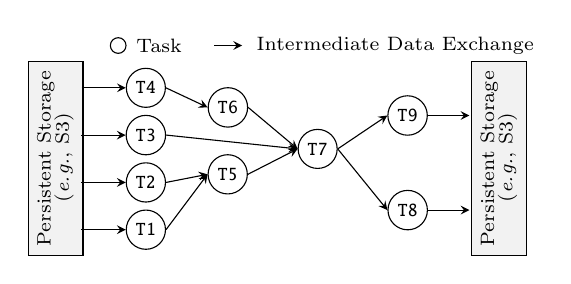
\begin{tikzpicture}[font=\scriptsize, yscale=0.8, task/.style={draw, circle, align=center, inner sep=2pt}]
    \node[task] (t1) {\texttt{T1}};
    \node[task, above=0.25em of t1] (t2) {\texttt{T2}};
    \node[task, above=0.25em of t2] (t3) {\texttt{T3}};
    \node[task, above=0.25em of t3] (t4) {\texttt{T4}};
    \node[task, right=1.5em of t1, yshift=2em] (t5) {\texttt{T5}};
    \node[task, right=1.5em of t3, yshift=1em] (t6) {\texttt{T6}};
    \node[task, right=4.75em of t3, yshift=-0.5em] (t8) {\texttt{T7}};
    \node[task, right=8em of t2, yshift=-1em] (t10) {\texttt{T8}};
    \node[task, right=8em of t4, yshift=-1em] (t12) {\texttt{T9}};
    
    
    \draw[-stealth] (t1.east) -- (t5.west);
    \draw[-stealth] (t2.east) -- (t5.west);
    \draw[-stealth] (t3.east) -- (t8.west);
    \draw[-stealth] (t4.east) -- (t6.west);
    \draw[-stealth] (t5.east) -- (t8.west);
    \draw[-stealth] (t6.east) -- (t8.west);
    \draw[-stealth] (t8.east) -- (t10.west);
    \draw[-stealth] (t8.east) -- (t12.west);
    
    \node[draw, fill=gray!10, left=2.25em of $(t3)!0.5!(t2)$] {\rotatebox{90}{Persistent Storage}\rotatebox{90}{\quad\quad(\eg, S3)}};
    \node[draw, fill=gray!10, right=11.75em of $(t3)!0.5!(t2)$] {\rotatebox{90}{Persistent Storage}\rotatebox{90}{\quad\quad(\eg, S3)}};
    
    \draw[-stealth] ($(t1.west)+(-1.6em, 0)$) -- (t1.west);
    \draw[-stealth] ($(t2.west)+(-1.6em, 0)$) -- (t2.west);
    \draw[-stealth] ($(t3.west)+(-1.6em, 0)$) -- (t3.west);
    \draw[-stealth] ($(t4.west)+(-1.6em, 0)$) -- (t4.west);
    \draw[-stealth] (t10.east) -- ($(t10.east)+(1.5em, 0)$);
    \draw[-stealth] (t12.east) -- ($(t12.east)+(1.5em, 0)$);
    
    \node[task, above=0.5em of t4, xshift=-1em] (tl) {};
    \node[right=0em of tl] (t) {Task};
    \node[right=2em of t] {Intermediate Data Exchange};
    \draw[-stealth] ($(t)+(2em, 0em)$) -- ($(t)+(3em, 0em)$);
    
  \end{tikzpicture}
  \caption[Execution DAG example for a typical analytics job.]{\small\textbf{Execution DAG example for a typical analytics job.} Intermediate data exchange across tasks occurs via \jiffy.}
  \label{fig:example}
  \label{fig:query-example}
\end{figure}

\section{\jiffy Design}
\label{sec:jiffydesign}

This section explains how \jiffy uses hierarchical addressing, intermediate data lifetime management, and flexible data repartitioning to meet these requirements. We illustrate this with Figure~\ref{fig:query-example}, which depicts the execution plan of a typical analytics job. The plan is represented as a directed acyclic graph (DAG), where nodes are computation tasks (implemented as serverless functions\footnote{Functions refer to basic computation units in serverless architectures, such as Amazon Lambdas~\cite{alambda}, Google Functions~\cite{googlefunctions}, and Azure Functions~\cite{azureFunctions}}), and edges represent intermediate data exchanged via \jiffy.


\begin{figure}[t]
  \centering
  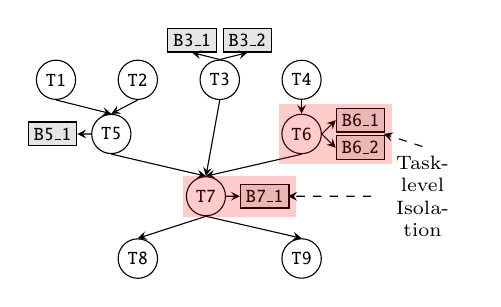
\begin{tikzpicture}[font=\scriptsize, yscale=0.75, task/.style={draw, circle, align=center, inner sep=2pt}, block/.style={draw, align=center, fill=gray!20, inner sep=2pt}]
    \node[task] (t1) {\texttt{T1}};
    \node[task, right=1.5em of t1] (t2) {\texttt{T2}};
    \node[task, right=1.5em of t2] (t3) {\texttt{T3}};
    \node[task, right=1.5em of t3] (t4) {\texttt{T4}};
    \node[task, below=0.5em of t1, xshift=2em] (t5) {\texttt{T5}};
    \node[task, below=0.5em of t4] (t6) {\texttt{T6}};
    \node[task, below=2.75em of t3, xshift=-0.5em] (t8) {\texttt{T7}};
    \node[task, below=5em of t2] (t10) {\texttt{T8}};
    \node[task, below=5em of t4] (t12) {\texttt{T9}};
    
    \node[block, above=0.25em of t3, xshift=-1em] (t3b1) {\texttt{B3\_1}};
    \node[block, above=0.25em of t3, xshift=1em] (t3b2) {\texttt{B3\_2}};
    \node[block, left=0.5em of t5] (t5b1) {\texttt{B5\_1}};
    \node[block, right=0.5em of t6, yshift=0.5em] (t6b1) {\texttt{B6\_1}};
    \node[block, right=0.5em of t6, yshift=-0.5em] (t6b2) {\texttt{B6\_2}};
    \node[block, right=0.5em of t8] (t8b1) {\texttt{B7\_1}};

    \draw[-stealth] (t1.south) -- (t5.north);
    \draw[-stealth] (t2.south) -- (t5.north);
    \draw[-stealth] (t3.south) -- (t8.north);
    \draw[-stealth] (t4.south) -- (t6.north);
    \draw[-stealth] (t5.south) -- (t8.north);
    \draw[-stealth] (t6.south) -- (t8.north);
    \draw[-stealth] (t8.south) -- (t10.north);
    \draw[-stealth] (t8.south) -- (t12.north);
    
    \draw[-stealth] (t3.north) -- (t3b1.south);
    \draw[-stealth] (t3.north) -- (t3b2.south);
    \draw[-stealth] (t5.west) -- (t5b1.east);
    \draw[-stealth] (t6.east) -- (t6b1.west);
    \draw[-stealth] (t6.east) -- (t6b2.west);
    \draw[-stealth] (t8.east) -- (t8b1.west);
    
    \draw[thick, dashed, opacity=0] ($(t5.south west)+(-0.3em, -0.3em)$) rectangle node[midway, right] (t5a) {} ($(t5.north east)+(2.05em, 0.3em)$);
    \draw[thick, dashed, opacity=0, fill=red, fill opacity=0.2] ($(t6.south west)+(-0.3em, -0.75em)$) rectangle node[midway, right] (t6a) {} ($(t6.north east)+(2.75em, 0.75em)$);
    \draw[thick, dashed, opacity=0, fill=red, fill opacity=0.2] ($(t8.south west)+(-0.3em, -0.3em)$) rectangle node[midway, right] (t8a) {} ($(t8.north east)+(2.75em, 0.3em)$);
    
    \node[right=4em of t8a, text width=3em, align=center] (ri) {Task-level Isolation};
    \draw[-stealth, dashed] (ri.west) -- ($(t8a.east)+(1em,0em)$);
    \draw[-stealth, dashed] (ri.north) -- ($(t6a.east)+(1em,0em)$);
    
  \end{tikzpicture}
  \caption[Hierarchical addressing]{\textbf{Hierarchical addressing} for the job in Figure~\ref{fig:query-example}. \jiffy provides task-level resource isolation for ephemeral storage under each task address-prefix (\S\ref{ssec:hva}). Note that block addresses are only assigned to address-prefixes with currently allocated blocks; for tasks \texttt{T1}, \texttt{T2} and \texttt{T4}, blocks are directly read from persistent storage and not stored in \jiffy.}
  \label{fig:hina}
\end{figure}

\subsection{Hierarchical Addressing}
\label{ssec:hva}
Analytics jobs are often structured as multiple stages or a directed acyclic graph (DAG). In serverless analytics, where compute elasticity is key, each job can run tens to thousands of tasks~\cite{starling, locus, pocket, flint, sparkonlambda, cirrus, excamera, pywren, numpywren, gg, athena, aurora, azuresqldw, cloudburst, snowset}. Fine-grained resource allocation requires efficient mapping between tasks and their storage blocks, especially with rapidly changing task concurrency. High concurrency demands task-level isolation, ensuring that task arrival or departure doesn't affect others, avoiding performance degradation.

\jiffy adopts a hierarchical addressing mechanism, inspired by the Internet's IP addressing, to maintain task-to-storage mappings and ensure task-level isolation. \jiffy organizes intermediate data in a virtual address hierarchy based on task dependencies in the DAG. Internal nodes represent tasks, and leaf nodes represent \jiffy blocks storing data. Block addresses are defined by the hierarchy path, with task-generated prefixes. Dependencies between tasks are captured by edges between nodes. \jiffy builds this hierarchy from execution plans (e.g., AWS Step Functions, Azure Durable Functions) or dynamically deduces it via the \jiffy API, supporting dynamic query plans without predefined DAGs.

\paragraphb{Example} Figure~\ref{fig:hina} illustrates the \lh for the job in Figure~\ref{fig:example}. Internal nodes \texttt{T1}-\texttt{T9} represent tasks in the DAG, while leaf nodes \texttt{B3\_1}, \texttt{B3\_2}, etc., represent data blocks allocated by \jiffy for intermediate data storage. Edges like (\texttt{T1}, \texttt{T5}) and (\texttt{T2}, \texttt{T5}) indicate that \texttt{T5} depends on the intermediate data from both \texttt{T1} and \texttt{T2}. The full address of block \texttt{B6\_2} under \texttt{T6} is \texttt{T4.T6.B6\_2}, with \texttt{T4.T6} identifying all blocks under \texttt{T6}. \jiffy constructs the \lh either using the execution plan from Figure~\ref{fig:query-example} or deduces it dynamically. For instance, \sl can infer that since \texttt{T7}'s sub-tasks access data from \texttt{T3}, \texttt{T5}, and \texttt{T6}, these tasks must be its parents in the hierarchy.


By organizing intermediate data in a hierarchy, \jiffy manages resource allocation per address prefix. If one prefix spills to persistent storage (via Pocket), it doesn’t affect others. Blocks remain assigned until reclaimed or leases expire (\S\ref{ssec:mlm}), ensuring task-level isolation regardless of churn. Like virtual memory isolating processes, \jiffy uses hierarchical addressing to isolate tasks based on the job's structure.

Two design considerations arise: (1) \jiffy's fine-grained allocation is independent of fairness policies, which can be layered on top, and (2) address translation from virtual to physical storage happens at a centralized metadata server (like Pocket~\cite{pocket}), scaling to arbitrary DAG sizes. Despite added complexity, \jiffy scales to ${\sim}45$K requests/sec/core, sufficient for most deployments.

\paragraphb{Block sizing} Jiffy balances metadata storage and memory use with block sizes, like $128$MB in HDFS~\cite{hdfs}. Larger blocks reduce metadata but risk fragmentation, while smaller blocks improve utilization at a metadata cost. Jiffy mitigates this via fine-grained access and data repartitioning.

\paragraphb{Isolation granularity} Task-level isolation, where nodes in the hierarchy map to tasks, is default, but finer or coarser isolation (e.g., table-level or stage-level) can be configured via the \jiffy API.


\subsection{Data Lifetime Management}
\label{ssec:mlm}

\begin{figure}[t]
  \centering
  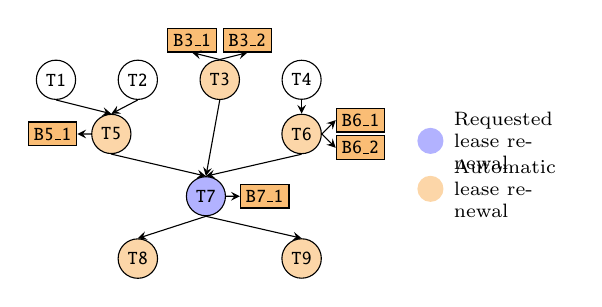
\begin{tikzpicture}[font=\scriptsize, yscale=0.75, task/.style={draw, circle, align=center, inner sep=2pt}, block/.style={draw, align=center, fill=gray!20, inner sep=2pt}]
    \node[task] (t1) {\texttt{T1}};
    \node[task, right=1.5em of t1] (t2) {\texttt{T2}};
    \node[task, fill=BurntOrange!30, right=1.5em of t2] (t3) {\texttt{T3}};
    \node[task, right=1.5em of t3] (t4) {\texttt{T4}};
    \node[task, fill=BurntOrange!30, below=0.5em of t1, xshift=2em] (t5) {\texttt{T5}};
    \node[task, fill=BurntOrange!30, below=0.5em of t4] (t6) {\texttt{T6}};
    \node[task, fill=blue!30, below=2.75em of t3, xshift=-0.5em] (t8) {\texttt{T7}};
    \node[task, fill=BurntOrange!30, below=5em of t2] (t10) {\texttt{T8}};
    \node[task, fill=BurntOrange!30, below=5em of t4] (t12) {\texttt{T9}};
    
    \node[block, fill=BurntOrange!50, above=0.25em of t3, xshift=-1em] (t3b1) {\texttt{B3\_1}};
    \node[block, fill=BurntOrange!50, above=0.25em of t3, xshift=1em] (t3b2) {\texttt{B3\_2}};
    \node[block, fill=BurntOrange!50, left=0.5em of t5] (t5b1) {\texttt{B5\_1}};
    \node[block, fill=BurntOrange!50, right=0.5em of t6, yshift=0.5em] (t6b1) {\texttt{B6\_1}};
    \node[block, fill=BurntOrange!50, right=0.5em of t6, yshift=-0.5em] (t6b2) {\texttt{B6\_2}};
    \node[block, fill=BurntOrange!50, right=0.5em of t8] (t8b1) {\texttt{B7\_1}};

    \draw[-stealth] (t1.south) -- (t5.north);
    \draw[-stealth] (t2.south) -- (t5.north);
    \draw[-stealth] (t3.south) -- (t8.north);
    \draw[-stealth] (t4.south) -- (t6.north);
    \draw[-stealth] (t5.south) -- (t8.north);
    \draw[-stealth] (t6.south) -- (t8.north);
    \draw[-stealth] (t8.south) -- (t10.north);
    \draw[-stealth] (t8.south) -- (t12.north);
    
    \draw[-stealth] (t3.north) -- (t3b1.south);
    \draw[-stealth] (t3.north) -- (t3b2.south);
    \draw[-stealth] (t5.west) -- (t5b1.east);
    \draw[-stealth] (t6.east) -- (t6b1.west);
    \draw[-stealth] (t6.east) -- (t6b2.west);
    \draw[-stealth] (t8.east) -- (t8b1.west);
    
    \draw[thick, dashed, opacity=0] ($(t8.south west)+(-0.3em, -0.3em)$) rectangle node[midway, right] (t8a) {} ($(t8.north east)+(2.05em, 0.3em)$);
%    
    \node[circle, fill=blue!30, right=6em of t8a, yshift=2em] (lr) {};
    \node[right=0em of lr, text width=4em] {Requested lease renewal};
    \node[circle, fill=BurntOrange!30, below=0.75em of lr] (ar) {};
    \node[right=0em of ar, text width=4em] {Automatic lease renewal};
    
  \end{tikzpicture}
  \caption[Lease Renewal via Address Hierarchy]{\textbf{Lease Renewal via Address Hierarchy.} Hierarchical addressing simplifies lease renewal in \jiffy (\S\ref{ssec:mlm}), since lease renewal for an address-prefix automatically implies renewals for all parent and descendent address-prefixes in the hierarchy.}\label{fig:mlm}
\end{figure}

Existing ephemeral storage systems manage data at the job level, reclaiming storage when the job deregisters. In serverless analytics, decoupled task execution and storage can lead to orphaned data. \jiffy addresses this by integrating lease management~\cite{gray1989leases, chubby, dhcplease} with hierarchical addressing for task-level data management. Each address prefix has a lease, and data is retained as long as the lease is renewed. Serverless platforms can trigger lease renewals during task monitoring.

Using the DAG hierarchy, \jiffy renews leases for dependent and ancestor tasks automatically, reducing overhead while preventing orphaned data. This strikes a balance between age-based eviction and explicit resource management, ensuring efficient reassignment of resources upon task or job failure.

\paragraphb{Example} In Figure~\ref{fig:query-example}, task \texttt{T7}'s job periodically renews the lease for the prefix \texttt{T4.T6.T7}\footnote{Task \texttt{T7} has four address prefixes; the job can renew any.}. Renewing \texttt{T7}'s lease also renews those for parent tasks (\texttt{T3}, \texttt{T5}, \texttt{T6}) and descendants (\texttt{T8}, \texttt{T9}), as shown in Figure~\ref{fig:mlm}. This ensures that both parent and descendant tasks' data remain accessible.

\paragraphb{Lease duration} Lease duration trades off control plane bandwidth with system utilization. Longer leases reduce network traffic but may delay resource reclamation. Configuring lease durations, as studied in prior work~\cite{chubby, gray1989leases}, allows \jiffy to meet specific deployment goals.






\subsection{Flexible Data Repartitioning}
\label{ssec:fdr}

Decoupling compute tasks from their intermediate data in serverless analytics introduces challenges in achieving fine-grained elasticity for ephemeral storage. Specifically, when storage is allocated or deallocated for a task, the intermediate data must be efficiently repartitioned across available blocks. However, due to the decoupling of compute from storage and the large number of concurrent tasks, this repartitioning should not be managed by the application itself. For instance, many serverless analytics systems~\cite{locus, pocket} rely on key-value stores for intermediate data. If compute tasks were responsible for repartitioning during memory scaling, they would need to read key-value pairs over the network, compute new partitions based on updated memory, and write the data back to the store—resulting in significant network latency and bandwidth overhead.

\jiffy supports various data structures commonly used in data analytics frameworks, including files~\cite{sparkonlambda, athena, aurora, azuresqldw, snowset}, key-value pairs~\cite{pywren, locus, starling, gg, cirrus, cloudburst, pocket}, and queues~\cite{flint, excamera}. Analytics jobs using these structures can delegate intermediate data repartitioning to \jiffy during resource allocation or deallocation. Each block in a \jiffy data structure tracks its own memory usage. When usage exceeds a predefined threshold, \jiffy allocates a new block to the corresponding address-prefix\footnote{Similar to existing systems~\cite{elasticache, redis, ramcloud, pocket}, \sl can scale cluster capacity by adding or removing servers based on free blocks. Here, we focus on fine-grained elasticity.}. The overloaded block triggers a data-specific repartitioning process, moving some of its data to the newly allocated block. Conversely, when block usage drops below a low threshold, \jiffy merges it with another low-usage block before deallocating the unused block. By allowing the block itself, rather than the compute task, to handle repartitioning, \jiffy minimizes network and compute overhead for the task. Repartitioning is done asynchronously, allowing data access to continue with minimal impact on performance.

Jiffy’s supported data structures enable the serverless execution of powerful distributed frameworks like MapReduce~\cite{mapreduce,spark}, Dryad~\cite{dryad}, StreamScope~\cite{streamscope}, and Piccolo~\cite{piccolo}. Since files, queues, and key-value stores in analytics frameworks require relatively simple repartitioning (unlike complex structures such as B-trees), serverless applications can leverage \jiffy’s flexible repartitioning mechanism without requiring any modifications.


\paragraphb{Thresholds for Elastic Scaling} In \jiffy, the high and low thresholds play a crucial role in balancing network bandwidth usage, task performance, and overall system utilization. Setting thresholds too high or too low can impact elastic scaling behavior—if scaling is triggered too infrequently, it may reduce network traffic, but it can also result in inefficient block utilization, such as numerous underutilized blocks. The optimal values for these thresholds depend heavily on the specific workload characteristics, as highlighted in previous studies~\cite{mongo-shard, ceph-shard}. To accommodate diverse workloads, \jiffy makes these thresholds fully configurable, allowing users to adjust them to suit their performance and efficiency needs.


\section{\jiffy Implementation}
\label{sec:jiffyimplementation}

\jiffy builds on Pocket~\cite{pocket}, inheriting its scalable and fault-tolerant metadata plane, multi-tiered data storage, system-wide capacity scaling, and analytics execution model. However, \jiffy introduces hierarchical addressing, lease management, and efficient data repartitioning to address the unique challenges of serverless environments. Below, we describe the \jiffy interface and implementation, highlighting these key features.

\subsection{\jiffy Interface}
\label{ssec:jiffyapi}

\begin{table}[t]
    \centering
    \footnotesize
    \begin{tabular}{c|l}
        \hline
        \textbf{API Group} & \textbf{Function Signature} \\
        \hline
        \multicolumn{1}{c|}{} & connect(honeycombAddress) \\
        \hline
        \multirow{4}{*}{Address Hierarchy} 
            & createAddrPrefix(addr, parent, optionalArgs) \\
            & createHierarchy(dag, optionalArgs) \\
            & flushAddrPrefix(addr, externalPath) \\
            & loadAddrPrefix(addr, externalPath) \\
        \hline
        \multirow{2}{*}{Lease Operations} 
            & leaseDuration = getLeaseDuration(addr) \\
            & renewLease(addr) \\
        \hline
        \multirow{3}{*}{Data Structure}
            & ds = initDataStructure(addr, type) \\
            & listener = ds.subscribe(op) \\
            & notif = listener.get(timeout) \\
        \hline
    \end{tabular}
    \caption[\jiffy User-facing API]{\textbf{\jiffy User-facing API}: Functions for connecting, managing address hierarchies, handling leases, and interacting with data structures.}
    \label{table:api}
\end{table}



We describe the \jiffy interface in terms of its user-facing API (Table~\ref{table:api}) and internal API (Figure~\ref{fig:blockapi}).

\paragraphb{User-facing API} The user-facing interface (Table~\ref{table:api}) is centered around two core abstractions: \textit{hierarchical addresses} and \textit{data structures}. Jobs can create a new address-prefix using \texttt{createAddrPrefix}, specifying the parent prefix along with optional parameters such as initial capacity. The \texttt{createHierarchy} function generates a complete hierarchy from an execution plan (DAG), while \texttt{flush} and \texttt{load} facilitate persisting and retrieving address-prefix data from external storage (e.g., S3). Three built-in data structures can be initialized for an address-prefix via \texttt{initDataStructure}, and new structures can be defined using the internal API.

Similar to existing systems~\cite{redis, sns}, \jiffy’s data structures provide a notification interface, allowing tasks that consume intermediate data to be informed when new data is available. For example, a task can \texttt{subscribe} to write operations on its parent task’s data structure and receive a \texttt{listener} handle. When data is written, \jiffy asynchronously notifies the \texttt{listener}, which the task can access via \texttt{listener.get()}.


\begin{figure}[h]
  \centering
  \begin{tabular}{c}
  {\begin{lstlisting}[frame=single, gobble=4, linewidth=20em]
    block = ds.getBlock(op, args) // Get block
    block.writeOp(args) // Perform write
    data = block.readOp(args) // Perform read
    block.deleteOp(args) // Perform delete
  \end{lstlisting}}
  \end{tabular}
  \caption[\jiffy Internal API]{\textbf{\jiffy Internal API.} The block interface is used internally in \jiffy to implement the data structure APIs.}  
  \label{fig:blockapi}
\end{figure}

\paragraphb{Internal API} The data layout within \jiffy blocks is tailored to the specific data structure that owns it. Therefore, \jiffy blocks expose a set of data structure-specific \textit{operators} (Figure~\ref{fig:blockapi}) that define how requests are \textit{routed} across blocks and how data is \textit{accessed} or \textit{modified}. These operators are used internally by \jiffy for its built-in data structures (\S\ref{ssec:jiffymodels}) and are not directly exposed to jobs.

The \texttt{getBlock} operator determines the target block for an operation based on the operation type and its arguments (e.g., key hashes for a KV-store), returning a handle to the appropriate block. Each \jiffy block provides \texttt{writeOp}, \texttt{readOp}, and \texttt{deleteOp} operators, which implement data structure-specific access logic (e.g., \texttt{get}, \texttt{put}, and \texttt{delete} in a KV-store). Jiffy executes these operators \textit{atomically} using sequence numbers but does not support atomic transactions across multiple operators.



\begin{table*}[t]
  \centering
  \small
  \caption[\jiffy Data Structure Implementations]{\textbf{\jiffy Data Structure Implementations}. See \S\ref{ssec:jiffymodels} for details.}
  \label{table:ds}
  \begin{tabular}{c|l|c|c|c|l|c}
    \hline
    \multicolumn{2}{c|}{\textbf{Data Structure}} & \textbf{writeOp} & \textbf{readOp} & \textbf{deleteOp} & \textbf{getBlock} & \textbf{repartition} \\
    \hline
    \hline
    \multirow{3}{*}{\rotatebox[origin=c]{90}{\footnotesize Built-in}} 
      & File (\S\ref{sssec:bsp}) & \texttt{write} & \texttt{read} & \texttt{-} & File offsets. & \xmark \\\cline{2-7}
      & FIFO Queue (\S\ref{sssec:dflow}) & \texttt{enqueue} & \multicolumn{2}{c|}{\texttt{dequeue}} & Tail/head. & \xmark \\\cline{2-7}
      & KV-Store (\S\ref{sssec:piccolo}) & \texttt{put} & \texttt{get} & \texttt{delete} & Key hash. & \checkmark \\
    \hline
    \multicolumn{7}{c}{\textit{Custom data structures}} \\
    \hline
  \end{tabular}
\end{table*}


\begin{figure}[h]
  \centering
  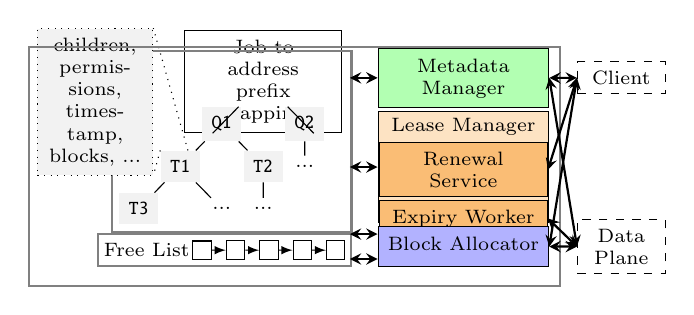
\begin{tikzpicture}[font=\scriptsize, yscale=0.9, level distance=1.7em, level 1/.style={sibling distance=3em}, level 2/.style={sibling distance=3em}, level 3/.style={sibling distance=3em}]
  	\node (root) [draw, text width=5em, align=center] {Job to address\\prefix mapping}
  	   child { node[fill=gray!10] (app1) {\aa}
        child { node[fill=gray!10] (g1) {\texttt{T1}} 
          child { node[fill=gray!10] (task1) {\texttt{T3}} }
          child { node {...} }
        }
        child { node[fill=gray!10] (g2) {\texttt{T2}} 
          child { node (r) {...} }
        }
      }
      child {
        node[fill=gray!10] (app2) {\ab}
        child { node {...} }
      };
    \draw[black, thick, color=gray] ($(app1.north west)+(-3.25em,2.25em)$) rectangle node[midway, right] (tree-border) {} ($(r.south east)+(2.5em,-0.5em)$);
  	\node[draw, dotted, fill=gray!10, text width=3.5em, align=center, left=0.25em of g1.north west, yshift=1.75em] (internal) {children, permissions, timestamp, blocks, ...};
  	\draw[dotted] ($(g1.north west)+(1em, 0em)$) -- (internal.north east);
  	\draw[dotted] (g1.north west) -- (internal.south east);
  	

    \node[draw, below=0.75em of r.south east, xshift=-2.9em] (head) {};
    \node[draw, right=0.5em of head] (mid1) {};
    \node[draw, right=0.5em of mid1] (mid2) {};
    \node[draw, right=0.5em of mid2] (mid3) {};
    \node[draw, right=0.5em of mid3] (tail) {};

    \draw[-latex] (head.east) -- (mid1.west);
    \draw[-latex] (mid1.east) -- (mid2.west);
    \draw[-latex] (mid2.east) -- (mid3.west);
    \draw[-latex] (mid3.east) -- (tail.west);

    \node[left=-0.25em of head] (flist) {Free List};

    \draw[black, thick, color=gray] ($(flist.north west)+(0.15em, 0em)$) rectangle ($(tail.south east)+(0.2em, -0.25em)$);
  	
  	\node[draw, fill=green!30, text width=5.5em, align=center] (fs-api) at ([xshift=8em, yshift=2.55em]tree-border){$\strut$Metadata Manager};
  	
  	\node[draw, fill=BurntOrange!20, minimum height=4em, text width=5.5em, align=center, below=0.1em of fs-api] (lm) {};
  	\node[text width=5.5em, align=center, below=-0.1em of lm.north] (lm-title) {Lease Manager};
  	\node[draw, fill=BurntOrange!50, text width=5.4em, align=center, below=-0.1em of lm-title] (lm-renewal) {Renewal Service};
  	\node[draw, fill=BurntOrange!50, text width=5.4em, align=center, below=0.1em of lm-renewal] (lm-expiry) {Expiry Worker};
  	
  	\node[draw, fill=blue!30, minimum height=1em, text width=5.5em, align=center, below=0.1em of lm] (sm) {$\strut$Block Allocator};
  	
  	\draw[black, thick, color=gray] ($(app1.north west)+(-6.25em,2.4em)$) rectangle node[midway, right] (dir-border) {} ($(sm.south east)+(0.4em,-0.75em)$);
  	
  	\node[draw, dashed, text width=2.5em, align=center, right=1em of fs-api] (client) {Client};
  	\node[draw, dashed, text width=2.5em, align=center, right=1em of sm] (ss) {Data Plane};
  	
  	\draw[stealth-stealth, thick] (fs-api.east) -- (client.west);
  	\draw[stealth-stealth, thick] (lm-renewal.east) -- (client.west);
  	\draw[stealth-stealth, thick] (sm.east) -- (client.west);
  	\draw[stealth-stealth, thick] (fs-api.east) -- (ss.west);
  	\draw[stealth-stealth, thick] (lm-expiry.east) -- (ss.west);
  	\draw[stealth-stealth, thick] (sm.east) -- (ss.west);
  	
  	\draw[stealth-stealth, thick] (fs-api.west) -- ($(fs-api.west)+(-1em, 0em)$);
  	\draw[stealth-stealth, thick] (lm.west) -- ($(lm.west)+(-1em, 0em)$);
  	\draw[stealth-stealth, thick] ($(sm.west)+(0em,0.5em)$) -- ($(sm.west)+(-1em, 0.5em)$);
    \draw[stealth-stealth, thick] ($(sm.west)+(0em,-0.5em)$) -- ($(sm.west)+(-1em, -0.5em)$);
	
  \end{tikzpicture}
  \caption[\jiffy controller]{\small\textbf{\jiffy controller.} See \S\ref{sec:cp} for details.}
  \label{fig:ds-arch}
\end{figure}
%
\subsection{System Implementation}
\label{sec:cp}
\label{sec:dp}

Since \jiffy design builds on Pocket, its high-level design components are also similar, except for one difference: \jiffy combines the control and metadata planes into a unified control plane. We found this design choice allowed us to significantly simplify interactions between the control and metadata components, without affecting their performance. While this does couple their fault-domains, standard fault-tolerance mechanisms (\eg, the one outlined in~\cite{pocket}) are still applicable to the unified control plane. 


\paragraphb{Control plane} The \jiffy controller (Figure~\ref{fig:ds-arch}) maintains two pieces of system-wide state. First, it stores a \textit{free block list}, which lists the set of blocks that have not been allocated to any job yet, along with their corresponding physical server addresses. Second, it stores an {\lh} per-job, where each node in the hierarchy stores variety of metadata for its address-prefix, including access permissions (for enforcing access control), timestamps (for lease renewal), a block-map (to locate the blocks associated with the address-prefix in the data plane), along with metadata to identify the data structure associated with the address-prefix and how data is partitioned across its blocks. The mapping between jobIDs (which uniquely identify jobs) and their address hierarchies is stored in a hash-table at the controller.

\begin{figure}
  \centering
  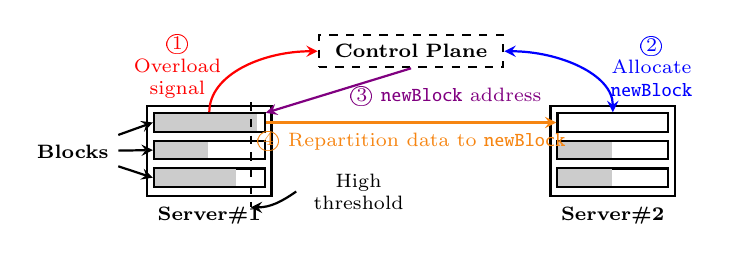
\begin{tikzpicture}[font=\scriptsize, yscale=0.7]
    \node[draw, thick, minimum width=4.5em, minimum height=3.25em] (server1) {};
    \node[draw, thick, minimum width=4em, below=0.25em of server1.north] (block11) {};
    \node[fill=gray!40, minimum width=3.675em, inner sep=3pt] at ([xshift=-0.125em]block11) {};
    \node[draw, thick, minimum width=4em, below=0.25em of block11] (block12) {};
    \node[fill=gray!40, minimum width=1.925em, inner sep=3pt] at ([xshift=-1em]block12) {};
    \node[draw, thick, minimum width=4em, below=0.25em of block12] (block13) {};
    \node[fill=gray!40, minimum width=2.925em, inner sep=3pt] at ([xshift=-.5em]block13) {};
    
    \node[text width=4em, align=center, below=0em of server1] {\textbf{Server\#1}};
    
    \node[left=1em of server1] (block) {\textbf{Blocks}};
    \draw[-stealth, thick] (block) -- (block11.west);
    \draw[-stealth, thick] (block) -- (block12.west);
    \draw[-stealth, thick] (block) -- (block13.west);
    
    \draw[thick, dashed] ($(block11.north)+(1.5em, 0.5em)$) -- ($(block13.south)+(1.5em, -1em)$)node [anchor=north] (ht-line) {};
    
    \node[text width=4.5em, align=center, right=0.75em of block13, yshift=-0.5em] (ht) {High threshold};
    
    \draw[-stealth, thick] ($(ht.west)+(0.35em, 0em)$) to [out=225, in=0] (ht-line.north);
    
    \node[draw, thick, minimum width=4.5em, minimum height=3.25em, right=10em of server1] (server2) {};
    \node[draw, thick, minimum width=4em, below=0.25em of server2.north] (block21) {};
    \node[draw, thick, minimum width=4em, below=0.25em of block21] (block22) {};
    \node[fill=gray!40, minimum width=1.925em, inner sep=3pt] at ([xshift=-1em]block22) {};
    \node[draw, thick, minimum width=4em, below=0.25em of block22] (block23) {};
    \node[fill=gray!40, minimum width=1.925em, inner sep=3pt] at ([xshift=-1em]block23) {};
    
    \node[text width=4em, align=center, below=0em of server2] {\textbf{Server\#2}};
    
    \node[draw, thick, dashed, text width=6em, minimum height=1em, align=center, above=3em of $(server1)!0.5!(server2)$] (cp) {\textbf{Control Plane}};
    
    \draw[thick, color=red, -stealth] (block11.north) to [out=90, in=180] node [left, text width=4em, align=center] {\textcolor{red}{\textcircled{1}} Overload signal} (cp.west);
    
    \draw[thick, color=blue, stealth-stealth] (cp.east) to [out=0, in=90] node [right, text width=4em, xshift=0.25em, align=center] {\textcolor{blue}{\textcircled{2}} Allocate \texttt{newBlock}} (block21.north);
    
    \draw[thick, color=violet, -stealth] (cp.south) -- node [right, text width=7em, align=center, yshift=-0.25em] {\textcolor{violet}{\textcircled{3}} \texttt{newBlock} address} ($(block11.east)+(0em, 0.5em)$);
    
    \draw[thick, color=BurntOrange, -stealth] (block11.east) -- node[midway, below, align=center] {\textcolor{BurntOrange}{\textcircled{4}} Repartition data to \texttt{newBlock}} (block21.west);
  \end{tikzpicture}
  \caption[Data repartitioning on scaling up capacity]{\small\textbf{Data repartitioning on scaling up capacity.} Scaling down capacity employs a similar approach (\S\ref{sec:dp}).}\label{fig:autoscaling}
\end{figure}
%
While the block allocator and metadata manager are similar to their counterparts in Pocket, the lease manager implements lifetime management in \jiffy. It comprises a lease renewal service that listens for renewal requests from jobs and updates the lease renewal timestamp of relevant nodes in its \lh, and a lease expiry worker that periodically traverses all address hierarchies, marking nodes with timestamps older than the associated lease period as expired. Finally, \jiffy adopts mechanisms from Pocket to facilitate control plane scaling and fault tolerance; we refer the reader to~\cite{pocket} for details.

\paragraphb{Data plane} \jiffy data plane is responsible for two main tasks: providing jobs with efficient, data-structure specific atomic access to data, and repartitioning data across blocks allocated by the control plane during resource scaling. It partitions the resources in a pool of storage servers across fixed sized blocks. Each storage server maintains, for the blocks managed by it, a mapping from unique blockIDs to pointers to raw storage allocated to the blocks, along with two additional metadata: data structure-specific operator implementations as described in \S\ref{ssec:jiffyapi}, and a subscription map that maps data structure operations to client handles that have subscribed to receive notifications for that operation. 

Data repartitioning for a \jiffy data structure is implemented as follows: when a block's usage grows above the high threshold, the block sends a signal to the control plane, which, in turn, allocates a new block to the address-prefix and responds to the overloaded block with its location. The overloaded block then repartitions and moves part of its data to the new block (see Figure~\ref{fig:autoscaling}); a similar mechanism is used when the block's usage falls below the low threshold. 

For applications that require fault tolerance and persistence for their intermediate data, \sl supports chain replication~\cite{chainreplication} at block granularity, and synchronously persisting data to external stores (\eg, S3) at address-prefix granularity.


\subsection{Programming Models on \jiffy}
\label{ssec:jiffymodels}

We now describe how \jiffy's built-in data structures (Table~\ref{table:ds}) enable various distributed programming frameworks on serverless platforms (\S\ref{sssec:bsp}-\S\ref{sssec:piccolo}).

\subsubsection{Map-Reduce Model}
\label{sssec:bsp}

A Map-Reduce (MR) program~\cite{mapreduce} consists of map functions that process input key-value (KV) pairs to generate intermediate KV pairs, and reduce functions that merge all intermediate values for the same intermediate key. MR frameworks~\cite{mapreduce, hadoop, spark} parallelize map and reduce functions across multiple workers. Data exchange between map and reduce workers occurs via a shuffle phase, where intermediate KV pairs are distributed to ensure that values with the same key are routed to the same worker.

In \jiffy, MR executes map/reduce tasks as serverless tasks. A master process launches, tracks, and manages task failures across MR jobs. \jiffy stores intermediate KV pairs in multiple shuffle files, each containing a partitioned subset of KV pairs from all map tasks. Since multiple map tasks may write to the same shuffle file, \jiffy's strong consistency semantics ensure correctness. The master process also handles explicit lease renewals. We now describe \jiffy files in more detail.

\paragraphb{\jiffy Files} A \jiffy file consists of multiple blocks, each storing a fixed-sized chunk of the file. The controller manages the mapping between blocks and file offset ranges at the metadata manager, and clients cache this mapping when accessing the file. The mapping is updated whenever the number of blocks allocated to the file scales. The \texttt{getBlock} operator forwards requests to the correct file block based on the request's offset range. Files support sequential \texttt{read}s and append-only \texttt{write}s. For random access, files support \texttt{seek} with arbitrary offsets, using the offset to locate the corresponding block. Since files are append-only, blocks are only added and do not require repartitioning when new blocks are added.

\subsubsection{Dataflow and Streaming Dataflow Models}
\label{sssec:dflow}

In the dataflow model, applications describe their communication patterns using directed acyclic graphs (DAGs), where DAG vertices represent computations, and data channels form directed edges between them. We refer to Dryad~\cite{dryad} as a reference dataflow execution engine, where channels can be files, shared memory FIFO queues, etc. The Dryad runtime schedules DAG vertices based on their dataflow dependencies: a vertex is scheduled once all its input channels are ready. A file channel is ready if its data has been fully written, while a queue is ready if it contains any data. Streaming dataflow~\cite{streamscope} adopts a similar approach but operates on continuous event streams.

On \jiffy, each DAG vertex corresponds to a serverless task, with a master process managing vertex scheduling, fault tolerance, and lease renewals. \jiffy uses FIFO queues and files as data channels. Queue-based channels are considered ready as long as a vertex is writing to them, and \jiffy allows downstream tasks to efficiently detect item availability via notifications, described below.

\paragraphb{\jiffy Queues} The FIFO queue in \jiffy is implemented as a growing linked-list of blocks, each storing multiple data items and a pointer to the next block. Queue size can be limited by setting a \texttt{maxQueueLength}. The controller manages only the head and tail blocks of the queue, and clients cache and update this information when blocks are added or removed. The FIFO queue supports \texttt{enqueue} and \texttt{dequeue} operations for adding and removing items. The \texttt{getBlock} operator routes these operations to the current tail and head blocks, respectively. Unlike other structures, queues do not require repartitioning. The FIFO queue uses \jiffy’s notification system to asynchronously detect when there is space to add items or when data is available for consumption through subscriptions to \texttt{enqueue} and \texttt{dequeue} events.

\subsubsection{Piccolo}
\label{sssec:piccolo}

Piccolo~\cite{piccolo} is a data-centric programming model that allows distributed machines to share mutable state. Piccolo kernel functions define sequential application logic, while sharing state with concurrent kernel functions via a KV interface. Centralized control functions create and coordinate both shared KV stores and kernel instances. Concurrent updates to the same key are resolved using user-defined accumulators.

On \jiffy, Piccolo kernel functions execute across serverless tasks, while control tasks run on a centralized master. Shared state is stored in \jiffy’s KV-store data structures (described below), which may be created per kernel function or shared across multiple functions as needed. The master periodically renews leases for \jiffy KV-stores, and, like Piccolo, \jiffy checkpoints KV-stores by flushing them to external storage.

\paragraphb{\jiffy KV-store} The \jiffy KV-store hashes each key into one of $H$ hash slots, where $H = 1024$ by default. The KV-store shards KV pairs across multiple \jiffy blocks, with each block responsible for one or more hash slots. A hash slot is fully contained within a single block. The controller manages the mapping between blocks and their corresponding hash slots, and this mapping is cached at the client and updated during scaling. Each block stores KV pairs as a hash table. The KV-store supports standard \texttt{get}, \texttt{put}, and \texttt{delete} operations via \texttt{readOp}, \texttt{writeOp}, and \texttt{deleteOp} operators. The \texttt{getBlock} operator routes requests to blocks based on key hashes.

Unlike files and queues, the KV-store requires repartitioning when blocks are added or removed. When a block becomes nearly full, \jiffy splits half of its hash slots into a new block, moves the relevant KV pairs, and updates the mapping at the controller. Similarly, when a block is underutilized, its hash slots are merged with another block.




\section{Evaluation}
\label{sec:jiffyevaluation}
\jiffy is implemented in 25K lines of C++, with client libraries in C++, Python, and Java (each around 1K LOC), in addition to the original Pocket codebase. In this section, we evaluate \jiffy to showcase its benefits (\S\ref{ssec:overallbenefits}, \S\ref{ssec:hrelated}) and analyze the contributions of individual \jiffy mechanisms to overall performance (\S\ref{ssec:overallbenefits}). Lastly, we assess \jiffy’s controller overheads in \S\ref{ssec:controller-scale}.

\paragraphb{Experimental setup} Unless specified otherwise, each intermediate storage system in our experiments is deployed across 10 m4.16xlarge EC2~\cite{ec2} instances, while serverless applications are hosted on AWS Lambda~\cite{ec2}. Since \jiffy builds on Pocket's design, it supports adding new instances to increase overall system capacity. However, our experiments do not evaluate the overheads of scaling system capacity, as this is orthogonal to \jiffy’s focus. Instead, we concentrate on multiplexing the available storage capacity for higher utilization, reducing the need to add more resources. \jiffy employs 128MB blocks, a 1-second lease duration, and thresholds of 5\% (low) and 95\% (high) for data repartitioning.

\begin{figure}[t]
  \centering
  \subfigure[Job performance] {
    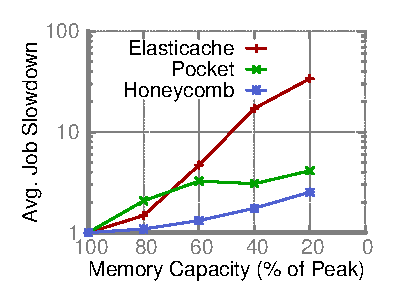
\includegraphics[width = 0.4\textwidth]{fig/jiffy/perfvcap}
    \label{fig:perfvcap}
  }
  \subfigure[Resource utilization] {
    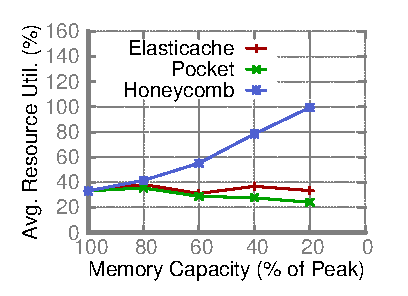
\includegraphics[width = 0.4\textwidth]{fig/jiffy/utilvcap}
    \label{fig:utilization}
  }
  \caption[Fine-grained task-level elasticity in \jiffy]{\textbf{Fine-grained task-level elasticity in \jiffy} enables (a) better job performance, and (b) higher resource utilization under constrained capacity. In (a), the slowdown is computed relative to the job completion time with $100\%$ capacity (for this data point, Elasticache performance was $30\%$ worse than Pocket, and Pocket performance was $5\%$ worse than \jiffy). See \S\ref{ssec:overallbenefits} for details.}
  \label{fig:elasticity}\vspace{-1.25em}
\end{figure}


\subsection{Benefits of \jiffy}
\label{ssec:overallbenefits}

\jiffy enables fine-grained resource allocation for serverless analytics. We demonstrate its impact on job performance and resource utilization across approximately 50,000 jobs from 100 randomly selected tenants over a 5-hour window in the Snowflake workload\footnote{We did not evaluate the full 14-day window with $>2000$ tenants due to intractable cost overheads.}~\cite{snowset}.

We compare \jiffy (using the MR programming model, \S\ref{ssec:jiffymodels}) with Elasticache~\cite{elasticache} and Pocket~\cite{pocket}. Elasticache provisions resources for \textit{all} jobs, and if capacity is insufficient, jobs must spill data to external stores like S3~\cite{s3}. Pocket, however, reserves and reclaims resources at a \textit{job} granularity, spilling data to SSD if DRAM capacity is insufficient. Pocket’s utilization can be lower than Elasticache, as it provisions separately for the peak demand of each job, which sacrifices overall utilization. To ensure a fair comparison, Pocket’s control and metadata services are colocated on the same server, similar to \jiffy’s unified control plane.

\paragraphb{Impact of fine-grained elasticity on job performance} We examine job performance under constrained intermediate storage capacity in the Snowflake workload. Figure~\ref{fig:perfvcap} shows the average job slowdown as capacity is reduced to a fraction of peak utilization. With Elasticache, performance drops sharply when data exceeds capacity, leading to a $34\times$ slowdown at 20\% capacity due to reliance on S3. Pocket experiences a $>4.1\times$ slowdown at 20\% capacity as it spills data to SSD. In contrast, \jiffy’s task-level elasticity and lease-based storage reclamation reduce data spilling, resulting in a much lower slowdown ($<2.5\times$ at 20\% capacity). This is because \jiffy multiplexes capacity more efficiently across jobs, minimizing reliance on slower storage tiers.

\paragraphb{Impact of fine-grained elasticity on resource utilization} Figure~\ref{fig:utilization} shows resource utilization under constrained capacity. While Elasticache and Pocket see reduced or stagnant utilization as capacity is constrained, \jiffy’s utilization \textit{improves}. Elasticache and Pocket allocate capacity at a job or coarser granularity, wasting unused resources regardless of total system capacity. In contrast, \jiffy’s fine-grained elasticity and lease-based reclamation allow it to multiplex capacity more effectively, reducing SSD spillover and improving performance as shown in Figure~\ref{fig:perfvcap}.


\begin{figure}
  \centering
  \subfigure[Latency] {
    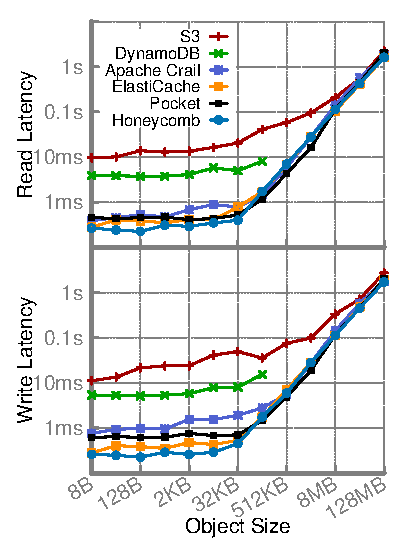
\includegraphics[width = 0.4\textwidth]{fig/jiffy/rw_latency}
    \label{fig:rwlatency}
  }%
  \subfigure[MBPS] {
    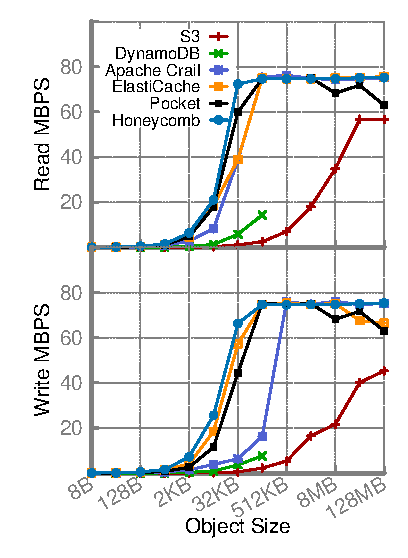
\includegraphics[width = 0.4\textwidth]{fig/jiffy/rw_mbps}
    \label{fig:rwmbps}
  }%
  \caption[\jiffy performance comparison with existing storage systems]{\small{\textbf{\jiffy performance comparison with existing storage systems (\S\ref{ssec:hrelated}).} Despite providing the additional benefits demonstrated in \S\ref{ssec:overallbenefits}, \jiffy performs as well as or outperforms state-of-the-art storage systems for serverless analytics.}}
  \label{fig:storage-perf}
\end{figure}

\subsection{Performance Benchmarks for Six Systems}
\label{ssec:hrelated}

We now compare \jiffy’s performance (using its KV-Store data structure) against five state-of-the-art systems commonly used for intermediate data storage in serverless analytics: S3, DynamoDB, Elasticache, Apache Crail, and Pocket. Since only a subset of these systems support request pipelining, we disable pipelining across all of them for consistency.

To measure latency and throughput, we profiled synchronous operations issued from an AWS Lambda instance using a single-threaded client. Figure~\ref{fig:storage-perf} shows that in-memory data stores like Elasticache, Pocket, and Apache Crail achieve low latency (sub-millisecond) and high throughput. In contrast, persistent data stores like S3 and DynamoDB exhibit significantly higher latencies and lower throughput; note that DynamoDB only supports objects up to $128$KB. \jiffy matches the performance of these in-memory data stores while also providing the additional benefits discussed in \S\ref{ssec:overallbenefits}.


\begin{figure*}[t]
  \centering
  \subfigure[Efficient lifetime management] {
    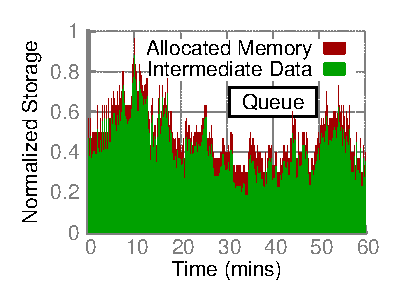
\includegraphics[width = 0.3\textwidth]{fig/jiffy/fifo_queue_scale_uniform}\hspace{-.5em}%
    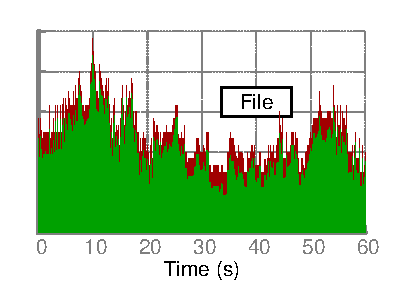
\includegraphics[width = 0.3\textwidth]{fig/jiffy/file_scale_uniform}\hspace{-.5em}%
    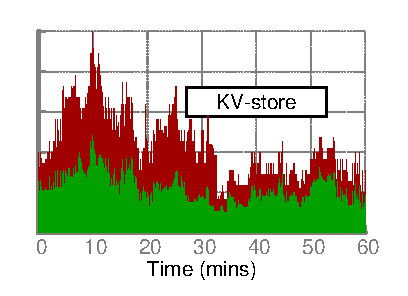
\includegraphics[width = 0.3\textwidth]{fig/jiffy/scale_zipf}
    \label{fig:fi-scale}
    \label{fig:ht-scale}
    \label{fig:fq-scale}
  }\\
  \subfigure[Efficient data repartitioning] {
    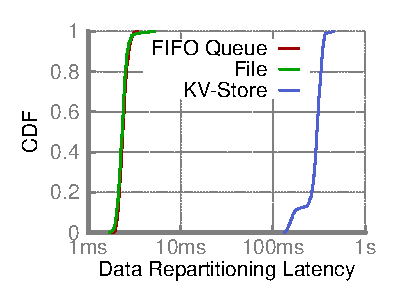
\includegraphics[width = 0.3\textwidth]{fig/jiffy/scale_latency_cdf}\hspace{-1.5em}%
    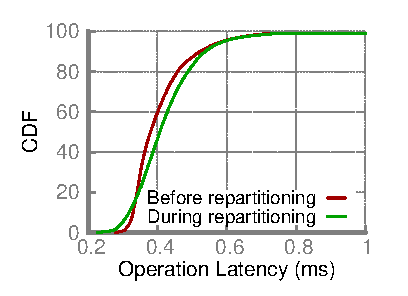
\includegraphics[width = 0.3\textwidth]{fig/jiffy/hash_table_scaling_get}
    \label{fig:op-latency-scaling}
    \label{fig:scale-latency}
  }
  \caption[\jiffy data lifetime-management and data repartitioning]{\textbf{\jiffy data lifetime-management and data repartitioning.} (a) \jiffy provides fine-grained elasticity through lease-based lifetime management for its built-in data structures: FIFO Queue (left), File (center), and KV-store (right). It efficiently reclaims resources from tasks once their leases expire. (b) \jiffy enables efficient data repartitioning as allocations scale up, with repartitioning for a single block completing within $2$-$500$ms (left). Additionally, the latency for 100KB \texttt{get} operations is minimally affected during KV-store repartitioning. Note: plots in (a) and (b) share a common y-axis; the x-axis for (c, left) is in log scale.}
\end{figure*}


\subsection{Understanding \jiffy Benefits}
\label{ssec:jiffybenefits}

Figure~\ref{fig:elasticity} demonstrates how \jiffy's fine-grained elasticity provides performance and resource utilization advantages over other state-of-the-art systems. This elasticity is achieved through hierarchical virtual addressing, flexible data lifetime management, and data repartitioning. In this section, we isolate and evaluate the impact of these mechanisms.

\paragraphb{Fine-grained elasticity via data lifetime management} Unlike traditional storage systems, \jiffy’s lease-based data lifetime management enables the reclamation of unused resources, reallocating them to jobs in need. Coupled with fine-grained resource allocations and efficient data repartitioning, this enables elasticity for serverless jobs. To evaluate this, we examine storage allocation across various \jiffy data structures (Figure~\ref{fig:fq-scale}) using the Snowflake workload from Figure~\ref{fig:ephemerals}.

FIFO queue and file data structures exhibit seamless elasticity as intermediate data is written to them, as they do not require repartitioning. The allocated capacity slightly exceeds the intermediate data size, accounting for block metadata (e.g., object metadata for FIFO queue items) and unused space in head/tail blocks. For the KV-store, inserted keys are sampled from a Zipf distribution since the Snowflake dataset lacks access patterns. Due to the skew, some \jiffy blocks receive most key-value pairs and frequently split when their capacity grows too high, leading to higher allocated capacity. However, \jiffy’s lease mechanism quickly reclaims resources after their utility ends, ensuring that overheads are temporary.

\paragraphb{Efficient elastic scaling via flexible data repartitioning} A key factor in \jiffy’s elasticity is its efficient data repartitioning. Figure~\ref{fig:scale-latency} shows the CDF of repartitioning latency per block across the three data structures under the Snowflake workload. The latency includes the time from detecting an overloaded/underloaded block to the completion of repartitioning. Storage servers take ${\sim}1$-$1.5$ms to connect to the controller, with two round trips ($100$-$200\mu$s in EC2) to trigger block allocation/reclamation and update partitioning metadata. Unlike FIFO Queue and File, KV-Store requires data repartitioning across blocks, but since only half the block capacity (${\sim}64$MB) is moved, \jiffy completes repartitioning in a few hundred milliseconds over $10$Gbps links, achieving block-level repartitioning with low latency ($2$-$500$ms).

Importantly, \jiffy does not block data structure operations during repartitioning. As shown in Figure~\ref{fig:op-latency-scaling}, the CDF of 100KB \texttt{get} operations in the KV-Store before and during scaling remains almost identical, indicating minimal impact on operation latency during scaling.


\begin{figure}[h]
  \centering
  \subfigure[Controller throughput vs. latency on a single CPU core.] { 
    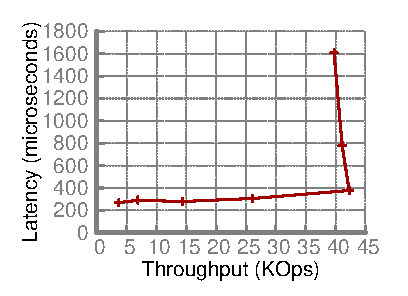
\includegraphics[width = 0.4\textwidth]{fig/jiffy/controller_tvl}
    \label{fig:controller-tvl}
  }
  \subfigure[Controller throughput scaling with multiple cores.] {
    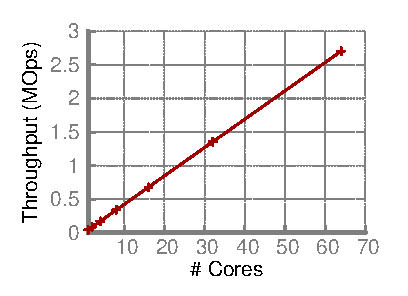
\includegraphics[width = 0.4\textwidth]{fig/jiffy/controller_scale}
    \label{fig:controller-scaling}
  }
  \caption[\jiffy controller performance]{{\textbf{\jiffy controller performance.} Details in Appendix~\ref{ssec:controller-scale}.}}
  \label{fig:controller-perf}
\end{figure}

\subsection{Controller Overheads}
\label{ssec:controller-scale}

\jiffy introduces several additional components at the controller compared to Pocket, including metadata management, lease management, and handling data repartitioning requests. As a result, its performance is expected to be lower than Pocket's metadata server. However, this is acceptable as long as \jiffy can manage the typical control plane request rates observed in real-world workloads, such as the peak of a few hundred requests per second—including lease renewals—seen in our evaluations and those in~\cite{pocket}.

Figure~\ref{fig:controller-tvl} shows the throughput-versus-latency curve for \jiffy controller operations on a single CPU core of an m4.16xlarge EC2 instance. The controller throughput saturates at around $42$ KOps with a latency of $370\mu$s. While this is lower than Pocket's throughput (~$90$ KOps per core), it is more than sufficient to handle the control plane load of real-world workloads. Additionally, throughput scales almost linearly with the number of cores, as each core processes requests independently for distinct subsets of virtual address hierarchies (Figure~\ref{fig:controller-scaling}). Finally, the control plane can scale across multiple servers by partitioning the address hierarchies.

\paragraphb{Storage overheads} The task-level metadata storage in Honeycomb has a minimal overhead of just 64 bytes of fixed metadata per task and 8 bytes per block. For \jiffy's default 128MB blocks, this results in an insignificant storage overhead ($<0.00005-0.0001\%$ of total storage).


\begin{figure*}[t]
  \centering
  \subfigure[Sensitivity analysis for block size] {
    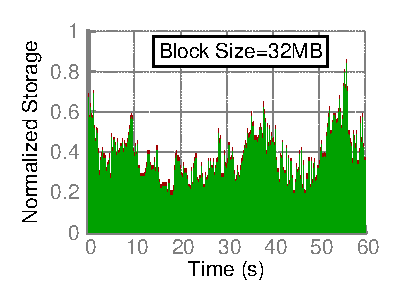
\includegraphics[width = 0.25\textwidth]{fig/jiffy/block_size_32}\hspace{-.5em}%
    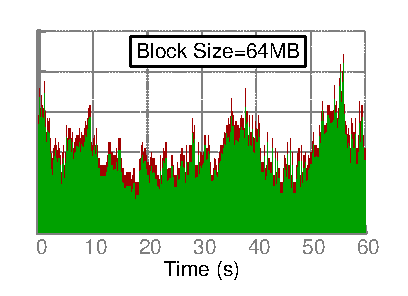
\includegraphics[width = 0.25\textwidth]{fig/jiffy/block_size_64}\hspace{-.5em}%
    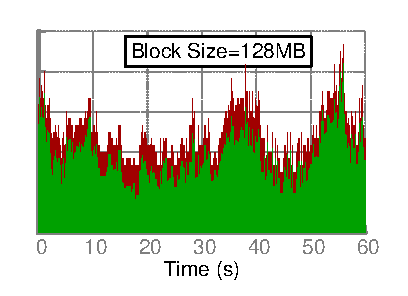
\includegraphics[width = 0.25\textwidth]{fig/jiffy/block_size_128}\hspace{-.5em}%
    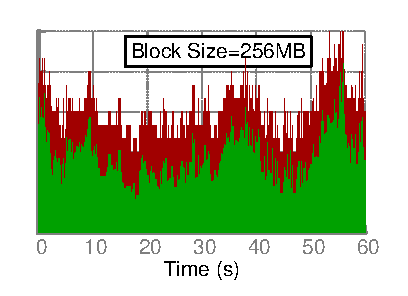
\includegraphics[width = 0.25\textwidth]{fig/jiffy/block_size_256}\hspace{-.5em}%
    %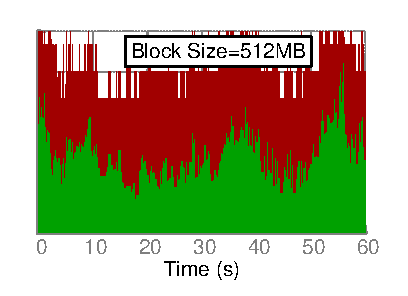
\includegraphics[width = 1.4in]{fig/jiffy/block_size_512}
    \label{fig:block-size}
  }
  \subfigure[Sensitivity analysis for lease duration] {
    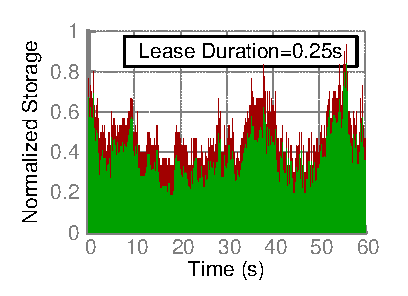
\includegraphics[width = 0.25\textwidth]{fig/jiffy/lease_duration_0_25}\hspace{-.5em}%
    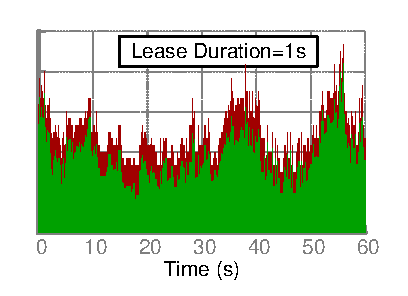
\includegraphics[width = 0.25\textwidth]{fig/jiffy/lease_duration_1}\hspace{-.5em}%
    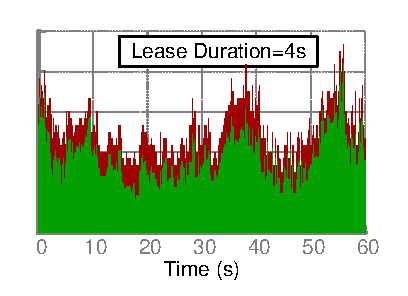
\includegraphics[width = 0.25\textwidth]{fig/jiffy/lease_duration_4}\hspace{-.5em}%
    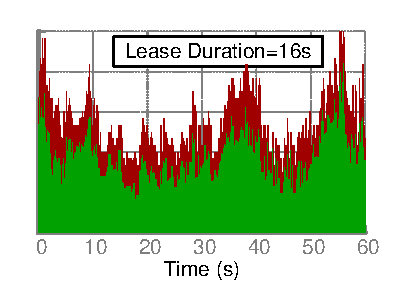
\includegraphics[width = 0.25\textwidth]{fig/jiffy/lease_duration_16}\hspace{-.5em}%
    %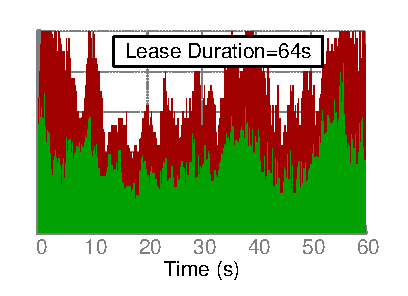
\includegraphics[width = 1.4in]{fig/jiffy/lease_duration_64}
    \label{fig:lease-duration}
  }
  \subfigure[Sensitivity analysis for (high) repartition threshold] {
    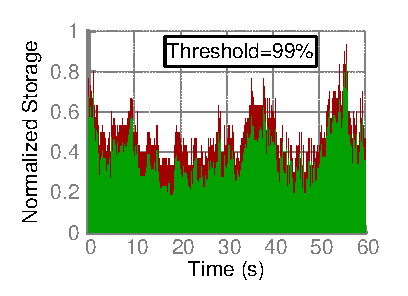
\includegraphics[width = 0.25\textwidth]{fig/jiffy/threshold_0_99}\hspace{-.5em}%
    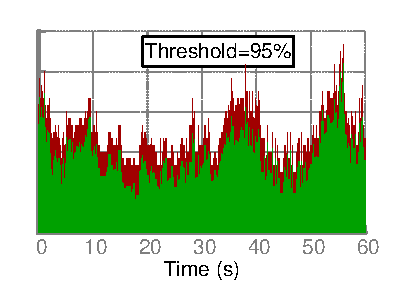
\includegraphics[width = 0.25\textwidth]{fig/jiffy/threshold_0_95}\hspace{-.5em}%
    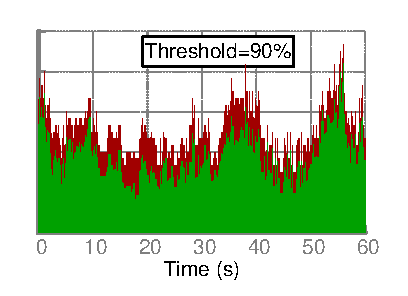
\includegraphics[width = 0.25\textwidth]{fig/jiffy/threshold_0_9}\hspace{-.5em}%
    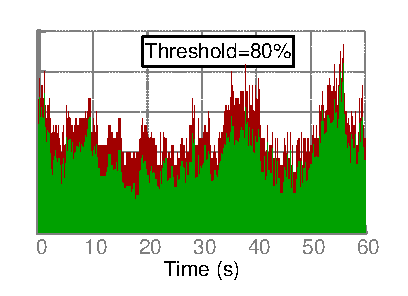
\includegraphics[width = 0.25\textwidth]{fig/jiffy/threshold_0_8}\hspace{-.5em}%
    %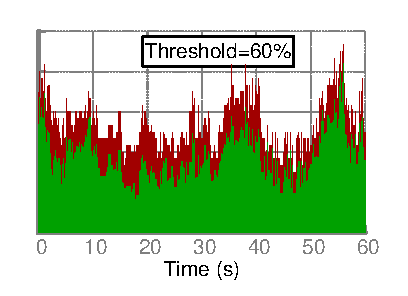
\includegraphics[width = 1.4in]{fig/jiffy/threshold_0_6}
    \label{fig:threshold}
  }
  \caption[\jiffy sensitivity analysis]{\textbf{\jiffy sensitivity analysis} for (a) block size (b) lease duration and (c) repartition threshold for the file data structure. Green area corresponds to used capacity, while red area corresponds to allocated capacity under \jiffy. See Appendix~\ref{ssec:jiffysensitivity} for details.}
\end{figure*}


\subsection{Sensitivity Analysis}
\label{ssec:jiffysensitivity}

We now perform sensitivity analysis for various system parameters in \jiffy, including block size (\S\ref{ssec:hva}), lease duration (\S\ref{ssec:mlm}) and thresholds for data repartitioning (\S\ref{ssec:fdr}). We use files as our underlying data structure, and use the Snowflake workload from Figure~\ref{fig:ephemerals}. These results can be contrasted directly with Figure~\ref{fig:fi-scale}~(center), which corresponds to our default system parameters ($128$MB blocks, $1$s lease duration and $95\%$ of block occupancy as repartition threshold). For each parameter that we vary, the other to remain fixed at their default values.

\paragraphb{Block size (Figure~\ref{fig:block-size})} As discussed in \S\ref{ssec:hva}, the block size in \jiffy exposes a tradeoff between the amount of metadata that needs to be stored at the control plane, and resource utilization. This is confirmed in Figure~\ref{fig:block-size}, where increasing the block size from $32$MB to $256$MB increases the disparity between allocated and used capacity, and therefore decreases the resource utilization. The default block size in \jiffy is set to $128$MB for two main reasons: (1) it allows high enough utilization with low enough metadata overhead (a few megabytes for even thousands of gigabytes of application data), and (2) it is the default block size used in existing data analytics platforms; as such, $128$MB blocks ensure seamless compatibility with such frameworks.

\paragraphb{Lease duration (Figure~\ref{fig:lease-duration})} As shown in Figure~\ref{fig:lease-duration}, lease duration in \jiffy controls resource utilization over time. As we increase lease durations from $0.25$ seconds to $16$ seconds, resource utilization increases since \jiffy does not reclaim (potentially unused) resource resources from jobs until their leases expire. At the same time, if we keep lease duration too low, applications would renew leases too often, resulting in higher traffic to the \jiffy controller. We find a lease duration of $1$s to be a sweet spot, ensuring high enough resource utilization, while ensuring the number of lease requests for even thousands of concurrent applications is only a few thousand requests per second --- well within \jiffy controller's limits on a single CPU core.

\paragraphb{Repartition threshold (Figure~\ref{fig:threshold})} Finally, Figure~\ref{fig:threshold} shows the impact of (high) repartition threshold on resource utilization. As expected, lowering the repartition threshold leads to poor utilization, since it triggers pre-mature allocation of new blocks to most files in our evaluated workload. However, since the size of the block ($128$MB) is much smaller than the amount of data written to each file in the workload (often several gigabytes), this overhead is relatively small when compared to effect of other parameters. However, a larger value of high repartitioning threshold results in more frequent block allocation requests to the controller; we find that our default value of $95\%$ provides a reasonable compromise between resource utilization and number of control plane requests.


\section{Related Work}
Pocket~\cite{pocket} demonstrates how existing designs for in-memory key-value stores~\cite{redis, farm, memcached, memc3, mica, ramcloud, anna, succinct, blowfish}, distributed~\cite{dsm1, dsm2, dsm3, treadmarks}, and disaggregated memory systems~\cite{infiniswap,remoteregions,legoos,mind}, as well as storage systems with flexible interfaces~\cite{udf1, udf2, udf3, storedprocedure1, storedprocedure2, storedprocedure3, boxwood, sinfonia}, can be adapted to achieve three primary goals for intermediate data storage in serverless analytics: low-latency/high-throughput, resource sharing, and elasticity.

Other recent systems have also explored fine-grained resource sharing. Pisces~\cite{pisces} provides per-tenant performance isolation in multi-tenant cloud storage systems but does not share storage capacity across tenants. Memshare~\cite{memshare} facilitates memory sharing across tenants in a KV cache setting, though it evicts KV pairs with lower contribution to hit-rate under high contention.


\section{Summary}
\label{sec:jiffysummary}
In this chapter, we have presented \jiffy, a memory management service designed for disaggregated memory, allocating memory in small fixed-size blocks. These blocks store intermediate data for individual tasks within a job. Inspired by virtual memory systems in operating systems, \jiffy scales memory resources elastically without prior knowledge of data sizes, adapting to job demands in real-time. This approach allows \jiffy to efficiently share fast memory across jobs, reducing reliance on slower secondary storage such as S3.









\chapter{Operating System Layer: In-network Near-Memory Processing}
\label{chap:os}
In the previous chapter, we examined the design of memory management for disaggregated architectures at the service layer. However, integrating general-purpose applications (beyond serverless data analytics) with an external memory service (e.g., Jiffy) often necessitates significant code rewrites to accommodate its API, which may be an undesirable burden for application developers. In this chapter, we shift focus to the potential of embedding memory management functionality directly within the operating system (OS). By enabling the OS to handle memory management transparently, existing data center applications can be seamlessly transitioned to a disaggregated architecture, allowing them to benefit from the high resource utilization and efficiency that such architectures provide.

\section{Background: In-network OS design}

Despite the increased interest in memory disaggregation from both academia~\cite{memdisagg2, memdisagg3, memdisagg4, memdisagg5, memdisagg6, memdisagg1, legoos, infiniswap, fastswap, disagg, disaggfault} and industry~\cite{industry0, industry1, industry2, industry3, industry4, industry5}, memory disaggregation still faces three major challenges. First, remote memory access must have low latency and high throughput, with targets of $10~\mu$s latency and $100$ Gbps bandwidth per compute blade~\cite{legoos, infiniswap, fastswap, disagg}. Second, both compute and memory resources need to scale elastically. Finally, adoption requires support for unmodified applications.

We present \mind, the first memory management system for rack-scale disaggregated memory that addresses these challenges by placing the \mmm within the network fabric, leveraging programmable network switches~\cite{progswitch1, progswitch2}.

%To achieve this, \mind introduces:
%\begin{itemize}
%  \item \textbf{Global Virtual Address Space}: A range-partitioned virtual address space across memory blades to minimize address translation overhead.
%  \item \textbf{Domain-Based Memory Protection}: Decouples permissions from address translation, allowing flexible protection with minimal switch memory overhead.
%  \item \textbf{Directory-Based Cache Coherence}: Adapts MSI coherence~\cite{msi} using switch ASIC multicast to minimize network overhead.
%  \item \textbf{Dynamic Memory Region Sizing}: Adjusts memory region sizes dynamically, balancing performance and storage efficiency.
%\end{itemize}

\begin{table}
    \caption[Parallels between memory \& networking primitives]{\small \textbf{Parallels between memory \& networking primitives.}}
    \label{table:isomorph}
    \centering
    \scriptsize
    \renewcommand{\arraystretch}{1.2}
    \begin{tabular}{p{3cm} p{1cm}p{3cm}}
      \hline
      \textbf{Virtual Memory} &$\Longleftrightarrow$ &\textbf{Networking} \\\hline\hline
      Memory allocation&&IP assignment\\
      Address translation &&IP forwarding\\
      Memory protection  &&Access control\\
      Cache invalidations &&Multicast\\
      \hline
    \end{tabular}
\end{table}


\begin{figure*}[!t]
\centering
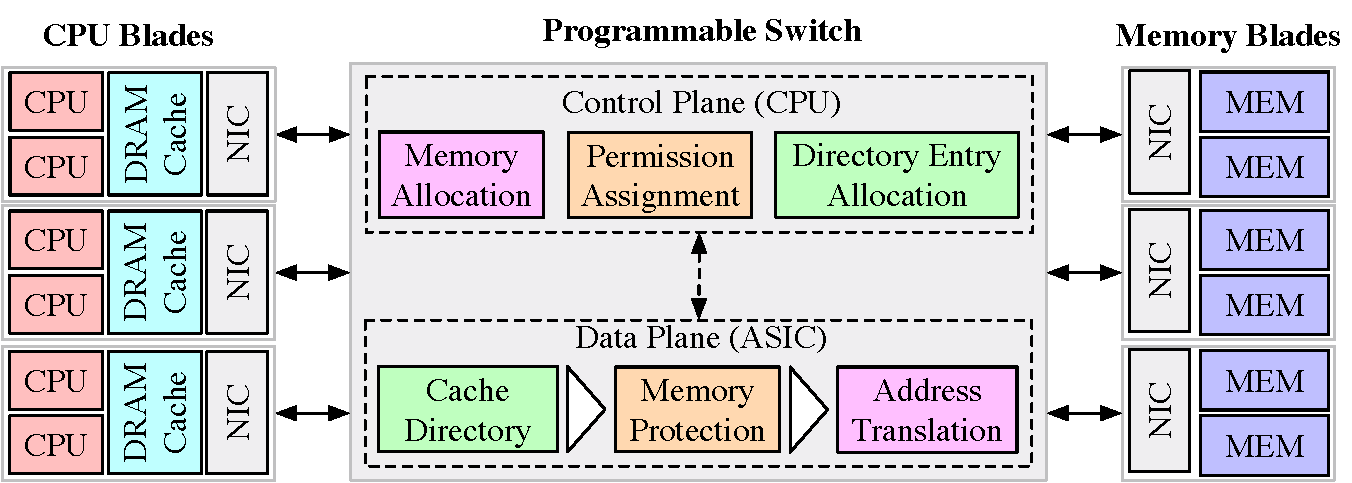
\includegraphics[width=0.55\textwidth]{fig/mind/design}\hspace{3em}
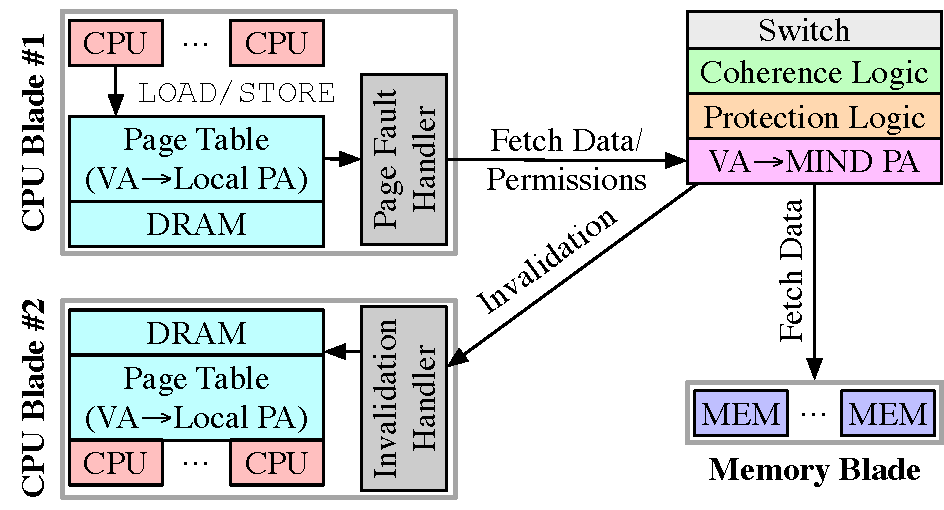
\includegraphics[width=0.35\textwidth]{fig/mind/data_flow}%\vspace{-1em}
\vspace{-0.5em}
\caption[High-level \mind architecture and data flow for memory accesses in \mind]{\textbf{(left) High-level \mind architecture, and, (right) data flow for memory accesses in \mind.}}
\label{fig:system_diagram}
\end{figure*}

\mind places memory management \textit{in the network fabric} for three key reasons: (1) its central location and global view allow direct memory access without metadata coherence, (2) modern programmable network switches~\cite{progswitch1} execute at line rate, which is a good target for implementing the memory management logic, and (3) placing cache coherence logic in the network reduces latency and bandwidth overhead. 

\mind exposes a \textit{transparent virtual memory} abstraction to applications, similar to traditional OSes. It intercepts memory allocations at CPU blades and performs memory operations via RDMA, leveraging a switch-based MMU for cache coherence. Memory blades store pages and serve RDMA requests directly, enabling true hardware disaggregation. Figure~\ref{fig:system_diagram}(left) shows an overview of \mind's design, while Figure\ref{fig:system_diagram}~(right) illustrates its memory access flow. CPU blades run user processes and use local DRAM as a cache. Memory allocations and deallocations are intercepted and forwarded to the switch control plane, which manages allocations and permissions. All memory operations are handled by the CPU cache, with virtual addresses translated locally. If a page is not cached, a page fault triggers RDMA to fetch it from memory blades. Coherence updates also trigger page faults, handled by the switch.Since the CPU blade lacks memory metadata, RDMA requests only use virtual addresses. The switch data plane intercepts them, handling cache coherence, permission checks, and address translation. If no cache holds the page, it forwards the request to the correct memory blade. \mind relies on one-sided RDMA, eliminating the need for CPUs on memory blades, moving towards full hardware disaggregation.


%\section{In-Network Memory Management}
\label{sec:mindintro}

Data center network bandwidth is approaching that of intra-server resource interconnects~\cite{terabitethernet, remotememory}, and is soon poised to surpass it~\cite{legoosatc}. This has driven significant academic~\cite{memdisagg2, memdisagg3, memdisagg4, memdisagg5, memdisagg6, memdisagg1, legoos, infiniswap, fastswap, disagg, disaggfault} and industry~\cite{industry0, industry1, industry2, industry3, industry4, industry5} interest in memory disaggregation, where compute and memory are physically separated into network-attached \textit{resource blades}, drastically improving resource utilization, hardware heterogeneity, resource elasticity and failure handling compared to traditional data center architectures. 

However, memory disaggregation is challenging due to three requirements. First,  access to remote memory must have low latency and high throughput --- prior work~\cite{legoos, infiniswap, fastswap, disagg} have targeted $10~\mu$s latency and $100$~Gbps bandwidth per compute blade to minimize application performance degradation. Second,  both memory and compute resources available to applications must scale elastically, in keeping with the promise of disaggregation. Finally, wide adoption and immediate deployment requires support for unmodified applications.

Despite years of research towards enabling memory disaggregation, none of the known approaches support all three requirements simultaneously (\S\ref{ssec:challenges}). Most approaches require application modifications due to changes in hardware~\cite{industry1, industry2, nwsupport, memdisagg4}, programming model~\cite{piccolo, grappa}, or memory interface~\cite{farm, ramcloud, herd}. Recent approaches that enable transparent access to disaggregated memory~\cite{legoos, infiniswap, fastswap} limit application compute elasticity --- processes are limited to compute resources on a single compute blade to avoid cache coherence traffic over the network due to performance concerns.

We present \mind, the first memory management system for rack-scale memory disaggregation that simultaneously meets all three requirements for disaggregated memory. Our key idea is to place the \mmm \textit{in the network fabric}. \mind's design builds on the observation that the network fabric in the disaggregated memory architecture is essentially a CPU-memory interconnect. In \mind, centrally-placed in-network processing devices like programmable network switches~\cite{progswitch1, progswitch2, progswitch3} therefore assume the role of the MMU to enable a high-performance shared memory abstraction. Since \mind realizes the \mmm in programmable hardware at line rate~\cite{progswitch1}, latency and bandwidth overheads are minimal. 

Realizing in-network memory management, however, requires working with the unique constraints imposed by programmable switch ASICs. First, today's switch ASICs only have a few megabytes of on-chip memory, making it challenging to store traditional page tables for potentially terabytes of disaggregated memory. Second, switch ASICs only permit a few cycles of limited computations per packet to ensure line-rate processing, while cache coherence may require complex state transition logic for each cached block. Finally, these ASICs~\cite{p4paper} have staged packet processing pipelines where compute and memory resources are spread across multiple physically decoupled match-action stages, introducing interesting challenges in partitioning and placing the \mmm across them. 

To meet the three requirements of memory disaggregation, \mind effectively navigates the above constraints and explores the capabilities of today's programmable switches to enable in-network memory management for disaggregated architectures. It does so through a principled redesign of traditional memory management:
\begin{itemize}[leftmargin=*, itemsep=0pt]
  \item \mind employs a \textit{global virtual address space} shared by all processes, range partitioned across memory blades to minimize the number of address translation entries that need to be stored in the on-chip memory of switch ASIC. At the same time, it employs a physical memory allocation mechanism that load balances allocations across memory blades for high memory throughput (\S\ref{subsec:addr_trans}).
  \item \mind features domain-based memory protection inspired by capability-based schemes~\cite{capabilityaddr, cap, opal} that enables fine-grained and flexible protection by decoupling the storage of memory permissions from address translation entries. Interestingly, such a decoupling actually \textit{reduces} the on-chip memory overheads at the switch ASIC (\S\ref{subsec:mem_prot}).
  \item \mind adapts directory-based MSI coherence~\cite{msi} to the in-network setting. To mitigate the network overheads of cache coherence, \mind exploits network-centric hardware primitives such as multicast in the switch ASIC to efficiently realize its coherence protocol (\S\ref{ssec:caching}).
  \item We find that the limited on-chip memory at the switch ASIC forces the cache directory to track memory regions at coarse granularities, which in turn results in performance degradation due to \textit{false invalidations} of pages in those regions (\S\ref{ssec:caching}). We address this through a novel \sizing algorithm (\S\ref{sec:algorithm}) that dynamically sizes memory regions to bound both the switch storage requirements as well as performance overheads due to false invalidations.
\end{itemize}
\noindent
We realize \mind design on a disaggregated cluster emulated using traditional servers connected by a programmable switch. Our results show that \mind enables transparent resource elasticity for real-world workloads while matching the performance for prior memory disaggregation proposals (\S\ref{sec:evaluation}). 

We also find that while \mind is competitive with compared systems, workloads with high read-write contention experience sub-linear scaling with more threads due to limitations of current hardware. Current x86 architectures preclude realization of relaxed consistency models commonly employed in shared memory systems~\cite{gam}, and the switch TCAM capacity is close to saturated with cache directory entries for such workloads. We discuss approaches that could enable better scaling with future improvements in switch ASIC and compute blade architectures in \S\ref{sec:discussion}.


This section motivates \mind. We discuss key enabling technologies (\S\ref{ssec:assumptions}), followed by challenges in realizing memory disaggregation goals using existing designs (\S\ref{ssec:challenges}).

\paragraphb{Assumptions} We focus on memory disaggregation at the \textit{rack-scale}, where memory and compute blades are connected by a single programmable switch. Similar to prior work~\cite{memdisagg2, memdisagg3, memdisagg4, memdisagg5, memdisagg6, memdisagg1, legoos, disagg}, we restrict our scope to \textit{partial} memory disaggregation: while most of the memory is network-attached, CPU blades possess a small amount (few GBs) of local DRAM as cache.

\begin{figure}[t]
  \centering
  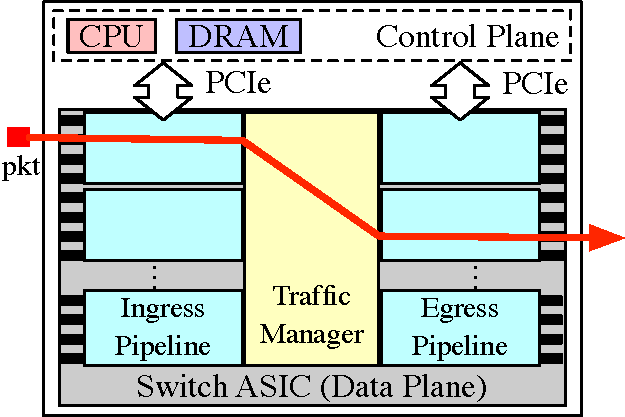
\includegraphics[width=0.44\columnwidth]{fig/mind/prog-switch.pdf}\hfill
  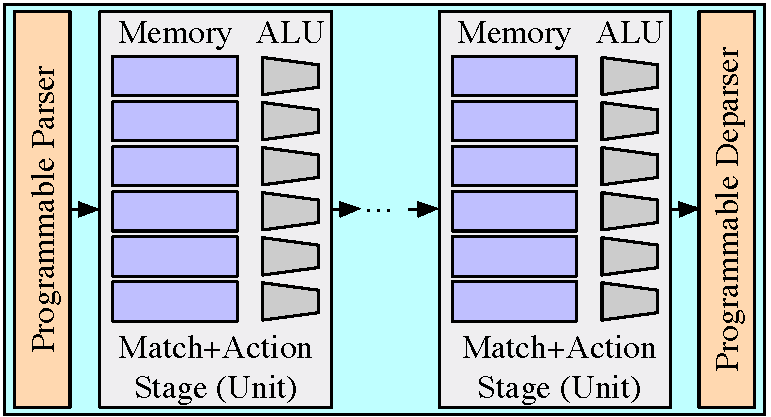
\includegraphics[width=0.54\columnwidth]{fig/mind/prog-pipeline.pdf}
  \vspace{-0.7em}
  \caption[Enabling technologies for \mind]{\textbf{Enabling technologies for \mind.} (left) Programmable switch architecture and (right) Switch ingress/egress pipeline.}
  \vspace{-0.5em}
  \label{fig:trad-directory}
  \label{fig:prog-pipeline}
  \label{fig:background}
\end{figure}

\begin{table}
  \caption[In-network technology tradeoffs]{\textbf{In-network technology tradeoffs.} See \S\ref{ssec:assumptions} for details.}\vspace{-1em}
  \label{fig:switchtradeoff}
  \scriptsize
    \renewcommand{\arraystretch}{1.2}
    \begin{tabular}{c|c|c|c|c}
      \hline
      & RMT & FPGA & Custom ASIC & CPU \\\hline\hline
      Line-rate & \cmark & \cmark & \cmark & \xmark \\
      Available & \cmark & \cmark & \xmark & \cmark \ \\
      Low Power & \cmark & \xmark & \cmark & \xmark\\
      Low Cost & \cmark & \xmark & \cmark & \xmark\\
      \hline
    \end{tabular}
  \end{table}

We now briefly describe \mind's enabling technologies.

\paragraphb{Programmable switches} In recent years, programmable switches have evolved along two well-coordinated directions: development of P4~\cite{p4, p4paper, dcp4}, a flexible programming language for network switches, and design of switch hardware that can be programmed with it~\cite{rmt, progswitch2, progswitch3, progswitch4}. These switches host an application-specific integrated circuit (ASIC), along with a general purpose CPU with DRAM, as shown in Figure~\ref{fig:background}~(left). The switch ASIC comprises ingress pipelines, a traffic manager and egress pipelines, which process packets in that order. Programmability via P4 is facilitated through a programmable parser and match-action units in the ingress/egress pipelines, as shown in Figure~\ref{fig:prog-pipeline}~(right). Specifically, the program defines how the parser parses packet headers to extract a set of fields, and multiple stages of match-action units (each with limited TCAM/SRAM and ALUs) process them. The general purpose CPU is connected to the switch ASIC via a PCIe interface, and serves two functions: (i) performing packet processing that cannot be performed in the ASIC due to resource constraints, and, (ii) hosting controller functions that compute network-wide policies and push them to the switch ASIC.

While the above focuses on switch ASICs with Reconfigurable Match Action Tables (RMTs)~\cite{rmt}, it is possible to realize \mind using FPGAs, custom ASICs, or even general purpose CPUs. While each of them exposes different tradeoffs (Table~\ref{fig:switchtradeoff}), we adopt RMT switches due to their performance, availability, power and cost efficiency.

\paragraphb{DSM Designs} Traditionally, shared memory has been explored in the context of NUMA~\cite{sgiorigin, amdopteron1, amdopteron2, intelqpi1, intelqpi2} and distributed shared memory (DSM) architectures~\cite{munin, midway, dpram, gam, dash}. In such designs, the virtual address space is partitioned across the various nodes, \ie, each partition has a \textit{home} node that manages its metadata, \eg, the page table. Each node also additionally has a cache to facilitate performance for frequently accessed memory blocks. We distinguish memory blocks from pages since caching granularities, \ie, block, can be different from memory access granularities, \ie, page. 

With the copies of blocks potentially residing across multiple node caches, coherence protocols~\cite{msi, mesi, mesif, moesi, mosi} are required to ensure each node operates on the latest version of a block. In popular directory-based invalidation protocols like MSI~\cite{msi} (used in \mind), each memory block can be in one of three states: \textbf{M}odified (\textbf{M}), where a single node has exclusive read and write access to (or, ``owns'') the block, \textbf{S}hared (\textbf{S}), where one or more caches have shared read-only access to the block, and \textbf{I}nvalid (\textbf{I}), where the block is not present in any cache. A directory tracks the state of each block, along with the list of nodes (``sharer list'') that currently hold the block in their cache. The directory is typically partitioned across the various nodes, with each home node tracking directory entries for its own address space partition. Memory access for a block that is not local involves contacting the home node for the block; it triggers a state transition and potential invalidation of the block across other nodes, followed by retrieving the block from the node that owns the block. While it is possible to realize more sophisticated coherence protocols, we restrict our focus to MSI in this work due to its simplicity --- we defer a discussion of other protocols to \S\ref{sec:discussion}.

As outlined in \S\ref{sec:intro}, extending the benefits of resource disaggregation to memory and making them widely applicable to cloud services demands (i) low-latency and high-throughput access to memory, (ii) a transparent memory abstraction that supports elastic scaling of memory \textit{and} compute resources without requiring modifications to existing applications. Unfortunately, prior designs for memory disaggregation expose a hard tradeoff between the two goals. Specifically, transparent elastic scaling of an application's compute resources necessitates a shared memory abstraction over the disaggregated memory pool, which imposes non-trivial performance overheads due to the cache-coherence required for both application data \textit{and} memory management metadata. We now discuss why this tradeoff is fundamental to existing designs. We focus on page-based memory disaggregation designs here, and defer the discussion of other related work to \S\ref{sec:related}.

\paragraphb{Transparent designs} While transparent DSMs have been studied for several decades, their adaptation to disaggregated memory has not been explored. We consider two possible adaptations for the approach outlined in \S\ref{ssec:assumptions} to understand their performance overheads, and shed light on why they have remained unexplored thus far. The first is a \textit{compute-centric} approach, where each compute blade owns a partition of the address space and manages the corresponding metadata, but the memory itself is disaggregated. A compute blade must now wait for several sequential remote requests to be completed for every un-cached memory read or write, \eg, to the remote home compute blade to trigger state transition for the block and invalidate relevant blades, and to fetch the memory block from the blade that currently owns the block. An alternate \textit{memory-centric} design that places metadata at corresponding home memory blades still suffers multiple sequential remote requests for a memory access as before, with the only difference being the home node accesses are now directed to memory blades. While these overheads can be reduced by caching the metadata at compute blades, it necessitates coherence for the metadata as well, incurring additional design complexity and performance overheads.

\paragraphb{Non-transparent designs} Due to the anticipated overheads of adapting DSM to memory disaggregation, existing proposals limit processes to a single compute blade~\cite{industry0, industry1, memdisagg1, infiniswap, legoos, disagg}, \ie, while compute blades cache data locally, different compute blades do not share memory to avoid sending coherence messages over the network. As such, these proposals achieve memory performance only by limiting transparent compute elasticity for an application to the resources available on a single compute blade, requiring application modifications if they wish to scale beyond a compute blade. 

\begin{table}
    \caption[Parallels between memory \& networking primitives]{\small \textbf{Parallels between memory \& networking primitives.}}\vspace{-1em}
    \label{table:isomorph}
    \centering
    \scriptsize
    %\setlength{\tabcolsep}{1pt}
    \renewcommand{\arraystretch}{1.2}
    \begin{tabular}{p{2cm} p{0.7cm}p{2cm}}
      \hline
      \textbf{Virtual Memory} &$\Longleftrightarrow$ &\textbf{Networking} \\\hline\hline
      Memory allocation&&IP assignment\\
      Address translation &&IP forwarding\\
      Memory protection  &&Access control\\
      Cache invalidations &&Multicast\\
      \hline
    \end{tabular}
    \vspace{-1em}
\end{table}

\section{\mind Overview}
\label{sec:mindoverview}

\begin{figure*}[!t]
\centering
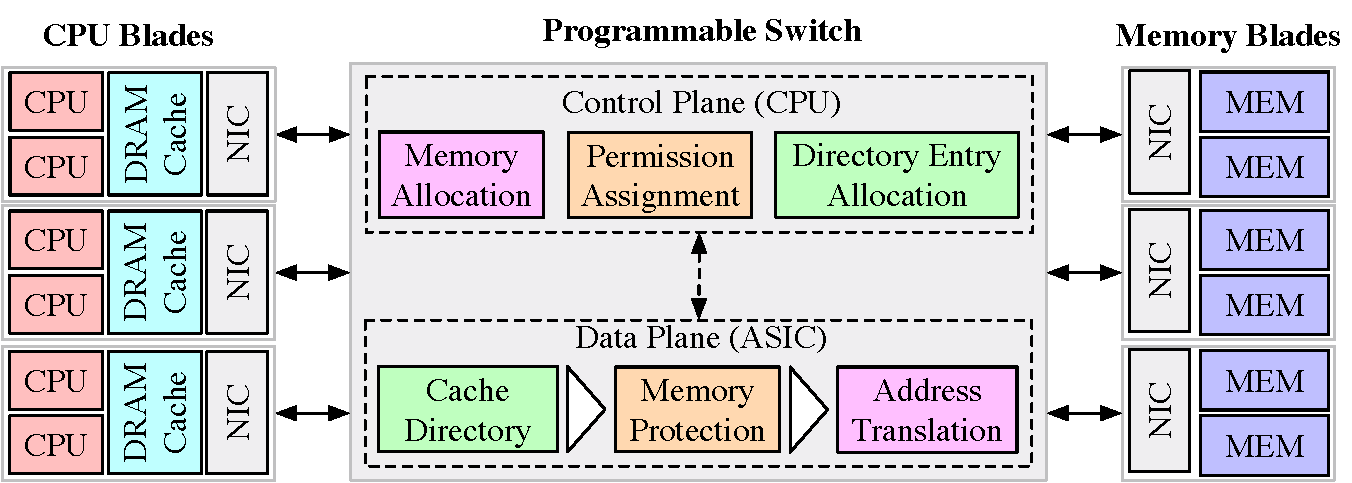
\includegraphics[width=0.55\textwidth]{fig/mind/design}\hspace{3em}
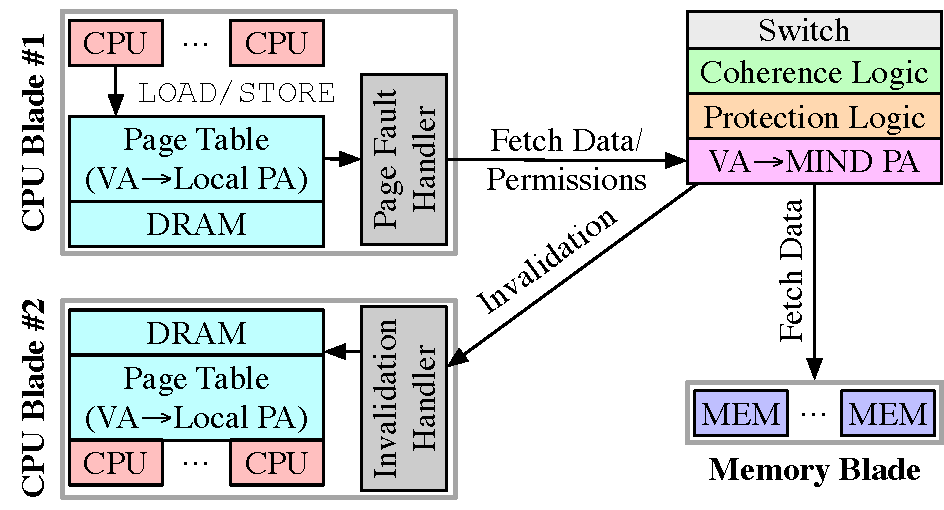
\includegraphics[width=0.35\textwidth]{fig/mind/data_flow}%\vspace{-1em}
\vspace{-0.5em}
\caption[High-level \mind architecture and data flow for memory accesses in \mind]{\textbf{(left) High-level \mind architecture, and, (right) data flow for memory accesses in \mind.} See \S\ref{ssec:design} for details.}
\label{fig:system_diagram}
\end{figure*}

To break the tradeoff highlighted above, we place memory management \textit{in the network fabric} for three reasons.
First, the network fabric enjoys a central location in the disaggregated architecture. Therefore, placing memory management in the data access path between compute and memory resources obviates the need for metadata coherence. 
Second, modern network switches~\cite{progswitch1, progswitch2, progswitch3} permit the implementation of such logic in integrated programmable ASICs. We show that these ASICs are capable of executing it at line rate even for multi-terabit traffic. In fact, many memory management functionalities have similar counterparts in networking (\autoref{table:isomorph}), allowing us to leverage decades of innovation in network hardware and protocol design for disaggregated memory management.
Finally, placing the cache coherence logic and directory in the network switch permits the design of specialized in-network coherence protocols with reduced network latency and bandwidth overheads, as we show in \S\ref{sec:design}. 

Effective in-network memory management requires: (\text{i}) \emph{efficient storage}, by  minimizing in-network metadata given the limited memory on the switch data plane;  (\textit{ii}) \emph{high memory throughput}, by load-balancing memory traffic across memory blades; (\textit{iii}) \emph{low access latency to shared memory}, via efficient cache coherence design that hides the network latency.

Next we elicit  three design principles followed by \mind to realize the above goals and provide an overview of its design.

\subsection{Design Principles}
\label{ssec:principles}

\mind follows three principles to meet the goals for memory disaggregation outlined in \S\ref{sec:intro}:

\paragraphb{P1} \textit{Decouple memory management} functionalities to ensure each can be optimized for their specific goals.

\paragraphb{P2} Leverage \textit{global view} of the disaggregated memory subsystem at a centralized control plane to compute optimal policies for each memory management functionality.

\paragraphb{P3} Exploit \textit{network-centric hardware primitives} at the programmable switch ASIC to efficiently realize policies computed using \textbf{P2}.

\vspace{0.075in}\noindent

\mind follows principle \textbf{P1} to decouple memory allocation from addressing (\S\ref{subsec:addr_trans}), address translation from memory protection (\S\ref{subsec:mem_prot}),  cache accesses and eviction from coherence protocol execution (\S\ref{subsec:cache_dir}),  and employs principles \textbf{P2} and \textbf{P3} to efficiently realize their goals. Note that traditional server-based OSes are unable to leverage these principles due to  their reliance on \textit{fixed-function} hardware modules such as the MMU and memory controller --- most common implementations of such modules couple many memory management functionalities (\eg, address translation and memory protection in page-table walkers) for a host of complexity, performance, and power reasons~\cite{vmbook, seesaw, rmmlite}.

\subsection{Design Overview}
\label{ssec:design}

\mind exposes a \textit{transparent virtual memory} abstraction to applications, similar to server-based OSes. Unlike prior disaggregated memory designs, \mind places all \mmm in the network, instead of CPU or memory blades~\cite{infiniswap, fastswap}, or a separate global controller~\cite{legoos}. 

Figure~\ref{fig:system_diagram}~(left) provides an overview of \mind design, while Figure~\ref{fig:system_diagram}~(right) depicts the data flow for memory accesses in \mind. The \textit{CPU blades} run user processes and threads, and possess a small amount of local DRAM that is used as a cache. All memory allocations (\eg, via \texttt{mmap} or \texttt{sbrk}) and deallocations (\eg, via \texttt{munmap}) from the user processes are intercepted at the CPU blade, and forwarded to the \textit{switch control plane}. The control plane possesses a global view of the system, which it leverages to perform memory allocations, permission assignments, \etc, using principle \textbf{P2}, and respond to the user process. All memory \code{LOAD}/\code{STORE} operations from the user processes are handled by the CPU blade cache (\S\ref{ssec:caching}). The cache is virtually addressed\footnote{Note that while it is hidden from applications, CPU blades maintain a local page-based virtual memory abstraction to translate \mind virtual addresses to physical addresses for cached pages in local DRAM (Figure~\ref{fig:system_diagram}~(right)).}, and stores permissions for cached pages to enforce memory protection. If a page is not locally cached, the CPU blade triggers a page-fault and fetches the page from \textit{memory blades} using RDMA requests, evicting other cached pages if necessary. Similarly, if the memory access requires an update to a cached block's coherence state (\eg, \code{STORE} on a Shared or \textbf{S} block), a page-fault is triggered to initiate cache coherence logic at the switch. Note that the page-fault based design requires \mind to perform page-level remote accesses, although future CPU architectures may enable more flexible access granularities (\S\ref{sec:discussion}).

Since the CPU blade does not store memory management metadata, the RDMA requests are for virtual addresses and do not contain endpoint information (\eg, IP address) for the memory blade that holds the page. Consequently, the \textit{switch data plane} intercepts these requests. It then performs necessary cache coherence logic, including lookups/updates to the cache directory and cache invalidations on other CPU blades (\S\ref{ssec:caching}, \S\ref{sec:algorithm}). In parallel, the data plane also ensures the requesting process has permissions to access the requested page (\S\ref{subsec:mem_prot}). If no CPU blade cache holds the page, the data plane translates the virtual addresses to physical addresses (\S\ref{subsec:addr_trans}), forwarding the request to the appropriate memory blade. These memory management functionalities are decoupled as separate modules following \textbf{P1}, and efficiently realized in the switch ASIC following \textbf{P3}.

In \mind's design, the memory blades simply store the actual memory pages, and serve RDMA requests for physical pages. Unlike prior works that employ RPC handlers and polling threads~\cite{legoos}, \mind leverages one-sided RDMA operations~\cite{farm} to obviate the need for any CPU cycles on the disaggregated memory blades. This is a step towards true hardware resource disaggregation, where memory blades need no longer be equipped with any general-purpose CPUs.

% !TEX root = ../paper.tex
\section{\mind Design}
\label{sec:minddesign}

Placing memory management logic and metadata in the network provides the opportunity for simultaneously achieving memory performance and resource elasticity. We now describe how \mind optimizes for the individual goals of memory allocation and addressing (\S\ref{subsec:addr_trans}), memory protection (\S\ref{subsec:mem_prot}), and cache coherence (\S\ref{ssec:caching}), while operating under the constraints of programmable switches. Finally, we detail how \mind handles failures (\S\ref{subsec:acking}). %We now describe how \mind achieves the same.

% !TEX root = ../paper.tex
\subsection{Memory Allocation \& Addressing}
\label{subsec:addr_trans}

Traditional virtual memory uses fixed sized pages as the basic units for both translation and protection; as a result, it cannot achieve the goal of storage efficiency without increasing memory fragmentation: small pages reduce memory fragmentation but require more translation entries, and vice versa.  Following \textbf{P1}, \mind overcomes this by \textit{decoupling} address translation and protection.  That is, \mind's translation is blade-based while protection is \code{vma} based (\S\ref{subsec:mem_prot}).

\paragraphb{Storage-efficient address translation} \mind eschews page-based protection but uses a \textit{single global virtual address-space} across all processes, allowing translation entries to be shared across them. Our approach builds on decades of research on virtual memory designs that also exploit a single address space~\cite{cheri, cap, gam, grappa, opal}, but adds techniques to minimize storage overheads for in-network address translation.
In particular, \mind \textit{range partitions} the virtual address space across different memory blades, such that the entire virtual-address space maps to a contiguous range of physical address space. This allows us to use a single translation entry for each memory blade: any virtual address that falls within its range can be directly routed to that memory blade, minimizing the storage required on switch data plane. In \mind, this mapping only changes when new memory blades join, old ones retire or if memory is moved between blades.

\paragraphb{Balanced memory allocation \& reduced fragmentation} \mind's control plane, leveraging its global view of allocations (\textbf{P2}), tracks the total amount of memory allocated on each memory blade and places a new allocation on the blade with the least allocation, to achieve near-optimal load-balancing. We validate this empirically in \S\ref{sec:evaluation}.

Moreover, since there is a one-to-one mapping between virtual and physical addresses within a particular memory blade, \mind minimizes external fragmentation at each memory blade by using traditional virtual memory allocation schemes that have evolved to facilitate the same, \eg, first-fit allocator in our implementation~\cite{firstfit}.
The result of memory allocation is a virtual memory area (\texttt{vma}), identified by the base virtual address and length of the area, \eg, 
  {{\small <\texttt{0x00007f84b862d33b}, \texttt{0x400}>}}
for a $1$KB area. 
As will be elaborated in \S\ref{subsec:mem_prot}, \code{vma} is the basic unit of protection in \mind.
This allows multiple processes to have non-overlapping \code{vma}s on the same blade, minimizing memory fragmentation.
 
\paragraphb{Isolation} We note that \mindx's global virtual address-space does not compromise on \textit{isolation} between processes. First, since the switch intercepts allocation requests across all compute blades, and possesses a global view of valid allocations at any time, it can easily ensure allocations are non-overlapping across different processes. Second, we show in \S\ref{subsec:mem_prot} that \mind's \code{vma}-based protection allows flexible access control between processes in a single global virtual address-space.

\paragraphb{Transparency via outlier entries} \mindx's one-to-one mapping between virtual and physical addresses does not preclude supporting unmodified applications with static virtual addresses embedded within their binaries, or OS optimizations such as page migration~\cite{pagemigrations}, \ie, moving pages from one memory blade to another. \mind maintains separate \textit{range-based} address translations~\cite{rangetranslations} for physical memory regions that correspond to static virtual addresses or migrated memory. These \textit{outlier} entries are stored succinctly in the switch TCAM, where the TCAM's longest-prefix matching (LPM) property ensures that only the most specific entry (\ie, one with the longest prefix) is considered when translating a virtual address, ensuring correctness.

\subsection{Memory Protection}
\label{subsec:mem_prot}

As \mind decouples translation and protection, it uses a separate table to store memory protection entries in the data plane. 
Consequently, an application can assign access permissions to a \code{vma} of any size.
The size of this protection table is proportional to the number of \code{vma}s. We find this number is reasonably small in our experiments and the protection table can easily fit in the switch ASIC even for a wide range of memory-intensive applications (\S\ref{sec:evaluation}). This is because the first-fit allocator and Linux's \code{glibc} allocation requests~\cite{glibc-alloc} do a good job of ensuring \code{vma}s are large and contiguous. 

\paragraphb{Fine-grained, flexible memory protection} Similar to prior work on capability-based systems~\cite{cheri, capabilityaddr}, \mind supports two key abstractions: \textit{protection domains} and \textit{permission classes}. Protection domains identify the entity that may (or may not) have permissions to access a particular memory region of arbitrary size, while the permission class identifies what the entity can do to the memory region. 
\mind's control plane exposes a set of APIs for memory allocation and permission changes that allows an application to specify a protection domain identifier (\code{PDID}) for an arbitrary virtual memory area (\code{vma}) and assign a permission class (\code{PC}) to the pair \code{<PDID}, \code{vma>}. 
The mapping \code{<PDID}, \code{vma>} $\rightarrow$ \code{PC} is stored as an entry in the protection table in the data plane. For existing applications, \mind simply takes the process identifier (\code{PID}) as the \code{PDID},  and uses Linux memory permissions (\eg, read-only, read-write, \etc) as permission classes. Note that \mind \textit{can} support richer memory protection semantics than traditional OSes, \eg, user programs that serve multiple client sessions, such as ssh servers or database services, can assign a separate protection domain per session to prevent one session from accessing data from other sessions~\cite{cheri}. 

Following principle \textbf{P3}, we leverage TCAM-based parallel range matches in the programmable switch ASIC --- typically used for IP subnet matches --- to efficiently support fine-grained matching for \code{<PDID}, \code{vma>} entries embedded in memory access requests and obtain corresponding the permission class (\code{PC}). If there is a mismatch between \code{PC} and the memory access type, or the \code{<PDID}, \code{vma>} entry does not exist, the request is rejected.

\paragraphb{Optimizing for TCAM storage} One limitation of TCAM is that each of its entries can only match power-of-two ranges. \mind overcomes this by splitting an arbitrary-sized virtual address range into multiple power-of-two-sized entries. Note that the number of entries required for a range of size $s$ is upper-bounded by $\lceil\log_2(s)\rceil$. In order to meet our goal of storage efficiency in the switch data plane, the control plane (1) only performs virtual address allocations that are aligned with the power-of-two sizes to ensure each region can be represented using a single TCAM entry, and (2) coalesces adjacent entries with if they belong to the same protection domain and have the same permission class. Interestingly, memory allocations requested by underlying libraries (\eg, \texttt{glibc}) are mostly in power-of-two sizes anyway, enabling storage-efficiency for TCAM entries.

\subsection{Caching \& Cache Coherence}
\label{ssec:caching}

In \mind design, while the caches\footnote{Note that we use the term `cache' to refer to the DRAM at the CPU blade under the partial disaggregation model, and not hardware (L1/L2/L3) caches.} reside on compute blades, the coherence directory and logic reside in the switch. This already permits access to the cache directory in half a round-trip, significantly reducing the latency overheads for the coherence protocol execution. For MSI protocol, even the most expensive and relatively uncommon transitions (\ie, \textbf{M}$\rightarrow$\textbf{S/M}) incur two round-trips, while common transitions incur only a single round-trip, as we show in \S\ref{ssec:bottlenecks}. While performance is a primary objective in \mind's cache coherence, the coherence protocol must also be realizable under the compute and memory constraints of switch ASICs. We now outline challenges in adapting traditional cache management to our in-network setting, along with how \mind resolves them.

\subsubsection{Storage vs. performance tradeoff}\label{ssec:storagevsperf}\hfill\\
Traditional caching and cache coherence mechanisms applied to \mind expose a tradeoff between cache performance and the storage efficiency at the switch data plane. Specifically, reducing the number of directory entries requires larger cache granularities (\ie, larger memory blocks), which results in worse performance. For instance, when large (\eg, $2$ MB) memory blocks are used, updating a small (\eg, $4$ KB) region within the block will invalidate the entire block. We refer to these invalidations as \emph{false invalidations} --- dirty pages invalidated along with the requested page because there are in the same memory block tracked by a directory entry. This leads to wastage in both memory bandwidth and cache capacity, \ie, fewer frequently accessed data items in the cache. We empirically highlight this tradeoff in \S\ref{ssec:sensitivity}.

\mind addresses this challenge using two approaches: it decouples the cache and directory granularities (following principle \textbf{P1}), and appropriately sizes the memory region tracked by each cache directory entry leveraging the global view of memory traffic at the control plane (following principle \textbf{P2}), as we describe next.

\paragraphb{Decoupling cache access \& directory entry granularities} Our first approach employs principle \textbf{P1} --- decoupling the granularity of cache (and memory) accesses from the granularity at which cache coherence is performed. This allows memory accesses (\eg, evictions or remote memory reads) to be performed at finer granularities, while directory entries are tracked at coarser granularities. Specifically, accesses to the local DRAM cache at CPU blades, and even the movement of data between the CPU caches and memory blades, occur at the fine page granularity ($4$ KB in \mind, similar to prior work~\cite{legoos, infiniswap, fastswap}). However, the coherence protocol tracks directory entries (stored at the switch data plane) at larger, variable-sized \textit{region} granularities --- when a $4$ KB page is cached at a CPU blade, \mind creates a directory entry for the region that contains the page. An invalidation of the region triggers an invalidation of all dirty pages in the region, as tracked by the individual CPU blades that cache them.

\paragraphb{Storage \& performance-efficient sizing of \textit{regions}} Even with the decoupling described above, the region \textit{sizes} still expose a tension between coherence performance (\eg, larger false invalidation counts due to larger region sizes) and directory storage efficiency (\eg, more directory entries due to smaller region sizes). To appropriately size regions, \mind leverages global view of memory traffic at the switch control plane (\textbf{P2}). Briefly, \mind starts each directory entry with a very large memory region; when the overhead due to false invalidation is high, it splits the region and creates a new directory entry. It does so repeatedly, until either the overhead is below a predetermined threshold, or the region size reaches $4$~KB, \ie, the page size. In doing so, \mind dynamically customizes the region sizes to resolve the tension between performance and directory storage efficiency using a novel \sizing algorithm --- we defer its details to \S\ref{sec:algorithm}.

\subsubsection{In-Network Coherence Protocol}\label{subsec:cache_dir}\hfill\\
\noindent
Due to the limited computational capability at the switch ASIC, \mind employs the simple directory-based MSI coherence protocol~\cite{msi}. While we defer the implementation details of the coherence protocol to \S\ref{ssec:switchimpl}, we highlight here how \mind employs network-centric hardware primitives to efficiently realize the coherence protocol in the switch, leveraging principle \textbf{P3}. Specifically, several state transitions in the MSI protocol require generating invalidation requests to CPU blades that have shared access to a region, to ensure correctness. To facilitate this in a network-efficient manner, we leverage \textit{multicast} functionality supported natively in most switches --- we create a multicast group for all CPU blades in the rack, and send an invalidation request containing the list of sharers to the group. However, broadcasting invalidations to blades not in the sharer list would consume unnecessary network bandwidth. As such, we embed the sharer list within the invalidation request, and drop requests in the egress path of the switch data plane if the output port does not lead to a blade in the sharer list.

\subsection{Handling Failures}\label{subsec:acking}

We now discuss how \mind handles failures at different components in our disaggregated architecture.

\paragraphb{CPU, memory blade and switch failures} \mind does not innovate on fault-tolerance for CPU and memory blade failures: mechanisms developed in prior work~\cite{legoos, infiniswap, disaggfault} for fault tolerance can be readily adapted to our design. To handle switch failures, we consistently replicate the control plane at a backup switch --- on a failure, the data plane state is reconstructed at the backup switch using the control plane state. Since the control plane is only updated infrequently due to metadata operations (\eg, system calls), the overhead added due to such replication in minimal.

\paragraphb{Communication failures} \mind uses ACKs and timeouts to detect packet losses. When a memory access triggers invalidations, the requesting compute blade waits for ACKs indicating successful invalidation from all sharers, and resends the request if timeout occurs. If the compute blade does not receive an ACK even after a predefined number of retransmissions, it sends a \code{reset} message for the corresponding virtual address to the switch control plane. This, in turn, forces all compute blades to flush their data for that address and removes the corresponding cache directory entry in the data plane. This \code{reset} mechanism prevents deadlocks when compute blades fail in the middle of a cache coherence state transition.


% !TEX root = ../paper.tex

\section{\mindAlgo: Algorithm \& Analysis}
\label{sec:algorithm}

We next provide details and a formal analysis of the \mindalgo algorithm used by \mind to dynamically determine the memory region size tracked by each cache directory entry.  This algorithm is a key component of \mind's cache coherence design outlined in \S\ref{ssec:caching}.

\subsection{Algorithm}
\label{ssec:detail}

The \mindalgo algorithm starts by partitioning the entire virtual address space into $N$ contiguous regions of size $M$ pages each. It then works in disjoint \emph{epochs} of equal length. In each epoch, it tracks the total number of times any page is falsely invalidated within the epoch  --- we refer to this as the \textit{false invalidation count} --- for every region.

\mindAlgo uses false invalidation count as a measure of the performance overhead --- we characterize the impact of false invalidations on performance in \S\ref{sec:evaluation}. It therefore seeks to keep the count below a threshold, denoted by $t$. 
If any region has a false invalidation count $> t$ in an epoch, it splits that region into two equal halves and creates a new directory entry accordingly. It bounds the smallest size of any memory region to $4$KB (the page size), ensuring that any $M$ sized block is split at most $\log_2{M}$ times over as many epochs. Note that for 4KB regions, the number of falsely invalidated pages is trivially zero; however, maintaining all regions at that size would require storing $N\cdot M$ directory entries at the switch, which is impractically large. 


\paragraphb{Stability assumptions} The \mindalgo is based on two implicit assumptions related to the epoch length:
\begin{itemize}[itemsep=0pt, leftmargin=*]
  \item the access pattern across the various memory regions remains stable for at least $O(\log_2{M})$ epochs, and
  \item the set of allocated pages remains unchanged across $O(\log_2{M})$ epochs.
\end{itemize}

\noindent
We show in \S\ref{sec:evaluation} that appropriate epoch sizing allows us to ensure both assumptions for our evaluated workloads.

\subsection{Performance Bounds}
\label{ssec:bound}
The key challenge in \mindalgo is bounding the number of directory entries that must be stored, one per memory region. The total \textit{worst-case} number of regions depends on two factors: (i) worst-case number of \textit{sub}-regions generated by each $M$-sized region, and (ii) the value of $t$. We first analyze the worst-case bound on the number of sub-regions per $M$-sized region, and then bound the worst-case for total number of regions overall (and therefore, the total number of directory entries) by appropriately setting the value of $t$.


\paragraphb{Bounding the number of sub-regions per $M$-sized region} We establish the worst-case bound in the following theorem:

\begin{myTheorem}\label{theorem:region}
  The number of sub-regions for an $M$-sized region with false invalidation count $f$ is upper-bounded by $S=(\lceil\frac{f}{t}\rceil-1)\cdot(1+\log_2{M})$.
\end{myTheorem}
\begin{proof}
  In the \mindalgo algorithm, we dynamically manage sizes of each memory region, splitting it into two smaller regions until the false invalidation count for the region is less than $t$. As noted above, since we limit the smallest region size to 4KB, an $M$-sized region may be split at most $\log_2{M}$ times, across as many epochs. Figure~\ref{fig:cache_tree} depicts the splitting process as a binary tree across the various epochs, where the level of the tree $l$ denotes the epoch index ($0 \leq l < \log_2{M}$). For the sake of exposition, we set $M=2$MB. We leverage two observations to prove the above bound:
  \begin{itemize}[itemsep=0pt, leftmargin=*]
    \item{\textbf{O1:}} Splitting a region can only \textit{decrease} the false invalidation count across the two splits, \ie, if a region with $f$ false invalidation count is split into two regions with $f'$ and $f''$ false invalidation count, then $f' + f'' \leq f$.
    \item{\textbf{O2:}} For a 4KB region, the false invalidation count is zero.
  \end{itemize}  
  
\begin{figure}[t]
  \centering
  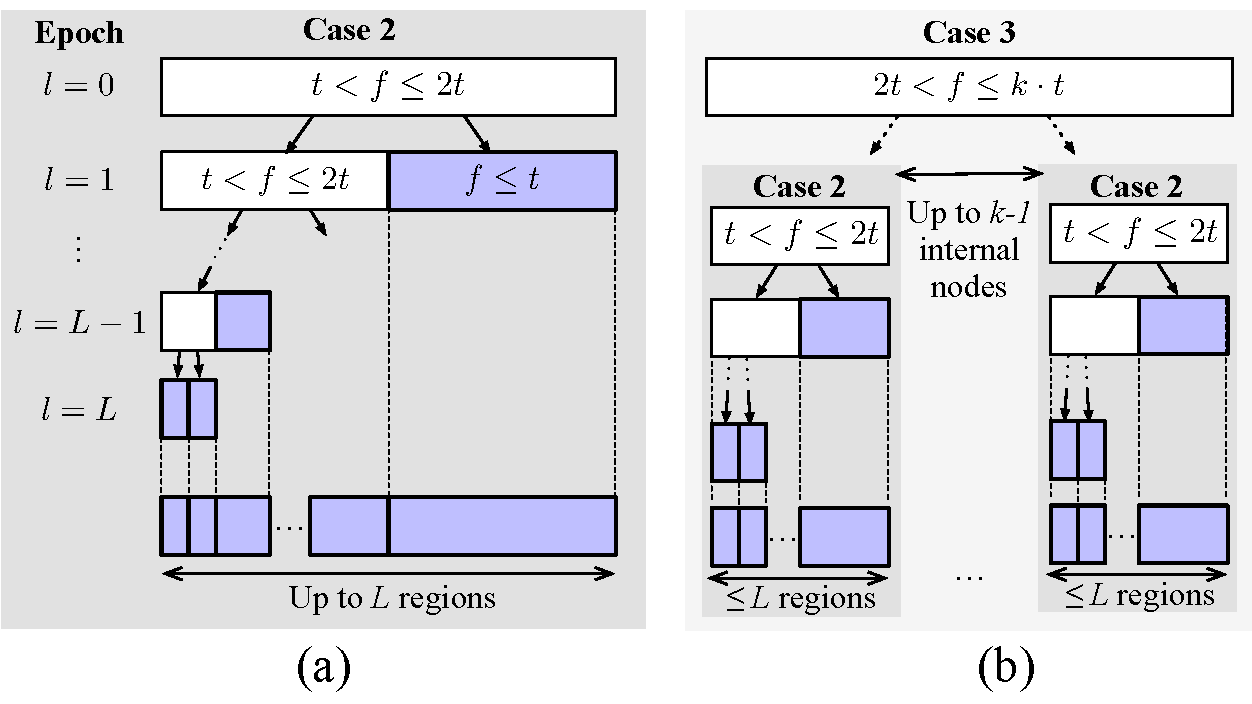
\includegraphics[width=0.97\columnwidth]{fig/mind/proof_fig.pdf}\vspace{-1em}
  \caption[Splitting process for cache blocks depicted as a binary tree]{\textbf{Splitting process for cache blocks depicted as a binary tree.} Note that $L=\log_2{M}$; see 
  \S\ref{ssec:bound} for details.}\label{fig:cache_tree}
  \vspace{-0.5em}
\end{figure}
  
  \noindent
  The maximum number of regions $S$ generated by splitting an $M$-sized region can be categorized into three cases:
  
  \paragraphb{Case 1: $f \leq t$} Since false invalidation count is already below the threshold, the region does not need to be split, \ie, $S=1$.
  
  \paragraphb{Case 2: $t < f \leq 2t$} To bring the false invalidation count below $t$, the region will be split into two. Due to observation \textbf{O1}, there are two possibilities: (i) both resulting regions have false invalidation count $<t$, or (ii) one region $r_1$ still has false invalidation count $>t$ while the other region $r_2$ has false invalidation count $<t$. For (i), the resulting regions do not need to be split any further, while for (ii), $r_1$ must be split further in the next epoch. In the worst case, the splits will continue for at most $\log_2{M}$ epochs --- when the region size reaches 4KB, no further splits will be required (due to observation \textbf{O2}). Thus, $S = 1 + \log_2{M}$, as shown in Figure~\ref{fig:cache_tree}~(a).
  
  \paragraphb{Case 3: $2t < f \leq k\cdot t$, where $k = \lceil\frac{f}{t}\rceil$} The worst-case scenario that maximizes the number of generated regions must maximize the number of ``internal nodes'' that can generate such regions in the binary tree depicting the splitting process. In particular, the scenario should create as many internal node regions with false invalidation count between $t$ and $2t$ as possible, and then employ \textbf{Case 2} to maximize the number of final regions generated by each ``internal node'' region. Note that for $2t < f < k\cdot t$, the region may be split into at most $k - 1$ regions where each region has false invalidation count between $t$ and $2t$ (regardless of how many epochs it takes). With the worst-case number of regions generated by each such internal node region given in \textbf{Case 2}, the upper bound on the number of generated regions is given by (Figure~\ref{fig:cache_tree}~(b)):
  $$S = (k - 1) \cdot (1 + \log_2{M}) = (\lceil\frac{f_i}{t}\rceil - 1) \cdot (1+\log_2{M})$$
  \noindent
  As such, across the three cases, the total number of regions is at most $(\lceil\frac{f}{t}\rceil - 1) \cdot (1+\log_2{M})$.
\end{proof}

\paragraphb{Bounding the total number of regions} We now consider the worst-case number of regions $S_{max}$ contributed by \textit{all} $M$-sized regions. Let $f_i$ be the number of false invalidation count for an $M$-sized region $i$ ($1 \leq i \leq N$), and $S_i$ be the worst-case number of regions generated by it, then:
$$ S_{max} = \sum\limits_{i=1}^{N} S_i = \sum\limits_{i=1}^{N} (\lceil\frac{f_i}{t}\rceil - 1) \cdot (1+\log_2{M}) $$
\noindent
To bound $S_{max}$, we must set $t$ appropriately. In order to ensure fairness across all $M$-sized regions, we set the threshold $t$ as a fraction of the average false invalidation across them, \ie, 
\begin{align}\label{eq:t}
  t = \frac{1}{c\cdot N} \cdot \sum\limits_{i=1}^{N} f_i
\end{align}
\noindent
where $c$ is a constant parameter.

This allows us to bound $S_{max}$ as follows:
\begin{align*}
  S_{max} &= \sum\limits_{i=1}^{N} (\lceil\frac{f_i}{t}\rceil - 1) \cdot (1+\log_2{M}) \leq \sum\limits_{i=1}^{N} \frac{f_i}{t} \cdot (1+\log_2{M})                &\\
          &= c \cdot N \cdot (1+\log_2{M}) \text{$\qquad$(From Eq.~\ref{eq:t})}
\end{align*}
\noindent
If use up all the available switch data plane capacity to store $S_{max}$ entries, we can set $c$ as $\frac{S_{max}}{N\cdot(1+\log_2{M})}$, which will always ensure the total number of regions is $\leq S_{max}$.

\paragraphb{Split vs. merge-based approach} The approach we have described so far starts with $M$-sized regions, and splits into regions until the false invalidation count for each region reduces below the threshold $t$. An alternate but equivalent strategy would begin with 4KB regions and merge them into larger regions as long as the false invalidation count per region remains below $t$. In fact, it is possible to begin with any intermediate region size, and split or merge as necessary. In \mind, we use a default of $16$KB since it provides a favorable tradeoff between storage and performance overheads for our evaluated workloads --- we defer a detailed analysis to \S\ref{sec:evaluation}.

\paragraphb{From theory to practice} At $c=1$, the dynamic resizing approach outlined above reduces the amount of storage required for directory entries from $M\cdot N$ to a worst-case of $(1+\log_2{M})\cdot N$ --- an \textit{exponential} decrease. At the same time, it ensures that the number of false invalidation count remains under $\frac{\sum f_i}{N}$. However, we note that our theoretical analysis only reveals the \textit{worst-case} --- in practice, we find both storage and performance overheads are much lower, as we show in \S\ref{sec:evaluation}. As such, we can set the value $c > 1$ to increase switch data plane storage utilization without hitting its capacity in practice. In fact, we dynamically adjust the value of $c$ such that the utilization of the switch data plane storage in any epoch remains below $95\%$.

% !TEX root = ../paper.tex
\section{\mind Implementation}
\label{sec:mindimpl}

We now describe \mind implementation. \mind exposes Linux memory and process management system call APIs, and splits its kernel components across CPU blade and the programmable switch. We now describe these kernel components, along with the RDMA logic required at the memory blade.

\subsection{CPU Blade}
\label{ssec:cpumemimpl}

\mind assumes a partial disaggregation model, where the CPU blades possess a small amount of local DRAM as cache (\S\ref{ssec:assumptions}). The CPU blades in our prototype use traditional servers with no hardware modifications. We implemented CPU blade kernel components as a modified Linux kernel 4.15. \mind provides transparent access to the disaggregated memory, by modifying how \code{vma}s and processes are managed and how page faults are handled at the CPU blade, as we detail next.

\paragraphb{Managing \code{vma}s} To handle the creation and removal of \code{vma}s due to process heap allocation/deallocation requests, such as \code{brk}, \code{mmap}, and \code{munmap}, the kernel module intercepts such requests from the process and forwards them to the control plane at the switch over a reliable TCP connection. The switch subsequently creates new \texttt{vma} entries, and responds with the same return value (\eg, virtual address of the allocated \code{vma}) as the local version of the system calls --- ensuring transparency for user applications. The switch returns Linux-compatible error codes (\eg, \code{ENOMEM}) if there are any errors.

\paragraphb{Managing processes} The kernel module also intercepts and forwards process creation and termination requests, such as \code{exec} and \code{exit}, to the switch control plane, which maintains the internal representation of processes (\ie, Linux's \code{task\_struct}) and a mapping between the compute blades and processes they host. \mind assigns threads running on different CPU blades the same PID if they belong to the same process, permitting them to transparently share the same address-space via memory protection and address translation rules installed at the switch. Finally, we do not focus on scheduling in this work and simply place threads and processes across compute blades in a round-robin manner.

\paragraphb{Page fault-driven access to remote memory} When a user application tries to access a memory address not present in the CPU blade cache, a page fault handler is triggered and the CPU blade kernel sends a one-sided RDMA read request to the switch with the virtual address and the requested permission class, i.e., read or write for Linux. At the same time, the page to be used by the user application is registered to the NIC as the receiving buffer, obviating the need for additional data copies. Once the page is received, the local memory structures such as PTEs are populated and the control is returned to the user. Our implementation of the CPU blade DRAM cache is similar to LegoOS~\cite{legoos}, but additionally handles cache invalidations for coherence. Specifically, the cache tracks the set of writable pages locally, and on receiving an invalidation request for a region, it flushes all writable pages in the region and removes all local PTEs.

While the above approach enables transparency for access to disaggregated memory, it presents a significant limitation in our implementation --- it restricts the memory consistency model in \mind to stronger Total Store Order (TSO), and precludes weaker consistency models, \eg, Process Store Order (PSO) used in DSM approaches~\cite{gam}. This is because unlike TSO, PSO enables multiple writes to a cached memory region to be propagated asynchronously, but blocks if there is a subsequent read to the same region. Realizing this relaxation using page faults requires such writes to be buffered at the compute blade's local DRAM cache without triggering a page fault, but triggering one on a subsequent read to the same page. Unfortunately, this is impossible in traditional x86 or ARM architectures, since they do not support triggering a trap on read without also triggering one for a write. Consequently, \mind's stricter TSO model results in limited scalability for workloads with high read/write contention to shared memory regions, as we show in \S\ref{subsec:macro_bench}. We discuss possible architectural changes to address this in \S\ref{sec:discussion}.

\subsection{Memory blade} 

Unlike prior disaggregated memory systems~\cite{legoos, infiniswap} or distributed shared memory systems~\cite{gam}, \mind does not require any compute logic or data plane processing logic to run on the memory blades, obviating the need for general purpose CPUs on them. However, since the memory blade in our prototype is realized on traditional Linux servers, we rely on the kernel module at the memory blade to perform RDMA-specific initializations. When a memory blade comes online, its kernel module registers physical memory addresses to the RDMA NIC and reports the mapped address to the global controller. However, subsequent one-sided RDMA requests from CPU blades are handled completely by the memory blade NIC without involving the CPUs. Ideally, memory blades would be realized with all logic, including initialization, completely in hardware, without a CPU. While this would facilitate a memory blade design that is both simple and cheap, it would require new hardware design.

\subsection{Programmable Switch}
\label{ssec:switchimpl}

The \mind programmable switch module is implemented on a 32-port EdgeCore Wedge switch with a $6.4$~Tbps Tofino ASIC and an Intel Broadwell processor, $8$~GB RAM and $128$~GB SSD. The general purpose CPU hosts the \mind control program, which performs process, memory and cache directory management. Meanwhile, the ASIC performs address translation (\S\ref{subsec:addr_trans}) and memory protection (\S\ref{subsec:mem_prot}), handles directory state transitions and virtualizes RDMA connections between compute and memory blades. We here provide implementation details of the mechanisms not already described in \S\ref{sec:design}.

\paragraphb{Process \& memory management} The control plane hosts a TCP server to handle system call intercepts from CPU blades, and maintains traditional Linux data structures for process/thread management (\code{task\_struct}) as well as memory management (\code{mm\_struct}, \code{vm\_area\_struct}). On receiving a system call, the control plane modifies the data structures accordingly, and responds with return values consistent with the system calls to ensure transparency.

\paragraphb{Cache directory management} \mind reserves a fixed amount of SRAM at the data plane for storing directory entries, and partitions it into fixed sized slots, one for each \textit{region} entry in \mind. The control plane maintains a \textit{free list} for available slots, and a hash table \textit{used map} which maps the base virtual address for the dynamically sized cache region to the SRAM slot storing its directory entry. All slots are initially added to the free list. \mind creates a directory entry for a region during its allocation by removing an SRAM slot from the free list, populating it with the directory entry with invalid (\textbf{I}) state, creating a match-action rule that maps the block virtual address to the SRAM slot at the data plane, and updating its \textit{used map}. A similar process occurs when a region is split, while removing a directory entry follows the reverse procedure.

\begin{figure}[t]
  \centering
  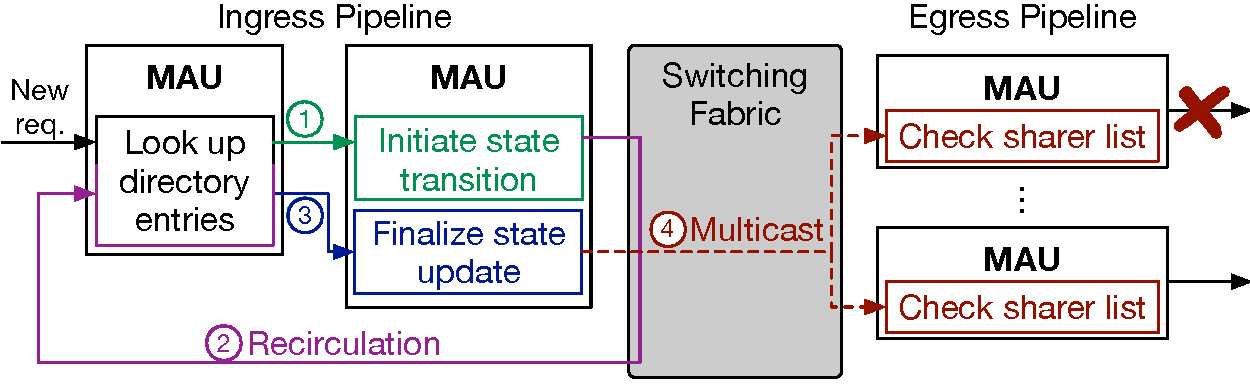
\includegraphics[width=0.97\columnwidth]{fig/mind/cc.pdf}
  \vspace{-0.7em}
  \caption[Performing directory state transitions on switch ASIC]{\textbf{Performing directory state transitions on switch ASIC.}}
  \vspace{-0.5em}
  \label{fig:cc_example}
\end{figure}

\paragraphb{Directory state transitions} We found that a single match-action unit (MAU) in today's switch ASICs is unable to (i) perform a directory entry lookup, (ii) determine the correct translation based on the current block state and memory access request, and (iii) update the directory entry accordingly all at once, due to their limited compute capability. As such, we split the logic for (i-ii) across two MAUs (\circled{1} in Figure~\ref{fig:cc_example}): the first MAU stores the directory entries and performs (i), while the second MAU stores a \textit{materialized} state-transition table containing all possible transitions and corresponding actions to be performed for (ii). Note that explicitly storing the state-transition table trades-off data plane memory capacity to overcome the limited compute cycles in an MAU. To perform (iii), the second MAU \textit{recirculates} the memory access request packet within the switch data plane to send it back to the first MAU (\circled{2}), so that it can update the directory entry according to actions determined by the second MAU (\circled{3}). If the state transition requires cache invalidations, the data plane creates invalidation requests leveraging \textit{multicast}, as described in \S\ref{subsec:cache_dir}. Specifically, these requests are only forwarded to the current sharers for the relevant page (\circled{4}).

\paragraphb{Virtualizing RDMA connections} When a compute blade in \mind issues an RDMA request, it does not know the location of the blade where the page resides. Consequently, the switch data plane in \mind \textit{virtualizes} RDMA connections between all possible CPU-memory blade pairs by transparently transforming and redirecting corresponding RDMA requests and responses between them. Specifically, once an RDMA request's destination blade is identified via address translation or cache coherence, the data plane updates the request's packet header fields such as IP/MAC addresses and RDMA-specific parameters, before forwarding it to the blade.

% !TEX root = ../paper.tex
%
\section{Evaluation}
\label{sec:mindevaluation}

\begin{figure*}[ht!]
  \centering
  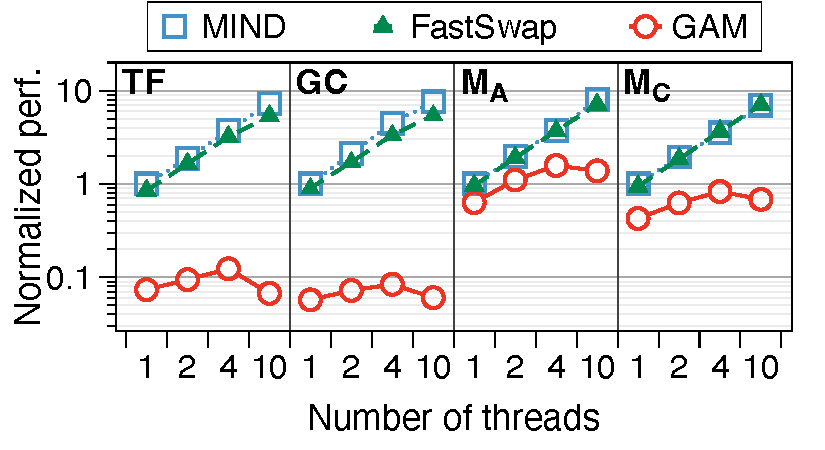
\includegraphics[width=0.345\textwidth]{fig/mind/04_intra}\hspace{-0.25em}
  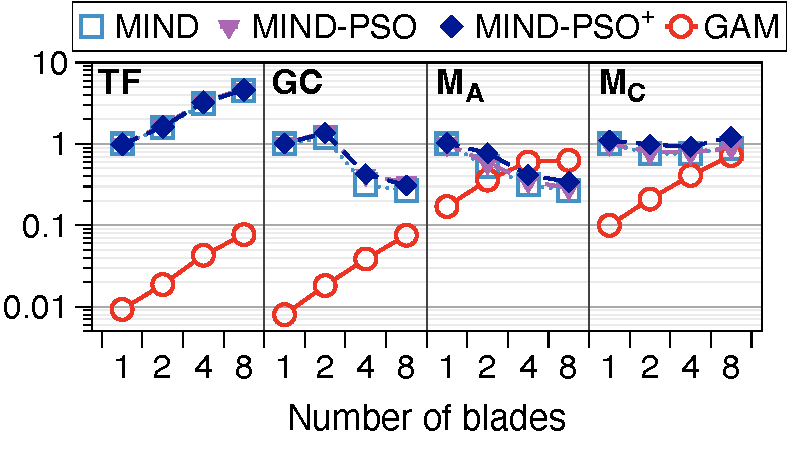
\includegraphics[width=0.3266\textwidth]{fig/mind/04_inter}\hspace{-0.25em}
  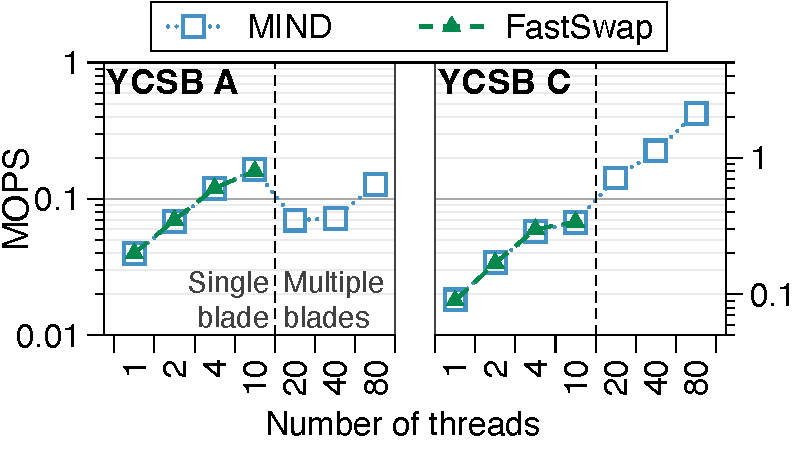
\includegraphics[width=0.3247\textwidth]{fig/mind/04_kvs}
  \vspace{-0.7em}
  \caption[Performance scaling]{\textbf{Performance scaling} (left) on a single compute blade, (center) across compute blades, and (right) for Native-KVS. For (center), each blade runs 10 threads. Performance is normalized by \mind's performance at 1 thread for (left) and 1 blade for (center); the runtimes in seconds for TF, GC, M$_A$ and M$_C$ workloads are 62.8, 59.3, 301.4 and 268.2 for 1 thread, and 69.2, 62.8, 302.3 and 306.9 for 1 blade, respectively.}
\label{fig:perf}
\label{fig:perf_intra}
\label{fig:perf_inter}
\label{fig:perf_kvs}
\end{figure*}


We evaluate \mind to answer the following questions:
\begin{itemize}[topsep=2pt, partopsep=0pt, itemsep=0pt, leftmargin=*]
  \item Can \mind enable transparent elasticity over performant disaggregated memory for real-world workloads (\S\ref{subsec:macro_bench})?
  \item What are \mind's performance/resource bottlenecks (\S\ref{ssec:bottlenecks})?
  \item How does \mindalgo perform in isolation (\S\ref{ssec:sensitivity})?
\end{itemize}
\paragraphb{Compared systems} We compare \mind against two extreme designs in disaggregated memory (\S\ref{ssec:challenges}): a \textit{transparent} DSM-based approach with cache-coherence that supports compute elasticity, and a \textit{non-transparent} approach that limits compute elasticity to a single compute blade. For the former, we adapt GAM~\cite{gam}, a software-based DSM, to our disaggregated setting where cache directory is implemented at the compute blades. For the latter, we employ FastSwap~\cite{fastswap}, a state-of-the-art swap-based disaggregated memory system. All systems employ RDMA for efficient remote memory accesses. Finally, \mind uses an initial region size of $16$~kB and epoch size of $100$~ms for its \mindalgo algorithm.

\paragraphb{Cluster setup} We used a cluster comprising five servers connected via the programmable switch described in \S\ref{ssec:switchimpl}. We used a single server equipped with two 18-core Intel Xeon processors, $384$~GB of memory and four Nvidia/Mellanox CX-5 $100$~Gbps NICs, to host multiple memory blade VMs. To highlight the overhead and scalability of in-network cache coherence protocol, we used the remaining four machines, each equipped two 12-core Intel Xeon processors and two Nvidia/Mellanox CX-5 $100$~Gbps NICs, to host two CPU blade VMs on each server. Similar to prior work~\cite{legoos}, we emulate the partial disaggregation model by limiting the local DRAM usage at each compute blade to $512$~MB, which is about $25\%$ of the memory footprint for our evaluated workloads. Note that each CPU and memory blade VM in our setup had dedicated access to a separate $100$~Gbps NIC to ensure they represent separate network attached entities.

\paragraphb{Applications and workloads} We use several real-world workloads in our evaluation: TensorFlow~\cite{tensorflow} with ResNet-50~\cite{resnet} on CIFAR-10~\cite{cifar10} (denoted as TF), GraphChi~\cite{graphchi} with PageRank~\cite{pagerank} on Twitter graph~\cite{twitter_graph} (denoted as GC), and Memcached~\cite{memcached} with YCSB~\cite{ycsb_workload} workload A ($50\%$ read, $50\%$ write split, denoted as M$_A$) and workload C ($100\%$ reads, denoted as M$_C$). Since GAM is a \textit{software} DSM system, it requires applications to use a specialized memory API, while \mind and FastSwap are transparent to applications. To ensure consistent comparison under different interfaces, we captured the memory accesses from our workloads using Intel's PIN~\cite{intel_pin}, and used a memory access emulator to generate the exactly same memory accesses across all three systems. In addition, we also present results for native execution of a simple key-value store (denoted as Native-KVS) on \mind and FastSwap, since they support a transparent memory interface.

\subsection{Performance Scaling for Real-World Workloads}\label{subsec:macro_bench}

We start by evaluating \mind's performance scalability.

\paragraphb{Intra-blade scaling} Figure~\ref{fig:perf_intra}~(left) shows performance scaling across all systems as the number of threads is increased on a single compute blade. We report performance as the inverse of runtime, normalized by the performance of \mind for 1 thread. \mind and FastSwap scale almost linearly with more compute blades because of their efficient page-fault driven remote memory accesses. In contrast, GAM scales linearly only up to 4 threads, and sub-linearly after that due to software overheads from its user-level library. For instance, GAM must check access permissions for every memory access by acquiring a lock, while \mind and FastSwap can leverage the hardware MMU to facilitate the same. Such overheads become significant as the compute resources on a single compute blade come under contention at $10$ threads running on a $12$-core node. 

\paragraphb{Inter-blade scaling} Next, we evaluate inter-blade scalability by running $10$ execution threads per-blade, for up to $8$ compute blades. Figure~\ref{fig:perf_inter}~(center) shows our results; here, while \mind's default memory consistency model is strict (TSO, \S\ref{sec:impl}), \mind-PSO denotes the \textit{simulated} performance of \mind with the weaker PSO model (same as GAM). \mind-PSO$+$ additionally simulates the effect of infinite switch capacity for directory storage. Since we are forced to simulate \mind-PSO and \mind-PSO$+$ using traces collected on a real TSO-based system, the traces retain additional TSO-associated queuing delays that we cannot elide, \ie, while our simulations can reorder writes and non-conflicting reads, queuing delays remain; in other words, our \mind-PSO and \mind-PSO$+$ results are underestimates to potential performance of a hardware-based solution. Finally, we omit FastSwap as it does not transparently scale beyond a single compute blade, similar to other disaggregation proposals~\cite{legoos, infiniswap}.

For a machine learning workload (TF), \mind's performance scales well despite its stricter memory consistency model compared to GAM --- doubling the number of compute blades improves \mind's performance by ${\sim} 1.67\times$, with a $59 \times$ speeded compared to GAM at $8$ compute blades. For GC, \mind's performance increases from $1$ to $2$ compute blades, but starts to decrease beyond that. This is because GC's graph traversals incur random and often contentious access to shared data compared to machine learning workloads in TF. GC writes ${\sim} 2.5\times$ more data in shared pages than TF, generating significantly more state transitions to modified (\textbf{M}) state, and incurring frequent invalidations (\S\ref{ssec:bottlenecks}). PSO partly alleviates this overhead by permitting writes to be performed asynchronously, but still does not permit linear scaling beyond $2$ compute blades. Instead, GAM scales better because the performance differential between its local and remote accesses is small --- local accesses are $10\times$ slower than that of MIND (due to software implementation of local accesses), while remote access latencies are similar for both. Consequently, performing more remote accesses (during invalidations) does not impact GAM performance as much as it does for \mind.

Finally, M$_A$ and M$_C$ have more sharers with much larger number of shared writes compared to TF and GC. As a result, \mind does not scale well beyond $1$ compute blade because: (1) more blades contend for acquiring write permission to the same region incurring multiple invalidations and significantly smaller number of local memory accesses, and (2) the directory storage at the switch becomes a bottleneck (as we show in \S\ref{ssec:bottlenecks}), frequently resulting in false invalidations for heavily shared memory regions. We confirm these insights through \mind-PSO and \mind-PSO$+$ simulated results, which show that employing weaker memory consistency models and infinite directory capacity improves \mind's performance to some extent. Note that for M$_C$, \mind's performance increases from $4$ to $8$ blades since the number of invalidations do not increase by much. GAM scales better due to its weaker consistency model, and by leveraging its software implementation to facilitate several memory access reorderings which are not possible in \mind. Consequently, at $8$ compute blades, GAM and \mind-PSO$+$ achieve roughly similar performance.

\paragraphb{Native KVS} Figure~\ref{fig:perf_kvs}~(right) shows the intra- and inter-blade scaling of Native-KVS on \mind and FastSwap for YCSB-A and C workloads. On a single blade, both \mind and FastSwap observe near linear performance scaling for up to $10$ threads. Since FastSwap does not support sharing state across multiple compute blades, we do not report its performance beyond $10$ threads. Similar to our results for M$_A$, \mind does not scale well beyond a single compute blade for the YCSB-A workload ($50\%$ reads, $50\%$ writes) due to high read-write contentions. For the YCSB-C workload, Native-KVS scales linearly even beyond a single blade since it is a read-only workload, incurring no invalidations. Interestingly, YCSB-A workload on Native-KVS scales better than M$_A$ --- we attribute this to better partitioning of KVS state across compute blades in Native-KVS compared to Memcached.

\subsection{\mind's Performance and Resource Bottlenecks}
\label{ssec:bottlenecks}

We study \mind bottlenecks in terms of (i) memory access performance, and (ii) memory resources at the switch.

\begin{figure}[t!]
  \centering
  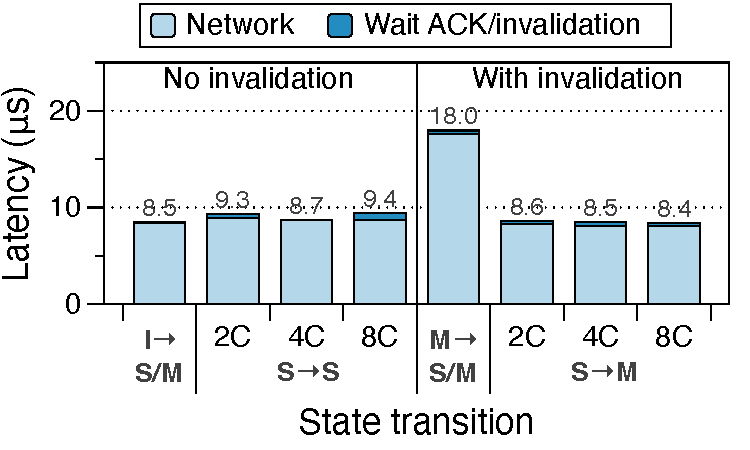
\includegraphics[width=0.58\linewidth]{fig/mind/15_transition_latency}\hfill
  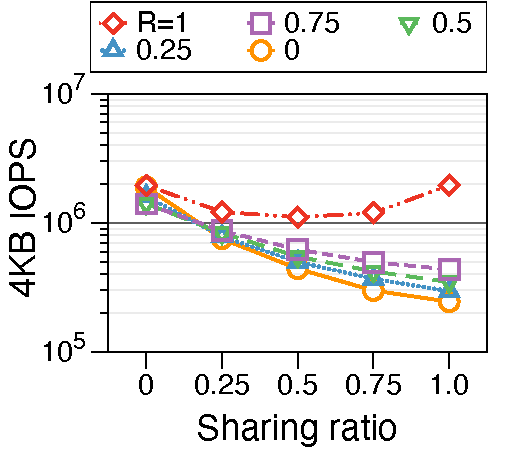
\includegraphics[width=0.40\linewidth]{fig/mind/16_sharing_ratio}
  \vspace{-0.9em}
  \caption[Performance bottlenecks]{\textbf{Performance bottlenecks.} (left) Network latency for state transitions, (right) memory throughput vs. read-write/sharing ratios.}
  \label{fig:micro_latency}
  \label{fig:micro_band} 
  \label{fig:perfbottlenecks}
\end{figure}

\begin{figure*}[ht!]
  \centering
  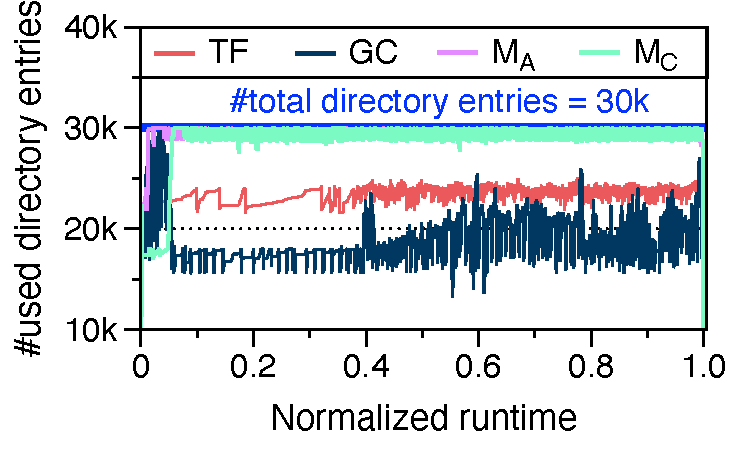
\includegraphics[width=0.3\textwidth]{fig/mind/09_switch_entries_over_time}\hspace{1em}
  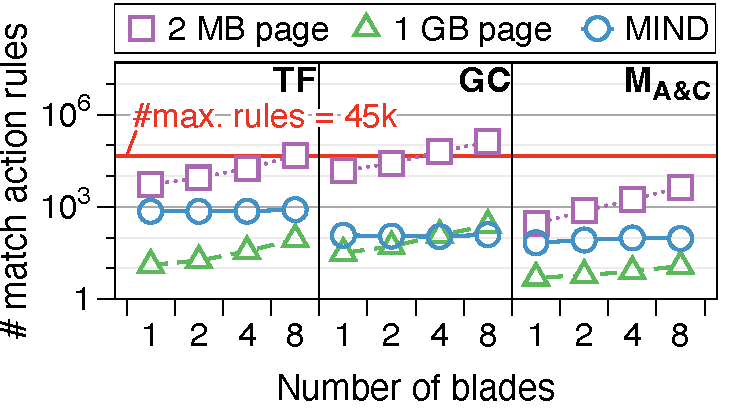
\includegraphics[width=0.31\textwidth]{fig/mind/12_micro_num_entry}\hspace{1em}
  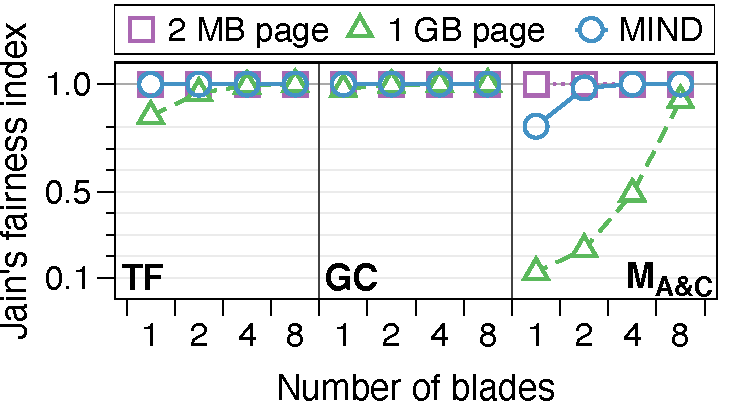
\includegraphics[width=0.31\textwidth]{fig/mind/12_micro_load_balance}
  \vspace{-0.9em}
  \caption[\mind switch resource bottlenecks]{\textbf{\mind switch resource bottlenecks.} (left) Directory entries, (center) match-action entries for heap, (right) load balancing for heap.}
  \label{fig:resbottlenecks}
  \label{fig:micro_load_balance}
  \label{fig:micro_num_entry}
  \label{fig:macro_cache_dir}
\end{figure*}

\begin{figure*}[t!]
  \centering
  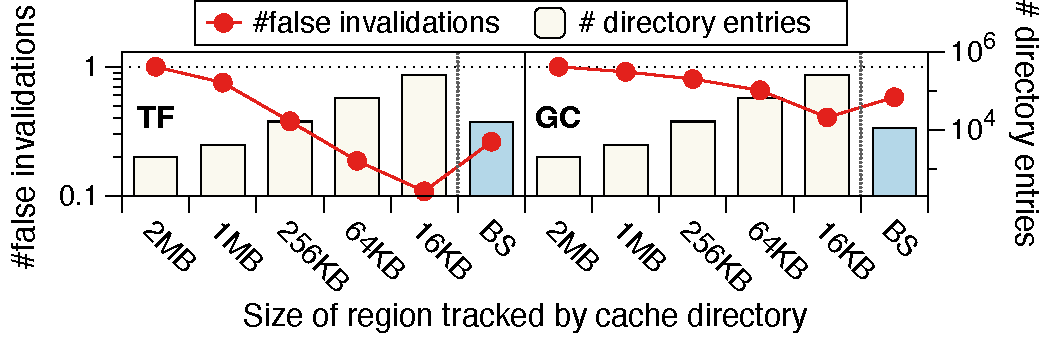
\includegraphics[width=0.49\textwidth]{fig/mind/14d_static_entries}\hspace{2em}
  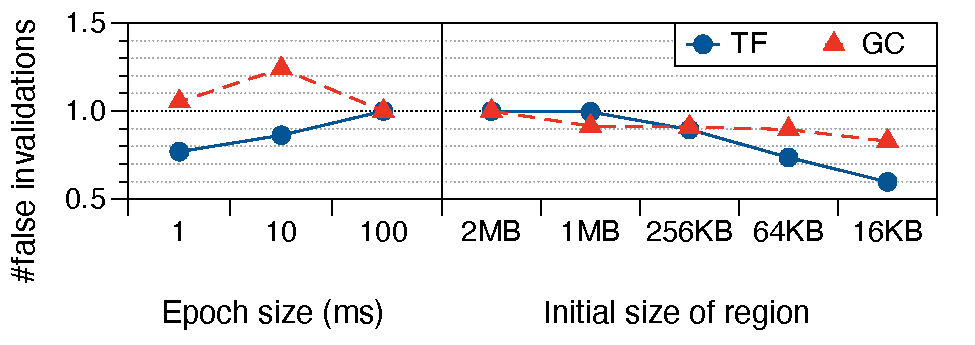
\includegraphics[width=0.46\textwidth]{fig/mind/14c_cache_tradeoff}
  \vspace{-0.9em}
  \caption[Evaluating \mind's \mindalgo algorithm.]{\textbf{Evaluating \mind's \mindalgo algorithm.} (left) Navigating switch storage vs. performance tradeoff. (right) Impact of epoch \& initial region sizing. The number of false invalidations is normalized by value at $2$~MB for region size and $100$~ms for epoch size.}
  \label{fig:storagevperf}
  \label{fig:epoch_size}
  \label{fig:region_size}
\end{figure*}%

\paragraphb{Latency for cache state transitions} Figure~\ref{fig:micro_latency} shows the end-to-end latency due to every possible state transition under the MSI protocol in \mind, including the time required to fetch the data. Note that this figure only shows latency for remote accesses --- local accesses only incur DRAM latency ($<100$~ns). On the x-axis, $2$ -- $8$C indicate the number of CPU blades requesting the same page, and $x \rightarrow y$ denotes the state transition, $x$ and $y$ being the initial and final states. 

When a blade requests read-only (shared, \textbf{S}) mode for a region, and its initial state was either invalid (\textbf{I}) or shared (\textbf{S}), it does not require any invalidations. Consequently, the data fetch can be performed in a single RDMA request (${\sim} 9~\mu$s), as seen in the first four bars. If the transition for a region is either from or to the modified (\textbf{M}) state, the requesting blade must wait until the regions is invalidated at all its previous owners. When transitioning from \textbf{S} to \textbf{M}, the data can be fetched directly from the memory blade via one-sided RDMA operation, while the invalidation at other blades occur in parallel, resulting in a total latency of ${\sim} 9~\mu$s. When the region is initially in \textbf{M} state, the (dirty) data must be fetched from and the region invalidated at the same blade --- its current owner. Therefore, the invalidation and data fetch occur sequentially, resulting in ${\sim} 18~\mu$s latency. Note that since the latency for requests with invalidations is $2\times$ higher than requests without them, a workload's performance depends on the relative proportion of the different types of requests, as we show next.

\paragraphb{Impact of invalidations on memory throughput} Figure~\ref{fig:micro_band}~(right) shows \mind memory throughput across 8 compute blades, running 1 compute thread each, under various read-write and sharing characteristics. We use read ratio to denote the fraction of reads in the workload (remaining accesses are writes), and sharing ratio to denote the portion of memory accesses that occur to a shared region (shared by all threads). We used a total working set size of $400~k$ pages, with the access pattern across them being uniform random. If most accesses are reads, then compute blades can share the same region without triggering invalidations (\textbf{S}$\rightarrow$\textbf{S} in Figure~\ref{fig:micro_latency}). As such, at read-ratio $1$, most of the pages are accessed locally from the cache, resulting in very high memory throughput ($1$-$2\times 10^{6}$ IOPS) for all sharing ratios. Again, at sharing ratio $0$, memory throughput remains high, since accessed pages can remain cached at the compute blade without being invalidated, \ie, most accesses are local. If both the write proportion and sharing ratio are increased, memory throughput drops (by ${\sim} 10\times$ at sharing-ratio $1$), since they trigger a large number number of \textbf{M}$\rightarrow$\textbf{S}, \textbf{S}$\rightarrow$\textbf{M} transitions with invalidations and permit few pages to be accessed locally.

\paragraphb{Cache directory storage} Figure~\ref{fig:macro_cache_dir}~(left) shows the number of cache directory entries stored in the switch data plane in \mind over time for the workloads evaluated in \S\ref{subsec:macro_bench} across 8 compute blades, running 10 threads each. In \mind, we fix the total amount of storage allocated to directory storage to $30$~k entries. For the TF and GC workloads, \mind's \mindalgo algorithm ensures that the number of directory entries remains well below the limit over time. However, the MC$_{A}$ and MC$_{B}$ workloads have a significantly larger number of shared memory regions, with frequent read and write accesses to them; as a consequence, the number of directory entries for the workloads always remains close to the $30$~k limit. Recall from \S\ref{subsec:macro_bench} that one of the key reasons for poor scalability of these workloads is the number of false invalidations triggered due to the relatively coarse granularity of tracking directory entries --- we believe with future switch ASICs likely to be equipped with more TCAM/SRAM, this bottleneck would no longer exist, permitting more efficient scaling under \mind.

\paragraphb{Address translation \& memory protection storage} We study the switch storage overheads due to address translation and memory protection on a setup with 8 memory blades, running the TF, GC, and M$_{A/C}$ workloads; we group $M_A$ and $M_C$ since they have the same memory allocations. Figure~\ref{fig:micro_num_entry}~(center) shows that the number of match action rules due to address translation and memory protection in \mind is almost constant, even as the workload size increases. This is due to \mind's per-memory blade partitioning of the address space, and \code{vma} granularity tracking of memory protection entries. While we have only shown results for three different applications, we find that the number of \code{vma} entries for typical datacenter applications falls in similar ranges, and well under $1$--$2$~k~\cite{vma1, vma2}. In contrast, the number of match-action rules increases linearly with the dataset size for page-based approaches, despite smaller absolute overheads with $1$~GB huge pages. Note that the upper-limit for match-action rules that the switch can store is about $45$~k --- higher than the $30$~k limit for directory entries due to a more compact representation.

\mind's memory allocation also ensures balanced placement of load across memory blades (\S\ref{subsec:addr_trans}), as shown via Jain's fairness index metric~\cite{jain} in Figure~\ref{fig:micro_load_balance}~(right). While $2$~MB pages can achieve similar load-balancing, they do so at the cost of much larger number of address translation entries. $1$~GB pages, on the other hand, observes poor load balancing for allocation-intensive workloads (M$_{A/C}$).

\subsection{Evaluating \mind's \mindAlgo Algorithm}
\label{ssec:mindsensitivity}

We now evaluate \mind's \mindalgo algorithm.

\paragraphb{Storage vs. performance tradeoff} Recall from \S\ref{ssec:caching} that the granularity at which the directory tracks memory regions exposes a tradeoff between the false invalidation count and the size of the directory itself --- Figure~\ref{fig:storagevperf}~(left) highlights this tradeoff for the TF and GC workloads. Specifically, tracking smaller regions (\eg, $16$~kB) permits fewer false invalidations, but at the cost of larger number of directory entries at the switch, while tracking larger regions (\eg, $2$~MB) exposes the opposite tradeoff. \mind's \mindalgo algorithm employs adaptive region sizing to balance both the number of directory entries as well false invalidations.

\paragraphb{Impact of epoch and initial region sizing} Figure~\ref{fig:epoch_size}~(right) shows the impact of epoch size on the total number of false invalidations for TF and GC workloads. Increasing the epoch size from $1$ to $100$~ms does not have a significant impact on the number of false invalidations, but reduces the control plane overheads. Epoch size smaller than $1$ms (not shown) are unable to capture enough invalidations to enable accurate estimation of the distribution, resulting spurious merges/splits and unpredictable false invalidations. We use $100$~ms as our default epoch size since it offers a sweet spot for minimizing both false invalidations and control plane overheads.

Figure~\ref{fig:region_size}~(right) shows that picking smaller initial region sizes results in fewer false invalidations --- intuitively, this is because larger initial region sizes require several splits before stabilizing to the appropriate region size, incurring several false invalidations in the interim. We select $16$KB as our default initial region size, since smaller region sizes result in too many directory entries during initialization. 

Finally, we note that neither parameter has any noticeable impact on the number of directory entries at stable state.

% !TEX root = ../paper.tex
\section{Limitations and Future Research}
\label{sec:discussion}

We now discuss the limitations of current \mind implementation, and future research directions to resolve them. 

\paragraphb{Thread management} Even with our optimizations, remote memory access latency is still at least two orders of magnitude higher than local latency. While our work explores in-network approaches to minimize overheads of coherence, an orthogonal approach of co-locating threads with higher proportion of shared memory accesses could yield significant improvements in end-to-end application performance by reducing the number of invalidations over the network.

\paragraphb{Other coherence protocols} While \mind implements the simple MSI coherence protocol, more complex protocols like MOESI may offer better scalability by reducing broadcasts and write-backs to disaggregated memory. Realizing such protocols would require storing larger state transition tables (STT) at the switch and handling more transient states, adding implementation complexity for ensuring correctness. Still, the number of TCAM entries required for STT entries would be quite small (\eg, tens of states for MOESI) relative to switch ASIC capacities, making them realizable today.

\paragraphb{Weaker consistency models} As we noted in \S\ref{sec:impl} and \S\ref{sec:evaluation}, our page-fault based implementation on x86 architectures cannot realize weaker consistency models like PSO. To this end, a redesign of the compute blade architecture --- \eg, by enabling page-faults on reads (but not writes) to a page --- could enable realization of weaker consistency models in \mind, facilitating higher throughput to disaggregated memory.

\paragraphb{Scaling beyond a rack} While \mind targets a rack-scale design with a single switch, some workloads may want to scale transparently beyond a single rack. This requires a shift similar to the shift from single node CPUs (akin to the rack in our setting) to multi-node NUMA architectures (akin to datacenter-scale memory disaggregation). Such a design would require extension of \mind design from a single switch to a datacenter-wide network topology.

\paragraphb{Virtualization} While \mind enables protection at a virtual memory level, extensions to virtualization are needed to facilitate true isolation across users for security, resource management, legacy OS support, \etc~Providing performance isolation, in particular, would require isolating several different shared resources along the compute-memory interconnect, including network bandwidth, switch and NIC resources.

% !TEX root = ../paper.tex
\section{Related Work}
\label{sec:related}

While we discussed prior disaggregated memory approaches in \S\ref{ssec:challenges}, we now discuss other work related to \mind. 

\paragraphb{In-network computing} There have been several recent efforts that leverage in-network computing for performance gains~\cite{innetwork, pktsched, congestion1, congestion2, lb1, lb2, netpaxos, p4xos, nopaxos, synchrony, concurrency1, concurrency2, netlock, agg1, agg2, agg3, qp1, qp2}. Most focus was on offloading \textit{application} logic and state to the network, \eg, key-value caches~\cite{netcache, incbricks} and metadata~\cite{pegasus}. Perhaps the most relevant to \mind are NOPaxos~\cite{nopaxos} and Concordia~\cite{concordia}. NOPaxos leverages the network to order requests for Paxos-based consensus, enabling consistent replication without expensive coordination overheads. While \mind targets a complementary goal of in-network memory management, it could leverage NOPaxos to enable consistent replication of disaggregated memory. Concordia, on the other hand, uses the programmable switch as a cache for directory entries in a DSM; in contrast, \mind realizes memory management completely in the network.

\paragraphb{Application-driven memory disaggregation} Recent work argues for OSes to expose resource management abstractions like memory placement and failures to the applications for high performance and better fault-tolerance~\cite{disaggapp, disaggfault}. While \mind argues for a transparent disaggregated shared memory, it is not incompatible with the above approaches --- OS-level libraries layered atop \mind could still expose memory placement and failure notifications to applications. 

Clover~\cite{clover} explores the design of a key-value store closely integrated with disaggregated persistent memory. In contrast to \mindx's in-network transparent memory management, Clover focuses on lock-free consistent access to KV pairs stored in network-attached memory using atomic RDMA verbs. While a possible design considered in~\cite{clover} places key-value coordination and access logic at a centralized coordinator, it does not place the logic in the network fabric and does not consider memory protection, caching or coherence.

\paragraphb{Emerging industry standards} While most industry standards for high performance compute-memory interconnects like CCIX~\cite{ccix}, CXL~\cite{cxl} and OpenCAPI~\cite{opencapi} target \textit{intra}-server settings, Gen-Z~\cite{genz} is perhaps the closest to \mind since it targets \textit{inter}-server fabrics. The Gen-Z standard defines operations like \code{ExclusiveRead} and \code{Writeback} that may be used as building blocks for software-based coherence~\cite{genz, genz1}, although we are unaware of any publicly available realization. Moreover, the MMU functionalities in all the above industry standards are realized at the \textit{endpoints}, \eg, at specialized ZMMUs at CPU and memory nodes in Gen-Z; the \textit{fabric} (\eg, the switch) only forwards memory requests and responses. This is in contrast to \mind's approach of in-network memory management, \ie, \mind's design is complementary to the industry efforts towards high-performance interconnects.

% !TEX root = ../paper.tex
\section{Conclusion}

We have presented \mind, an in-network memory management unit for rack-scale memory disaggregation. \mind achieves resource elasticity, performance and transparency through a principled redesign of traditional memory management mechanisms to achieve their individual goals in the disaggregated setting while operating under programmable switch ASIC resource constraints. Our \mind prototype facilitates transparent resource elasticity, while matching the performance of prior memory disaggregation proposals for real-world workloads.



%\subsection{Introduction}
%The current state of data center network bandwidth is rapidly approaching parity with intraserver resource interconnects, with projections indicating an imminent surpassing of this threshold. This dynamic shift has ignited considerable interest within both academic and industrial circles towards memory disaggregation—a paradigm where compute and memory are physically decoupled into network-attached resource blades. This transformation promises to revolutionize resource utilization, hardware diversity, resource scalability, and fault tolerance compared to conventional data center architectures.
%
%However, memory disaggregation presents formidable challenges, primarily revolving around three key requisites. Firstly, remote memory access demands low latency and high throughput, with previous studies targeting latency under 10 microseconds and bandwidth exceeding 100 Gbps per compute blade to minimize performance degradation in applications. Secondly, both memory and compute resources must exhibit elastic scalability, aligning with the essence of disaggregation. Lastly, seamless adoption and immediate deployment necessitate compatibility with unaltered applications.
%
%Despite years of concerted research efforts directed towards enabling memory disaggregation, existing approaches have failed to concurrently meet all three requirements. Most strategies mandate application modifications due to alterations in hardware, programming models, or memory interfaces. Recent endeavors facilitating transparent access to disaggregated memory have encountered limitations on application compute elasticity—processes are confined to compute resources on a single blade to mitigate cache coherence traffic over the network, driven by performance apprehensions.
%
%Introducing MIND, a pioneering memory management system tailored for rack-scale memory disaggregation, which effectively fulfills all three prerequisites for disaggregated memory. At the core of MIND lies a novel concept—embedding memory management logic and metadata within the network fabric. This innovative approach capitalizes on the insight that the network fabric in a disaggregated memory architecture essentially functions as a CPU-memory interconnect. In MIND, programmable network switches, strategically positioned for in-network processing, assume the mantle of Memory Management Units (MMUs), enabling a high-performance shared memory abstraction. Leveraging programmable hardware at line rate, MIND minimizes latency and bandwidth overheads.
%
%However, the realization of in-network memory management necessitates navigating through the unique constraints imposed by programmable switch ASICs. These challenges include limited on-chip memory capacity, constraints on computational cycles per packet, and staged packet processing pipelines spread across physically decoupled match-action stages.
%
%To address the trifecta of requirements for memory disaggregation, MIND ingeniously maneuvers through these constraints and harnesses the capabilities of contemporary programmable switches to enable in-network memory management for disaggregated architectures. This is achieved through a systematic overhaul of traditional memory management mechanisms:
%
%MIND adopts a globally shared virtual address space, partitioned across memory blades to minimize the volume of address translation entries stored in the on-chip memory of switch ASICs. Simultaneously, it implements a physical memory allocation mechanism that evenly distributes allocations across memory blades for optimal memory throughput.
%
%MIND incorporates domain-based memory protection, inspired by capability-based schemes, facilitating fine-grained and flexible protection by dissociating the storage of memory permissions from address translation entries. Interestingly, this decoupling reduces on-chip memory overheads in switch ASICs.
%
%MIND adapts directory-based MSI coherence to the in-network setting, leveraging network-centric hardware primitives like multicast in switch ASICs to efficiently realize its coherence protocol.
%
%To mitigate the performance impact of coarse-grained cache directory tracking due to limited on-chip memory in switch ASICs, MIND introduces a novel Bounded Splitting algorithm that dynamically sizes memory regions to constrain both switch storage requirements and performance overheads stemming from false invalidations.
%
%The MIND design is realized on a disaggregated cluster emulated using traditional servers connected by a programmable switch. Results demonstrate that MIND facilitates transparent resource elasticity for real-world workloads while matching or even surpassing the performance of prior memory disaggregation proposals. However, it's noted that workloads characterized by high read-write contention exhibit sub-linear scaling with additional threads due to the limitations of current hardware. Present x86 architectures hinder the implementation of relaxed consistency models commonly employed in shared memory systems, and the switch TCAM capacity nears saturation with cache directory entries for such workloads. Potential approaches for enhancing scalability with future advancements in switch ASIC and compute blade architectures are discussed.
%\subsection{Background and Motivation}
%This section motivates MIND. We discuss key enabling technologies, followed by challenges in realizing memory disaggregation goals using existing designs.
%
%Assumptions: We focus on memory disaggregation at the rack-scale, where memory and compute blades are connected by a single programmable switch. We restrict our scope to partial memory disaggregation: while most of the memory is network-attached, CPU blades possess a small amount (few GBs) of local DRAM as cache.
%
%2.1 Enabling Technologies
%We now briefly describe MIND’s enabling technologies.
%
%Programmable switches: In recent years, programmable switches have evolved along two well-coordinated directions: development of a flexible programming language for network switches and the design of switch hardware that can be programmed with it. These switches host an application-specific integrated circuit (ASIC), along with a general-purpose CPU with DRAM. The switch ASIC comprises ingress pipelines, a traffic manager, and egress pipelines, which process packets in that order. Programmability is facilitated through a programmable parser and match-action units in the ingress/egress pipelines.
%
%The program defines how the parser parses packet headers to extract a set of fields, and multiple stages of match-action units process them. The general-purpose CPU is connected to the switch ASIC via a PCIe interface and serves two functions: (i) performing packet processing that cannot be performed in the ASIC due to resource constraints, and, (ii) hosting controller functions that compute network-wide policies and push them to the switch ASIC.
%
%While this discussion focuses on switch ASICs with Reconfigurable Match Action Tables (RMTs), it is possible to realize MIND using FPGAs, custom ASICs, or even general-purpose CPUs. Each exposes different tradeoffs, but we adopt RMT switches due to their performance, availability, power, and cost efficiency.
%
%DSM Designs: Traditionally, shared memory has been explored in the context of NUMA and distributed shared memory (DSM) architectures. In such designs, the virtual address space is partitioned across the various nodes, i.e., each partition has a home node that manages its metadata, e.g., the page table. Each node also has a cache to facilitate performance for frequently accessed memory blocks. We distinguish memory blocks from pages since caching granularities can be different from memory access granularities.
%
%With the copies of blocks potentially residing across multiple node caches, coherence protocols are required to ensure each node operates on the latest version of a block. In popular directory-based invalidation protocols like MSI (used in MIND), each memory block can be in one of three states: Modified (M), where a single node has exclusive read and write access to the block; Shared (S), where one or more caches have shared read-only access to the block; and Invalid (I), where the block is not present in any cache. A directory tracks the state of each block, along with the list of nodes that currently hold the block in their cache. The directory is typically partitioned across the various nodes, with each home node tracking directory entries for its own address space partition. Memory access for a block that is not local involves contacting the home node for the block, triggering a state transition and potential invalidation of the block across other nodes, followed by retrieving the block from the node that owns it.
%
%While it is possible to realize more sophisticated coherence protocols, we restrict our focus to MSI in this work due to its simplicity.
%
%As outlined earlier, extending the benefits of resource disaggregation to memory and making them widely applicable to cloud services demands (i) low-latency and high-throughput access to memory, and (ii) a transparent memory abstraction that supports elastic scaling of memory and compute resources without requiring modifications to existing applications. Unfortunately, prior designs for memory disaggregation expose a hard tradeoff between these two goals. Specifically, transparent elastic scaling of an application’s compute resources necessitates a shared memory abstraction over the disaggregated memory pool, which imposes non-trivial performance overheads due to the cache-coherence required for both application data and memory management metadata. We now discuss why this tradeoff is fundamental to existing designs. We focus on page-based memory disaggregation designs here.
%
%Transparent designs: While transparent distributed shared memories (DSMs) have been studied for several decades, their adaptation to disaggregated memory has not been explored. We consider two possible adaptations for the approach outlined earlier to understand their performance overheads and shed light on why they have remained unexplored thus far. The first is a compute-centric approach, where each compute blade owns a partition of the address space and manages the corresponding metadata, but the memory itself is disaggregated. A compute blade must now wait for several sequential remote requests to be completed for every un-cached memory read or write, for example, to the remote home compute blade to trigger state transition for the block and invalidate relevant blades, and to fetch the memory block from the blade that currently owns the block.
%
%An alternate memory-centric design that places metadata at corresponding home memory blades still suffers multiple sequential remote requests for a memory access as before, with the only difference being that the home node accesses are now directed to memory blades. While these overheads can be reduced by caching the metadata at compute blades, it necessitates coherence for the metadata as well, incurring additional design complexity and performance overheads.
%
%Non-transparent designs: Due to the anticipated overheads of adapting DSM to memory disaggregation, existing proposals limit processes to a single compute blade, i.e., while compute blades cache data locally, different compute blades do not share memory to avoid sending coherence messages over the network. As such, these proposals achieve memory performance only by limiting transparent compute elasticity for an application to the resources available on a single compute blade, requiring application modifications if they wish to scale beyond a compute blade.
%
%\subsection{MIND Design}
%To break the tradeoff highlighted above, we place memory management in the network fabric for three reasons. First, the network fabric enjoys a central location in the disaggregated architecture. Therefore, placing memory management in the data access path between compute and memory resources obviates the need for metadata coherence. Second, modern network switches permit the implementation of such logic in integrated programmable ASICs. These ASICs are capable of executing at line rate even for multi-terabit traffic. In fact, many memory management functionalities have similar counterparts in networking, allowing us to leverage decades of innovation in network hardware and protocol design for disaggregated memory management.
%
%Finally, placing the cache coherence logic and directory in the network switch permits the design of specialized in-network coherence protocols with reduced network latency and bandwidth overheads. Effective in-network memory management requires: (i) efficient storage by minimizing in-network metadata given the limited memory on the switch data plane; (ii) high memory throughput by load-balancing memory traffic across memory blades; and (iii) low access latency to shared memory via efficient cache coherence design that hides the network latency.
%
%Next, we elicit three design principles followed by MIND to realize the above goals and provide an overview of its design.
%
%\subsubsection{MIND Design Principles}
%MIND adheres to three key principles to achieve the memory disaggregation goals outlined earlier:
%
%P1: Decouple memory management functionalities to allow each to be optimized for its specific objectives.
%P2: Utilize a centralized control plane's global view of the disaggregated memory subsystem to compute optimal policies for each memory management functionality.
%P3: Leverage network-centric hardware primitives within the programmable switch ASIC to efficiently implement the policies determined by P2.
%MIND applies P1 by separating memory allocation from addressing, address translation from memory protection, and cache access and eviction from coherence protocol execution. P2 and P3 are employed to efficiently realize these objectives. Traditional server-based operating systems, however, are unable to take advantage of these principles due to their reliance on fixed-function hardware modules, such as the MMU and memory controller, which typically couple various memory management tasks (e.g., address translation and memory protection in page-table walkers) for reasons of complexity, performance, and power efficiency.
%
%\subsubsection{Overview}
%MIND provides a transparent virtual memory abstraction to applications, similar to traditional server-based OSes. However, unlike previous disaggregated memory designs, MIND places all memory management logic and metadata in the network, rather than on CPU or memory blades, or a separate global controller.
%
%In MIND's design, CPU blades run user processes and threads and possess a small amount of local DRAM used as a cache. Memory allocations and deallocations from user processes are intercepted at the CPU blade and forwarded to the switch control plane. The control plane, which has a global view of the system, performs memory allocations, assigns permissions, and responds to user processes. All memory load/store operations are handled by the CPU blade's cache. This cache is virtually addressed and stores permissions to enforce memory protection. If a page is not cached locally, a page fault is triggered, causing the CPU blade to fetch the page from memory blades using RDMA requests, evicting other cached pages if necessary. If a memory access requires a coherence state update (e.g., a store on a shared block), a page fault triggers the cache coherence logic at the switch.
%
%MIND performs page-level remote accesses due to its page-fault-based design, although future CPU architectures may support more flexible access granularities. Since CPU blades do not store memory management metadata, the RDMA requests contain only virtual addresses, without any endpoint information for the memory blade holding the page. The switch data plane intercepts these requests, handles cache coherence by updating the cache directory, and performs cache invalidations on other CPU blades. It also ensures that the requesting process has the appropriate permissions. If no CPU blade cache holds the page, the data plane translates the virtual address to a physical one and forwards the request to the appropriate memory blade.
%
%In this design, memory blades merely store the actual memory pages and serve RDMA requests for physical pages. Unlike earlier approaches that rely on RPC handlers and polling threads, MIND uses one-sided RDMA operations to eliminate the need for CPU cycles on disaggregated memory blades, moving towards true hardware resource disaggregation where memory blades do not need general-purpose CPUs.
%Placing memory management logic and metadata in the network enables simultaneous optimization for both memory performance and resource elasticity. We now explain how MIND optimizes for the goals of memory allocation and addressing, memory protection, and cache coherence, while adhering to the constraints of programmable switches. We also discuss how MIND handles failures.
%
%4.1 Memory Allocation \& Addressing
%Traditional virtual memory uses fixed-sized pages as basic units for translation and protection, which can lead to inefficiencies in storage due to memory fragmentation. Smaller pages reduce fragmentation but require more translation entries, and larger pages have the opposite effect. To address this, MIND decouples address translation from protection. MIND's translation is blade-based, while protection is virtual memory area (vma)-based.
%
%Storage-efficient address translation: MIND avoids page-based protection and instead uses a single global virtual address space across all processes, allowing shared translation entries. MIND partitions the virtual address space across different memory blades, mapping each blade’s portion to a contiguous physical address range. This approach reduces the storage needed for translation entries in the switch's data plane. The mapping is adjusted when memory blades are added, removed, or when memory is moved.
%
%Balanced memory allocation \& reduced fragmentation: The control plane tracks total memory allocation across blades and places new allocations on blades with the least allocation, achieving load balancing. Additionally, MIND minimizes fragmentation within each memory blade by using traditional virtual memory allocation schemes, resulting in virtual memory areas (vmas) that are non-overlapping, reducing fragmentation.
%
%Isolation: MIND's global virtual address space does not compromise process isolation. The switch control plane intercepts all allocation requests and ensures that they do not overlap between processes. MIND's vma-based protection allows for flexible access control within a global virtual address space.
%
%Support for static virtual addresses: MIND supports unmodified applications with static virtual addresses embedded in their binaries or OS optimizations like page migration. It maintains separate range-based address translations for static virtual addresses or migrated memory, ensuring correctness through longest-prefix matching in the switch’s TCAM.
%
%4.2 Memory Protection
%MIND decouples translation from protection by using a separate table to store memory protection entries in the data plane. Applications can assign access permissions to vmas of any size, and the protection table stores entries for these vmas. This flexible protection system allows MIND to efficiently manage memory protection with a relatively small number of entries.
%
%Fine-grained, flexible memory protection: MIND introduces two abstractions: protection domains and permission classes. Protection domains define which entities can access a memory region, while permission classes specify the types of access allowed. MIND’s control plane provides APIs that allow applications to assign protection domains and permission classes to vmas. These entries are stored in the protection table, and MIND efficiently supports this matching using TCAM-based range matches in the switch ASIC.
%
%Optimizing for TCAM storage: MIND ensures storage efficiency by aligning virtual address allocations to power-of-two sizes, allowing regions to be represented using a single TCAM entry. Adjacent entries with the same protection domain and permission class are coalesced to further reduce storage requirements.
%
%4.3 Caching \& Cache Coherence
%In MIND, caches reside on compute blades, while the coherence directory and logic are located in the switch. This placement reduces latency for coherence protocol execution. MIND addresses challenges in adapting traditional cache management to an in-network setting by decoupling cache and directory granularities and dynamically optimizing region sizes.
%
%Decoupling cache access \& directory entry granularities: MIND decouples cache access from directory entry granularity. Cache accesses and memory movements are performed at fine granularities (e.g., 4 KB pages), while directory entries are tracked at larger, variable-sized regions. Invalidation of a region triggers the invalidation of all dirty pages tracked by the CPU blade caches.
%
%Storage \& performance-efficient sizing of regions: MIND uses the global view of memory traffic at the switch control plane to dynamically adjust region sizes, balancing between performance (minimizing false invalidations) and directory storage efficiency.
%
%4.4 Handling Failures
%MIND leverages prior work to handle CPU and memory blade failures. For switch failures, the control plane is consistently replicated at a backup switch, ensuring that data plane state can be reconstructed.
%
%Communication failures: MIND uses ACKs and timeouts to detect packet losses. In case of a timeout during invalidation, the compute blade sends a reset message to the control plane, which flushes the data and removes the corresponding cache directory entry, preventing deadlocks during state transitions.
%
%\subsubsection{In-Network Memory Management}
%
%\subsection{MIND Implementation}
%MIND Implementation
%MIND integrates with the Linux memory and process management system call APIs and splits its kernel components across CPU blades and the programmable switch. We will now describe these kernel components, along with the RDMA logic required for the memory blades.
%
%6.1 CPU Blade
%MIND uses a partial disaggregation model, where CPU blades have a small amount of local DRAM that acts as a cache. In our prototype, traditional servers are used for the CPU blades, with no hardware modifications. We implemented MIND’s CPU blade kernel components as modifications to the Linux 4.15 kernel, providing transparent access to disaggregated memory by modifying how vmas and processes are managed and how page faults are handled.
%
%Managing vmas: The kernel module intercepts process heap allocation and deallocation requests, such as brk, mmap, and munmap, forwarding them to the control plane at the switch over a reliable TCP connection. The switch creates new vma entries and returns the corresponding values (e.g., the virtual address of the allocated vma), ensuring transparency for user applications. Error codes like ENOMEM are returned for errors, similar to standard Linux system calls.
%
%Managing processes: The kernel module also intercepts and forwards process creation and termination requests, such as exec and exit, to the switch control plane, which maintains internal process representations (i.e., Linux’s task\_struct) and manages the mapping between compute blades and the processes they host. Threads across CPU blades are assigned the same PID if they belong to the same process, enabling them to share the same address space transparently through the memory protection and address translation rules installed at the switch. We place threads and processes across compute blades in a round-robin fashion without focusing on scheduling.
%
%Page fault-driven access to remote memory: When a user application attempts to access a memory address not present in the CPU blade cache, a page fault handler is triggered. The CPU blade sends a one-sided RDMA read request to the switch with the virtual address and requested permission class (read or write). The page is registered to the NIC as the receiving buffer, eliminating the need for additional data copies. Once the page is received, the local memory structures are populated, and control is returned to the user. The CPU blade DRAM cache handles cache invalidations for coherence, tracking writable pages locally and flushing them when receiving invalidation requests.
%
%This approach provides transparent access to disaggregated memory but restricts MIND to a stronger Total Store Order (TSO) memory consistency model. Weaker consistency models, such as Process Store Order (PSO), which allow asynchronous propagation of writes, are challenging to implement on traditional x86 and ARM architectures due to the inability to trigger page faults only on reads without also triggering them on writes. This limitation affects scalability for workloads with high read/write contention to shared memory regions.
%
%6.2 Memory Blade
%MIND does not require any compute or data plane processing logic on memory blades, eliminating the need for general-purpose CPUs. In our prototype, memory blades are traditional Linux servers, so we use a kernel module to perform RDMA-specific initializations. When a memory blade comes online, its kernel registers physical memory addresses to the RDMA NIC and reports them to the global controller. After this, one-sided RDMA requests from CPU blades are handled directly by the memory blade NIC without CPU involvement. Ideally, future memory blades could be fully implemented in hardware, without requiring a CPU, to reduce costs and simplify design.
%
%6.3 Programmable Switch
%MIND’s programmable switch is implemented on a 32-port EdgeCore Wedge switch with a 6.4 Tbps Tofino ASIC, an Intel Broadwell processor, 8 GB of RAM, and 128 GB of SSD storage. The general-purpose CPU hosts the MIND control program, handling process, memory, and cache directory management, while the ASIC performs address translation, memory protection, directory state transitions, and virtualizes RDMA connections between compute and memory blades.
%
%Process \& memory management: The control plane hosts a TCP server to handle system call intercepts from CPU blades and maintains traditional Linux data structures for process and memory management. Upon receiving a system call, the control plane updates these structures and responds with system call return values to maintain transparency.
%
%Cache directory management: MIND reserves SRAM at the switch’s data plane for directory entries, partitioned into fixed-size slots, one per memory region. The control plane maintains a free list of available slots and a hash table mapping base virtual addresses of cache regions to their corresponding directory entries in the SRAM. When a directory entry is created or a region is split, slots are allocated or deallocated as needed. Directory state transitions are handled across multiple match-action units (MAUs) due to limited compute capabilities in each unit, with state transitions split between them and recirculating the packet within the switch data plane as needed.
%
%Virtualizing RDMA connections: MIND virtualizes RDMA connections between all possible CPU and memory blade pairs by transforming and redirecting RDMA requests and responses. Once a request’s destination is identified through address translation or cache coherence, the switch updates the packet header fields (IP/MAC addresses and RDMA parameters) before forwarding the request to the correct memory blade.
%
%
%\subsection{Evaluation}
%\subsection{Discussion and Conclusion}
%%\label{ssec:MIND}
%\begin{comment}
%
%\begin{figure*}[t]
%    \centering
%    \subfigure[MIND architecture]{
%      \includegraphics[width=0.60\textwidth]{fig/mind.pdf}
%      \label{fig:mind}}
%    \subfigure[MIND dataflow]{
%      \includegraphics[width=0.37\textwidth]{fig/mindflow.pdf}
%    \label{fig:mindflow}}\vspace{-1.0em}
%      \caption{\textbf{MIND overview} (a) Each CXL server is equipped with two A1000 memory expansion cards. (b) Our platform comprises two CXL servers and one baseline server. The baseline server replicates the same configuration but lacks any CXL memory cards.}\vspace{-1.0em}
%\end{figure*}
%    
%\end{comment}
%We start at a relatively modest scale, specifically within the context of rack-scale~\cite{industry2, industry4}. Our perspective aligns with placing the operating system functionality for non-disaggregated resources within the interconnect, which serves as the network infrastructure in a rack-scale system (or potentially utilizing CXL, as discussed in \S\ref{sec:hardware}). The advantage of housing this functionality in the interconnect is it grants the system a global view, as every compute-memory operation must traverse the interconnect.
%
%
%The network emerges as a compelling choice for an interconnect in memory disaggregation due to several key factors. First, the expansion of network bandwidth surpassing that of memory bandwidth~\cite{terabitethernet} positions it as a prime candidate for serving as a disaggregation interconnect. Furthermore, advancements in programmable networking, exemplified by programmable switches~\cite{progswitch1,progswitch2,progswitch3, progswitch4}, enable capabilities such as data storage (state-keeping) and processing at line-rate~\cite{pktsched}. These capabilities empower the network to implement critical OS functionality effectively.
%
%
%There are several essential requirements for memory management within a disaggregated architecture. Firstly, the interconnect operating system must operate without additional overhead, ensuring minimal latency and facilitating high-throughput access to remote memory. Additionally, given that programs may utilize various resources across compute and memory blades, the operating system should enable elastic scaling for both memory and computational resources. Another advantageous aspect of housing OS functionality within the interconnects is the ability to shield the application entirely from the OS logic, thereby promoting compatibility with unmodified applications.
%
%To fulfill the three essential requirements, we have developed a system known as MIND~\cite{mind}, leveraging the capabilities of contemporary programmable switches to facilitate in-network memory management. Drawing inspiration from the similarity between memory address translation and network address lookups, we utilize the existing ingress/egress pipelines and Reconfigurable Match Action Tables (RMTs)\cite{rmt} within programmable switches to implement address translation tables and protection entries. Additionally, we implement a directory-based MSI coherence protocol\cite{msi}, as data may be accessed coherently by multiple compute nodes. These operations are performed at line rate, ensuring low-latency, high-throughput memory access. It's worth noting that our implementation is confined to the interconnect (programmable switch) and the compute node OS kernel, allowing applications to run seamlessly on MIND.
%
%Figure \ref{fig:mind} illustrates the fundamental structure of the MIND system. Compute nodes house CPUs and a limited cache, while memory nodes exclusively contain memory resources. The programmable switch is situated atop the rack, with the control plane managing coarse-grained operations like memory allocation, permission assignment, and memory coherence directory management. Meanwhile, the data plane handles memory address translation, protection, and coherence lookup at line rate.
%
%The dataflow(Figure \ref{fig:mindflow}) of memory access begins with a load/store instruction from the compute node CPU. When the compute node OS kernel detects that the required data isn't present on the node, it triggers a page fault and issues a network request to the switch for permission updates and data retrieval. This request traverses the switch's data plane, fetching the required data from the memory node. Simultaneously, the switch invalidates existing data from other compute nodes if the source node requests exclusive access.
%
%We've faced two main challenges with programmable switch ASICs: limited on-chip memory and restricted computational power. The few megabytes of memory on switch ASICs are inadequate for traditional page tables managing terabytes of disaggregated memory. Moreover, the ASICs' computational constraints, necessary for maintaining line-rate processing, are evident in complex tasks like cache coherence. To counter these issues, we've separated memory addressing and protection to save hardware space. Additionally, we've utilized unique switch primitives like multicast operations to navigate computational limitations effectively.
%
%

\section{Near Memory Processing}
%\label{ssec:Pulse}

% !TEX root = ../paper.tex
% \vspace{-0.5em}
\subsection{Introduction}



% Background
\noindent
Driven by increasing demands for memory capacity and bandwidth~\cite{scuba, cachelib, tao, memcache, flighttracker, twittercache, spark}, poor scaling~\cite{memscaling2, memscaling3, memscaling1} and resource inefficiency~\cite{infiniswap, memoverprovisioning} of DRAM, and improvements in Ethernet-based network speeds~\cite{terabitethernet, remotememory}, recent years have seen significant efforts towards memory disaggregation~\cite{fastswap, memdisagg1, infiniswap, mind, legoos}. Rather than scaling up a server's DRAM capacity and bandwidth, such proposals advocate disaggregating much of the memory over the network. The result is a set of CPU nodes equipped with a small amount of DRAM used as cache\footnote{Not to be confused with die-stacked hardware DRAM caches~\cite{jevdjic2013stacked, jevdjic2014unison, young2018accord}.}, accessing memory across a set of network-attached memory nodes with large DRAM pools (Fig.~\ref{fig:disagg}~(top)). With allocation flexibility across CPU and memory nodes, disaggregation enables high utilization and elasticity.


% Problem
Despite drastic improvements in recent years, the limited bandwidth and latency to network-attached memory remain a hurdle in adopting disaggregated memory, with speed-of-light constraints making it impossible to improve network latency beyond a point. Even with near-terabit links and hardware-assisted protocols like RDMA~\cite{rdmalatency}, remote memory accesses are an order of magnitude slower than local memory accesses~\cite{disagg}. Emerging CXL interconnects~\cite{cxl} share a similar trend --- around $300$ ns of CXL memory latency compared to $10$--$20$ ns of L3 cache latency~\cite{pond}. Although efficient caching strategies at the CPU node can reduce average memory access latency and volume of network traffic to remote memory, the benefit of such strategies is limited by data locality and the size of the cache on the CPU node. In many cases, remote memory accesses are unavoidable, especially for applications that rely on efficient in-memory pointer traversals on linked data structures, such as lookups on index structures~\cite{hash1, hash2, hash3, succinct, trie2, btree1, btree2, trie1, blowfish, trie3, surf} in databases and key-value stores, and traversals in graph analytics~\cite{powergraph, graphx, graphchi, pagerank} (Fig.~\ref{fig:motivation}, \S\ref{sec:overview}). 
\begin{figure}[t]
  \centering
  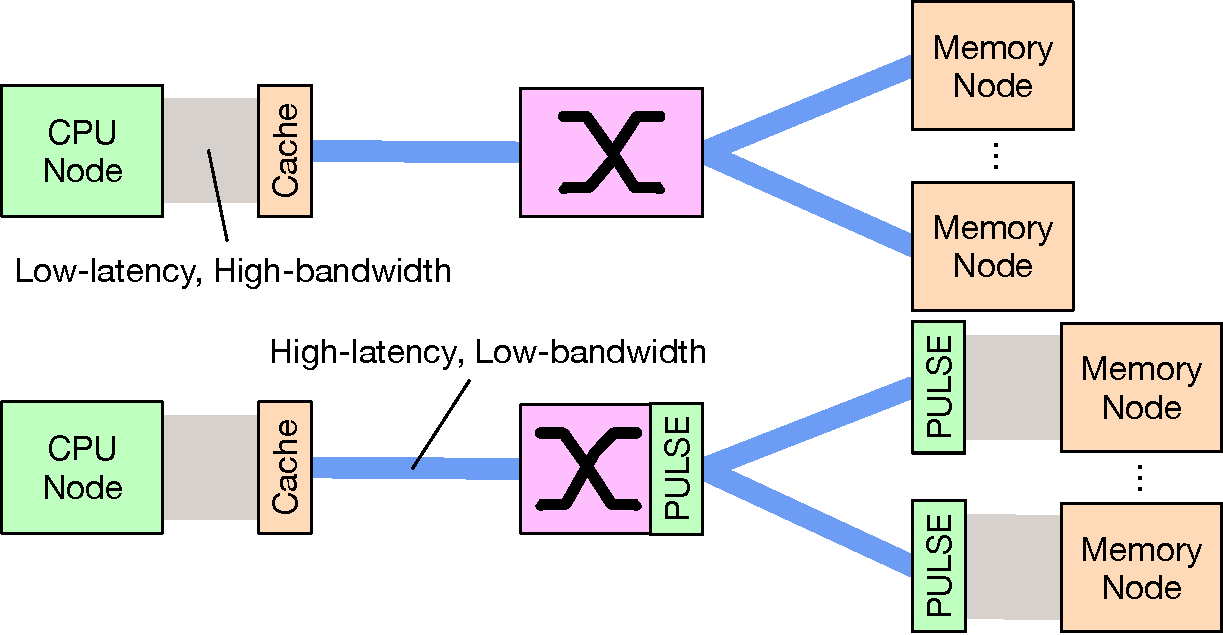
\includegraphics[width=0.98\columnwidth]{fig/pulse/disagg_vertical.pdf}
  \vspace{-0.7em}
  \caption{\textbf{Need for accelerating pointer traversals.} \textit{(top)} The performance of pointer traversals in disaggregated architectures is bottlenecked by slow memory interconnect. \textit{(bottom)} Just as caches offer limited but fast caches near CPUs, we argue that memory needs a counterpart for traversal-heavy workloads: a lightweight but fast accelerator for cache-unfriendly pointer traversals.} 
  \label{fig:disagg}%\vspace{-1.5em}
\end{figure}

\begin{figure*}[ht!]
    \centering
    \subfigure[Our empirical analysis]{
        \includegraphics[width=0.40\textwidth]{fig/pulse/figure1_motivation.pdf}
        \label{fig:motivation_experiment}
    }
    \subfigure[\% of distributed traversals]{
        \includegraphics[width=0.21\textwidth]{fig/pulse/distributed.pdf}
        %\vspace{1pt}
        \label{fig:distributed_percentage}
    }
    \subfigure[CDF of distributed traversals]{
        \includegraphics[width=0.24\textwidth]{fig/pulse/cdf.pdf}
        \label{fig:distributed_cdf_wiredtiger}
    }
    \vspace{-1em}
    \caption{\textbf{Time cloud applications spend in pointer traversals.} See \S\ref{ssec:need} for details.} 
    \label{fig:motivation}%\vspace{-1.5em}
\end{figure*}


Similar to how CPUs have small but fast memory (\ie, caches) for quick access to popular data, we argue that memory nodes should also include lightweight but fast processing units with high-bandwidth, low-latency access to memory to speed up pointer-traversals (Fig.~\ref{fig:disagg}~(bottom)). Moreover, the interconnect should facilitate efficient and scalable distributed traversals for deployments with multiple memory nodes that cater to large-scale linked data structures. Prior works have explored systems and API designs for such processing units under multiple settings, ranging from near-memory processing and processing-in-memory approaches~\cite{ahn2015scalable, asghari2016chameleon,  dai2018graphh, schuiki2018scalable, mutlu2019processing, lockerman2020livia, tu2022redcim, devic2022_PIM, wang2022_Nearstream, xie2023mpu, mutlu2022modern, oliveira2022accelerating, eckert2022eidetic, chi2016prime, seshadri2017simple, kwon2019_TensorDIMM, boroumand2019_codna, cho2020_data, ke2020_RecNMP, wang2021stream, xie2021spacea, ke2021near, singh2021fpga, olgun2022pidram, dai2022dimmining, gu2020ipim, gomez2023evaluating, walkers, impica} for single-server architectures, to the use of CPUs~\cite{storagefunctions, splinter, aifm, kayak_nsdi_21, storm_systor_19, zhang2022_teleport} or FPGAs~\cite{clio, strom} near remote/disaggregated memory, but have several key shortcomings. 


% Related work
Specifically, existing approaches are limited in scale and expose a three-way tradeoff between expressiveness, energy efficiency, and performance. First, and perhaps most crucially, none of the existing approaches can accelerate pointer traversals that span \emph{multiple} network-attached memory nodes. 

This limits memory utilization and elasticity since applications must confine their data to a single memory node to accelerate pointer traversals. Their inability to support distributed pointer traversals stems from complex management of address translation state that is required to identify if a traversal can occur locally or must be re-routed to a different memory node (\S\ref{ssec:prior}). Second, existing single-node approaches use full-fledged CPUs for expressive and performant execution of pointer-traversals~\cite{storagefunctions, splinter, aifm, kayak_nsdi_21}. However, coupling large amounts of processing capacity with memory --- which has utility in reducing data movement in PIM architectures~\cite{ahn2015scalable, dai2018graphh, schuiki2018scalable, mutlu2019processing, mutlu2022modern, oliveira2022accelerating, eckert2022eidetic, xie2023mpu, tu2022redcim, lockerman2020livia, asghari2016chameleon, devic2022_PIM, wang2022_Nearstream} ---  goes against the very spirit of memory disaggregation since it leads to poor utilization of compute resources and, consequently, poor energy efficiency. 

Approaches that use wimpy processors at SmartNICs~\cite{rmc_hotnets20, redn} instead of CPUs retain expressiveness, but the limited processing speeds of wimpy nodes curtail their performance and, ultimately lead to lower energy efficiency due to their lengthened executions (\S\ref{ssec:application-study},~\cite{clio}). Lastly, FPGA-based~\cite{clio, strom, sun2023demystifying} and ASIC-based~\cite{impica, walkers} approaches achieve performance and energy efficiency by hard-wiring pointer traversal logic for specific data structures, limiting their expressiveness.  


We design \name\footnote{\textbf{P}rocessing \textbf{U}nit for \textbf{L}inked \textbf{S}tructur\textbf{E}s.}, a distributed pointer-traversal framework for rack-scale disaggregated memory, to meet all of the above needs --- namely, expressiveness, energy efficiency, performance --- via a principled redesign of near-memory processing for disaggregated memory. Central to \name's design is an expressive iterator interface that readily lends itself to a unifying abstraction across most pointer traversals in linked data structures used in key-value stores~\cite{redis, memcached}, databases~\cite{wiredtiger, btree1, btree2, trie1, trie3}, and big-data analytics~\cite{powergraph, graphx, graphchi, pagerank} (\S\ref{sec:interface}). \name's use of this abstraction not only makes it immediately useful in this large family of real-world traversal-heavy use cases, but also enables (i) the use of familiar compiler toolchains to support these use cases with little to no application modifications and (ii) the design of tractable hardware accelerators and efficient distributed traversal mechanisms that exploit properties unique to iterator abstractions.


In particular, \name enables transparent and efficient execution of pointer traversals for our iterator abstraction via a novel accelerator that employs a \emph{disaggregated} architecture to decouple logic and memory pipelines, exploiting the inherently sequential nature of compute and memory accesses in iterator execution (\S\ref{sec:accelerator}). This permits high utilization by provisioning more memory and fewer logic pipelines to cater to memory-centric pointer traversal workloads. A scheduler breaks pointer traversal logic from multiple concurrent workloads across the two sets of pipelines and employs a novel multiplexing strategy to maximize their utilization. While our implementation leverages an FPGA-based SmartNIC due to the high cost and complexity of ASIC fabrication, our ultimate vision is an ASIC-based realization for improved performance and energy efficiency. 

We enable distributed traversals by leveraging the insight that pointer traversal across network-attached memory nodes is equivalent to packet routing at the network switch (\S\ref{sec:distributed}). As such, \name leverages a programmable network switch to inspect the next pointer to be traversed within iterator requests and determine the next memory node to which the request should be forwarded --- both at line rate. We implement a real-system prototype of \name on a disaggregated rack of commodity servers, SmartNICs, and a programmable switch with full-system effects. None of \name's hardware or software changes are invasive or overly complex, ensuring deployability.  Our evaluation of end-to-end real-world workloads shows that \name outperforms disaggregated caching systems with $9$--$34\times$ lower latency and $28$--$171\times$ higher throughput. Moreover, our Xilinx XRT~\cite{xilinx_xrt} and Intel RAPL~\cite{intel_rapl}-based power analysis shows that \name consumes $4.5$--$5\times$ less energy than RPC-based schemes (\S\ref{sec:evaluation}).

\subsection{Motivation and \name Overview}
\label{sec:overview}

\subsubsection{Need for Accelerating Pointer Traversals}
\label{ssec:need}

Memory-intensive applications~\cite{scuba, cachelib, tao, memcache, flighttracker, twittercache, spark} often require traversing linked structures like lists, hash tables, trees, and graphs. 
While disaggregated architectures provide large memory pools across network-attached memory nodes, traversing pointers over the network is still slow~\cite{disagg}. Recent proposals~\cite{disagg, legoos, mind, infiniswap, fastswap} alleviate this slowdown by using the DRAM at the CPU nodes to cache ``hot'' data, but such caches often fare poorly for pointer traversals, as we show next. 

\paragraphb{Pointer traversals in real-world workloads} Prior studies~\cite{graphchi, monetdb, spark, voltdb, memc3, db1000, memcached} have shown that real-world data-centric cloud applications spend anywhere from $21\%$ to $97\%$ of execution time traversing pointers. We empirically analyze the time spent in pointer traversals for three representative cloud applications --- a WebService frontend~\cite{aifm}, indexing on WiredTiger~\cite{wiredtiger}, and time-series analysis on BTrDB~\cite{btrdb} --- with swap-based disaggregated memory~\cite{infiniswap}\footnote{We defer the details of the data structures and workloads employed by these applications, as well as the disaggregated memory setup to \S\ref{sec:evaluation}.}. We vary the cache size at the CPU node from $6.25$\%-$100$\% of each application's working set size. Fig.~\ref{fig:motivation_experiment} shows that (i) all three applications spend a significant fraction of their execution time ($13.6$\%, $63.7$\%, and $55.8$\%, respectively) traversing pointers even when their entire working set is cached, and (ii) the time spent traversing pointers (and thus, the end-to-end execution time) increases with smaller CPU node caches. While the impact of access skew is application-dependent, pointer traversals dominate application execution times when more of the application's working set size is remote. 


\paragraphb{Distributed traversals} As the number of applications and the working-set size per application grows larger, disaggregated architectures must allocate memory across multiple memory nodes to keep up. Such approaches~\cite{legoos, mind, infiniswap, fastswap} tend to strive for the smallest viable allocation granularity with reasonable metadata overheads (e.g., $1$ GB in~\cite{legoos}, $2$ MB in~\cite{mind}) since smaller allocations permit better load balancing and high memory utilization. Unfortunately, finer-grained allocations may cause an application's linked structures to get fragmented across multiple network-attached memory nodes, necessitating many \emph{distributed} traversals. 

Fig.~\ref{fig:distributed_percentage} illustrates this impact on a setup with $1$ compute and $4$ memory nodes: even with large $1$ GB allocations, WiredTiger and BTrDB require over 97\% and 75\% of their requests, respectively, to cross memory node boundaries at least once, with the volume of cross-node traffic increasing at smaller granularities. Fig.~\ref{fig:distributed_cdf_wiredtiger} shows the CDF of requests that require a certain number of memory node crossings. While the randomly ordered data in WiredTiger necessitate many cross-node traversals even for large allocations, the time-ordered data in BTrDB reduce cross-node traversals for larger allocation granularities by confining large time windows to the same memory node. However, smaller to moderate allocation granularities --- required for high memory utilization --- still require many cross-node traversals. 

\subsubsection{Shortcomings of Prior Approaches}
\label{ssec:prior}



No prior work achieves all four properties required for pointer traversals on disaggregated memory: distributed execution, expressiveness, energy efficiency, and performance. We focus on network-attached memory, although a similar analysis extends to in-memory processing~\cite{walkers, ahn2015scalable, impica, asghari2016chameleon, chi2016prime, seshadri2017simple, dai2018graphh, schuiki2018scalable, mutlu2019processing, kwon2019_TensorDIMM, boroumand2019_codna, gu2020ipim, lockerman2020livia, cho2020_data, ke2020_RecNMP, wang2021stream, xie2021spacea, ke2021near, singh2021fpga, olgun2022pidram, mutlu2022modern, oliveira2022accelerating, eckert2022eidetic, tu2022redcim, dai2022dimmining, devic2022_PIM, wang2022_Nearstream, gomez2023evaluating, xie2023mpu}.
 

\paragraphb{No support for distributed execution} Distributed pointer traversals are required to ensure applications can efficiently access large pools of network-attached memory nodes. Unfortunately, to our knowledge, none of the prior works support efficient multi-node pointer traversals. Therefore, applications must confine their data to a single node for efficient traversals, exposing a tradeoff between application performance and scalability. Recent proposals~\cite{sherman, clover, fusee, rolex, marlin, sephash, ditto} explore specialized data structures that co-design partitioning and allocation policies to reduce distributed pointer traversals atop disaggregated memory. Such approaches complement our work since they still require efficient distributed traversals when their optimizations are not applicable, \eg, not many data structures benefit from such specialized co-designs. 

\begin{figure*}[ht!]
  \centering
  \includegraphics[width=0.85\textwidth]{fig/pulse/overview.pdf}
  \vspace{-1em}
  \caption{\textbf{\name Overview.} Developers use \name's iterator interface (\S\ref{sec:interface}) to express pointer traversals, translated to \name ISA by its dispatch engine (\S\ref{ssec:compute_node}). During execution, \name accelerator ensures energy efficiency (\S\ref{ssec:architecture}) and in-network design enable distributed traversals (\S\ref{sec:distributed}).} 
  \label{fig:general}\vspace{-1em}
\end{figure*}

\paragraphb{Poor utilization/power-efficiency in CPUs} Many prior works have explored remote procedure call (RPC) interfaces to enable offloading computation to CPUs on memory nodes~\cite{aifm, kayak_nsdi_21, splinter, storagefunctions, storm_systor_19}. While CPUs are performant and versatile enough to support most general-purpose computations, the same versatility makes them overkill for pointer traversal workloads in disaggregated architectures --- the CPUs on memory nodes are likely to be underutilized and, consequently, waste energy (\S\ref{sec:evaluation}), since such workloads are memory-intensive and bounded by memory bandwidth rather than CPU cycles. 
Since inefficient power usage resulting from coupled compute and memory resources is the main problem disaggregation aims to resolve, leveraging CPUs at memory nodes essentially nullifies these benefits. 

\paragraphb{Limited expressiveness in FPGA/ASIC accelerators} Another approach explored in recent years uses FPGAs~\cite{clio,strom} or ASICs~\cite{impica, walkers} at memory nodes for performance and energy efficiency. FPGA approaches exploit circuit programmability to realize performant on-path data processing, albeit only for specific data structures, limiting their expressiveness. Although some FPGA approaches aim for greater expressiveness by serving RPCs~\cite{coyote}, RPC logic must be pre-compiled before it is deployed and physically consumes FPGA resources. This limits how many RPCs can be deployed on the FPGA concurrently and also elides runtime resource elasticity for different pointer traversal workloads. ASIC approaches either support a single data structure or provide limited ISA specialized for a single data structure (\eg, linked-lists~\cite{walkers}), limiting their general applicability. 

\paragraphb{Poor performance/power efficiency in wimpy SmartNICs} The emergence of programmable SmartNICs has driven work on offloading computations to the onboard network processors. Some approaches utilize wimpy processors (\eg, ARM or RISC-V processors)~\cite{rmc_hotnets20} or RDMA processing units (PUs)~\cite{redn} to support general-purpose computations near memory. While these wimpy processors can eliminate multiple network round trips in pointer traversal workloads, their processing speeds are far slower than CPU-based or FPGA-based accelerators. Often, such PUs can become a performance bottleneck, especially at high memory bandwidth ($\sim$500 Gbps)~\cite{redn, disagg}. Moreover, wimpy processors tend not to be energy-efficient since their slower execution tends to waste more static power, resulting in higher energy per pointer traversal offload --- an observation noted in prior work~\cite{clio} and confirmed in our evaluation (\S\ref{sec:evaluation}). 


\subsubsection{\name Design Overview}
\label{ssec:overview}


%To achieve the requirements outlined in \S\ref{ssec:need}, 
\name innovates on three key design elements (Fig.~\ref{fig:general}). Central to \name's design is its iterator-based programming model (\S\ref{sec:interface}) that requires minimal effort to port real-world data structure traversals. \name supports \emph{stateful} traversals using a \emph{scratchpad} of pre-configured size, where developers can store and update arbitrary intermediate states (\eg, aggregators, arrays, lists, \etc) during the iterator's execution. Properties specific to iterator patterns enable tractable accelerator design and efficient distributed traversals in \name. 

The iterator code provided by the data structure developer is translated into \name's instruction set architecture (ISA) to be executed by \name accelerators (\S\ref{sec:accelerator}). \name achieves energy efficiency and performance through a novel accelerator that employs disaggregated logic and memory pipelines and an ISA specifically designed for the iterator pattern. Our accelerator employs a scheduler specialized for its disaggregated architecture to ensure high utilization \emph{and} performance. 


\name supports scalable distributed pointer traversals by leveraging programmable network switches to reroute any requests that must cross memory node boundaries (\S\ref{sec:distributed}). \name employs hierarchical address translation \emph{in the network}, where memory node-level address translation is performed at the switch (\ie, a request is routed to the memory node based on its target address), and the memory node accelerator performs translation and protection for local accesses. During traversal, a memory node accelerator can return a request to the switch if it determines the address is not local; the switch re-routes the request to the correct memory node.


\paragraphb{Assumptions} \name does not offload synchronization to its accelerators but instead requires the application logic at the CPU node to explicitly acquire/release appropriate locks for the offloaded operation. Recent efforts enable locking primitives on NICs~\cite{sherman, clover} and programmable switches~\cite{netlock}; these are orthogonal to our work and can be incorporated into \name.d
Finally, \name does not innovate on caching and adapts the caching scheme from prior work~\cite{aifm}, which maintains a transparent cache within the data structure library. 
\section{\name Programming Model}
\label{sec:interface}
\label{ssec:iterators}
\label{ssec:iteratorexample}
We begin with \name's programming model since a carefully crafted interface is crucial to enable wide applicability for real-world traversal-heavy applications, as well as the design of tractable pointer traversal accelerators and efficient distributed traversal mechanisms. \name's interface is intended for data structure library developers to offload pointer traversals in linked data structures. Since \name code modifications are restricted to data structure libraries, existing applications utilizing their interfaces require no modifications. 

We analyzed the implementations of a wide range of popular data structures~\cite{stl, boost, javaiterator, c++iterator} 

to determine the structures common to them in pointer traversals. We found that most traversals (1) initialize a start pointer using data structure-specific logic, (2) iteratively use data structure-specific logic to determine the next pointer to look up, and (3) check a data structure-specific termination condition at the end of each iteration to determine if the traversal should end. 
This structure resembles that of the \emph{iterator} design pattern, establishing its universality as a design motif common to almost all languages~\cite{javaiterator}. This is precisely what makes it an ideal candidate for the interface between the hardware and software layers for pointer traversals. As such, \name allows developers to program their data structure traversals using the iterator interface shown in Listing~\ref{lst:iterator}. 

The interface exposes three functions that must be implemented by the user: (1) \code{init()}, which takes as input arbitrary data structure-specific state to initialize the start pointer, (2) \code{next()}, that updates the current pointer to the next pointer it must traverse to, and, (3) \code{end()}, that determines if the pointer traversal should end (either in success or failure) based on the current pointer. \name then uses the provided implementations for these functions to execute the pointer traversal iteratively, using the \code{execute()} function. We discuss two key novel aspects of our iterator abstraction that were necessary to increase and limit the expressiveness of operations on linked data structures. 

\begin{figure}
\centering
\begin{lstlisting}[caption={\name interface.},label={lst:iterator},escapechar=|]
class pulse_iterator {
    void init(void *) = 0; // Implemented by developer
    void *next() = 0; // Implemented by developer
    bool end() = 0; // Implemented by developer
    
    unsigned char *execute() { // Non-modifiable logic
      unsigned int num_iter = 0;
      while (!end() && num_iter++ < MAX_ITER)
        cur_ptr = next();
      return scratch_pad;|\label{line:scratch_return}|
    }
    uintptr_t cur_ptr;
    unsigned char scratch_pad[MAX_SCRATCHPAD_SIZE];
}
\end{lstlisting}

\end{figure}

\paragraphb{Stateful traversals} Pointer traversals in many data structures are stateful, and the nature of the state can vary widely. For instance, in hash table lookups, the state is the search key that must be compared against a linked list of keys in a hash bucket. In contrast, summing up values across a range of keys in a B-Tree requires maintaining a running variable for storing the sum and updating it for each value encountered in the range. To facilitate this, \name iterators maintain a \code{scratch\_pad} that the developer can use to store an arbitrary state. The state is initialized in \code{init()}, updated in \code{next()}, and finalized in \code{end()}. Since \code{execute()} in \name's iterator interface returns the contents of \code{scratch\_pad} (Line~\ref{line:scratch_return}), developers can place the data that they want to receive in it.


\paragraphb{Bounded computations} \name accelerators support only lightweight processing in memory-intensive operations for high memory bandwidth utilization. While \code{init()} is executed on the CPU node, \code{next()} and \code{end()} are offloaded to \name accelerators; hence, \name limits what memory accesses and computations can be performed in them in two ways. Within each iteration, \name disallows nondeterministic executions, such as unbounded loops, \ie, loops that cannot be unrolled to a fixed number of instructions. 

Across iterations, \code{execute()} in Listing~\ref{lst:iterator} limits the maximum number of iterations that a single request is allowed to perform. This ensures that a particularly long traversal does not block other requests for a long time.  
If a request exceeds the maximum iteration count, \name terminates the traversal and returns the \code{scratch\_pad} value to the CPU node, which can issue a new request to continue the traversal from that point. 

\begin{figure}[t]
\centering
% \vspace{-5pt}
\begin{lstlisting}[caption={C++ STL realization for \code{unordered\_map::find()}.},label={lst:stl}]
struct node {
  key_type key;
  value_type value;
  struct node *next;
};

value_type find(key_type key) {
  for (struct node *cur_ptr = bucket_ptr(hash(key)); ; cur_ptr = cur_ptr->next) {
    if (key == cur_ptr->key) // Key found
      return cur_ptr->value;
    if (cur_ptr->next == nullptr) // Key not found
      break;
  }
  return KEY_NOT_FOUND;
}
\end{lstlisting}
\begin{lstlisting}[caption={\name realization for \code{unordered\_map::find()}.},label={lst:stl_mod}]
class unordered_map_find : pulse_iterator {
  init(void *key) {
    memcpy(scratch_pad, key, sizeof(key_type));
    cur_ptr = bucket_ptr(hash((key_type)*key));
  }
  
  void* next() { return cur_ptr->next; }
  
  bool end() {
    key_type key = *((key_type *)scratch_pad);
    if (key == cur_ptr->key) { // Key found
      *((value_type *)scratch_pad) = cur_ptr->value;
      return true;
    }
    if (cur_ptr->next == nullptr) { // Key not found
      *((unsigned int *)scratch_pad) = KEY_NOT_FOUND;  
      return true;
    }
    return false;
  }
}
\end{lstlisting}
\end{figure}

\paragraphb{An illustrative example} We demonstrate how the \code{find()} operation on C++ STL \code{unordered\_map} can be ported to \name. Listing~\ref{lst:stl} shows a simplified version of its implementation in STL --- the pointer traversal begins by computing a hash function and determining a pointer to the hash bucket corresponding to the hash. It then iterates through a linked list corresponding to the hash bucket, terminating if the key is found or the linked list ends without it being found.

Listing~\ref{lst:stl_mod} shows the corresponding iterator implementation in \name. Much of the implementation is unchanged, with minor restructuring for \code{init()}, \code{next()}, and \code{end()} functions. The main changes are --- how the state (the search key) is exchanged across the three functions and how the data is returned back to the user via the \code{scratch\_pad} (an error message if the key is not found, or its value if it is).   


\subsection{Accelerating Pointer Traversals on a Node}
\label{sec:accelerator}


\subsubsection{\name Dispatch Engine}\label{ssec:compute_node}
The dispatch engine is a software framework running at the CPU node for two purposes.  First, it translates the iterator realization for pointer traversal provided by a data structure library developer (\S\ref{sec:interface}) into \name's ISA. Second, it determines if the accelerator can support the computations performed during the traversal, and if so, ships a request to the accelerator at the memory node. If not, the execution proceeds at the CPU node with regular remote memory accesses.

\paragraphb{Translating iterator code to \name ISA} To be readily implementable, \name plugs into existing compiler toolchains. The dispatch engine generates \name ISA instructions using widely known compiler techniques~\cite{llvm}. 
\name's ISA is a stripped-down RISC ISA, only containing operations necessary for basic processing and memory accesses to enable a simple and energy-efficient accelerator design (Table~\ref{tab:isa}). There are, however, a few notable aspects to our adapted ISA and the translation of iterator code to it. First, as noted in \S\ref{ssec:iterators}, \name does not support unbounded loops within a single iteration, \ie, the ISA only supports conditional jumps to points ahead in code. This is similar to eBPF programs~\cite{ebpfjump}, where only forward jumps are supported to prevent the program from running infinitely within the kernel. A backward jump can only occur when the next iteration starts; \name employs a special \code{NEXT\_ITER} instruction to explicitly mark this point so that the accelerator can begin scheduling the memory pipeline (\S\ref{ssec:architecture}). Second, again as noted in \S\ref{ssec:iterators}, developers can maintain state and return values using a \code{scratch\_pad} of pre-configured size; our ISA supports register operations directly on the \code{scratch\_pad} and provides special \code{RETURN} instruction that simply terminates the iterator execution and yields the contents of the \code{scratch\_pad} as the return value. 

Finally, we found that the iterator traversal pattern typically can be broken down into two types of computation --- fetching data\footnote{While the rest of the section focuses only on describing data fetches from memory, we note that writing data to memory proceeds similarly.} pointed to by \code{cur\_ptr} from memory, and processing the fetched data to determine what the next pointer should be, or if the iterator execution should terminate. If the translation from the iterator code to \name's ISA is done naively, it can result in multiple unnecessary loads within the vicinity of the memory location pointed to by \code{cur\_ptr}. For instance, the \code{unordered\_map::find()} realization shown in Listing~\ref{lst:stl_mod} makes references to \code{cur\_ptr->key}, \code{cur\_ptr->value} and \code{cur\_ptr->next} at various points, and if each incurs a separate load, it will slow down execution and waste memory bandwidth. Consequently, \name's dispatch engine \emph{infers} the range of memory locations accessed relative to \code{cur\_ptr} in the \code{next()} and \code{end()} functions via static analysis and aggregates these accesses into a single large \code{LOAD} (of up to 256 B) at the beginning of each iteration. 

% \begin{figure*}
\begin{table}[btp!]
    %\vspace{2pt}
    \centering
    \footnotesize  % 8 pt for 10 pt body (small for 9pt)
    \def\arraystretch{0.98}%
    % \footnotesize % 8 pt for 10 pt body
    % \resizebox{0.475\textwidth}{!}{
    \begin{tabular}{l|l|l}
      \hline
      \textbf{Class}  & \textbf{Instructions} & \textbf{Description}\\\hline\hline
      Memory  & \smallcode{LOAD}, \smallcode{STORE} & \specialcell{Load/store data\\ from/to address.} \\  \hline
      ALU & \specialcell{\smallcode{ADD}, \smallcode{SUB}, \smallcode{MUL}, \smallcode{DIV},\\ \smallcode{AND}, \smallcode{OR}, \smallcode{NOT}} & Standard ALU operations. \\ \hline
      Register & \smallcode{MOVE} & Move data b/w registers.\\ \hline
      Branch  & \specialcell{\smallcode{COMPARE} and\\ \smallcode{JUMP\_}\{\smallcode{EQ}, \smallcode{NEQ}, \smallcode{LT}, ...\}} & \specialcell{Compare values \& jump\\ ahead based on condition\\ (\eg, equal, less than, \etc).}\\ \hline
      Terminal & \smallcode{RETURN}, \smallcode{NEXT\_ITER} & \specialcell{End traversal \& return,\\ or start next iteration.} \\
     \hline\hline
    \end{tabular}
    % }%\vspace{-.5em}
    \caption{\textbf{\name adapts a restricted subset of RISC-V ISA} (\S\ref{ssec:compute_node}).}
    \label{tab:isa}
    % \vspace{-1.5em}
\end{table}
% \end{figure*}


\paragraphb{Bounding complexity of offloaded code} While \name's interface and ISA already limit the \emph{types} of computation than can be performed per iteration, \name also needs to limit the \emph{amount} of computation per iteration to ensure the operations offloaded to \name accelerators remain memory-centric. To this end, \name's dispatch engine analyzes the generated ISA for the iterator to determine the time required to execute computational logic ($t_c$) and the time required to perform the single data load at the beginning of the iteration ($t_d$).

\name exploits the known execution time of its accelerators in terms of time per compute instruction, $t_i$, to determine $t_c = t_i \cdot N$, where $N$ is the number of instructions per iteration. The CPU node offloads the iterator execution only if $t_c \leq \eta \cdot t_d$, where $\eta$ is a predefined accelerator-specific threshold. Note that since we only want to offload memory-centric operations, $\eta \leq 1$. As we will show in \S\ref{ssec:architecture}, the choice of $\eta$ allows \name to maximize the memory bandwidth utilization and ensure processing never becomes a bottleneck for pointer traversals.


\paragraphb{Issuing network requests to accelerator} Once the dispatch engine decides to offload an iterator execution, it encapsulates the ISA instructions (\code{code}) along with the initial value of \code{cur\_ptr} and \code{scratch\_pad} (initialized by \code{init()}) into a network request. It issues the request, leaving the network to determine which memory node it should be forwarded to (\S\ref{sec:distributed}). To recover from packet drops, the dispatch engine embeds a request identifier (ID) with the CPU node ID and a local request counter in the request packets, maintains a timer per request, and retransmits requests on timeout.

\paragraphb{Practical deployability} Our software stack is readily deployable due to its use of real-world toolchains. Our user library adapts implementations of common data structures used in key-value stores~\cite{redis, memcached}, databases~\cite{wiredtiger, btree1, btree2, trie1, trie3}, and big-data analytics~\cite{powergraph, graphx, graphchi, pagerank} to \name's iterator interface (\S\ref{sec:interface}). \name's dispatch engine is implemented on Intel DPDK-based~\cite{dpdk} low-latency, high-throughput UDP stack. \name compiler adapts the Sparc backend of LLVM~\cite{llvmsparc} since its ISA is close to \name's ISA. Our LLVM frontend applies a set of analysis and optimization passes~\cite{llvmpass} to enforce \name constraints and semantics: the analysis pass identifies code snippets that require offloading, while the optimization pass translates pointer traversal code to \name ISA.


% !TEX root = ../paper.tex
\subsubsection{\name Accelerator Design}
\label{ssec:architecture}
\label{ssec:traversalexample}
% Partitioning operation into memory and processing
The accelerator is at the heart of \name design and is key to ensuring high performance for iterator executions with high resource and energy efficiency. Our motivation for a new accelerator design stems from two unique properties of iterator executions on linked structures: 



\begin{itemize}[leftmargin=*, itemsep=0pt]
  \item \textbf{Property 1:} Each iteration involves two clearly separated but sequentially dependent steps: (i) fetching data from memory via a pointer (\eg, a list or tree node), followed by (ii) executing logic on the fetched data to identify the next pointer. The logic cannot be executed concurrently with or before the data fetch, and the next data fetch cannot be performed until the logic execution yields the next pointer.
 
  \item \textbf{Property 2:} Iterators that benefit from offload spend more time in data fetch ($t_d$) than logic execution ($t_c$), \ie, $t_c < \eta \cdot t_d$, where $\eta \leq 1$, as noted in \S\ref{ssec:compute_node}. 
\end{itemize}
\noindent
Any accelerator for iterator executions must have a \emph{memory pipeline} and a \emph{logic pipeline} to support the execution steps (i) and (ii) above. 
The strict dependency between the steps (Property 1) renders many optimizations of traditional multi-core processors, such as out-of-order execution, ineffective. Moreover, since each core in such architectures has tightly coupled logic and memory pipelines, the memory-intensive nature of iterators (Property 2) results in the logic pipeline remaining idle most of the time. These two factors combined result in poor utilization and energy efficiency for such architectures. Fig.~\ref{fig:architecture_overview}~(top) captures this through the execution of 3 iterators (A, B, C), each with $2$ iterations (\eg, A1, A2, etc.), on a multi-core architecture. Since each iteration comprises a data fetch followed by a dependent logic execution, one of the pipelines remains idle while the other is busy. While thread-level parallelism permits iterator requests to be spread across multiple cores for increased overall throughput, per-core under-utilization of logic and memory pipelines persists, resulting in suboptimal resource and energy usage.



\begin{figure}[t]
  \centering
  \includegraphics[width=0.9\columnwidth]{fig/pulse/architecture.pdf}
  \vspace{-0.5em}
  \caption{\textbf{\name accelerator architecture.} (top) Traditional multi-core architectures with tightly coupled logic and memory pipelines result in low utilization and longer execution times. (bottom) \name accelerator's \emph{disaggregated} design with an unequal number of logic and memory pipelines efficiently multiplexes concurrent iterator executions across them for near-optimal utilization and performance.}
  \label{fig:architecture_overview}%\vspace{-1.5em}
\end{figure} 

\paragraphb{Disaggregated accelerator design} Motivated by the unique properties of iterators, we propose a novel accelerator architecture that \emph{disaggregates memory and logic pipelines}, using a scheduler to multiplex corresponding components of iterators across them. First, such a decoupling permits an asymmetric number of logic and memory pipelines to maximize the utilization of either pipeline, in stark contrast to the tight coupling in multi-core architectures. In our design, if there are $m$ logic and $n$ memory pipelines, then the accelerator-specific threshold $\eta < 1$ we alluded to in  \S\ref{ssec:compute_node} is $\frac{m}{n}$, \ie, there are fewer logic pipelines than memory pipelines in keeping with Property 2. Fig.~\ref{fig:architecture_overview}~(bottom) shows an example of our disaggregated accelerator design with one logic pipeline and two memory pipelines (\ie, $m=1, n=2$). 

Even though data fetch and logic execution within each iterator must be sequential, the disaggregated design permits efficient multiplexing of data fetch and logic execution from different iterators across the disaggregated logic and memory pipelines to maximize utilization. To see how, recall that the logic execution time $t_c$ for each offloaded iterator execution in \name is $\leq\eta\cdot t_d$, where $t_d$ is its data fetch time (\S\ref{ssec:compute_node}). Consider the extreme case where $t_c=\eta \cdot t_d$ for all offloaded iterator executions --- in this case, it is always possible to multiplex $m+n$ concurrent iterator executions to fully utilize all $m$ logic and $n$ memory pipelines. While we omit a theoretical proof for brevity, Fig.~\ref{fig:architecture_overview}~(bottom) illustrates the multiplexed execution --- orchestrated by a scheduler in our accelerator --- for $t_c=\frac{1}{2}\cdot t_d$ with $3$ iterators. This is the ideal case --- similar multiplexing is still possible if $t_c\leq\eta\cdot t_d$ with complete utilization of memory pipelines, albeit with lower utilization of logic pipelines (since they will be idle for $\frac{t_c - \eta\cdot t_d}{t_c}$ fraction of time). As such, we provision $\eta=\frac{m}{n}$ to be as close to the expected $\frac{t_c}{t_d}$ for the workload to maximize the utilization of logic pipelines. It is possible to improve the logic pipelines' energy efficiency by dynamically down-scaling frequency~\cite{daepowerscaling}; we leave such optimizations to future work.

While the memory pipeline is stateless, the logic pipeline must maintain the state for the iterator it executes. To multiplex several iterator executions, logic pipelines need efficient mechanisms for efficient context switching. To this end, we maintain a dedicated \emph{workspace} corresponding to each iterator's execution. Each workspace stores three distinct pieces of state: \code{cur\_ptr} and \code{scratch\_pad} to track the iterator state described in \S\ref{ssec:iterators}, and \code{data}, which holds the data loaded from memory for \code{cur\_ptr}. A dedicated workspace per iterator allows the logic pipeline to switch to any iterator's execution without delay when triggered by the scheduler, although it requires maintaining multiple workspaces --- a maximum of $m+n$ to accommodate any possible schedule due to our bound on the number of concurrent iterators. We divide these workspaces equally across logic pipelines.


\begin{figure}[t]
\centering
 %\vspace{-0.2em}
  \includegraphics[width=\columnwidth]{fig/pulse/accelerator.pdf}
  \vspace{-2em}
 \caption{\textbf{\name accelerator overview.} See \S\ref{ssec:architecture} for details.}
\label{fig:accelnew}
%\vspace{-2.0em}
\end{figure}

\paragraphb{\name Accelerator Components} \name accelerator comprises $n$ memory and $m$ logic pipelines for executing iterator requests, a scheduler that multiplexes requests across the logic and memory pipelines, and a network stack for parsing pointer-traversal requests from the network (Fig.~\ref{fig:accelnew}).

\paragraphc{Memory pipeline:} Each memory pipeline loads data from the attached DRAM 
to the corresponding workspace assigned by the scheduler at the start of each iteration. This involves (i) address translation and (ii) memory protection based on page access permissions. We realize range-based address translations (simulated in prior work~\cite{range}) in our real-world implementation using TCAM to reduce on-chip storage usage. 

Once a memory access is complete, the memory pipeline signals the scheduler to continue the iterator execution or terminate it if there is a translation or protection failure.


\paragraphc{Logic pipeline:} Each logic pipeline runs \name ISA instructions other than \code{LOAD}/\code{STORE} to determine the \code{cur\_ptr} value for the next iteration or, to determine if the termination condition has been met. Our logic pipeline comprises an ALU to execute the standard arithmetic and logic instructions, as well as modules to support register manipulation, branching, and the specialized \code{RETURN} instruction execution (Table~\ref{tab:isa}). During a particular iterator's execution, the logic pipeline performs its corresponding instructions with direct reads and updates to its dedicated workspace registers. An iteration's logic can end in one of two possible ways: (i) the \code{cur\_ptr} has been updated to the next pointer, and the \code{NEXT\_ITER} instruction is reached, or (ii) the pointer traversal is complete, and the \code{RETURN} instruction is reached. In either case, the logic pipeline notifies the scheduler with the appropriate signal.

\paragraphc{Scheduler:} The scheduler handles new iterator requests received over the network and schedules each iterator's data fetch and logic execution across memory and logic pipelines: 
\begin{enumerate}[leftmargin=*, itemsep=0pt]
  \item On receiving a new request over the network, it assigns the iterator an empty workspace at a logic pipeline and signals one of the memory pipelines to execute the data fetch from memory based on the state in the workspace.\label{signal:1}
  \item On receiving a signal from the memory pipeline that a data fetch has successfully completed, it notifies the appropriate logic pipeline to continue iterator execution via the corresponding workspace.
  \item On receiving a signal from the logic pipeline that the next iteration can be started (via the \code{NEXT\_ITER} instruction), it notifies one of the memory pipelines to execute \code{LOAD} via the corresponding workspace.\label{signal:2}
  \item When it receives a signal from the memory pipeline that an address translation or memory protection failed or a signal from the logic pipeline that the iterator execution has met its terminal condition (via the \code{RETURN} instruction), it signals the network stack to prepare a response containing the iterator \code{code}, \code{cur\_ptr} and \code{scratch\_pad}.
\end{enumerate}
\noindent
While the scheduler assigns memory and logic pipelines to an iterator in steps~\ref{signal:1} and~\ref{signal:2} in a manner that maximizes utilization of all memory pipelines (\ie, Fig.~\ref{fig:architecture_overview}~(bottom)), it is possible to implement other scheduling policies.


\paragraphc{Network Stack:} The network stack receives and transmits packets; when a new request arrives, it parses/deparses the payload to extract/embed the request ID, \code{code}, and state for the offloaded iterator execution (\code{cur\_ptr}, \code{scratch\_pad}). 

The network stack uses the same format for both requests and responses, so a response can be sent back to the CPU node on traversal completion or rerouted as a request to a different memory node for continued execution (\S\ref{sec:distributed}).


\begin{comment}
\begin{figure}[!t]
\begin{lstlisting}[caption={Simplified \name ISA for \code{unordered\_map::find()}.},label={lst:asm},escapechar=|]
Iter_Start:
    /* Load the current node data pointed by cur_ptr */
    LOAD data|\label{line:asm_load_data}|
    /* Target key at offset=0; current key at offset=0 */
    COMPARE scratch_pad[0] data[0]|\label{line:asm_start_compute}|
    /* Forward jump if the key is found */
    JUMP_EQ Return_success
    /* Check the next pointer stored in data at offset=40 */
    COMPARE 0 data[40]
    /* Return; the key was not found */
    JUMP_EQ Return_fail
    /* Set the next pointer at cur_ptr */
    MOVE cur_ptr data[40]
    /* Start the next iteration */
    NEXT_ITER|\label{line:back_jump}|
Return_fail:
    /* Store the result, KEY_NOT_FOUND */
    MOVE scratch_pad[8] KEY_NOT_FOUND
    /* Terminate the loop */
    RETURN
Return_success:
    /* The found data is located in data at offset=8 */
    MOVE scratch_pad[8] data[8]
    /* Terminate the loop */
    RETURN
\end{lstlisting}
%\vspace{-3em}
\end{figure}
\end{comment}


\paragraphb{Implementation} We use an FPGA-based NIC (Xilinx Alveo U250) with two 100 Gbps ports, 64 GB on-board DRAM, 1,728K LUTs, and 70 MB BRAM. Since the board has two Ethernet ports and four memory channels, we partition its resources into two \name accelerators, each with a single Ethernet port and two memory channels. Our analysis of common data structures (\S\ref{sec:evaluation}) shows their $t_c/t_d$ ratio tends to be $<0.75$. As such, we set $\eta=0.75$, \ie, there are four memory and three logic pipelines and a total of $7$ workspaces on the accelerator.
We use the Xilinx TCAM IP~\cite{tcam_ip} (for page tables), $100$ Gbps Ethernet IP, link-layer IPs~\cite{xilinx_network}, and burst data transfers~\cite{burstdatatransfer} to improve memory bandwidth. The logic and memory pipelines are clocked at 250 MHz, while the network stack operates at 322 MHz for 100 Gbps traffic. Our FPGA prototype showcases \name's potential; we believe that ASIC implementations are the next natural step. 



\section{Distributed Pointer Traversals}
\label{sec:distributed}


By restricting pointer traversals to a single memory node (\S\ref{sec:overview}), prior approaches leave applications with two undesirable options. At one extreme, they can confine their data to a single memory, but sacrifice application scalability. Conversely, they can spread their data across multiple nodes but have to return the CPU node whenever the traversal accesses a pointer on another memory node. This affords scalability but costs additional network and software processing latency at the CPU node. To avoid the cost, one may replicate the entire translation and protection state for the cluster at every memory node so they can directly forward traversal requests to other memory nodes. This comes at the cost of increased space consumption for translation, which is challenging to contain within the accelerator's translation and protection tables. Moreover, duplicating this state across memory nodes requires complex protocols for ensuring their consistency (\eg, when the state changes), which have significant performance overheads.

\begin{figure}[t]
\centering
\includegraphics[width=0.96\columnwidth]{fig/pulse/hierarchical.pdf}
\vspace{-1.4em}
\caption{\textbf{Hierarchical translation \& distributed traversal (\S\ref{sec:distributed}).}}
% If local translation fails (\textcircled{1}), \name forwards the request to the switch (\textcircled{2}), which uses the \code{cur\_ptr} field and its global translations (\textcircled{3}) to route it to the appropriate memory node (\textcircled{4}-\textcircled{6}).
\label{fig:hierarchical}%\vspace{-1em}
\end{figure}

\name breaks this tradeoff between performance and scalability by leveraging a programmable network switch to support rack-scale distributed pointer traversals. In particular, if the \name accelerator on one memory node detects that the next pointer lies on a different memory node, it forwards the request to the network switch, which routes it to the appropriate memory node for continuing the traversal. This cuts the network latency by half a round trip time and avoids software overheads at the CPU node, instead performing the routing logic in switch hardware. Since continuing the traversal across memory nodes is similar to packet routing, the switch hardware is already optimized to support it.

Enabling rack-scale pointer traversals, however, requires addressing two key challenges, as we discuss next.

\paragraphb{Hierarchical translation} For the switch to forward the pointer traversal request to the appropriate memory node, it must be able to locate which memory nodes are responsible for which addresses. To minimize the logic and state maintained at the switch due to its limited resources, \name employs hierarchical address translation as shown in Fig.~\ref{fig:hierarchical}. 
In particular, the address space is range partitioned across memory nodes; \name only stores the base address to memory node mapping at the switch, while each memory node stores its own local address translation and protection metadata at the accelerator (\textcircled{1}), as outlined in \S\ref{sec:accelerator}. The routing logic at the switch inspects the \code{cur\_ptr} field in the request (\textcircled{2}) and consults its mapping to determine the target memory node (\textcircled{3}). At the memory node, the traversal proceeds until the accessed pointer is not present in the local table (as in \textcircled{1}); it then sends the request back to the switch (\S\ref{ssec:architecture}), which can re-route the request to the appropriate memory node (\textcircled{4}-\textcircled{6}), or notify the CPU node if the pointer is invalid.
% \slee{I am a bit confused by the next sentence; if the switch think the address is backed by this memory node, there shouldn't be a case where another memory node actually serves it?} 

\paragraphb{Continuing stateful iterator execution} One challenge of distributing iterator execution in \name lies in its stateful nature: since \name permits the storage of intermediate state in the iterator's \code{scratch\_pad}, how can such stateful iterator execution be continued on a different memory node? Fortunately, our design choices of confining all of the iterator state in \code{scratch\_pad} and \code{cur\_ptr} and keeping the request and response formats identical make this straightforward. The accelerator at the memory node simply embeds the up-to-date \code{scratch\_pad} within the response before forwarding it to the switch; when the switch forwards it to the next memory node, it can simply continue execution exactly as it would have if the last memory node had the pointer. 




\begin{figure*}[t]
\centering
  \includegraphics[width=0.8\textwidth]{fig/pulse/latency.pdf}
  \\
  %\vspace{-.5em}
  % \newline
  \includegraphics[width=0.8\textwidth]{fig/pulse/throughput.pdf}
  % \\
  \vspace{-1.3em}
  %\vspace{-1em}
  \caption{\textbf{Application latency (top) \& throughput (bottom) (\S\ref{ssec:application-study}).} 
  The darker color indicates the time spent on cross-node pointer traversals, which increases with the number of memory nodes in WiredTiger and BTrDB.}
\label{fig:eval_perf_e2e_latency}
\label{fig:eval_perf_e2e_throughput}%\vspace{-1.5em}
\end{figure*}

\section{Evaluation}
\label{sec:evaluation}






\paragraphb{Compared systems} We compare \name against: (1) a \textbf{Cache-based} system that relies solely on caches at CPU nodes to speed up remote memory accesses; we use Fastswap~\cite{fastswap} as the representative system, (2) an \textbf{RPC} system that offloads pointer-traversals to a CPU on memory nodes, (3) \textbf{RPC-ARM}, an RPC system that employs a wimpy ARM processors at memory nodes, and (4) a \textbf{Cache$+$RPC} approach that employs data structure-aware caches; we use AIFM~\cite{aifm} as the representative system. (1, 4) use a cache size of $2$ GB, while (2, 3) use a DPDK-based RPC framework~\cite{erpc}.

\paragrapha{Our experimental setup} comprises two servers, one for the CPU node and the other for memory nodes, connected via a 32-port switch with a $6.4$ Tbps programmable Tofino ASIC. Both servers were equipped with Intel Xeon Gold 6240 Processors~\cite{intelprocessor} and $100$ Gbps Mellanox ConnectX-5 NICs. 
For a fair comparison, we limit the memory bandwidth of the memory nodes to $25$ GB/s (FPGA's peak bandwidth) using Intel Resource Director~\cite{intel_cmt_cat} and report energy consumption of the \textbf{minimum} number of CPU cores needed to saturate the bandwidth. We use Bluefield-2~\cite{bluefield} DPU as our ARM-based SmartNICs with $8$ Cortex-A72 cores and $16$ GB DRAM. For \name, we placed two memory nodes on each FPGA NIC (one per port, a total of $4$ memory nodes). Our results translate to larger setups since \name's performance or energy efficiency are independent of dataset size and cluster scale.

\begin{table}[!t]
  \centering
  \bgroup
  \small
  \def\arraystretch{0.95}%
  \begin{tabular}{l|c|c|c} 
        \hline
        \textbf{Application} & \textbf{Data Structure} & \textbf{$t_c/t_d$} & \textbf{\#Iterations} \\\hline\hline
        WebService & Hash-table & 0.06 & 48 \\\hline
        WiredTiger & \multirow{2}{*}{B+Tree} & 0.63 & 25 \\\cline{1-1}\cline{3-4}
        BTrDB ($1s$ to $8s$) & & 0.71 & $38$--$227$ \\\hline
  \end{tabular}
  \egroup
  % \vspace{-0.1em}
  \caption{\textbf{Workloads used in our evaluation (\S\ref{sec:evaluation}).} $t_c$ and $t_d$ correspond to compute and memory access time at the \name accelerator.} 
  \label{tab:workloads}
  %\vspace{-1.5em}
\end{table}

\paragraphb{Applications \& workloads} We consider $3$ applications with varying data structure complexity, compute/memory-access ratio, and iteration count per request (Table~\ref{tab:workloads}): (1) \textit{Web Service}~\cite{aifm} that processes user requests by retrieving user IDs from an in-memory hash table, using these IDs to fetch 8KB objects, which are then encrypted, compressed and returned to the user. Requests are generated using YCSB A (50\% read/50\% update), B (95\% read/5\% update), and C (100\% read) workloads with Zipf distribution~\cite{ycsb_workload}. (2) \textit{WiredTiger Storage Engine} (MongoDB backend~\cite{mongodb}) uses B+Trees to index NoSQL tables. Our frontend issues range query requests over the network to WiredTiger and plots the results. Similar to prior work~\cite{aifm, xrp}, we model user queries using the YCSB E workload with Zipf distribution~\cite{ycsb_workload} on $8$B keys and $240$B values. (3) \textit{BTrDB Time-series Database}~\cite{btrdb} is a database designed for visualizing patterns in time-series data. BTrDB reads the data from a B+Tree-based store for a given user query and renders the time-series data through an interactive user interface~\cite{mrplotter}. We run stateful aggregations (sum, average, min, max) for time windows of different resolutions, from $1$s to $8$s, on the Open $\mu$PMU Dataset~\cite{upmu} with voltage, current, and phase readings from LBNL’s power grid~\cite{btrdb}.




\subsection{Performance for Real-world Applications} 
\label{ssec:application-study}


%We now evaluate the compared systems for real-world applications. 
Since AIFM~\cite{aifm} does not natively support B+-Trees or distributed execution, we restrict the Cache+RPC approach to the Web Service application on a single node.


\begin{comment}
\begin{table*}[t]
    \centering
    \vspace{0.12in}
    \resizebox{1\textwidth}{!}{
    \begin{tabular}{c|c|c|c}
      \hline\hline
      \textbf{Methods}  & \textbf{Measured Components} &\textbf{Not-measured Components} & \textbf{Tool} \\  \hline     \hline
     \name  & Network stack, accelerators, on-board DRAM, static energy for unused circuits, control units  & None & XRT~\cite{xilinx_xrt} \\ \hline
      \name-ASIC  & Accelerators(projected based on prior research~\cite{asicpower}), on-board DRAM, third-party IPs  & None & Estimation \& XRT~\cite{xilinx_xrt} \\ \hline
      RPC, Cache+RPC  & CPU package, DRAM     & NIC, Motherboard, etc. & Intel RAPL tools~\cite{intel_rapl} \\  \hline 
      RPC-ARM  & CPU package, DRAM & NIC, Motherboard, etc. &  Estimated based on CPU cycles  \\  \hline \hline
      \end{tabular}
    }
    %\vspace{0.1in}
    \caption{Power measurement methodology}
    \label{tab:power}\vspace{-2em}
\end{table*}


\begin{figure}[t]
\centering
 \vspace{-0.2em}
  \includegraphics[width=\columnwidth]{power.pdf}%slee{I increased it a bit due to the font size}
  \vspace{-0.8em}
 \caption{\textbf{Energy consumption per request.} \draft{\name reduces energy consumption by $4.5-5\times$ compared to RPCs executed on a CPU. The projected ASIC implementation of \name reduces energy consumption further by $6.3-7\times$. }} 
 \vspace{-1.5em}
\label{fig:eval_energy}
\end{figure}
\end{comment}



\paragraphb{Single-node performance} Fig.~\ref{fig:eval_perf_e2e_latency} demonstrates the advantages of accelerating pointer-traversals at disaggregated memory. Compared to the Cache-based approach, \name achieves $9$--$34.4\times$ lower latency and $28$--$171\times$ higher throughput across all applications using only one network round-trip per request. RPC-based systems observe $1$--$1.4\times$ lower latency than \name due to their $9\times$ higher CPU clock rates. We believe an ASIC-based realization of \name has the potential to close or even overcome this gap. Cache$+$RPC incurs higher latency than RPC due to its TCP-based DPDK stack~\cite{ousterhout_shenango_19_nsdi, aifm} and does not outperform RPC, indicating that data structure-aware caching is not beneficial due to poor locality.

Latency depends on the number of nodes traversed during a single request and the response size. WebService experiences the highest latency due to large 8KB responses and long traversal length per request. In BTrDB, the latency increases (and the throughput decreases) as the window size grows due to the longer pointer traversals (see Table~\ref{tab:workloads}). Interestingly, the Cache-based approach performs significantly better for BTrDB than WebService and WiredTiger due to the better data locality in time-series analysis of chronologically ordered data. However, its throughput remains significantly lower than both \name and RPC since it is bottlenecked by the swap system performance, which could not evict pages fast enough to bring in new data. This is verified in our analysis of resource utilization (deferred to Appendix for brevity); we find that RPC, RPC-ARM, Cache$+$RPC, and \name can utilize more than 90\% of the memory bandwidth across the applications, while the Cache-based approach observes less than 1 Gbps network bandwidth. The other systems --- \name, RPC, RPC-ARM, and Cache$+$RPC --- can also saturate available memory bandwidth (around $25$ GB/s) by offloading pointer traversals to the memory node, consuming only 0.5\%--25\% of the available network bandwidth. 

\paragraphb{Distributed pointer traversals} Fig.~\ref{fig:eval_perf_e2e_latency} shows that employing multiple memory nodes introduces two major changes in performance trends: (1) the latency increases when the pointer traversal spans multiple memory nodes, and (2) throughput increases with the number of nodes since the systems can exploit more CPUs or accelerators. WebService is an exception to the trend: since the hash table is partitioned across memory nodes based on primary keys, the linked list for a hash bucket resides in a single memory node. 

\name observes lower latency than the compared systems due to in-network support for distributed pointer-traversals (\S\ref{sec:distributed}). The latency increases significantly from one to two memory nodes for all systems since traversing to the next pointer on a different memory node adds $5$--$10~\mu$s network latency. Also, even across two memory nodes, a request can trigger multiple inter-node pointer traversals incurring multiple network round-trips; for WiredTiger and BtrDB, $10$\%--$30$\% of pointer traversals are inter-node. However, in-network traversals allow \name to reduce latency overheads by $33$--$98$\%, with $1.1$--$1.36\times$ higher throughput than RPC.



\paragraphb{Energy consumption} We compared energy consumed per request for \name and RPC schemes at a request rate that ensured memory bandwidth was saturated for both. We measure energy consumption using Xilinx XRT~\cite{xilinx_xrt} for \name (all power rails) and Intel RAPL tools~\cite{intel_rapl} for RPC on CPUs~\cite{intelprocessor} (CPU package and DRAM only). For RPC-ARM on ARM cores, since there is no power-related performance counter~\cite{armv8registers} or open-source tool available, we adapt the measurement approach from prior work~\cite{clio}. Specifically, we calculate the CPU package's energy using application CPU cycle counts and DRAM power using Micron's estimation tool~\cite{micron}. Finally, we conservatively estimate ASIC power using our FPGA prototype: we scale down the ASIC energy only for \name accelerator using the methodology employed in prior research~\cite{asicpower} while using the unscaled FPGA energy for other components (DRAM, third-party IPs, \etc). As such, we measure an \emph{upper bound} on \name and \nameasic energy use, and a \emph{lower bound} for RPC, RPC-ARM, and Cache+RPC.

\begin{figure}[t]
\centering
\includegraphics[width=0.4\textwidth]{fig/pulse/power.pdf}
\vspace{-1em}
\caption{\textbf{Application energy consumption per operation (\S\ref{ssec:application-study}).}}
\label{fig:eval_energy}%\vspace{-2em}
\end{figure}

Fig.~\ref{fig:eval_energy} shows that \name achieves a $4.5$--$5\times$ reduction in energy use per operation compared to RPCs on a general-purpose CPU, due to its disaggregated architecture (\S\ref{ssec:architecture}). Our estimation shows that \name's ASIC realization can conservatively reduce energy use by an additional $6.3-7\times$ factor. 
Finally, RPC-ARM's total energy consumption per request can exceed that of standard cores, as seen in the WebService workload. This observation aligns with prior studies~\cite{clio}, which attribute the increased energy use to their longer execution times, resulting in higher aggregate energy demands.

\begin{figure}[t]
\centering
\includegraphics[width=0.4\textwidth]{fig/pulse/breakdown.pdf}%
\vspace{-1em}
\caption{\textbf{Impact of distributed pointer traversals (\S\ref{ssec:breakdown}).}}
\label{fig:eval_breakdown}
\end{figure}

\begin{figure}[t]
  \centering	
  \includegraphics[width=0.48\textwidth]{fig/pulse/breakdown_latency_new.pdf}
  \vspace{-1em}
  \caption{\textbf{Latency breakdown for \name accelerator (\S\ref{ssec:breakdown}).}}
  \label{fig:eval_breakdown_latency_}%\vspace{-1.5em}
\end{figure}




\subsection{Understanding \name Performance}
\label{ssec:breakdown}




\paragraphb{Distributed pointer traversals} We evaluate the impact of distributed pointer traversals (\S\ref{sec:distributed}) by comparing \name against \nameacc, a \name variant that sends requests back to the CPU node if the next pointer is not found on the memory node. Fig.~\ref{fig:eval_breakdown} shows that while both have identical performance on a single memory node, \nameacc observes $1.02$--$1.15\times$ higher latency for two nodes. On the other hand, their throughput is the same since, under sufficient load, memory node bandwidth bottlenecks the system for both.





\paragraphb{Latency breakdown for \name accelerator} 
Fig.~\ref{fig:eval_breakdown_latency_} shows the latency contributions of various hardware components at the \name accelerator for the WebService application. The network stack first processes the pointer traversal request in about $430$ ns, after which the WebService payload is processed by the scheduler and dispatched to an idle memory access pipeline in $5.1$ ns. Then, the memory pipeline takes $\sim$$132$ ns to perform address translation, memory protection, and data fetch from DRAM. Finally, the logic pipeline takes $10$ ns to check the termination conditions and determine the next pointer to look up. This process repeats until the termination condition is met. The time to send a response back over the network stack is symmetric to the request path.












\begin{figure}[t]
\centering
\includegraphics[width=0.9\columnwidth]{fig/pulse/cxl.pdf}
\vspace{-1em}
\caption{
\textbf{Slowdown with simulated CXL interconnect (\S\ref{sec:future}).} 
}

\label{fig:eval_cxl}
\end{figure}

\section{Future Trends and Research}
\label{sec:future}


While \name is implemented atop Ethernet, its design is interconnect-agnostic and could be realized in ASIC-based or FPGA-attached memory devices over emerging interconnects like CXL~\cite{cxl, cxl_azure, sun2023demystifying}. We have verified these benefits in simulation atop detailed memory access and processing traces of our evaluated applications and workloads. The simulator maintains $2$GB of cache in local (CPU-attached) DRAM, while the entire working set is stored on remote CXL memory. Following prior work~\cite{pond}, we model $10$--$20$ns L3 cache latency, $80$ns local DRAM latency, $300$ns CXL-attached memory latency, and $256$B access granularity. We simulate both a four-memory-node setup, which uses a CXL switch with \name logic and a \name accelerator at each memory node, and a single-node setup with no switch. We assume a conservative overhead for \name, using our hardware programmable Ethernet switch and FPGA accelerator latencies.
 
 
Fig.~\ref{fig:eval_cxl} shows the average slowdown for executing our evaluated workloads on CXL memory relative to running it completely locally (\ie, the entire application working set fits in local DRAM) --- with and without \name. In the four-node setup, \name reduces CXL's slowdown by $19$--$33$\% across all applications. 

In the single-node setup, \name still reduces the slowdown by $19$--$23$\% by minimizing high-latency traversals over the CXL interconnect. While a real hardware realization is necessary to precisely quantify \name's benefits, our simulation (which models the lowest possible CXL latency and highest possible \name overheads) highlights its potential for improving performance in emerging interconnects.

\chapter{Hardware Layer: Memory Management for Next-Gen Interconnects}
\label{chap:hardware}
While \mind and \pulse implemented memory management functionality over Ethernet, and network-based resource disaggregation has gained traction due to advancements in network bandwidth, the inherent latency—limited by the speed of light—continues to impose significant overhead. Recent hardware advancements have led to the development of new-generation interconnects by major hardware vendors, such as Nvidia's NVLink~\cite{nvlink} and Intel's Compute Express Link (CXL)~\cite{cxl}. CXL, in particular, has emerged as a promising solution for expanding memory capacity and bandwidth by attaching external memory devices to PCIe slots, offering a dynamic and heterogeneous computing environment. Its low-latency and scalable nature make CXL an ideal interconnect for disaggregated architectures.

There are several fundamental differences between CXL and Ethernet, which we summarize below:
\begin{enumerate}[leftmargin=*, itemsep=0pt]
  \item \textbf{Data transfer mechanism}: Ethernet uses packet-based transmission, where data is encapsulated in frames with headers and footers, potentially increasing latency due to overhead. CXL, in contrast, provides memory semantics, enabling faster and more efficient data transfers without the overhead associated with packet framing.
  \item \textbf{Performance}: CXL offers orders of magnitude faster performance and provides significantly higher memory bandwidth compared to Ethernet.
  \item \textbf{Scale}: Current CXL prototypes~\cite{demystify,cxl2} are limited to operating within a single rack, whereas Ethernet can scale across entire data centers.
\end{enumerate}

Given these fundamental differences between the two interconnects, directly applying \mind's or \pulse's techniques to a CXL-based disaggregated architecture presents challenges. For instance, it is unclear whether an RMT-style packet switching network could be implemented within a CXL switch. This chapter explores the potential of next-generation interconnects like CXL and examines how the software stack must adapt to leverage these new technologies.

We begin by presenting an empirical study of the latest CXL ASIC prototypes and investigate their potential application in modern data center environments. We then discuss ongoing efforts to deploy CXL in real-world infrastructure and applications.


\begin{figure}[t]
    \centering
      \includegraphics[width=\columnwidth]{fig/cxl/cxl.pdf}
      \caption[CXL Overview]{\textbf{CXL Overview.} In this study, we focus on commercial CXL 1.1 Type-3 devices, leveraging CXL.io and CXL.mem protocols for memory expansion in single-server environments.} 
    \label{fig:cxl1.1} 
    \end{figure}


Our study aims to fill existing knowledge gaps by conducting detailed evaluations of CXL 1.1 for memory-intensive applications, leading to several \textit{intriguing observations}:
Contrary to the common perception that CXL memory, due to its higher latency, should be considered a separate, slower tier of memory~\cite{pond,tpp}, \textbf{we find that shifting some workloads to CXL memory can significantly enhance performance}, even if local memory's capacity and bandwidth are underutilized. This is because using CXL memory can decrease the overall memory access latency by alleviating bandwidth contention on DDR channels, thereby improving application performance.
From our analysis of application performance, we have formulated an abstract cost model (\S\ref{sec:cost}) that predicts substantial cost savings in practical deployments.

\section{Background and Methodology}
\label{sec:background}

This section presents an overview of CXL technology, followed by our experimental setup and methodologies.

\begin{figure*}[t]
    \centering
    \subfigure[CXL Server(socket 0 illustrated here).]{
      \includegraphics[width=0.60\textwidth]{fig/cxl/server.pdf}
      \label{fig:server}}
    \subfigure[Server setup.]{
      \includegraphics[width=0.33\textwidth]{fig/cxl/platform.pdf}
    \label{fig:platform}}
    \caption[CXL Experimental Platform]{\textbf{CXL Experimental Platform.} (a) Each CXL server is equipped with two A1000 memory expansion cards. SNC-4(\S\ref{ssec:config}) is enabled only for the raw performance benchmarks(\S\ref{sec:micro}) and bandwidth-bound benchmarks(\S\ref{sec:bandwidth}), and each SNC Domain is equipped with two DDR5 channels. (a) illustrates Socket 0; Socket 1 shares a similar setup except for the absence of CXL memory. (b) Our platform comprises two CXL servers and one baseline server. The baseline server replicates the same configuration but lacks any CXL memory cards.}
\end{figure*}

Compute Express Link (CXL) is a standardized interconnect technology that enables communication between processors and various devices, such as accelerators, memory expansion units, and smart I/O devices. CXL is built upon the physical layer of PCI Express® (PCIe®) 5.0~\cite{pcie5.0}, offering native support for x16, x8, and x4 link widths with data rates of $32.0$ GT/s and $64.0$ GT/s. The CXL transaction layer is implemented through three protocols: CXL.io, CXL.cache, and CXL.mem, as shown in Fig.~\ref{fig:cxl1.1}. The \textit{CXL.io} protocol, based on PCIe 5.0, handles device discovery, configuration, initialization, I/O virtualization, and direct memory access (DMA). \textit{CXL.cache} enables CXL devices to access the host processor's memory, while \textit{CXL.mem} allows the host to access device-attached memory using load/store commands.

CXL devices are classified into three types, each suited to specific use cases:
\begin{enumerate}[leftmargin=*, itemsep=0pt]
    \item \textit{Type-1 devices}, such as SmartNICs, utilize CXL.io and CXL.cache for communication with DDR memory.
    \item \textit{Type-2 devices}, including GPUs, ASICs, and FPGAs, use CXL.io, CXL.cache, and CXL.mem to share memory with the processor, enhancing workloads within the same cache domain.
    \item \textit{Type-3 devices} leverage CXL.io and CXL.mem for memory expansion and pooling, allowing for increased DRAM capacity, enhanced memory bandwidth, and the addition of persistent memory without occupying DRAM slots. These devices augment DRAM with CXL-enabled solutions, providing high-speed, low-latency storage.
\end{enumerate}

The current commercially available version of CXL is 1.1, which limits each CXL 1.1 device to function as a single logical device accessible by only one host at a time. Future generations, such as CXL 2.0, are expected to support partitioning devices into multiple logical units, allowing up to 16 different hosts to access separate portions of memory~\cite{sharma2023introduction}. In this work, we focus on commercially available CXL 1.1 Type-3 devices, specifically addressing their use for single-host memory expansion.



\subsection{Hardware Support for CXL}
\label{ssec:cxlhardware}

Recent announcements have introduced CXL 1.1 support for Intel Sapphire Rapids processors (SPR)~\cite{SPR} and AMD Zen 4 EPYC "Genoa" and "Bergamo" processors~\cite{amdgenoabergamo}. While commercial CXL memory modules are available from vendors such as Asteralabs~\cite{A1000}, Montage~\cite{mxc}, Micron~\cite{micron}, and Samsung~\cite{smt}, CXL memory expanders are still primarily in the prototype stage, with limited samples available, making access difficult for university research labs. As a result, due to the scarcity of CXL hardware, much of the research into CXL memory has relied on NUMA-based emulation~\cite{pond,tpp} and FPGA implementations~\cite{demystify, directcxl}, each presenting certain limitations:

\paragraphb{NUMA-based emulation} Given the cache-coherent nature and comparable transfer speeds between CXL and UPI/xGMI interconnects, NUMA-based emulation~\cite{pond, tpp} has been widely adopted for rapid application performance analysis and software prototyping. In this approach, CXL memory is exposed as a remote NUMA node. However, NUMA-based emulation fails to capture the precise performance characteristics of CXL memory due to inherent differences between CXL and UPI/xGMI interconnects~\cite{cxldatabase}, as highlighted in previous research~\cite{demystify}.

\paragraphb{FPGA-based implementation} Some hardware vendors, including Intel, use FPGA hardware to implement CXL protocols~\cite{intelfpga}, overcoming the performance inconsistencies of NUMA-based emulation. However, FPGA-based CXL memory implementations do not fully exploit memory chip performance due to the lower operating frequencies of FPGAs compared to ASICs~\cite{fpgaasic}. While FPGAs offer flexibility, they prioritize versatility over performance, making them suitable for early-stage CXL memory validation but not for production deployment. Intel’s recent evaluation~\cite{demystify} revealed several performance limitations in FPGA-based implementations, including reduced memory bandwidth during concurrent thread execution. This hampers rigorous evaluations for memory capacity- and bandwidth-bound applications, which are critical use cases for CXL memory expanders. A detailed discussion on the performance gap between CXL ASIC and FPGA controllers is provided in \S\ref{sec:micro}.

\subsection{Software Support for CXL}

\label{ssec:cxlsoftware}
While hardware vendors are actively advancing CXL production, a notable gap remains in software and OS kernel support for CXL memory. This deficiency has driven the development of specific software enhancements. We summarize the most recent patches in the Linux Kernel that add CXL-aware support, namely: (1) the interleaving policy support (unofficial) and (2) the hot page selection support (official since Linux Kernel v6.1).

\paragraphb{N:M Interleave Policy for Tiered Memory Nodes}

Traditional memory interleave policies distribute data evenly across memory banks, typically using a 1:1 ratio. However, with the emergence of tiered memory systems—where CPU-less memory nodes exhibit varying performance characteristics—new strategies are required to optimize memory bandwidth for bandwidth-intensive applications. The interleave patch~\cite{Interleavepatch} introduces an N:M interleave policy, which allows for the allocation of N pages to high-performance (top-tier) memory nodes and M pages to lower-tier nodes. For example, a 4:1 ratio directs $80\%$ of traffic to top-tier nodes and $20\%$ to lower-tier nodes. This ratio can be adjusted using the \texttt{vm.numa\_tier\_interleave} parameter. While the patch shows promising evaluation results~\cite{Interleavepatch}, the optimal memory distribution depends on specific hardware and application characteristics. Given the higher latency of CXL memory, as demonstrated in \S\ref{sec:micro}, performance-sensitive applications must be carefully profiled and benchmarked to fully leverage interleaving while mitigating potential performance trade-offs.

\paragraphb{NUMA Balancing \& Hot Page Selection}

The memory subsystem, now termed a memory tiering system, accommodates various memory types like PMEM and CXL memory, each with differing performance characteristics. To optimize system performance, frequently accessed "hot pages" should reside in faster memory tiers like DRAM, while less frequently accessed "cold pages" should be placed in slower tiers like CXL memory. Recent Linux Kernel patches address this:

\begin{enumerate}[leftmargin=*, itemsep=0pt]
    \item The \textit{NUMA-balancing} patch~\cite{numaautobalancing} implements a latency-aware page migration strategy that promotes recently accessed (MRU) pages by scanning NUMA balancing page tables and hinting at page faults. However, it may fail to accurately identify high-demand pages due to long scanning intervals, which could cause latency issues for certain workloads.
    \item The \textit{Hot Page Selection} patch~\cite{hot} introduces a Page Promotion Rate Limit (PPRL) mechanism to control the rate at which pages are promoted or demoted. While this extends the time for promotions/demotions, it improves workload latency by dynamically adjusting the hot page threshold to align with the promotion rate limit.
\end{enumerate}

Additionally, research prototypes like TPP~\cite{tpp} employ similar optimization concepts and are being considered for integration into the Linux Kernel~\cite{tpppatch}. However, during our testing with memory bandwidth-intensive applications, we encountered unexplained performance degradation with TPP. As a result, we rely on the well-tested kernel patches integrated into Linux Kernel since version 6.1.

\subsection{Experimental Platform Description}
Our evaluation testbed, illustrated in Fig. \ref{fig:platform}, consists of three servers. Two of these servers are dedicated to CXL experiments and are equipped with dual Intel Xeon 4th Generation CPUs (Sapphire Rapids, SPR), $1$ TB of 4800 MHz DDR5 memory, two $1.92$ TB SSDs, and two A1000 CXL Gen5 x16 ASIC memory expander modules from AsteraLabs, each equipped with $256$ GB of 4800 MHz memory (for a total of $512$ GB of memory per server). Both A1000 modules are attached to socket $0$. 

The third server serves as the baseline and is configured identically to the CXL experiment servers, except it lacks CXL memory expanders. It is used to initiate client requests and run workloads that strictly utilize main memory during application assessments. All servers are interconnected via $100$ Gbps Ethernet links.









\section{CXL 1.1 Performance Characteristics}
%\yupeng{Check the absolute value of each number}
\label{sec:micro}

In this section, we assess the performance of the CXL memory expander and compare it directly with main memory, which we designate as \textbf{MMEM} for clarity when contrasted against CXL memory. We analyze workload patterns and evaluate performance differences between local and remote socket scenarios.

\begin{figure}[t]
\centering
\subfigure[Local-socket MMEM]{
  \includegraphics[width=0.24\textwidth]{fig/cxl/cxl_dram_workload_rw_c16_r0.pdf}
  \label{fig:localdram}}%
\subfigure[Remote-socket MMEM]{
  \includegraphics[width=0.24\textwidth]{fig/cxl/cxl_dram_workload_rw_c16_r0_rs.pdf}
  \label{fig:remotesocketdram}}% 
\subfigure[Local-socket CXL]{
  \includegraphics[width=0.24\textwidth]{fig/cxl/cxl_cxl_workload_rw_c16_r0.pdf}
  \label{fig:cxllocalsocket}}%
  \subfigure[Remote-socket CXL]{
  \includegraphics[width=0.24\textwidth]{fig/cxl/cxl_cxl_workload_rw_c16_r0_rs.pdf}
  \label{fig:cxlremotesocket}}%
 \caption[Overall effect of read-write ratio on MMEM and CXL across different distances]{\textbf{Overall effect of read-write ratio on MMEM and CXL across different distances.} The workloads are represented by read:write ratios (e.g., $0$:$1$ for write-only, $1$:$0$ for read-only). Accessing CXL memory locally incurs higher latency compared to MMEM but is more comparable to accessing MMEM on a remote socket. MMEM bandwidth peaks at $67$ GB/s, versus $54.6$ GB/s for CXL memory. Performance significantly declines when accessing CXL memory on a remote socket (\S\ref{ssec:performance}).  In specific scenarios, such as the write-only workload ($0$:$1$) in (b), the plot may show instances where bandwidth decreases and latency increases with heavier loads. The Y-axis is on a logarithmic scale.}
\label{fig:microbench-1}
\end{figure}

\begin{figure*}[t]
\centering
  \subfigure[Read-only workload]{
  % include first image
  \includegraphics[width=0.24\textwidth]{fig/cxl/cxl_mix_workload0_c16_r0.pdf}
  \label{fig:readonly}}%
    \subfigure[Read:Write = $4$:$1$ workload]{
  % include first image
  \includegraphics[width=0.24\textwidth]{fig/cxl/cxl_mix_workload12_c16_r0.pdf}
  \label{fig:readwrite41}}%
  \subfigure[Read:Write = $3$:$1$ workload]{
  % include first image
  \includegraphics[width=0.24\textwidth]{fig/cxl/cxl_mix_workload3_c16_r0.pdf}
  \label{fig:readwrite31}}%
  \subfigure[Read:Write = $2$:$1$ workload]{
  % include first image
  \includegraphics[width=0.24\textwidth]{fig/cxl/cxl_mix_workload2_c16_r0.pdf}
  \label{fig:readwrite21}}%
  \\
  \subfigure[Read:Write = $1$:$1$ workload]{
  % include first image
  \includegraphics[width=0.24\textwidth]{fig/cxl/cxl_mix_workload5_c16_r0.pdf}
  \label{fig:readwrite11}}%
  \subfigure[Write-only workload]{
  % include first image
  \includegraphics[width=0.24\textwidth]{fig/cxl/cxl_mix_workload6_c16_r0.pdf}
  \label{fig:writeonly}}%
  \subfigure[Read-only workload (random)]{
  % include first image
  \includegraphics[width=0.24\textwidth]{fig/cxl/cxl_mix_workload0_c16_r1.pdf}
  \label{fig:readdatasize}}%
    \subfigure[Write-only workload (random)]{
  % include first image
  \includegraphics[width=0.24\textwidth]{fig/cxl/cxl_mix_workload6_c16_r1.pdf}
  \label{fig:writedatasize}}%
 \caption[A detailed comparison of MMEM versus CXL over diverse NUMA/socket distances and workloads]{\textbf{A detailed comparison of MMEM versus CXL over diverse NUMA/socket distances and workloads.} (a)-(f) shows the latency-bandwidth trend difference of accessing data from different distances in sequential access pattern, sorted by the proportion of write. We refer to main memory as \textbf{MMEM}, with MMEM-r and CXL-r representing remote socket MMEM and cxl memory access, respectively. The Y-axis is on a logarithmic scale.}
\label{fig:microbench-2}
\end{figure*}

\subsection{Experimental Configuration}
\label{ssec:config}
For each dual-channel A1000 ASIC CXL memory expander~\cite{A1000}, we connect two DDR5-4800 memory channels, providing a total capacity of $256$ GB. To ensure a fair comparison between MMEM and CXL-attached DDR5 memory, we use the Sub-NUMA Clustering (SNC)~\cite{snc} feature to equalize the number of memory channels in both configurations. 

\paragraphb{Sub-NUMA Clustering (SNC)} Sub-NUMA Clustering (SNC) is an enhancement over the traditional NUMA architecture, dividing a single NUMA node into smaller semi-independent sub-nodes (domains). Each sub-NUMA node has its own dedicated local memory, L3 caches, and CPU cores. In our experimental setup (Fig.~\ref{fig:server}), each CPU is partitioned into four sub-NUMA nodes. Each sub-NUMA node is equipped with two DDR5 memory channels connected to two $64$ GB DDR5-4800 DIMMs. SNC is enabled by setting the Integrated Memory Controllers (IMC) to 1-way interleaving. Based on specifications, a single DDR5-4800 channel has a theoretical peak bandwidth of $38.4$ GB/s~\cite{cxlcentric}, resulting in a combined memory bandwidth of up to $76.8$ GB/s per sub-NUMA node.

\paragraphb{Intel Memory Latency Checker (MLC)} We use Intel's Memory Latency Checker (MLC) to measure loaded-latency for various read-write workloads, employing a $64$-byte access size, consistent with prior work~\cite{demystify}. We deploy $16$ MLC threads, and while the thread count in MLC is configurable, it does not directly control memory request concurrency. Instead, MLC assigns distinct memory segments to each thread for simultaneous access. When evaluating loaded latency, MLC incrementally increases the operation rate per thread. Our results show that using $16$ threads with MLC accurately measures both idle and loaded latency, as well as the point at which bandwidth saturation occurs. MLC supports a wide range of workloads, including different read-write mixes and non-temporal writes.

Our study aims to address the following research questions:

\begin{itemize}
    \item How does the performance of CXL-attached memory compare to local-socket and remote-socket main memory?
    \item What is the performance impact of CXL memory under different read-write ratios and access patterns (random vs. sequential)?
    \item How do main memory and CXL memory behave under high memory load conditions?
\end{itemize}



\subsection{Basic Latency and Bandwidth Characteristics}
\label{ssec:performance}
This section presents our findings on memory access latency and bandwidth across different memory configurations: local-socket main memory (MMEM), remote-socket main memory (MMEM-r), CXL memory (CXL), and remote-socket CXL memory (CXL-r). Figure~\ref{fig:localdram} illustrates the loaded latency curve for MMEM under various read-write mixes. The read-only workload achieves a peak bandwidth of approximately $67$ GB/s, reaching $87\%$ of its theoretical maximum. However, as the proportion of write operations increases, bandwidth decreases, with write-only workloads dropping to $54.6$ GB/s. Initial memory latency is about $97$ ns, but it rises sharply as bandwidth nears full capacity, indicating bandwidth contention~\cite{cxl-centric, mt2}. Interestingly, latency starts increasing significantly at $75\%$-$83\%$ of bandwidth utilization, exceeding prior estimates of $60\%$ from earlier studies~\cite{cxl-centric}.

Figure~\ref{fig:remotesocketdram} compares latency for MMEM when accessed via a remote socket. For read-only workloads, latency starts around $130$ ns, whereas write-only workloads exhibit a much lower latency of $71.77$ ns. This reduction in latency for write-only operations stems from non-temporal writes, which proceed asynchronously without waiting for confirmation. While read-only tasks achieve similar maximum bandwidth to local MMEM, increasing the proportion of write operations drastically reduces bandwidth due to additional UPI traffic generated by cache coherence protocols. Notably, write-only workloads generate minimal UPI traffic but suffer from the lowest bandwidth because they utilize only one direction of the UPI’s bidirectional capacity. Moreover, latency escalation occurs earlier in remote-socket memory accesses than in local-socket ones, primarily due to queue contention at the memory controller.

Figure~\ref{fig:cxllocalsocket} illustrates the latency curve for CXL memory expansion, showing a minimum latency of $250.42$ ns. Despite the added overhead from PCIe and the CXL memory controller, CXL follows a similar "bandwidth contention" pattern as MMEM. Latency remains relatively stable as bandwidth increases, with a maximum of $56.7$ GB/s achieved under a $2:1$ read-write ratio. The lower maximum bandwidth compared to DRAM is attributed to PCIe overhead, such as additional headers. For read-only workloads, the maximum bandwidth is further reduced due to PCIe’s bidirectional nature, preventing full bandwidth utilization. Figure~\ref{fig:cxlremotesocket} displays the latency-bandwidth relationship for remote-socket CXL access, revealing an idle latency as high as $485$ ns. Additionally, maximum memory bandwidth is unexpectedly halved, reaching only $20.4$ GB/s under a $2:1$ read-write ratio— a much more severe performance drop compared to remote-socket MMEM (Fig.~\ref{fig:cxlremotesocket}). Since read-only access to a CXL Type-3 device on a remote socket does not generate significant coherence traffic, cache coherence can be ruled out as a cause. Further investigation using Intel Performance Counter Monitor (PCM)~\cite{pcm} confirmed that UPI utilization remained consistently below $30\%$. Discussions with Intel suggest this bottleneck likely stems from limitations in the Remote Snoop Filter (RSF) on the current CPU platform, which may be addressed in next-generation processors~\cite{emerald_rapids}.

\subsection{Different Read-Write Ratios \& Access Patterns}

Figures~\ref{fig:readonly}--\ref{fig:writeonly} compare performance under various read-write ratios. The results support our earlier observation that accessing CXL from a remote socket results in significantly higher latency and lower bandwidth. When accessing CXL from the same socket, latency is $2.4$-$2.6$ times that of local DDR and $1.5$-$1.92$ times that of remote-socket DDR. This suggests that directly running applications on CXL memory could severely degrade performance. However, for workloads spanning multiple NUMA nodes within the same socket, accessing CXL locally is comparable to accessing remote NUMA node memory. Additionally, as the proportion of write operations in the workload increases, the latency-bandwidth knee-point shifts left. Figures~\ref{fig:readdatasize} and~\ref{fig:writedatasize} show performance for read-only and write-only workloads under random access patterns. No significant performance differences were observed in these conditions.

\subsection{Key Insights}
\paragraphb{Avoiding Remote Socket CXL Access.}
CXL memory expansion is commonly used for memory-intensive applications, particularly those limited by memory capacity or bandwidth. In such cases, cross-socket memory access is not uncommon. However, developers should be aware of the performance drop when accessing CXL memory from a remote socket and avoid cross-socket CXL accesses where possible. Hardware vendors must also ensure compatibility between CXL memory modules and processors’ CXL support through cooperative testing. With full CXL 1.1 support, we expect the bandwidth attainable when accessing CXL across sockets to approach that of MMEM across sockets.

\paragraphb{Bandwidth Contention.}
Previous research~\cite{mt2, cxlcentric} highlighted the impact of bandwidth contention. We further examined how memory latency changes with varying read-write ratios under bandwidth contention. Latency remains stable at low to moderate bandwidth utilization but increases sharply as utilization approaches higher levels, primarily due to queuing delays in the memory controller~\cite{cxl-centric}. Additionally, when workloads include a higher proportion of write operations, the knee-point in latency occurs at lower memory bandwidth. While CXL memory is often described as a "tiered memory" solution, suitable only when MMEM is fully utilized~\cite{demystify, tpppatch, Interleavepatch}, we argue against this view. Even if MMEM bandwidth is underutilized (e.g., by $30\%$), offloading part of the workload (e.g., $20\%$) to CXL memory can yield overall performance improvements. We recommend treating CXL memory as a valuable resource for load balancing, even when local DRAM bandwidth is not fully utilized. Further real-world evaluations support this insight (\S\ref{sec:bandwidth}).

\paragraphb{Comparison with FPGA-based CXL Implementations.}
Intel recently disclosed performance metrics for their FPGA-based CXL prototype~\cite{demystify}. While they highlighted relative latency and bandwidth for soft and hard IP implementations, they did not share performance under load. Our measurements show that the ASIC CXL solution introduces only a $2.5\times$ latency overhead compared to MMEM, surpassing most of Intel's FPGA-based results. The FPGA-based solution achieved only $60\%$ of PCIe bandwidth, while the Asteralabs A1000 prototype reached an impressive $73.6\%$ bandwidth efficiency, clearly outperforming Intel's FPGA-based solution.



\section{Memory Capacity-bound Applications}
\label{sec:capacity}


\begin{figure*}[t]
\centering
  \includegraphics[width=1\textwidth]{fig/cxl/redis_ycsb_cxl.pdf}
  \caption[KeyDB YCSB latency and throughput under different configurations]{\textbf{KeyDB YCSB latency and throughput under different configurations.} (a) Average throughput of four YCSB workload under different system configuration. (b) Tail latency of YCSB-A (c) Tail latency CDF of YCSB-C, both reported by the YCSB client~\cite{YCSB}.}
  \label{fig:ycsb_cxl}
\end{figure*}

One of the most significant advantages of integrating CXL memory into modern computing systems is the potential for significantly larger memory capacities. To highlight the benefits, we focus on three specific use cases: (1) in-memory key-value stores, a commonly used application in data centers, (2) big data analytics applications, and (3) elastic computing from cloud providers.

\subsection{In-memory Key-Value Stores}
\label{ssec:keydb}
Redis~\cite{redis} is a widely-used open-source in-memory key-value store and one of the most popular NoSQL databases. Redis employs a user-defined parameter, \texttt{maxmemory}, to limit memory allocation for storing user data. Similar to traditional memory allocators (e.g., malloc()), Redis may not release memory back to the system after key deletion, particularly when deleted keys reside on memory pages with active ones. As a result, memory provisioning must account for peak demand, making memory capacity a significant bottleneck for Redis deployments in data centers~\cite{manageredis}. Google Cloud recommends keeping memory usage below $80\%$~\cite{googlecloud}, while other sources suggest a $75\%$ limit~\cite{manageredis}.

Due to the substantial infrastructure costs associated with memory-only deployment, Redis Enterprise~\cite{redisenterprise}, a commercial variant supported by leading cloud platforms (e.g., AWS, Google Cloud, Azure), introduces "Auto Tiering"~\cite{redisautotiering}, allowing data overflow to SSDs. This provides an economically viable solution for expanding database capacity beyond RAM limits. Given that Redis Enterprise is not available on our experimental platform, we use KeyDB as an alternative. KeyDB extends Redis's capabilities by integrating KeyDB Flash, which uses RocksDB for persistent storage. The FLASH feature ensures all data is written to disk for persistence, while hot data remains in both memory and disk.

\subsubsection{Methodology and Software Configurations}

In this study, we explore the performance impact of maximizing memory utilization on a KeyDB server. We deploy a single KeyDB instance on a CXL-enabled server configured with seven \textit{server-threads}. Unlike Redis's single-threaded model, KeyDB improves performance by allowing multiple threads to run the standard Redis event loop, effectively simulating several Redis instances in parallel. To minimize potential OS overhead, we disable Sub-NUMA Clustering (SNC) and Transparent Hugepages, and we enable memory overcommitting within the kernel. For KeyDB FLASH, all forms of compression in RocksDB are disabled to reduce software overhead. 

Our empirical evaluation utilizes the YCSB benchmark, testing four distinct workloads:
\begin{enumerate}[leftmargin=*, itemsep=0pt]
    \item \textbf{YCSB-A} ($50\%$ read, $50\%$ update) for update-intensive scenarios,
    \item \textbf{YCSB-B} ($95\%$ read, $5\%$ update) for read-heavy operations,
    \item \textbf{YCSB-C} ($100\%$ read) for read-only tasks,
    \item \textbf{YCSB-D} ($95\%$ read, $5\%$ insert) to simulate workloads accessing the most recent data.
\end{enumerate}
These workloads are evaluated under different system configurations as detailed in Table~\ref{tab:swconfig}. For consistency, we use "MMEM" to refer to main memory, distinguishing it from CXL memory. For configurations involving SSD spillover, we adjust the \texttt{maxmemory} parameter to match the portion of the workload expected to remain in memory. For Hot-Promote, we use \texttt{numactl} to distribute half of the dataset across CXL memory while limiting the main memory usage to half of the dataset size. The experiments utilize a key-value size of $1$ KB, the YCSB default, with a Zipfian distribution for workloads A-C and the latest distribution for workload D. The total working set size is $512$ GB.


\begin{table}[!t]
  \centering
  %\bgroup
  \small
  %\def\arraystretch{0.95}%
  \begin{tabular}{|p{0.22\linewidth} | p{0.65\linewidth}|} 
        \hline
        Configuration & Description \\\hline
        \texttt{MMEM} & Entire working set in main memory. \\\hline
        \texttt{MMEM-SSD-0.2} & $20\%$ of the working set is spilled to SSD. \\\hline
        \texttt{MMEM-SSD-0.4} & $40\%$ of the working set is spilled to SSD. \\\hline
        \texttt{3:1} & Entire working set in memory ($75\%$ MMEM + $25\%$ CXL, 3:1 interleaved). \\\hline
        \texttt{1:1} & Entire working set in memory ($50\%$ MMEM + $50\%$ CXL, 1:1 interleaved). \\\hline
        \texttt{1:3} & Entire working set in memory ($25\%$ MMEM + $75\%$ CXL, 1:3 interleaved). \\\hline
        \texttt{Hot-Promote} & Entire working set in memory ($50\%$ MMEM + $50\%$ CXL), with hot page promotion kernel patches discussed in \S\ref{sec:background}. \\\hline
  \end{tabular}
  %\egroup
  \caption[Configurations used in capacity experiments]{\textbf{Configurations used in capacity experiments.} }
  \label{tab:swconfig}
\end{table}

\subsubsection{Analysis}
Figure~\ref{fig:ycsb_cxl} provides insights into the throughput variations across different configurations. Notably, regardless of the specific workload, running the entire workload on MMEM consistently delivers the highest throughput. This result can be attributed to our workload being primarily constrained by memory capacity rather than memory bandwidth. The Hot-Promote configuration, which utilizes the Zipfian distribution to identify frequently accessed keys (hot pages) and migrate them from CXL to MMEM, performs nearly as well as running the workload entirely on MMEM. This highlights the effectiveness of the Hot-Promote approach in optimizing performance.

In contrast, interleaving data access between CXL and MMEM results in a noticeable performance decrease, with a slowdown of $1.2$x to $1.5$x compared to running the workload entirely on MMEM. This performance drop is primarily due to the higher access latency associated with CXL, as demonstrated in the tail latency plots for workload A and workload C (Figure~\ref{fig:ycsb_cxl}). The MMEM-SSD-0.2 and MMEM-SSD-0.4 configurations exhibit the poorest performance, showing a slowdown of approximately $1.8$x compared to the pure MMEM solution and $1.55$x compared to the CXL interleaving solution. This degraded performance is mainly due to the high access latency required to retrieve data from the SSD.

It is important to note that our choice of a Zipfian distribution ensures that the working set is largely cached in MMEM. If the keys were distributed uniformly, we would expect even worse performance due to the increased frequency of SSD accesses.

\subsubsection{Insights}
Our study demonstrates that the additional memory capacity provided by CXL can be a game-changer for applications like key-value stores, which are traditionally constrained by MMEM’s limited capacity. Moreover, intelligent scheduling policies such as Hot-Promote further enhance the benefits by optimizing performance across multiple memory types while also reducing operational costs.

\subsection{Spark SQL}
\begin{figure}[t]
\centering
 \includegraphics[width=0.4\columnwidth]{fig/cxl/spark.pdf}
  \caption[Spark memory layout and shuffle spill]{\textbf{Spark memory layout and shuffle spill.} Each Spark executor possesses a fixed-size On-Heap memory, which is dynamically divided between execution and storage memory. If there is insufficient memory during shuffle operations, the Spark executor will spill the data to the disk.}
\label{fig:eval_spark_0}
\end{figure}
Big Data plays a crucial role in workloads managed by data centers. Due to the vast scale of data involved in Big Data analytical applications, memory capacity often becomes a bottleneck to performance~\cite{sparkmemory}. Consider Spark~\cite{spark}, one of the most widely used Big Data platforms: A typical query requires shuffling data from multiple tables to process the next stage. Operations like \textit{reduceByKey()} first partition data by key, then execute reduce operations on each key. This shuffling process involves significant disk I/O and network communication between nodes, introducing considerable overhead to the query. In some cases, the performance of shuffling can dominate the overall workload performance~\cite{PSACS}.

During the shuffling process (Fig.~\ref{fig:eval_spark_0}), memory usage can exceed the available capacity or certain thresholds (e.g., \texttt{spark.shuffle.memoryFraction}). When this occurs, Spark can be configured to spill data to disk to avoid out-of-memory failures. However, since disk I/O is orders of magnitude slower than memory, this can significantly degrade the workload’s performance.


\begin{figure*}[t]
\centering
\includegraphics[width=1\textwidth]{fig/cxl/spark_cxl.pdf}
  \caption[Spark execution time and shuffle percentage]{\textbf{Spark execution time and shuffle percentage.} (a) Execution time of each TPC-H query normalized to the execution time running on MMEM. (b) The percentage of time spent of shuffle operation for each query. The solid bars represent shuffle writes, while hollow bars represent shuffle reads.}
\label{fig:eval_spark_1}
\end{figure*}

\subsubsection{Methodology and Software Configurations}

In this experiment, we aim to evaluate whether we can reduce the number of servers required for a specific workload with minimal impact on overall performance. Thus, we compare the performance of Spark running TPC-H~\cite{tpch} on three servers without CXL memory expansion against two servers equipped with CXL memory expansion. We assume that the maximum amount of MMEM per server is $512$ GB, so with three servers, we have a total of $1.5$ TB of MMEM and $1$ TB of CXL memory.

To trigger data spill within the workload, we configure Spark with 150 executors. Each Spark executor is allocated $1$ core and $8$ GB of memory, resulting in a total memory usage of $1.2$ TB and 150 cores. We generate a $7$ TB TPC-H dataset. The configuration settings detailed in Table~\ref{tab:swconfig} are applied as follows:

\begin{itemize}
  \item \textbf{MMEM only}: We allocate $50$ Spark executors and $400$ GB of memory on each of the \textbf{three} servers. In this scenario, no data is spilled to disk, as each executor has sufficient memory.
  
  \item \textbf{MMEM/CXL interleaving}: We distribute the same number of executors ($150$) across the \textbf{two} CXL-enabled servers, which have $1$ TB of CXL memory ($512$ GB from each of two CXL cards) and $1$ TB of MMEM ($512$ GB each). For instance, in a configuration where MMEM and CXL memory usage is balanced (1:1 ratio), we allocate $75$ executors to $600$ GB of MMEM and $75$ executors to $600$ GB of CXL memory. In this case, data spill to disk is negligible.
  
  \item \textbf{Spill to SSD}: To simulate conditions where Spark executors run out of memory and need to spill data to SSD storage, we restrict memory allocation to either $80\%$ or $60\%$ of the total $1.2$ TB MMEM, leading to approximately $320$ GB and $500$ GB of data being spilled to disk, respectively.
  
  \item \textbf{Hot-Promote}: Similar to the KeyDB experiment (\S\ref{ssec:keydb}), this configuration migrates hot data from CXL to MMEM.
\end{itemize}

We selected four TPC-H queries ($Q5$, $Q7$, $Q8$, and $Q9$), which are known for their intensive data shuffling demands~\cite{PSACS}, to evaluate our setup. Our measurements focus solely on the execution time of these queries, excluding data preparation and server setup times. SNC was disabled on all servers.

\subsubsection{Analysis}

Figure~\ref{fig:eval_spark_1}(a) illustrates variations in total execution time across different configurations. To provide a clear comparison, we normalized the total execution time against the best-case scenario, which is running the entire workload in MMEM. Similar to the KeyDB experiments, the interleaving approach results in a performance slowdown ranging from $1.4$x to $9.8$x compared to the optimal MMEM-only scenario, though it uses fewer servers. This performance degradation worsens as a larger proportion of memory is allocated to CXL. Nevertheless, it is crucial to note that even with this slowdown, the interleaving approach is significantly faster than spilling data to SSDs. Figure~\ref{fig:eval_spark_1}(b) shows that data shuffling exacerbates the total execution time due to intensified data spill issues.

A notable difference between the KeyDB and Spark experiments is the performance of the Hot-Promote configuration. While it performs well in KeyDB, the Spark SQL experiment reveals a more than $34\%$ slowdown compared to MMEM. Unlike the Zipfian distribution, which efficiently promotes hot keys from CXL to DDR, Spark SQL encounters considerable thrashing behavior within the kernel. Upon investigation, we traced the root cause to the hot page selection patch~\cite{hot}. In its initial version, a sysctl parameter (\texttt{kernel.numa\_balancing\_promote\_rate\_limit\_MBps}) was used to control the maximum promotion/demotion throughput. Later versions introduced an automatic threshold adjustment feature to balance the speed of promotion with migration costs. However, this automatic adjustment mechanism seems inadequate for the Spark SQL workload, which demonstrates reduced data locality and challenges the kernel's ability to efficiently promote frequently accessed pages. This issue is consistent with prior findings~\cite{demystify}.

\subsubsection{Insights}

Our research indicates that utilizing CXL memory expansion offers a cost-effective solution for data center applications. A detailed theoretical examination of the Abstract Cost Model is postponed to \S\ref{sec:cost}. While the hot-promote patch shows significant advantages in key-value store workloads, its performance is notably lacking in Spark experiments. As system developers work to enhance software support for CXL within the kernel, they should proceed with caution. System-wide policies can have varied impacts depending on the specific characteristics of different applications.

\subsection{Spare Cores for Virtual Machine}

\begin{table*}[!]
  \centering
  %\bgroup
  \small
  %\def\arraystretch{0.95}%
  \begin{tabular}{c|c|c|c|c} 
        \hline
        Year & CPU & Max vCPU  &  Max memory & Required Memory \\
        & & per server &  \textbackslash TB & ($1:4$) \textbackslash TB\\\hline
        $2021$ & IceLake-SP\cite{icelakecores} & $160$  & $4$ & $0.64$ \\\hline
        $2022$ (delayed) & Sapphire Rapids\cite{sprcores} & $192$  & 	$4$ & $0.768$ \\\hline
        $2023$ (delayed) & Emerald Rapids\cite{emeraldrapidscores} & $256$ & $4$ & $1$ \\\hline
        $2024$+  & Sierra Forest\cite{sierraforestcores} & $1152$ & $4$ & $4.5$ \\\hline
        $2025$+ & Clearwater Forest\cite{clearwatercores} & $1152$ & $4$ & $4.5$ \\\hline
  \end{tabular}
  %\egroup
  \caption[Intel Processor Series]{\textbf{Intel Processor Series.} }
  \label{tab:amd}
\end{table*}

One widely-used application within Infrastructure-as-a-Service (IaaS) is Elastic Computing~\cite{elasticcomputing}, where cloud service providers (CSPs) offer computational resources to users through virtual machines (VMs) or container instances. Given the diverse requirements of users, CSPs typically offer various instance types, each configured with different CPU cores, memory, disk, and network capacities. A commonly employed "optimal" CPU-to-memory ratio is $1:4$, as recommended by AWS~\cite{awsm7a, awsm7i}. For instance, an instance with $128$ vCPUs would generally have $512$ GB of DDR memory.

Advancements in server processor architecture and chiplet technology have rapidly increased the number of cores available in a single processor package, driven largely by CSPs' desire to lower per-core costs. Consequently, vCPU counts in 2-socket servers have increased from $160$ to $256$ over the past two years (Table~\ref{tab:amd}), with projections reaching as high as $1152$ vCPUs per server by 2025.

This surge in vCPUs exacerbates memory capacity bottlenecks, which are limited by DDR slot availability, DRAM density, and the cost of high-density DIMMs. For example, Intel's Sierra Forest Xeon supports up to $1152$ vCPUs but is constrained by motherboard design to less than $4$ TB of memory—falling short of the typical $4.5$ TB required for VM provisioning~\cite{1dpc}. This shortfall complicates the maintenance of a cost-effective vCPU-to-memory ratio, leading to underutilized vCPUs and revenue losses for CSPs. CXL memory expansion offers a solution by enabling memory capacity to scale beyond DDR limitations, thereby optimizing vCPU utilization and mitigating revenue losses for CSPs.

\subsubsection{Methodology and Software Configurations}

To evaluate the performance impact when an application runs entirely on CXL memory, we replicate the KeyDB configuration from earlier experiments (\S\ref{ssec:keydb}). Using \textit{numactl}, we allocate the KeyDB instance exclusively to either MMEM or CXL memory. The workload for this evaluation is YCSB-C, which features $1$ KB key-value pairs and a total dataset size of $100$ GB. SNC is disabled in all configurations.

\subsubsection{Analysis}

The Cumulative Distribution Function (CDF) of read latency (Fig.~\ref{fig:eval_vm_0}) shows that applications running on CXL memory experience a latency penalty of $9\%-27\%$, which is less than the raw data fetching latency observed in \S\ref{sec:micro}. This difference is due to processing latency within Redis. Furthermore, the throughput of running the entire workload on CXL memory is approximately $12.5\%$ lower than that of MMEM, as shown in Fig.~\ref{fig:eval_vm_1}.

Consider a server operating at a suboptimal vCPU-to-memory ratio of $1:3$:
\begin{enumerate}[leftmargin=*, itemsep=0pt]
    \item Due to insufficient memory, only $75\%$ of the available vCPUs can be sold at the optimal $1:4$ ratio, resulting in a $25\%$ revenue loss. By implementing CXL memory expansion, CSPs can sell the remaining $25\%$ of vCPUs at the optimal ratio.
    \item Our benchmarks show that instances running on CXL memory perform $12.5\%$ slower than those running on DDR memory for common workloads like Redis. Assuming a $20\%$ price discount on such instances, CSPs can still recover approximately $80\%$ of the lost revenue, resulting in a ~$27\%$ improvement in total revenue ($20/75 = 26.77\%$).
\end{enumerate}


\begin{figure}[t]
\centering
\begin{minipage}{0.47\columnwidth}
  \centering
  \subfigure[CDF of KeyDB YCSB-C]{
    \includegraphics[width=\textwidth]{fig/cxl/new_read_latency_cdf.pdf}
    \label{fig:eval_vm_0}
  }
\end{minipage}\hfill
\begin{minipage}{0.53\columnwidth}
  \centering
  \subfigure[Throughput of KeyDB YCSB-C]{
    \includegraphics[width=\textwidth]{fig/cxl/redis_ycsb.pdf}
    \label{fig:eval_vm_1}
  }
\end{minipage}
\caption[KeyDB Performance with YCSB-C on CXL/MMEM]{\textbf{KeyDB Performance with YCSB-C on CXL/MMEM.}}
\end{figure}

\subsubsection{Insights}
Given the vast scale of Elastic Computing Service (ECS) applications in public clouds, the potential benefits of CXL memory expansion are considerable. However, maintaining an optimal virtual CPU (vCPU) to memory ratio, traditionally set at $1:4$, becomes increasingly complex with the rapid growth in processor cores. Although this ratio is a standard, its applicability in future cloud computing paradigms is being reevaluated. For example, Bytedance's Volcano Engine Cloud~\cite{volcano} demonstrates variability in resource allocation by offering different ratios: $1:4$ for general-purpose workloads, $1:2$ for compute-intensive tasks, and $1:8$ for memory and storage-intensive applications. The introduction of CXL memory expansion and pooling into these established ratios presents an intriguing area of exploration, raising important questions about the adaptability of cloud providers to evolving hardware capabilities and the subsequent effect on resource allocation standards.

\section{Memory Bandwidth-Bound Applications}
\label{sec:bandwidth}

Another advantage of CXL memory expansion is its potential to provide additional memory bandwidth. We use Large Language Model (LLM) inference as an example to demonstrate how this can benefit real-world applications.

Recent research on LLMs~\cite{gpt4} highlights that LLM inference is both memory-capacity and memory-bandwidth intensive. The limited capacity of GPU memory constrains the batch size of LLM inference jobs and reduces computational efficiency, as LLM models are highly memory-demanding. On the other hand, while CPU memory offers larger capacity, it suffers from lower bandwidth compared to GPU memory. The extra bandwidth and capacity offered by CXL memory make it a promising solution for alleviating these bottlenecks.

For instance, a CPU-based LLM inference job could benefit from the additional bandwidth provided by CXL memory. Similarly, a CXL-enabled GPU device could leverage the extra memory capacity from a disaggregated memory pool. Due to the current lack of CXL support in GPU devices, we focus on CPU-based LLM inference in our experiments to assess the potential impact of CXL memory’s extra bandwidth. Moreover, since LLM inference applications are generally agnostic to the underlying memory technologies, our findings and implications should also apply to future CXL 2.0/3.0 devices.


\begin{figure}[t]
\centering
 \includegraphics[width=0.6\columnwidth]{fig/cxl/llm.pdf}
  \caption[LLM inference framework]{\textbf{LLM inference framework.} The Httpserver receive requests and forward the tokenized requests to the CPU inference backend. The CPU inference backend serves the requests and reply the next token.}
\label{fig:llm-framework}
\end{figure}

\begin{figure*}[h!]
\centering
\subfigure[LLM inference serving rate vs. number of threads]{
  \includegraphics[width=0.31\textwidth]{fig/cxl/llm_serving.pdf}
  \label{fig:eval-llm-1}
}
\subfigure[Memory bandwidth vs. number of threads for a single backend]{
  \includegraphics[width=0.31\textwidth]{fig/cxl/llm_bandwidth.pdf}
  \label{fig:eval-llm-2}
}
\subfigure[Memory bandwidth vs. KVcache size for a single backend]{
  \includegraphics[width=0.31\textwidth]{fig/cxl/kvcache.pdf}
  \label{fig:eval-llm-3}
}
\caption[CPU LLM inference]{\textbf{CPU LLM inference.} }
\end{figure*}
\paragraphb{LLM Inference Framework}
Mainstream Large Language Model (LLM) inference frameworks, such as vLLM~\cite{vllm} and LightLLM~\cite{lightllm}, do not natively support CPU-based inference. Recently, Intel introduced the Q8chat LLM model~\cite{q8chat}, trained using their 4th Generation Intel Xeon® Scalable Processors. However, the inference code for Q8chat is not yet publicly available. 

To address this gap, we developed an inference framework based on the open-source LightLLM framework~\cite{lightllm}, replacing its backend with a CPU inference backend. Figure~\ref{fig:llm-framework} illustrates our implementation. In our framework, an HTTP server frontend receives LLM inference requests and forwards the tokenized requests to a router. The router distributes these requests to different CPU backend instances, each equipped with a Key-Value (KV) cache~\cite{kvcache}, a widely-used technique in LLM inference.

It is important to note that KV caching, despite its name, differs from traditional key-value stores in system architecture. KV caching occurs during multiple token generation steps within the decoder. During decoding, the model begins with a sequence of tokens, predicts the next token, appends it to the input, and repeats the process. This is how models like GPT~\cite{gpt4} generate responses. The KV cache stores key and value projections used as intermediate data during decoding to avoid recomputation for each token generation. Prior research~\cite{kvcache} has shown that KV caching is typically memory-bandwidth bound, as each sequence in the batch has its own unique KV cache, and different requests do not share this cache due to sequences being stored in separate contiguous memory spaces~\cite{vllmpaper}.

\subsection{Methodology and Software Configurations}
To investigate the benefits of CXL memory extension for applications with high memory bandwidth demands and limited MMEM bandwidth, we use an SNC-4 configuration to partition a single CPU into four sub-NUMA nodes. Each sub-NUMA node is equipped with two DDR5-4800 memory channels, which results in early memory bandwidth saturation at $67$ GB/s (\S\ref{sec:micro}). We evaluate three different interleaving policies ($3$:$1$, $1$:$1$, $1$:$3$), as detailed in Table~\ref{tab:swconfig}. The CPU inference backend is configured with 12 CPU threads, with memory allocation strictly bound to a single sub-NUMA domain. Each domain includes two DDR5-4800 channels and a $256$ GB A1000 CXL memory expansion module via PCIe. By binding allocations to a single node, we ensure the early saturation of DDR5 channels. 

For our experiments, we use the Alpaca 7B model~\cite{alpaca}, an extension of the LLaMA 7B model, which requires 4.1 GB of memory. The workload, derived from the LightLLM framework~\cite{lightllm}, includes a variety of chat-oriented questions. A single-threaded client machine on a baseline server sends HTTP requests with different LLM queries to simulate real-world conditions. The client ensures continuous operation of the CPU inference backends by maintaining a constant stream of requests. The prompt context is set to 2048 bytes to ensure a minimum inference response size. We progressively increase the number of CPU inference backends to monitor the LLM inference serving rate (measured in tokens/s).

\subsection{Analysis}
Figure~\ref{fig:eval-llm-1} shows the inference serving rates across different memory configurations as the number of CPU inference backends increases. Initially, the serving rate improves almost linearly with available memory bandwidth. However, at 48 threads, MMEM bandwidth saturation limits the serving rate, while the interleaving configurations benefit from additional CXL bandwidth for continued scaling. With a high number of inference threads (60), a MMEM:CXL = $3$:$1$ interleaving configuration outperforms the MMEM-only setup by $95\%$.

Among the interleaving policies, configurations with a higher proportion of data in main memory demonstrate better inference performance. Interestingly, we observe that beyond 64 threads, operating entirely on main memory is $14\%$ less effective than a MMEM:CXL ratio of $1$:$3$. This result is surprising given CXL’s higher latency and lower memory bandwidth (\S~\ref{sec:micro}). Figure~\ref{fig:eval-llm-2} shows the memory bandwidth utilization, as measured by the Intel Performance Counter Monitor (PCM)~\cite{pcm}, with increasing CPU thread counts. Bandwidth utilization grows linearly with thread count, plateauing at $24.2$ GB/s for 24 threads. This trend allows us to estimate a bandwidth of approximately $63$ GB/s at 60 threads, reaching $82\%$ of the theoretical maximum. Our microbenchmark results (\S\ref{sec:micro}) suggest that this level of bandwidth utilization could cause significant latency spikes, corroborating the hypothesis that bandwidth contention plays a critical role in performance degradation.

Bandwidth contention may arise from loading the LLM model or accessing the KV cache. By adjusting the prompt context to infinity, the LLM model continuously generates new tokens for storage in the KV cache. Figure~\ref{fig:eval-llm-3} illustrates the relationship between KV cache size and memory bandwidth consumption. The initial memory bandwidth of approximately $12$ GB/s originates from I/O threads loading the model from memory. As the KV cache stores more tokens, memory usage increases linearly. However, bandwidth utilization plateaus around $21$ GB/s.

\subsection{Insights}
Current tiered memory management in the kernel does not account for memory bandwidth contention. For a workload that utilizes a high percentage of MMEM bandwidth (e.g., $70\%$), existing page migration policies (\S\ref{sec:background}) tend to move data from slower tiered memory (e.g., CXL) into MMEM, assuming sufficient memory capacity is available. As more data is written to MMEM, memory bandwidth utilization may rise to $90\%$, exponentially increasing access latency and causing a slowdown in the workload. This scenario is likely to occur in memory-bandwidth-bound applications, such as LLM inference. Therefore, the definition and management of tiered memory need to be reconsidered to address bandwidth contention effectively.






\section{Cost Implications}
\label{sec:cost}
\begin{table}[btp!]
  \centering
  \footnotesize
  \begin{tabular}{l|l}
    \hline
    Parameter & Description \\ \hline
    $P_s$  & \makecell[l]{Throughput when (almost) entire working set is spilled to SSD on a server. \\ Normalized to 1 in the cost model.}  \\  \hline
    $R_d$ & \makecell[l]{Relative throughput when the entire working set is in main memory on a server, normalized to $P_s$.}   \\ \hline
    $R_c$ & \makecell[l]{Relative throughput when the entire working set is in CXL memory on a server, normalized to $P_s$.}  \\ \hline
    $D$ & \makecell[l]{The MMEM capacity allocated to each server. For completeness only, not used in cost model.} \\ \hline
    $C$ & \makecell[l]{The ratio of main memory to CXL capacity on a CXL server. \\ E.g. 2 means the server has 2x MMEM capacity than CXL memory.} \\ \hline
    $N_{baseline}$ & Number of servers in the baseline cluster. \\ \hline
    $N_{cxl}$ & \makecell[l]{Number of servers in the cluster with CXL memory to deliver the same performance as the baseline.} \\ \hline
    $R_t$ & \makecell[l]{Relative TCO comparing a server equipped with CXL memory vs. baseline server. \\ E.g. If a server with CXL memory costs $10\%$ more than the baseline server, this parameter is $1.1$.} \\ \hline 
  \end{tabular}
  \caption[Parameters of our Abstract Cost Model]{\textbf{Parameters of our Abstract Cost Model.}}
  \label{tab:roi}
\end{table}

Our comprehensive analysis in previous sections (\S\ref{sec:capacity}, \S\ref{sec:bandwidth}) demonstrates that the adoption of CXL memory expansion offers substantial benefits for data center applications, including comparable performance alongside significant operational cost savings. However, a major challenge in adopting innovative technologies like CXL lies in determining its Return on Investment (ROI). While detailed technical specifications and benchmark performance results are often available, accurately forecasting the Total Cost of Ownership (TCO) savings remains difficult. This is compounded by the complexity of running production-scale benchmarks and the limited availability of CXL hardware. Traditional cost models~\cite{CXLPoolCost}, which aim to provide such forecasts, typically require extensive internal data that is often sensitive and inaccessible. To address this challenge, we propose an Abstract Cost Model that estimates TCO savings without relying on internal or sensitive information. This model leverages a small set of metrics obtainable through microbenchmarks, along with empirical values that are easier to approximate or access, providing a viable approach to evaluating the economic feasibility of CXL technology adoption.

To illustrate the application of our Abstract Cost Model, we use a capacity-bound application (Spark SQL) as an example. However, this methodology can be extended to other types of workloads. For Spark SQL applications, the additional memory capacity provided by CXL reduces the amount of data spilled to SSD, resulting in improved throughput and performance. This, in turn, means that fewer servers are required to meet the same performance target.

Given that the workload maintains a relatively consistent memory footprint (i.e., the size of the active dataset) during execution, we can approximate the execution time of the workload by dividing it into three distinct segments:
\begin{enumerate}[leftmargin=*, itemsep=0pt]
  \item The segment processed with data stored in MMEM,
  \item The segment processed with data stored in CXL memory,
  \item The segment processed with data offloaded to SSD storage.
\end{enumerate}

We begin by collecting the following measurements from microbenchmarks on a single server:
\begin{itemize}[leftmargin=*, itemsep=0pt]
  \item \textbf{Baseline performance ($P_s$)}: Measure the throughput when (almost) the entire working set is spilled to SSD. While the absolute number is not directly used in our cost model, we normalize this value to 1 for comparison.
  \item \textbf{Relative performance with the entire working set in MMEM ($R_d$)}: Using the same workload, measure the throughput when the entire working set resides in MMEM. Normalize this value to $P_s$ to express the relative performance improvement (i.e., how much faster compared to the baseline).
  \item \textbf{Relative performance with the entire working set in CXL memory ($R_c$)}: Using the same workload, measure the throughput when the entire working set resides in CXL memory. Normalize this value to $P_s$ to express the relative performance compared to the baseline.
\end{itemize}

We then formulate our cost model using the parameters summarized in Table~\ref{tab:roi}. For a working set size of $W$, the execution time of the baseline cluster can be approximated as the sum of two segments: (1) the segment executed with data in MMEM and (2) the segment executed with data spilled to SSD.



$$
T_{baseline} = \frac{N_{baseline} D}{R_d} + (W - N_{baseline}D)
$$

The execution time of the cluster with CXL memory could be approximated in a similar way.
It includes the segment that is executed with data in main memory, in CXL memory, and spilled to SSD respectively.

$$ T_{cxl} = \frac{N_{cxl} D}{R_d} + \frac{N_{cxl} D}{CR_c} + (W - N_{cxl} D - \frac{N_{cxl} D}{C}) $$

To meet the same performance target, $T_{baseline} = T_{cxl}$:

% Under the same SLA conditions, $ T1 = T2 $, thus:

$$
\frac{N_{baseline} D}{R_d} - N_{baseline} D = \frac{N_{cxl} D}{R_d} + \frac{N_{cxl} D}{CR_c} - N_{cxl} D - \frac{N_{cxl} D }{C}
$$

% After some simple transformations, we have:

% $$ (C+1)/C - (C R_c + R_d) / (C R_c R_d) N_{cxl} = (R_d - 1) / R_d N_{baseline} $$

With some simple transformations, we get the ratio between $N_{cxl}$ and $N_{baseline}$: 
% Comparing the sizes of baseline and CXL clusters, we have:

$$ \frac{N_{cxl}}{N_{baseline}} = \frac{CR_c(R_d - 1)}{R_cR_d(C+1) - C R_c - R_d} $$

TCO saving can then be formulated as follows.

$$
TCO_{saving}=1-\frac{TCO_{cxl}}{TCO_{baseline}}=1-\frac{N_{cxl} R_t}{N_{baseline}}
$$

% \yupeng{TODO: change these numbers}
% Using our Redis experiments(\S\ref{sec:capacity}) as an example, we measure that

For example, suppose $ R_d = 10 $, $R_c = 8 $, $ C = 2 $, we get $\frac{N_{cxl}}{N_{baseline}} = 67.29\%$ from the cost model.
This means that by using CXL memory, we may reduce the number of servers by $32.71\%$.
And if we further assume $R_t=1.1$ (a server with CXL memory costs $10\%$ more than the baseline server), the TCO saving is estimated to be $25.98\%$.

Our Abstract Cost Model provides an easy and accessible way to estimate the benefit from using CXL memory,
providing important guidance to the design of the next-generation infrastructure.

\paragraphb{Extending Cost Model for more realistic scenarios}
In line with previous research \cite{CXLPoolCost}, our Abstract Cost Model is designed to be adaptable, allowing for the inclusion of additional practical infrastructure expenses such as the cost of CXL memory controllers, CXL switches (applicable in CXL 2.0/3.0 versions), PCBs, cables, etc., as fixed constants. However, a notable constraint of our current model is its focus on only one type of application at a time. This becomes a challenge when a data center provider seeks to evaluate cost savings for multiple distinct applications, each with unique characteristics, especially in environments where resources are shared (for instance, through CXL memory pools). This scenario introduces complexity and presents an intriguing challenge, which we acknowledge as an area for future investigation.

\section{Related Work}

As memory-intensive applications like machine learning and High-Performance Computing (HPC) continue to grow, expanding memory capacity and bandwidth has become a critical challenge~\cite{dataintensive, FlatFlash, cxl-ssd}. Compute Express Link (CXL)~\cite{cxl, cxl_azure, cxlcentric} has emerged as a promising solution, offering a novel interconnect technology that connects external memory devices via PCIe, significantly enhancing both memory capacity and bandwidth.

Research on CXL technology is extensive. Studies such as \cite{cxl_azure, cxlcentric, demystify} explore CXL’s potential for resource disaggregation and memory expansion, highlighting its ability to address memory bottlenecks in large-scale applications. However, much of the research relies on simulations~\cite{pond, cxlcentric} or FPGA-based CXL hardware~\cite{demystify, intelfpga, directcxl}, limiting practical insights into production-ready ASIC-based hardware. More recent empirical evaluations, such as \cite{demystify, smt}, have begun to investigate the performance of ASIC-based CXL hardware, offering valuable data on its real-world potential. These studies show that while CXL introduces higher latency compared to local memory, this gap narrows for cross-socket memory access, making CXL a feasible option for memory tiering.

Other work, such as \cite{pond, tpp, directcxl}, has examined the trade-offs between performance and cost in CXL systems, particularly through synthetic benchmarks. For instance, \cite{tpp} investigates kernel-level techniques for promoting hot pages from slower to faster memory tiers to boost performance while maintaining application transparency. Similarly, \cite{CXLPoolCost} introduces cost models for memory pooling in CXL, but further research is needed to evaluate the economic viability of migrating specific workloads to CXL-enabled systems.

\section{Summary}

In this chapter, we provide a comprehensive empirical evaluation of Compute Express Link (CXL) in real-world data center applications, filling a critical knowledge gap left by prior theoretical studies. Our findings reveal both the potential and limitations of CXL, offering actionable recommendations for its ongoing development to better serve data-centric computing environments. Based on our benchmarks, we also develop an Abstract Cost Model that can estimate the TCO savings without relying on internal or sensitive data, providing important guidance to the design of our next generation infrastructure

\chapter{Conclusions and Future Work}
\label{chap:future}

In this dissertation, we adopt a top-down approach to explore optimal memory management solutions across three key layers of the cloud stack: Service, Operating System (OS), and Hardware. Using a software-hardware co-design strategy, we investigate how software applications manage resources while examining the hardware interfaces that support them.

We begin at the highest level of the software stack with \jiffy, where we identify the memory management requirements of serverless analytics. In this layer, we design a service that allocates memory in small, fixed-size blocks while providing resource elasticity, lifetime management, and isolation. \jiffy enables applications to scale memory resources dynamically, without prior knowledge of data sizes, and facilitates efficient sharing of fast memory across jobs, reducing reliance on slower secondary storage, such as S3.

To support a broader range of data center applications, we next focus on integrating memory management within the OS layer. We propose \mind, an in-network memory management system that achieves resource elasticity, performance, and transparency by rethinking traditional memory management mechanisms while operating within the constraints of programmable switch ASICs. Addressing the challenges posed by the disaggregated architecture and high interconnect overhead, we introduce \pulse, an in-network near-memory processor that transparently offloads pointer traversal workloads to memory nodes. \pulse preserves expressiveness, ensures energy efficiency, and supports distributed execution by leveraging near-memory acceleration and programmable network switches for low-latency, high-throughput operations on disaggregated memory.

Finally, we examine how next-generation interconnects, specifically Compute Express Link (CXL), impact the upper layers of the software stack. Through a comprehensive evaluation of CXL ASICs, we assess their performance in real-world data center applications. Our findings demonstrate that both the service and OS layers require additional management of tiered memory, and that applications with varying performance characteristics benefit from distinct management policies. This research uncovers both the potential and limitations of CXL, offering actionable recommendations for its development to better support data-centric computing environments. Moreover, based on our benchmarks, we develop an Abstract Cost Model that estimates Total Cost of Ownership (TCO) savings without relying on internal or sensitive data, providing valuable guidance for designing next-generation infrastructure.



\section{Future Work}
\label{sec:cxlkv}

In this section, we highlight several open challenges in both software and hardware design that remain unresolved in this dissertation. 




\paragraphb{Memory Management Services for Emerging AI/LLM Workloads}
AI and large language models (LLMs) place immense demands on memory systems~\cite{pagedattenion, liu2023cachegen}, requiring large memory capacity and dynamic management to support tasks like inference and training at scale. Current memory management services, such as \jiffy, are not equipped to meet these real-time demands for several reasons. First, \jiffy lacks the ability to differentiate between tiered memory (e.g., DRAM, CXL, PMEM) and memory within accelerators (e.g., GPU), as it provides no dedicated interface for handling these distinctions. Second, it does not support memory compression, which is crucial for managing the enormous size of LLM workloads efficiently. To address these limitations, future directions could focus on integrating memory compression techniques capable of handling the scale and complexity of AI workloads, while also enhancing software to optimize memory paging and migration policies based on LLM-specific access patterns. These improvements would help alleviate memory bottlenecks and better support the needs of AI/LLM applications.



\paragraphb{Near-Memory Processing Co-design with Next-Generation Interconnects}  
While \pulse enables efficient near-memory offloading for pointer traversal applications, similar challenges exist with next-generation interconnects like Compute Express Link (CXL), which still exhibit latencies several orders of magnitude higher than local DRAM access~\cite{pond}. Integrating near-memory processing (NMP) with CXL presents both opportunities and technical challenges. First, unlike programmable network switches, the CXL protocol lacks inherent programmability, limiting the direct implementation of designs like \pulse. A possible solution would involve extending CXL controllers with lightweight programmable elements, such as field-programmable gate arrays (FPGAs) or dedicated offload engines, to enable limited programmability within the memory interconnect. This could allow certain near-memory tasks, such as pointer traversal, to be offloaded and executed closer to memory, reducing data movement overhead.

Second, advanced CXL standards (e.g., CXL 2.0/3.0)~\cite{cxl} introduce more complex topologies that extend beyond a single rack, creating challenges for \pulse, which was originally designed for more localized, rack-scale systems. To address this, future work could focus on adapting the \pulse framework to handle distributed memory across multi-rack environments by integrating memory pooling and hierarchical memory access schemes. This would allow \pulse to scale across larger deployments, leveraging CXL's memory pooling capabilities to offload tasks dynamically across nodes.

Third, Ethernet uses packet switching, making it straightforward to embed offloading code within network packets, whereas CXL operates on memory semantics, which complicates the direct embedding of such logic. A potential solution could be to introduce a layer of abstraction that mimics packet-based offloading within the CXL protocol. This would involve creating a software or hardware interface that intercepts memory requests, enabling programmable logic or accelerators to handle specific tasks (e.g., pointer traversal) as data moves through the interconnect. By implementing this layer, systems could retain the advantages of memory semantics while adding flexibility for offloadable tasks.



\paragraphb{Co-design of CXL 2.0/3.0 Memory Pooling Hardware for AI/LLM Workloads}  
Autoregressive large language models (LLMs), such as GPT and LLaMA~\cite{gpt1, gpt2, gpt3, llama2}, generate tokens sequentially, creating high computational and memory demands, particularly due to the need for storing Key-Value (KV) caches~\cite{pagedattenion, distserve, memserve}, which grow rapidly with larger models and longer context windows. For instance, in LLaMA-2-7B, the KV cache for a single request with 4096 tokens can reach 4GB, and as context lengths increase, cache requirements can grow to several terabytes ~\cite{pagedattenion,liu2023cachegen}. This overwhelming memory pressure, even for high-end GPU and CPU systems, calls for more scalable solutions, such as leveraging Compute Express Link (CXL) 2.0/3.0 memory pooling technology~\cite{pond, cxltradeoff, hybridcxleval}. CXL memory pool enables dynamic memory expansion by connecting additional memory to servers via PCIe, and also enable data sharing between different compute servers, which makes it a good target for storing long prefix context and KV cache~\cite{cacheblend}. Future research should focus on the co-design of CXL memory controllers and software systems that manage AI inference workloads, particularly with regard to storing and retrieving KV caches. This however exposes multiple challenges. First, the co-design should ensure that CXL-based memory can provide low-latency, high-bandwidth access comparable to GPU-attached memory, as LLM inference systems have strict Service Level Objectives (SLOs)~\cite{slo}. To meet these performance requirements, hardware optimizations are needed to minimize the overhead introduced by retrieving KV caches from CXL memory. At the same time, software-level cache management must be designed to dynamically offload KV caches to CXL memory based on real-time usage patterns, balancing memory utilization across GPUs, CPUs, and CXL to prevent bottlenecks. Additionally, it is important to explore cost-efficiency trade-offs, as using CXL for KV cache storage could tradeoff storage to save more GPU compute capacity, because the GPU no longer need to compute the KV cache, but the full economic impact of deploying CXL memory in production environments requires further analysis.

\paragraphb{Smart Memory Tiering Management for Multi-Tiered Architectures}  
As memory hierarchies grow more complex with the advent of technologies like CXL, DRAM, NVM, and SSDs~\cite{zhong2024managing}, efficient memory tiering becomes crucial for optimizing data placement based on access patterns. However, as discussed in \ref{chap:hardware}, existing memory tiering solutions are often static and struggle to adapt to dynamic workloads. Additionally, system-level policies~\cite{hot, tpp} frequently apply a uniform approach to all heterogeneous applications, regardless of their specific needs. A promising solution lies in the co-design of smart memory tiering mechanisms, enabling hardware and software to collaboratively manage data placement across multiple memory tiers dynamically.

On the hardware side, accelerators could be developed to track and predict memory access patterns in real-time, moving frequently accessed ("hot") data into faster memory tiers like DRAM, while shifting less-accessed ("cold") data to slower tiers. A compelling question is whether the operating system should differentiate between memory pages and metadata based on workload characteristics. For instance, if an application is constrained by memory capacity and has strict performance requirements, CXL tiered-memory should serve as a slow tier for cold data. Conversely, if the application is limited by overall memory bandwidth, CXL memory should be treated similarly to local memory to boost system-wide bandwidth.

On the software side, real-time monitoring systems should be employed to continuously adapt memory tiering decisions based on evolving workload characteristics. Furthermore, machine learning algorithms could be integrated to predict data migration needs, ensuring that memory transfers occur proactively before performance bottlenecks arise.









%\subsection{\cxl-based \kv Cache Storage}
%
%Autoregressive large language models (\llm{}s) generate output tokens sequentially, where the generation of each token involves the attention computation using \kvfull (\kv) of its preceding tokens~\cite{gpt1, gpt2, gpt3}. 
%This sequential dependency makes \llm inference both compute- and memory-intensive.
%\llm inference typically includes two stages: the prefill stage, where all input tokens are processed to generate the initial output token, and the decode stage, where the rest of the output tokens are generated one by one until the model generates an end-of-sequence token~\cite{agrawal2023sarathi,distserve,patel2024splitwise}. 
%
%
%For applications such as chatbot and coding assistant, \llm serving systems aim to minimize the time to finish the prefill stage, or \ttftfull (\ttft).
%In production, \slofull (\slo) for \ttft is typically 400ms ~\cite{distserve}.
%To meet such \slo, \llm serving systems often cache the previously-computed \kv data of the preceding tokens (i.e., prefix) in GPU memory\Space{ incurred from the attention mechanism}, to avoid re-computing them for future requests that have the same prefix~\cite{pagedattenion, distserve, memserve}. 
%Storing \kvcache reduces the overall computational load and significantly improves throughput by trading memory for computation. 
%
%
%In production chatbot applications that support large context windows, the demand for \kvcache storage grows rapidly by the number of inference requests from users, which cannot be fully accommodated  by the limited and expensive GPU memory~\cite{miao2023towards}.
%Researchers thus developed techniques to offload \kvcache to CPU memory, leveraging the larger CPU memory capacity to reduce GPU memory pressure~\cite{memserve, cacheblend,sheng2023flexgen}. 
%However, as larger \llm{}s and support for long-context inference requests continue to emerge, the approach of storing \kvcache to CPU memory is still insufficient. 
%For example, in \llama-2-7B, \kvcache of token in FP32 precision is 1024KB; \kv cache of a single request with 4096 tokens (maximum context length) is 4GB~\cite{llama2}.
%\Space{As models scale and support longer contexts—some even up to 2 million tokens—a single request could theoretically consume as much as 2TB of memory just for KV cache.}
%The memory demand from serving many concurrent long-context requests can easily overwhelm even high-end memory servers~\cite{pagedattenion,liu2023cachegen}. 
%
%Practitioners increasingly turn to more scalable memory architectures, such as \cxlfull (\cxl) memory~\cite{cxl1, cxl2, pond}, to address the growing memory demands of large-scale systems. 
%\cxl{}\Space{ is an emerging technology that} expands memory capacity by connecting additional DRAM to servers via PCIe, while maintaining low-latency access. It offers a promising solution to the \kvcache storage demand in \llm serving.
%
%In this paper, we propose to leverage \cxl memory for storing \kvcache, with the goal to improve serving throughput while retaining \slo on \ttft, and reduce \kvcache storage pressure for the upper-level \llm serving system. This paper makes the following contributions:
%\Space{to alleviate memory pressure, improve scalability, and enhance overall performance of the target \llm serving system.
%to improve efficiency to handle larger context lengths, process more concurrent requests while adhering to \slo, and improve resource allocation, improving both performance and scalability.
%In this paper, we propose leveraging CXL memory to store KV caches, with a particular focus on the \ltp{the definition of prefix kv cache is not precise: prefix KV cache, which retains the keys and values of previously generated tokens during LLM inference}. By utilizing CXL memory, we aim to alleviate memory pressure, improve scalability, and enhance overall system performance. Our key contributions are as follows:
%}
%\begin{itemize} 
%\item\Space{ \textbf{Preliminary Evaluation:}} We present the first measurement of \cxl-GPU interconnect and evaluate its feasibility for \kvcache storage.\Space{, showcasing its potential to meet performance demands.} We show that the data-transfer latency and bandwidth on \cxl-GPU interconnect is on par with CPU-GPU interconnect. 
%\item\Space{ \textbf{CXL-based KV Cache Management System:}} We present our design of \cxl-based \kvcache storage interface and evaluate its performance improvement to \llm serving, on our platform that is the first to successfully integrate \asic-\cxl device and GPU. Our results show competitive \ttft achieved by \cxl-based prefix caching.
%\item\Space{ \textbf{Exploring Trade-offs and Future Directions:}} We examine the cost-efficiency in using \cxl for \kvcache storage in production via \roifull (\roi) modeling. Estimates show a promising reduction in GPU compute cost when using \cxl for \kvcache storage. We also identify promising future research directions.
%\end{itemize}
%
%
%We now present the design and implementation of our \cxl-based \kvcache storage interface for \llm serving. We also describe the hardware platform used to evaluate our design.
%
%\para{Design and implementation} Our goal is to develop a \cxl storage interface, named \tool, which can be integrated into existing \llm serving systems for saving and loading \kvcache of inference requests.
%\tool provides two external \api{}s to its upper-level serving system: \apisave and \apiload. 
%The \apisave takes a unique identifier of a token chunk as input, and copies its \kvcache from \gpu to \cxl memory. 
%The \apiload takes a unique identifier of a token chunk as input, and finds if its  \kvcache exists in \cxl memory, if so, copies the \kvcache from \cxl memory to \gpu. A token chunk can consist of one or more tokens.
%The unique identifier of a token chunk $t_i$ for a sequence is the hash of the content of $t_i$ and the hash of its prefix $\langle t_0,...,t_{i-1}\rangle$. If the prefix of a sequence of a current request has been computed and saved into \cxl, \tool will load the \kvcache of the prefix from \cxl and use it when computing for this request\Space{, and use it when computing the rest of the input sequence}~\cite{pagedattenion}. 
%
%To avoid calling \apisave and \apiload too frequently and incurring unnecessary overhead to the upper-level serving system, \apisave is called only when a request is finished so the \kvcache of all the tokens for that request is saved at once; \apiload is called for a request prior to its prefill computation. 
%\Space{
%\tool also performs memory tiering. When \cxl memory is filled, the least recently accessed \kvcache{}s are evicted to persistent storage of the server, e.g., \ssd.
%\tool tracks the metadata of all saved \kvcache{}s.
%In \apiload, if a lookup in the \cxl memory is unsuccessful, \tool will perform lookup in the lower tier storage, if the lookup is then successful, \tool will transfer the data from lower tier storage to both \cxl and \gpu.
%An evicted \kvcache{} will not be automatically transferred back to the \cxl memory even if there is enough space in the \cxl.
%Lastly, to avoid overhead of data transfer due to frequent evictions, the eviction mechanism regularly evicts a fixed ratio of \kvcache{}s in \cxl--the ratio is calculated as a user-configured percentage of the total \cxl memory capacity.
%}
%
%We implement our design of \tool in \gptfast~\cite{gpt-fast}, a simple and low-latency text generation system with support on a number of widely-used inference optimizations~\cite{leviathan2023fast,narayanan2021efficient,jacob2018quantization} and open-source \llm{}s~\cite{llama2,jiang2023mistral}. 
%We further modify \gptfast to support our evaluation on batched inference.
%
%\para{Hardware platform} 
%Our single socket server is equipped with Intel Xeon Platinum processors~\cite{intelplatinum}, 1TB of 4800 MHz DDR5 memory, an NVIDIA H100 GPU with 96GB HBM, and a CXL memory expansion card with 256 GB of DDR5 memory at 4800 MHz~\cite{cxl2}. 
%While prior works~\cite{cxlgpu1, cxlgpu2, cxlgpu3} have explored utilizing CXL for accelerators, to our knowledge, our work is the first implementation to successfully integrate a real ASIC-CXL device and a GPU within a single inference server.
%
%\section{Performance Evaluation}
%\label{sec:eval}
%
%In Section~\ref{sec:eval:connect}, we measure the latency and bandwidth of \cxl-GPU interconnect for data transfer to assess the feasibility of storing \kvcache on \cxl devices.
%In Section~\ref{sec:eval:ttft}, we compare the \ttft of \kv re-compute, prefix caching with \cxl, and prefix caching with GPU, to understand if \tool can achieve similar \ttft as existing approaches for prefill requests under varying context lengths.
%In Section~\ref{sec:eval:throughput}, we study the maximum batch size achieved while retaining a given \slo on \ttft between \kv re-compute and prefix caching with \cxl.
%\Space{Our evaluation is divided into three parts: (1) We present comprehensive latency and bandwidth results for data transfers between the GPU and the CXL device, assessing the feasibility of storing KV Cache on CXL devices. (2) We compare the Time to First Token (TTFT) across different approaches during the prefill stage. (3) We evaluate the maximum batch size achievable under a specified SLO when using either GPU compute or CXL storage.}
%
%
%\begin{figure*}[ht!]
%    \centering
%    \subfigure[CPU-GPU/\cxl-GPU interconnect.]{
%    \includegraphics[width=0.47\textwidth]{fig/future/latency_bandwidth_vs_access_size.pdf}
%        \label{fig:interconnect}
%    }
%    \subfigure[\ttft comparison.]{
%        \includegraphics[width=0.23\textwidth]{fig/future/performance_comparison_logscale.pdf}
%        %\vspace{1pt}
%        \label{fig:performance}
%    }
%    \subfigure[Max BS under SLO.]{
%        \includegraphics[width=0.23\textwidth]{fig/future/batch.pdf}
%        \label{fig:batch}
%    }
%    \vspace{-1em}
%    \caption[Feasibility of caching KVcache in CXL memory pool]{\textbf{\Space{Feasibility of caching KVcache in CXL memory pool.}Experiment results.} (a) Latency and bandwidth measurements across different access sizes, CXL-GPU interconnect performs similarly as CPU-GPU interconnect. (b) TTFT comparison between \kv re-compute and prefix caching with \cxl or GPU. (c) Serving throughput comparison under a fixed \slo constraint (400ms).} 
%    \label{fig:evaluation}
%\end{figure*}
%
%
%\subsection{Measurements on CXL-GPU interconnect performance}
%\label{sec:eval:connect}
%
%\kvcache storage requires low-latency access (e.g., from host memory to GPU memory). 
%Although prior studies~\cite{cxl1, cxl2} show that accessing \cxl memory from the host CPU is over $2\times$ slower than accessing local memory, none of their measurements involves any interaction with the GPU. 
%In this paper, we evaluate the\Space{ basic} performance characteristics of the \cxl-GPU interconnect by measuring the latency and bandwidth of copying data from \cxl memory to the GPU. Transferring in the reverse direction yields similar results~\cite{pcie}.
%Since \cxl memory devices are exposed to the system as NUMA nodes without CPUs by default~\cite{cxl2}, we allocate a set of host buffers on the \cxl NUMA node and use \texttt{cudaMemcpyAsync} to copy data between the host buffers and GPU device buffers allocated via the CUDA API~\cite{cudaapi}. 
%We evaluated transferring data of sizes ranging from 1KB to 256MB.
%
%Figure~\ref{fig:interconnect} shows our experiment results: the performance of the \cxl-GPU interconnect \textbf{is unexpectedly on par with} traditional CPU-GPU memory transfers, exhibiting no significant slowdown. 
%Latency remains low for smaller access sizes but increases exponentially once the size exceeds 64KB. 
%Meanwhile, bandwidth increases almost linearly with data size and saturates around 4MB. 
%This indicates that, while the CPU oversees the data transfer, the data path actually bypasses the host's local memory, flowing directly from CXL memory to GPU buffers via PCIe.\Space{\ltp{the data path bypasses an additional copy to the host's local memory, flowing directly from CXL memory to GPU buffers via PCIe.}\ltp{the data path actually bypasses the host's local memory, flowing directly from CXL memory to GPU buffers via PCIe.}}
%Our results demonstrate that the CXL-GPU interconnect operates efficiently with minimal latency overhead, positioning it as a promising expansion for \kvcache storage in addition to CPU memory\Space{ in large-scale systems}.
%
%\subsection{Evaluation on \ttft under varying input context length}
%\label{sec:eval:ttft}
%
%Given that \cxl-GPU interconnect performs nearly the same as CPU-GPU interconnect, we further study if \cxl-based \kvcache storage can achieve similar \ttft as existing approaches in completing the prefill stage computation for an inference request. 
%We evaluate three approaches:
%\begin{itemize} 
%\item \textbf{\kv re-compute:} Compute \kv data of all input tokens for the request with GPU. 
%\item \textbf{Prefix caching with \cxl:} Load \kvcache of the prefix tokens for the request from \cxl to GPU. 
%\item \textbf{Prefix caching with GPU:} Store and use \kvcache in GPU for the prefix tokens for the request.\Space{This is the original CXL preload approach}
%\end{itemize}
%\Space{Given that the CXL-GPU interconnect exhibits similar performance characteristics to the CPU-GPU interconnect, the next question we address is whether it is feasible to meet SLO requirements by storing the KV Cache in CXL memory rather than recomputing it during the prefill stage.
%We compared four methods: 
%\begin{icompact} 
%\item \textbf{GPU Compute}: Load the entire conversation onto the GPU and compute the KV Cache from scratch on the GPU. 
%\item \textbf{SSD}: Store the KV Cache on SSD; when serving a new request, load the KV Cache from the SSD to GPU memory and proceed to the decode stage. 
%\item \textbf{CXL-Preload}: Store the KV Cache in CXL memory, preload it to the GPU memory before serving the corresponding inference request, and then directly proceed to decoding. 
%\item \textbf{CXL-Memcpy}: Store the KV Cache in CXL memory, and load the KV Cache to GPU memory on-the-fly during the request. 
%\end{icompact}}
%
%We measure the \ttft of the aforementioned approaches on conversation requests of input length ranging from 256 to 2048 tokens from the ShareGPT-Vicuna-Unfiltered dataset~\cite{dataset}.
%We use the \llama-2-13B as the underlying model for our evaluation.
%Figure~\ref{fig:performance} shows the \ttft (y-axis in log-scale) achieved by the evaluated approaches for requests of varying input context length (x-axis). 
%
%Compared to the other approaches, prefix caching with GPU (denoted as ``PC-GPU'' in Figure~\ref{fig:performance}) achieves the smallest \ttft (0.44ms to 0.56ms) constantly across different input context lengths. Such performance is expected as there is no data transfer latency and computation of \kv data is only needed for tokens after the prefix. 
%This approach is an optimal baseline that is however difficult to achieve in practice due to limited memory capacity of existing GPU models and the rapidly growing demand of \kvcache storage in \llm serving.
%
%Comparing prefix caching with \cxl (denoted as ``PC-\cxl'') and \kv re-compute, prefix caching with \cxl performs at least as good as computing \kv data on GPU from scratch. Prefix caching with \cxl achieve \ttft ranging from 55ms to 336ms, with slight increase in latency as input size length grows. The close performance gap between storing prefix \kv cache in \cxl memory and full \kv re-computation indicates that there is a potential opportunity to reduce GPU compute cost with adaptation of \cxl devices for memory capacity expansion in \llm inference.
%
%\subsection{Evaluation on serving throughput while adhering \slo}
%\label{sec:eval:throughput}
%
%By storing the \kvcache of the inference request prefix in \cxl memory and thus reducing re-computation during the prefill stage, we can effectively reduce the computational load on the GPU.
%The saved GPU compute can be re-allocated to handle a larger number of concurrent inference requests. 
%In other words, the \llm serving system can achieve a higher serving throughput, by handling a larger batch size of inference requests using the saved GPU compute, while maintaining the same \slo on \ttft~\cite{distserve}.
%
%Figure~\ref{fig:batch} shows the \ttft achieved by \kv re-compute and prefix caching with \cxl under varying batch size.
%The horizontal red-dashed line indicates our \slo limit--the maximum \ttft that can be tolerant in production.
%The typical \slo is 400ms used for \llama-2~\cite{ttft}.
%As shown in Figure~\ref{fig:batch}, with \kv re-compute, the evaluated serving system (\S\ref{sec:implementation}) can handle a maximum batch size of 44 before hitting the \slo limit.
%On the other hand, when leveraging \cxl for storing \kvcache, the system can handle a maximum batch size of 57, which is a \textbf{30\% increase} compared to \kv re-compute. 
%Our initial evaluation on \slo-adhering serving throughput highlights the performance benefits of utilizing \cxl memory for \kvcache storage, particularly in scenarios that require efficient scaling under strict latency requirements.
%
%\section{Cost-Efficiency Modeling}
%\label{sec:roi}
%
%We develop a model to estimate the \roifull (\roi) of deploying \tool in production.
%Conceptually, each prefill request consists of two distinct parts: 1) Loading KV cache data for the prefix (i.e., the history context) from CXL memory; 2) Performing computation on the new prompt (i.e., the follow-up prompt in multi-round conversations).
%
%\begin{figure}[ht!]
%    \includegraphics[width=0.48\textwidth]{fig/future/roi_explanation.pdf}
% \caption[Example of ROI modeling]{Example of ROI modeling: replace computation with memory access}
%    \label{fig:roi-modeling}
%\end{figure}
%
%By replacing computation with memory accesses, we reduce the overall computational load, thereby lowering the demand for FLOP/s while still meeting the same SLO. This results in significant cost savings for LLM inference (Figure~\ref{fig:roi-modeling}):
%
%\begin{itemize}
%\item \textbf{Assumption:} Assume a GPU has a computational power of 100 TFLOP/s, an average prefill request requires 25 TFLOP of computation, and the SLO for prefill is 0.5 seconds.
%\item \textbf{Baseline:} To complete the prefill request within the SLO, each request demands 50 TFLOP/s (25 TFLOP/0.5s), meaning a single GPU can serve 2 prefill requests. 
%\item \textbf{KVExpress:} By spending 0.1s loading KV cache data of the history context, we reduce the computational demand to 2.5 TFLOP (assuming the new prompt accounts for 10\%). To meet the same SLO, the remaining computation must be finished within 0.4s, requiring 6.25 TFLOP/s (2.5 TFLOP/0.4s). In this case, a single GPU can serve 16 prefill requests, yielding an \textbf{8x improvement over the baseline}.
%\end{itemize}
%
%
%
%
%
%This allows for a reduction of 87.5\% in the number of GPUs required for the same prefill SLO, resulting in substantial cost savings for LLM inference applications (more details in Appendix~\cite{roi_model}).
%
%
%\begin{table}[ht]
%    \caption{ROI Modeling}
%    \label{tab:roi}
%    \centering
%    \small % Reduce font size
%    \begin{tabularx}{\columnwidth}{lX}
%        \hline
%        $C_{0}$         & Avg. FLOPs needed by a prefill request in an initial request. Can be estimated as $C_{0}=2ML$, where $M$ is the model parameters and $L$ is the avg. sequence length. \\ \hline
%        $C_{1}$         & FLOPs needed by new prompt in a follow-up request. Can be estimated as $C_{1}=rC_0$, where $r$ is the avg. ratio of the new prompt (e.g., 10\%). \\ \hline
%        $T_{slo}$       & SLO of prefill (e.g., 0.5s). \\ \hline
%        $T_{load}$      & Avg. time to load KV cache from memory (e.g., 0.1s). \\ \hline
%        $P$             & Computation power (FLOP/s) of the GPU. \\ \hline
%        $P_0$           & FLOP/s needed for the initial request. $P_{0} = C_{0}/T_{slo}$ \\ \hline
%        $P_1$           & FLOP/s needed for the new prompt. $P_{1}=C_{1}/(T_{slo}-T_{load})$  \\ \hline
%        $R_{gpu}$       & Request per second (RPS) a single GPU can support. $R_{gpu} = P/(P_{0}(1-h)+P_{1}h)$, where $h$ is the ratio of multi-round requests. \\ \hline
%        $N_{cxl}$       & Number of GPUs needed using our CXL memory scheme. $N_{cxl} = \lceil R/R_{gpu} \rceil = \lceil \frac{R}{P/(P_{0}(1-h)+P_{1}h)} \rceil$ \\ \hline
%        $N_{baseline}$  & Number of GPUs needed without any KV cache stored (i.e., all data discarded after prefill). $N_{baseline} = \lceil \frac{R}{P/P_0} \rceil$\\ \hline
%    \end{tabularx}
%\end{table}
%
%
%\section{The Potential of Memory Disaggregation for AI/ML Workloads}
%
%Storing \kvcache in GPU memory for \llm inference can quickly lead to memory saturation, limiting serving scalability and performance.
%\kvcache storage on CPU memory becomes limited as model size and request context length increase.
%To that extent, we explore \cxl memory for \kvcache offloading, in which \cxl offers expanded capacity with low-latency access.
%Our preliminary results show that \cxl-CPU data transfer has similar latency and bandwidth as the CPU-GPU counterpart.
%In addition, \cxl-based \kvcache offloading provides similar performance compared to full \kv re-compute on GPUs, while supporting larger workloads. 
%Specifically, using \cxl memory for \kvcache storage increased the maximum batch size by 30\%, while maintaining the same \slo on \ttft. 
%Our cost-efficiency analysis further shows the potential for using \cxl memory to substantially reduce the GPU compute cost for high-throughput \llm serving under \slo.
%Looking ahead, future work will explore the integration of \cxl memory with multi-GPU systems, focusing on maintaining cache coherence across GPUs that could further enhance the scalability and efficiency of \llm inference\Space{, unlocking new possibilities for large-scale AI workloads}.


%Rather than exclusively opting for one of these two approaches, we advocate for a hybrid OS design that integrates elements from both options mentioned earlier. Our observation suggests that operating system functionality can be classified into two distinct groups:
%
%\paragraphb{Non-disaggregated Functionalities} This category encompasses OS functionality that necessitates a holistic view of the entire system, including tasks like thread scheduling and memory management tasks such as memory address translation, protection, and paging. The operating system actively monitors the whole system, including available memory and compute resources, dynamically allocating computing and data resources to optimize system performance.
%
%\paragraphb{Disaggregated Functionalities} In contrast, this category comprises OS functions closely intertwined with specific resource types, including memory, SSD, or GPU drivers. In these contexts, it is more logical to position the functionality near the respective resource itself. Regarding memory management, this entails the implementation of memory access optimizations, such as enhancing the speed of irregular memory access. These optimization processes do not interact with other system components, obviating the need for a global view of the system.
%
%The operating system plays a vital role in enabling the core functionality of disaggregated architectures, including tasks such as thread scheduling and data movement (e.g., paging). A key question that emerges is the optimal placement of the operating system. There are two main options to consider:
%
%\paragraphb{Centralized OS Management} One approach is to place the operating system at a central point within the system, providing it with a global view. The advantage of this approach is that it maintains a well-defined operating system structure, requiring only minor modifications for application integration. However, ensuring that the central OS design doesn't introduce significant overhead is essential since the operating system typically lies on the critical path for applications, such as paging.
%
%\paragraphb{Disaggregation of OS Functions} An alternative approach involves the disaggregation of operating system functions across various resource blades, a concept explored in ~\cite{legoos}. The rationale behind this approach is that many OS functionalities are closely intertwined with specific resources and remain largely independent of other system components. For instance, GPU driver functionality can be situated within GPU resource pools rather than near compute or memory nodes. While this approach offers enhanced flexibility, it requires a substantial effort to overhaul the operating system. It may introduce synchronization overhead due to the inherently distributed nature of the system, necessitating additional coordination.
%
%In the upcoming subsections, we present a hierarchical OS design, combining elements from the previously discussed options. Subsequently, we delve into our validation efforts concerning centralized and disaggregated OS functionality. Finally, we introduce prospective avenues for future work.


% Only call appendix once, here.
\appendix
\chapter{Appendix}

\section*{Supplementary Materials}

\vspace{15pt}
\renewcommand\thesection{\Alph{section}.}
\renewcommand\thesubsection{\Alph{section}.\arabic{subsection}}
\setcounter {subfigure} {0}
\setcounter {figure} {0}
\setcounter {section} {0}
\setcounter {page} {1}

\section{Multiplexing $M+N$ Iterator Executions for Maximizing Pipeline Utilization}

We claimed in \S\ref{ssec:architecture} that if $t_c = \eta \cdot t_d$ for all offloaded iterator executions, it is always possible to multiplex $m + n$ concurrent iterator executions and fully utilize all memory and logic pipelines. We prove our claim by providing a staggered scheduling algorithm (Algorithm~\ref{alg:scheduling}) that ensures such multiplexing across $m+n$ iterator executions. The scheduler processes $m+n$ iterator execution requests, assigning each a memory pipeline, a logic pipeline, and staggered start times. These requests are then executed in the respective memory pipelines. Through this staggered scheduling approach, \name fully utilizes the $n$ memory pipelines and $m$ logic pipelines, ensuring no resources are wasted. Note that this algorithm is a simplified version to illustrate the potential for full pipeline saturation under the given condition. \name's scheduler implements a real-time algorithm to multiplex incoming requests on the fly.


\begin{algorithm}
\caption{Staggered-Scheduling}
\label{alg:scheduling}
\begin{algorithmic}[1]
\State $m, n \gets$ number of logic, memory pipelines
\State $L_i, M_j \gets$ $i^{th}$ logic pipeline, $j^{th}$ memory pipeline
\State $t_d \gets$ data fetch time per pointer traversal iteration

\While{true}
    %\State Increment $clock$
    \State Dequeue $n + m$ requests from network stack
    \For{$i \gets 1$ \textbf{to} $m + n$}
        \State Assign request $R_i$ to ($M_{i \bmod n}$,  $L_{i \bmod m}$)
        \State Schedule $R_i$ to start at time $(i-1) \cdot \frac{t_d}{n}$
        
        
    \EndFor
    
    \State Start requests as scheduled at memory pipelines
    
\EndWhile
\end{algorithmic}
\end{algorithm}


\subsection{\name Empirical Analysis}
Prior studies have shown that real-world data-centric cloud applications spend a significant fraction of time traversing pointers, as summarized in Fig.~\ref{fig:sup_motivation}.

\begin{figure}[b]
    \centering
    \footnotesize
     \subfigure[Survey from prior studies]{
                \begin{tabular}[b]{c|c} 
                    \textbf{Application} & \specialcell{\textbf{\% of time spent}\\\textbf{in pointer traversal}} \\ \hline
                    GraphChi~\cite{graphchi} & $\sim 93\%$ \\ \hline
                    MonetDB\cite{monetdb} & $70\%-97\%$ \\ \hline
                    GC in Spark~\cite{spark} & $\sim 72$\% \\ \hline
                    VoltDB~\cite{voltdb} & Up to $49.55$\% \\ \hline
                    MemC3~\cite{memc3} & Up to $21.15$\% \\ \hline
                    DBx1000 \cite{db1000} & $\sim 9$\% \\\hline
                    Memcached\cite{memcached} & $\sim 7$\% \\ \hline\hline
                \end{tabular} 
    }
            \label{tab:sup_motivation}
    \vspace{-1em}
    \caption{\textbf{Time cloud applications spend in pointer traversals} based on prior studies}
    \label{fig:sup_motivation}%\vspace{-1.5em}
\end{figure}

\section{\name Supported Data Structures}
\label{sec:appendix}



We adapt $13$ data structures across $4$ popular open-sourced libraries to \name's iterator abstraction (\S\ref{sec:interface}). In particular, we outline how the data structure implementations for certain operations can be expressed using \code{init()}, \code{next()}, and \code{end()}. For simplicity and readability, (i) we assume that the data structure developer defines a macro, \code{SP\_PTR\_(variable\_name)}, as the address of the variable resides on the \code{scratch\_pad}, and (ii) we omit obvious type conversions for de-referenced pointers. 

We analyze two widely used categories of data structures: lists and trees. In our analysis, we find that the top-level data structure APIs (\ie, the APIs used by applications) use the same base function under the hood. For instance, list and forward list in the STL library share the same internal function, \code{std::find()}. We summarize our findings in Table \ref{table:extra-apps-2}, including the data structure libraries, their category, the top-level data structure APIs, and the internal base function.

\paragraphb{List structures} Our surveyed list structures already follow the execution flow of \name iterator: \code{init()}, \code{next()}, and \code{end()}.

These data structures generally have compute-intensive \code{end()} functions to check multiple termination conditions, while their \code{next()} function simply dereferences a single pointer to the next node. Listing \ref{lst:list} and Listing \ref{lst:list_mod} demonstrate a linked list with two termination conditions: (i) value is found or (ii) search reaches the end. To indicate which condition is met, a special flag (\eg, \code{KEY\_NOT\_FOUND}) is written on the \code{scratch\_pad}. Listing~\ref{lst:bimap} and Listing~\ref{lst:bimap_mod} describe a bitmap that uses a hashtable internally, where colliding entries are stored in linked lists within the same bucket. As such, the \name iterator interface resembles that of \code{std::list} quite closely.

\paragraphb{Tree-like data structures}
Compared to list structures, tree data structures require more computation in the \code{next()} function, as the next pointer is determined based on the value in the child node. For instance, in \code{Btree} (Listing \ref{lst:btree}, \ref{lst:btree_mod}), the next function iterates through internal node keys, comparing them to the search key. Interestingly, \code{std::map} (Listing \ref{lst:map}, \ref{lst:map_mod}) and Boost AVL trees (Listing \ref{lst:avltree}, \ref{lst:avltree_mod}) share the same offload function structure, with only minor implementation and naming differences.

\begin{table*}[!h]
  \centering
  % \renewcommand{\arraystretch}{0.95}
  \captionof{table}{\small Additional data structure supported by \name.}
  \vspace{-1em}
  \scriptsize
  \begin{tabular}{L{.12\textwidth}|L{.06\textwidth}|L{.05\textwidth}|L{.22\textwidth}|L{.22\textwidth}|L{.09\textwidth}|L{.07\textwidth}}
    \hline
    {\bf Data Structure} & {\bf Category} & {\bf Library} & {\bf Data structure API} & {\bf Internal function} & {\bf Original code} & {\bf \name code}\\\hline
    \hline
    List & \multirow{5}{*}{List} & \multirow{2}{*}{STL} & \multirow{2}{*}{\texttt{std::find(start, end, value)}} & \multirow{2}{*}{\texttt{std::find(start, end, value)}} &\multirow{2}{*}{Listing~\ref{lst:list}} & \multirow{2}{*}{Listing~\ref{lst:list_mod}}  \\\cline{1-1}
    Forward list & & &  & & & \\\cline{1-1}\cline{3-7}
    Bimap &  & \multirow{3}{*}{Boost} &  \multirow{3}{*}{\texttt{find(key, hash)}} & \multirow{3}{*}{\texttt{find(key, hash)}} &\multirow{3}{*}{Listing \ref{lst:bimap}} & \multirow{3}{*}{Listing \ref{lst:bimap_mod}}\\\cline{1-1}
    Unordered map  &  &  &  &  & & \\\cline{1-1}
    Unordered set  &  &  &  &  & & \\\hline
    Btree & \multirow{8}{*}{Tree} & Google & \multirow{8}{*}{\texttt{find(\&key)}} & \makecell[l]{\texttt{internal\_locate\_plain}\\\texttt{\_compare(key, iter)}} & Listing \ref{lst:btree} & Listing \ref{lst:btree_mod}\\\cline{1-1}\cline{3-3}\cline{5-7}
    Map & & \multirow{4}{*}{STL} & & \multirow{4}{*}{\texttt{\_M\_lower\_bound(x, y, key)}} &\multirow{4}{*}{Listing \ref{lst:map}} & \multirow{4}{*}{Listing \ref{lst:map_mod}}\\\cline{1-1}
    Set & & & & &  & \\\cline{1-1}
    Multimap & & & & & & \\\cline{1-1}
    Multiset & & & & & & \\\cline{1-1}\cline{3-3}\cline{5-7}
    AVL tree & & \multirow{3}{*}{Boost} & & \multirow{3}{*}{\texttt{lower\_bound\_loop(x, y, key)}} &\multirow{3}{*}{Listing \ref{lst:avltree}} & \multirow{3}{*}{Listing~\ref{lst:avltree_mod}}\\\cline{1-1}
    Splay tree & & & & & & \\\cline{1-1}
    Scapegoat tree & & & & & & \\
    \hline
  \end{tabular}
  \label{table:extra-apps-2}
\end{table*}
\setcounter {lstlisting} {0}
\setcounter {table} {1}



% STL
\lstset{frame=tb,
  xleftmargin=0cm,
  linewidth=0.95\textwidth
}
\captionsetup[lstlisting]{style=centered_lstlisting}

\vspace{2em}

\begin{minipage}{0.47\textwidth}
\subsection{List data structure in STL library}
\centering
\begin{lstlisting}[caption={C++ STL realization for \code{std::find()}},label={lst:list}, captionpos=t]
struct node {
    value_type value;
    struct node* next;
};

node* find(node* first, node* last, const value_type& value)
{
    for (; first != last; first=first->next)
        if (first->value == value)
            return first;
    return last;
}
\end{lstlisting}

\begin{lstlisting}[caption={\name realization for \code{std::find()}},label={lst:list_mod}, captionpos=t]
class list_find : chase_iterator {

    init(void *value, void* first) {
        *SP_PTR_VALUE = value;
        cur_ptr = first;
    }
  
    void* next() {
        return cur_ptr->next;
    }
  
    bool end() {
        if (*SP_PTR_VALUE == cur_ptr->value) {
            *SP_PTR_RETURN = cur_ptr;  
            return true;
        }
        if (cur_ptr->next == NULL) {
            *SP_PTR_RETURN = KEY_NOT_FOUND;  
            return true;
        }
        return false;
    }
}
\end{lstlisting}
% \vspace{-20pt}
\end{minipage}

%\vspace{10cm}

\begin{minipage}{0.47\textwidth}
\subsection{List data structure in Boost library}
\centering
% \vspace{-5pt}
\begin{lstlisting}[caption={Boost realization for \code{bimap::find()}},label={lst:bimap}, captionpos=t]
struct node {
    key_type key;
    struct node* next;
    value_type value;
};
void* find(const key_type& key, const hash_type& hash) const
{
    // The bucket start pointer can be pre-computed before offloading
    std::size_t buc = buckets.position(hash(key));
    node_ptr start = buckets.at(buc)
    for(node_ptr x = start; x != NULL; x = x->next){
        if(key == x->key){
            return x;
        }
    }
    return NULL;
}
\end{lstlisting}

\begin{lstlisting}[caption={\name realization for \code{bimap::find()}},label={lst:bimap_mod}, captionpos=t]
class bimap_find : chase_iterator {
public:
    key_type key;
  
    init(void *key, void* start) {
        *SP_PTR_KEY = key;
        cur_ptr = start;
    }
  
    void* next() {
        return cur_ptr->next;
    }
  
    bool end() {
        if (*SP_PTR_KEY == cur_ptr->key) {
            *SP_PTR_RETURN = cur_ptr;
            return true;
        }
        if (cur_ptr->next == NULL) {
            *SP_PTR_RETURN = NULL;  
            return true;
        }
        return false;
    }
}
\end{lstlisting}
% \vspace{-20pt}
\end{minipage}

\begin{minipage}{0.47\textwidth}
\subsection{Tree data structure in Google library}
\centering
% \vspace{-5pt}
\begin{lstlisting}[caption={Google realization for\\\code{btree::internal\_locate\_plain\_compare()}},label={lst:btree}, captionpos=t]
#define kNodeValues 8
struct btree_node {
    bool is_leaf;    
    int num_keys;
    key_type keys[kNodeValues];
    btree_node* child[kNodeValues + 1];
};
IterType btree::internal_locate_plain_compare(const key_type &key, IterType iter) const {
    for (;;) { 
        int i;
        for(int i = 0; i < iter->num_keys; i++) {
            if(key <= iter->keys[i]) {
                break;
            }
        }
        if (iter.node->is_leaf) {
            break;
        }
        iter.node = iter.node->child(i);
    }
    return iter;
}
\end{lstlisting}

\begin{lstlisting}[caption={\name realization for\\\code{btree::internal\_locate\_plain\_compare()}},label={lst:btree_mod}, captionpos=t]
class btree_find_unique : chase_iterator {
    init(void *key, void* iter) {
        *SP_PTR_KEY = key;
        cur_ptr = iter;
    }
  
    void* next() {
        *SP_PTR_I = 0;
        for(; *SP_PTR_I < cur_ptr->num_keys; *SP_PTR_I++) {
            if(*SP_PTR_KEY <= cur_ptr->keys[*SP_PTR_I]) 
            {
                break;
            }
        }
        cur_ptr = cur_ptr->child[*SP_PTR_I];
    }
  
    bool end() {
        if(cur_ptr->is_leaf) {
            *SP_PTR_RETURN = cur_ptr;
            return true;
        } else {
            return false;
        }
    }
}
\end{lstlisting}
% \vspace{-20pt}
\end{minipage}




% Google



\begin{comment}
\begin{center}
\centering
% \vspace{-5pt}
\begin{lstlisting}[caption={Google LevelDB realization for \code{Skiplist::find()}},label={lst:skiplist}, captionpos=t]
struct SkipListNode {
    key_type key;
    SkipListNode* next_[1];
};
SkipListNode* FindGreaterOrEqual(const Key& key, Node** prev) const {
    Node* x = head_;
    int level = max_height_ - 1;
    while (true) {
        if (x->next_[level] != NULL && key < x->next_[level]->key) {
            // Keep searching in this list
            x = x->next_[level];
        } else {
            if (prev != nullptr) prev[level] = x;
            if (level == 0) {
                return x->next_[level];
            } else {
                // Switch to next list
                level--;
            }
        }
    }
}
\end{lstlisting}
% \vspace{-10pt}
\begin{lstlisting}[caption={\name realization for \code{Skiplist::find()}},label={lst:skiplist_mod}, captionpos=t]
class skiplist_find : chase_iterator {
  
    init(void* key, void* head_, void* prev, int level) {
        *SP_PTR_KEY = key;
        cur_ptr = head_;
        *SP_PTR_PREV = prev;
        *SP_PTR_LEVEL = level;
        *SP_PTR_RETURN = NULL;
    }
  
    void* next() {
        return cur_ptr->next_[*SP_PTR_LEVEL];
    }
  
    bool end() {
        if (x->next_[*SP_PTR_LEVEL] != NULL && key < x->next_[*SP_PTR_LEVEL]->key) {
            return false;   
        } else {
            if (*SP_PTR_PREV != NULL) *SP_PTR_PREV[*SP_PTR_LEVEL] = x;
            if (*SP_PTR_LEVEL == 0) {
                *SP_PTR_RETURN = x->next_[*SP_PTR_LEVEL];
                return true;
            } else {
                // Switch to next list
                *SP_PTR_LEVEL--;
                return false;
            }
        }
    }
}
\end{lstlisting}
% \vspace{-20pt}
\end{center}

\end{comment}


\begin{minipage}{0.47\textwidth}
\subsection{Tree data structure in STL library}
\centering
% \vspace{-5pt}
\begin{lstlisting}[caption={C++ STL realization for \code{map::find()}},label={lst:map}, captionpos=t]
struct node {
    key_type key;
    node* left;
    node* right;
};

_M_lower_bound(node* x, node* y, const key_type& key)
{
    while (x != 0) {
        if (x->key <= key) {
            y = x; 
            x = x->left;
        } else {
            x = x->right;
        }
    }
    return y;
}
\end{lstlisting}

\begin{lstlisting}[caption={\name realization for \code{map::find()}},label={lst:map_mod}, captionpos=t]
class map_find : chase_iterator {
    init(void *key, void* x, void* y) {
        *SP_PTR_KEY = key;
        *SP_PTR_Y = y;
        cur_ptr = x;
    }
  
    void* next() {
        if (cur_ptr->key <= *SP_PTR_KEY) {
            *SP_PTR_Y = cur_ptr;  
            cur_ptr = cur_ptr->left;
        } else {
            cur_ptr= cur_ptr->right;
        }
        return cur_ptr->left;
    }
  
    bool end() {
        if (cur_ptr == NULL) {
            *SP_PTR_RETURN = *SP_PTR_Y;  
            return true;
        } else {
            return false;
        }
    }
}
\end{lstlisting}
% \vspace{-20pt}
\end{minipage}

% Boost
\begin{minipage}{0.47\textwidth}
\subsection{Tree data structure in Boost library}
\centering
% \vspace{-5pt}
\begin{lstlisting}[caption={Boost realization for \code{avltree::find()}},label={lst:avltree}, captionpos=t]
static node_ptr lower_bound_loop
(node_ptr x, node_ptr y, const KeyType &key)
{
    while(x){
        if(x->key >= key)) {
            x = x->right;
        }
        else{
            y = x;
            x = x->left;
        }
    }
    return y;
}
\end{lstlisting}

\begin{lstlisting}[caption={\name realization for \code{avltree::find()}},label={lst:avltree_mod}, captionpos=t]
class avltree_find : chase_iterator {
public:
    key_type key;
    void* y;
  
    init(void *key, void* x, void* y) {
        *SP_PTR_KEY = key;
        *SP_PTR_Y = y;
        cur_ptr = x;
    }
  
    void* next() {
        if(cur_ptr->key >= *SP_PTR_KEY) {
            cur_ptr = cur_ptr->right;
        }
        else{
            *SP_PTR_Y = cur_ptr;
            cur_ptr = cur_ptr->left;
        }
    }
  
    bool end() {
        // The result is already stored at SP_PTR_Y
        if(cur_ptr == NULL) {
            return true;
        } else {
            return false;
        }
    }
}
\end{lstlisting}
% \vspace{-20pt}
\end{minipage}

\section{\name Additional Evaluation Results}
\label{sec:appendix}

In this section, we provide additional evaluation results for \name.



\begin{figure*}[t]
\centering
  \includegraphics[width=\textwidth]{fig/pulse/network_memory.pdf}
  %\vspace{-2.5em}
  \vspace{-2.5em}
  \caption{\textbf{Network and memory bandwidth utilization.} \name and RPC utilize over 90\% of the available memory bandwidth, while the cache-based approach suffers from swap system overhead. In Webservice, the network bandwidth becomes the bottleneck due to large 8 KB data transfers.}
  % 
  % partitioning for UPC (no distributed ptr-chasing)
\label{fig:sup_eval_perf_e2e_utilization}\vspace{-2em}
\end{figure*}

\subsection{Traditional Core Architecture vs. \name} 
We evaluate the impact of the \name architectural design (\S\ref{sec:accelerator}) by comparing \name against \namearch, an in-order processor built on \name's components. We denote \textit{C\_x} as in tightly-coupled core architecture, where \textit{x} is the number of cores. We denote \textit{P\_x\_y} as \name architecture, where \textit{x} is the number of logic pipelines and \textit{y} is the number of memory pipelines. Table \ref{table:sup_architecture} shows the power, performance, and area usage of various configurations. The performance metrics are obtained by executing the WebService application with various configurations. In \name's disaggregated architecture, when the number of logic and memory pipelines is equal to that of a traditional core architecture, power and area usage are higher due to additional logic and buffering in the interconnect and scheduler. However, due to the nature of pointer traversal operations (\S\ref{sec:accelerator}), \name requires fewer logic pipelines to achieve similar performance. For example, to fully saturate the memory bandwidth of a single node, \name uses only one logic pipeline and four memory pipelines, while a traditional core architecture requires four cores. As a result, \name saves 20.12\% in power with only a 7.2\% latency overhead, primarily due to the additional scheduler and data movement between workspaces.

\begin{table}[ht]
\centering
\vspace{0.5em}
\scriptsize % Sets the font size to small to fit the table in a single column
\begin{tabularx}{\columnwidth}{@{}Xcccccc@{}} % Adjust column types as needed
\toprule
\textbf{Config} & \textbf{Pwr (W)} & \textbf{LUT \%} & \textbf{BRAM \%}  & \textbf{Tpt (Mops/s)}   & \textbf{Lat (us)} \\
\midrule
C\_1 & 67.76 & 14.73 & 14.57 & 0.41 & 33.25   \\
C\_2 & 75.47 & 20.46 & 18.73 & 0.63 & 33.73   \\
C\_3 & 84.57 & 28.66 & 31.83 & 0.87 & 34.66   \\
C\_4 & 89.77 & 37.10 & 34.17 & 1.20 & 35.11  \\
P\_1\_1 & 56.74 & 11.76 & 16.34 & 0.51 & 37.57 \\
P\_1\_2 & 59.47 & 14.87 & 18.38 & 0.73 & 36.74 \\
P\_1\_3 & 64.78 & 16.64 & 22.37 & 1.01 & 38.46 \\
P\_1\_4 & 72.47 & 18.37 & 25.84 & 1.24 & 38.37 \\
P\_2\_1 & 67.37 & 17.73 & 20.37 & 0.48 & 40.27 \\
P\_2\_2 & 77.37 & 21.38 & 22.38 & 0.76 & 39.47 \\
P\_2\_3 & 81.21 & 26.22 & 26.76 & 0.99 & 41.37 \\
P\_3\_3 & 86.15 & 37.21 & 30.12 & 1.03 & 40.98 \\
P\_2\_4 & 83.21 & 30.13 & 31.21 & 1.19 & 40.37 \\
P\_4\_4 & 95.64 & 46.42 & 39.84 & 1.21 & 41.47\\
\bottomrule
\end{tabularx}
\caption{Comparison between traditional core architecture and \name architecture.}
\vspace{-2em}
\label{table:sup_architecture}
\end{table}




\begin{figure}[t]
\centering
%\vspace{-1.5em}
\subfigure[Impact of access pattern]{
  \includegraphics[width=0.45\columnwidth]{fig/pulse/micro_cache_friendly.pdf}
  \label{fig:sup_cache_friendly}}
\subfigure[Impact of modifications]{
  \includegraphics[width=0.45\columnwidth]{fig/pulse/micro_write.pdf}
  \label{fig:sup_write}}\vspace{-1em}
\caption{(a) \name latency is up to $1.3\times$ lower for skewed than uniform access patterns due to caching. (b) Offloaded allocations in \name improve the WebService request latencies as the proportion of writes increases by reducing the number of round trips per allocation.}
\vspace{-1.5em}
\label{fig:sup_eval_cache_friendly}
\end{figure}

\begin{figure}[!ht]
    \centering
    \subfigure[Traversal length]{
        \includegraphics[width=0.45\columnwidth]{fig/pulse/sensitivity_length.pdf}
        \label{fig:sup_eval_sensitivity_length}    
    }%
    \subfigure[Number of memory pipelines]{
        \includegraphics[width=0.45\columnwidth]{fig/pulse/sensitivity_core.pdf}
        \label{fig:sup_eval_sensitivity_core}
    }
   % \vspace{-10pt}
    \caption{\textbf{Sensitivity to traversal length and the number of memory pipelines.} (a) \name latency scales linearly with the length of traversal. (b) \name accelerator can saturate memory bandwidth with just two \name memory pipelines.}
\end{figure}
    

\begin{figure}[b]
\centering
  \vspace{-0.2em}
  \subfigure[Latency]{
    \includegraphics[width=0.45\columnwidth]{fig/pulse/sensitivity_allocation_latency.pdf}
    \label{fig:sup_eval_sensitivity_allocation_latency}
  }%
  \subfigure[Throughput]{
    \includegraphics[width=0.45\columnwidth]{fig/pulse/sensitivity_allocation_throughput.pdf}
    \label{fig:sup_eval_sensitivity_allocation_throughput}
  }%
  %\vspace{-10pt}
  \caption{\textbf{Allocation policy.} \name performs better with the partitioned allocation since it minimizes cross-node traversals.}
\end{figure}


\subsection{Network and Memory Bandwidth Utilization} 
We evaluate the network and memory bandwidth utilization of the three applications in Fig. \ref{fig:sup_eval_perf_e2e_utilization}. For WiredTiger, \name and RPC utilize over 90\% of the available memory bandwidth, while the Cache-based approach suffers from low network bandwidth and memory utilization due to swap system overhead. For WebService, the large 8 KB data transfers saturate the maximum bandwidth that the DPDK stack can sustain~\cite{erpc}. As a result, network bandwidth becomes the bottleneck, reducing \name and RPC memory bandwidth utilization under 3 and 4 memory nodes. The memory bandwidth is normalized, where $1.0$ corresponds to $25$ GB/s per node.



\begin{figure*}[t]
\centering
  \includegraphics[width=0.9\textwidth]{fig/pulse/latency_uniform.pdf}\vspace{-.5em}
  \label{fig:sup_eval_perf_e2e_latency_uniform}
  \includegraphics[width=0.9\textwidth]{fig/pulse/throughput_uniform.pdf}
  \label{fig:sup_eval_perf_e2e_throughput_uniform}
  \includegraphics[width=0.9\textwidth]{fig/pulse/network_memory_uniform.pdf}
  \label{fig:sup_eval_perf_e2e_utilization_uniform}
  \vspace{-1.25em}
  %\vspace{-1em}
  \caption{\textbf{Application performance using workload with uniform distribution.}}
  \label{fig:sup_eval_uniform}

\vspace{-1.5em}
\end{figure*}


\subsection{\name Sensitivity Analysis}
\label{ssec:sensitivity}


We evaluate \name's sensitivity to workload characteristics and system parameters: access pattern, data structure modifications, traversal length, allocation policy, and the number of \name memory pipelines. 


\paragraphb{Impact of access pattern}
While our evaluation so far has been confined to Zipfian workloads, we evaluate the impact of skewed access patterns on \name performance for all three applications. Our setup comprises a single $32$GB memory node with a $2$GB CPU node cache. Figure~\ref{fig:sup_cache_friendly} shows caching at the CPU node reduces the number of iterator requests offloaded to the \name accelerator for the skewed (Zipfian) workload, improving \name performance for such workloads by up to $1.33\times$ relative to uniform ones.

\paragraphb{Impact of data structure modifications} Operations that modify data structures can require new memory allocations during traversal. Instead of returning control to the CPU node for allocations, \name populates the scratchpad for every request with a fixed number of pre-allocated memory regions. When a new allocation is initiated at the \name accelerator, it uses a pre-allocated memory region on the scratchpad. If all such regions ($16$ in our implementation) are used up in a single request, the traversal interrupts and returns to the CPU node. \name periodically replenishes pre-allocated entries, ensuring that allocation-triggered traversal interruptions are rare.

We evaluate the impact of data structure modifications in \name (\S\ref{sec:impl}) by increasing the proportion of writes for the WebService application on a single memory node. Figure~\ref{fig:sup_write} shows that as the proportion of writes increases, \name without offloaded allocations experiences higher latencies (up to $1.4\times$) since each new node allocation requires two additional round trips; offloaded allocations reduce the allocation overhead to $<1.1\%$.

\paragraphb{Length of traversal} For simplicity, we evaluate traversal queries on a single linked list with varying numbers of nodes traversed per query. As expected, Fig.~\ref{fig:sup_eval_sensitivity_length} shows that the end-to-end execution latency for a linked list traversal scales linearly with the number of nodes traversed.

\paragraphb{Allocation policy} We find that the allocation policy used for a data structure has a significant impact on application performance specifically for distributed traversals (Figs.~\ref{fig:sup_eval_sensitivity_allocation_latency} and~\ref{fig:sup_eval_sensitivity_allocation_throughput}). We evaluated the WiredTiger and BTrDB workloads (that employ B+-Tree as their underlying data structure) with two allocation policies: one that partitions allocations in a way that ensures all nodes in half the subtree are placed on one memory node and the other half on another, and another that allocates memory uniformly across the two nodes (as in \code{glibc} allocator). The average latency for random allocations is $3.7-10.8\times$ higher than partitioned allocation since it incurs significantly more cross-node traversals. This shows that while uniformly distributed allocations can enable better system-wide resource utilization, it may be preferable to exploit application-specific partitioned allocations for workloads where performance is the primary concern. 

\paragraphb{Number of \name memory pipelines} We evaluate the number of \name memory access pipelines required to saturate \name's memory bandwidth on a single memory node. We used the same linked list as our traversal-length experiment due to its relatively low $\eta$ value ($\sim$$0.06$), which allows us to stress the memory access pipeline without saturating the logic pipeline. Fig.~\ref{fig:sup_eval_sensitivity_core} shows that just $2$ memory pipelines can saturate \name's the per-node memory bandwidth of $25$ GB/s. We note that our $25$ GB/s limit does not match the hardware-specified memory channel bandwidths; this is primarily due to our use of the vendor-supplied memory interconnect IP, required to connect all memory pipelines to all memory channels. Indeed, if we remove the IP and measure memory bandwidth when each memory pipeline is connected to a dedicated memory channel, \name can achieve a memory bandwidth up to $34$ GB/s (shown as \name w/o Interconnect in Fig.~\ref{fig:sup_eval_sensitivity_core}). 

\paragraphb{\name performance with uniform workload} As illustrated in Fig.~\ref{fig:sup_eval_uniform}, while sharing a similar trend as Zipfian distribution, all approaches experience higher latency compared to Zipfian distribution due to the ineffectiveness of caching. \name provides lower (vs. Cache-based, RPC-ARM, and Cache$+$RPC) or comparable (vs. RPC) latency for a single memory node and $2.2$--$29\%$ lower latency (vs. RPC) for multi-memory nodes. 









% Any chapters such as End Notes go after this.
\backmatter

\bibliography{bib/application, bib/disaggregation, bib/cxl, bib/hardware, bib/industry_trend, bib/os, bib/programmable_network, bib/service, bib/serverless}
% for your own sake, use a bibtex file, so all of the numbering of references will be done
% automatically.

\end{document}
